\documentclass[twoside]{book}

% Packages required by doxygen
\usepackage{calc}
\usepackage{doxygen}
\usepackage{graphicx}
\usepackage[utf8]{inputenc}
\usepackage{makeidx}
\usepackage{multicol}
\usepackage{multirow}
\usepackage{textcomp}
\usepackage[table]{xcolor}

% Font selection
\usepackage[T1]{fontenc}
\usepackage{mathptmx}
\usepackage[scaled=.90]{helvet}
\usepackage{courier}
\usepackage{amssymb}
\usepackage{sectsty}
\renewcommand{\familydefault}{\sfdefault}
\allsectionsfont{%
  \fontseries{bc}\selectfont%
  \color{darkgray}%
}
\renewcommand{\DoxyLabelFont}{%
  \fontseries{bc}\selectfont%
  \color{darkgray}%
}

% Page & text layout
\usepackage{geometry}
\geometry{%
  a4paper,%
  top=2.5cm,%
  bottom=2.5cm,%
  left=2.5cm,%
  right=2.5cm%
}
\tolerance=750
\hfuzz=15pt
\hbadness=750
\setlength{\emergencystretch}{15pt}
\setlength{\parindent}{0cm}
\setlength{\parskip}{0.2cm}
\makeatletter
\renewcommand{\paragraph}{%
  \@startsection{paragraph}{4}{0ex}{-1.0ex}{1.0ex}{%
    \normalfont\normalsize\bfseries\SS@parafont%
  }%
}
\renewcommand{\subparagraph}{%
  \@startsection{subparagraph}{5}{0ex}{-1.0ex}{1.0ex}{%
    \normalfont\normalsize\bfseries\SS@subparafont%
  }%
}
\makeatother

% Headers & footers
\usepackage{fancyhdr}
\pagestyle{fancyplain}
\fancyhead[LE]{\fancyplain{}{\bfseries\thepage}}
\fancyhead[CE]{\fancyplain{}{}}
\fancyhead[RE]{\fancyplain{}{\bfseries\leftmark}}
\fancyhead[LO]{\fancyplain{}{\bfseries\rightmark}}
\fancyhead[CO]{\fancyplain{}{}}
\fancyhead[RO]{\fancyplain{}{\bfseries\thepage}}
\fancyfoot[LE]{\fancyplain{}{}}
\fancyfoot[CE]{\fancyplain{}{}}
\fancyfoot[RE]{\fancyplain{}{\bfseries\scriptsize Generated on Sun May 31 2015 17\-:57\-:21 for Rocket\-Robot by Doxygen }}
\fancyfoot[LO]{\fancyplain{}{\bfseries\scriptsize Generated on Sun May 31 2015 17\-:57\-:21 for Rocket\-Robot by Doxygen }}
\fancyfoot[CO]{\fancyplain{}{}}
\fancyfoot[RO]{\fancyplain{}{}}
\renewcommand{\footrulewidth}{0.4pt}
\renewcommand{\chaptermark}[1]{%
  \markboth{#1}{}%
}
\renewcommand{\sectionmark}[1]{%
  \markright{\thesection\ #1}%
}

% Indices & bibliography
\usepackage{natbib}
\usepackage[titles]{tocloft}
\setcounter{tocdepth}{3}
\setcounter{secnumdepth}{5}
\makeindex

% Hyperlinks (required, but should be loaded last)
\usepackage{ifpdf}
\ifpdf
  \usepackage[pdftex,pagebackref=true]{hyperref}
\else
  \usepackage[ps2pdf,pagebackref=true]{hyperref}
\fi
\hypersetup{%
  colorlinks=true,%
  linkcolor=blue,%
  citecolor=blue,%
  unicode%
}

% Custom commands
\newcommand{\clearemptydoublepage}{%
  \newpage{\pagestyle{empty}\cleardoublepage}%
}


%===== C O N T E N T S =====

\begin{document}

% Titlepage & ToC
\hypersetup{pageanchor=false}
\pagenumbering{roman}
\begin{titlepage}
\vspace*{7cm}
\begin{center}%
{\Large Rocket\-Robot }\\
\vspace*{1cm}
{\large Generated by Doxygen 1.8.6}\\
\vspace*{0.5cm}
{\small Sun May 31 2015 17:57:21}\\
\end{center}
\end{titlepage}
\clearemptydoublepage
\tableofcontents
\clearemptydoublepage
\pagenumbering{arabic}
\hypersetup{pageanchor=true}

%--- Begin generated contents ---
\chapter{Summary}
\label{index}\hypertarget{index}{}\hypertarget{index_Overview}{}\section{Overview}\label{index_Overview}
Rocket\-Robot is a multi-\/featured robot simulator. It simulates robots, targets, and obstacles in an environment, with the goal of robots seeking and finding their targets. When a robot finds its target, both disappear from the simulation. In addtion, stimuli or light sources can be placed in the environment. There are several types of robots. Simple robots have sensors that only seek the target, and ignore obstacles. Complex robots have sensors for lights, robots, obstacles, and the target. Note that obstacle sensors include the wall as an 'obstacle', straight ahead of the sensor. For both robot types, the wheels speeds are controlled directly by the sensor readings. Complex robots can have each type of sensor scaled or connected in any pattern, this is controllable from the 'New complex robot settings' tab in the interface. Neural network robots use a feed-\/forward neural network for control. The network takes the target, robot, and obstacle settings as inputs, and outputs the wheel speeds. The network is loaded from a file, specified in the 'New neural network robot settings' tab in the interface. \hypertarget{index_Installation}{}\subsection{Installation}\label{index_Installation}
You can execute the 'gorobot' executable directly from the src or bin folder, but it is easier to directly install it. This allows you to run it as 'rocketrobot $<$optional filename$>$=\char`\"{}\char`\"{}$>$' from any folder. To install on a Linux computer, simply run the install script from the main folder. This soft-\/links a script to your $\sim$/bin folder. This requires that you have a $\sim$/bin folder on your path, if not you can create one and add it to your .bashrc or .cshrc. To uninstall, you can simply run the uninstall script. \hypertarget{index_Interface}{}\subsection{User Interface}\label{index_Interface}
The Rocket\-Robot user interface is fairly simple. The control panel allows you to start, stop, pause, resume, and quit the simulation. The reset button reverts to the previous time it was started if the simulation was opened from a file, or randomly generates a new simulation if the current simulation is random. The 'Refresh settings' button reloads the configuration files (described later). The open/save tab also lets you open or save the current state. You can also provide a file to open as the command-\/line argument. There are several examples simulations for this in the examples folder.

The user inteface is fairly straightforward for adding and removing objects. There are several control tabs from which the number of obstacles, robots, and lights can be controlled. Objects are added and removed in a F\-I\-L\-O manner from the interface. Targets are always created with a robot, but not all robots need to have a target. Decreasing the number of robots through the control panel deletes the target paired with the removed robot.

For more information about an object (location, speed, orientation, radius), you can click on an object. You can also drag and drop objects to move them, or drag them off the screen to delete them. The radius off the selected object can be changed with the up and down arrow keys, the orientation with the left and right keys, and the speed with the + and -\/ keys. You can also middle-\/click to paste a copy of the selected object. Note that copying a robot creates a new robot with the same target (if any.) You cannot copy targets.\hypertarget{index_Optimization}{}\section{Neural network optimization}\label{index_Optimization}
A major portion of the project is the neural network-\/driven robot, and the associated optimization algorithims. To optimize the neural network robot, a seperate simulation class, \hyperlink{classOptimizeSimulation}{Optimize\-Simulation}, was created. Optimization employs a genetic algorthim, in which a pool of possible networks is maintained, along with their performance. The performances are calculated by performing a large number of runs of (consistant) random simulations, and summing the total time for all robots to find all targets. In addition, several spesfic test cases are run for each network to test some interesting cases (e.\-g. navigating a simple maze, etc.) Pairs of networks are randomly selected from the pool (with one network from a better subset of the pool.) These are combined by taking half the weights from each and merging them into a new network, then making more random tweaks. This is then tested and added to the pool if it is better than the worst performance in the pool. The best performance in the pool is the optimal network.

To run the optimization, run ./optimize from the scripts folder. The temporary and intermediate files get saved to runtime/neuralnetwork. This includes the optimization log, pool performances, optimial network, pool networks, and several others.\hypertarget{index_Implementation}{}\section{Implementation}\label{index_Implementation}
The various objects are all subclasses of \hyperlink{classPhysicalObject}{Physical\-Object}, which handles basic behaviors and attributes. This class is virtual, so that spesific bevhaviors for collisions, etc are handled individually, and can optionally call back to the default handlers in \hyperlink{classPhysicalObject}{Physical\-Object}. Each type of robot is a subclass of \hyperlink{classRobot}{Robot}, which is also virtual, as it has virtual functions to get new wheel speeds given the sensor readings. Everything else, including reading from sensors and collision behavior, is handled directly by the robot class.

There is also an environment namespace with which all objects regester, and are automaticly removed when they are destructed. An iterator over all objects can be requested from the environment, and they can also be accessed by id. The environment also contains functions for detecting collisions between walls and objects. A util namespace provides an easy way of adding and removing objects, managing stacks so that objects are added and removed in F\-I\-L\-O order. It also contains functionality to open and save the current state to and from files.

The \hyperlink{classSimulation}{Simulation} class handles the user interface, providing a wrapper for the functions in util. It also acts as a driver, requesting updates and redraws from all objects. \hypertarget{index_Motion}{}\subsection{Object motion}\label{index_Motion}
Object movement is handled by \hyperlink{classPhysicalObject}{Physical\-Object}. It has an update\-Members function which advances all objects by a distance caluclated from the speed, after calling the virtual update function. The robot class update sets the position and speed from the calculated wheel speeds. The update\-Members function is called for each object from advance in util, which in turn is called from advance in \hyperlink{classSimulation}{Simulation} which is triggered by a glut timer function. \hypertarget{index_Graphics}{}\subsection{Graphics}\label{index_Graphics}
A graphical display of the simulation is rendered by Open\-G\-L. Most of the graphics functionallity is in the artist namespace, which has simple functions for drawing circles and lines, which are used by more complex functions for different kinds of objects. There is a virtual function in \hyperlink{classPhysicalObject}{Physical\-Object} to render each object as a circle, and this is overridden by \hyperlink{classRobot}{Robot} and \hyperlink{classLightSource}{Light\-Source}. These are called by simulation similarly to update\-Position. \hypertarget{index_Configuration}{}\subsection{Configuration system}\label{index_Configuration}
Most settings are loaded through the configuration system, see configuration.\-h for more details. This allows settings to be stored externally, and avoids needing to recompile often when making small changes. Configuration values can also be set from the command line.\hypertarget{index_Licence}{}\section{Licence}\label{index_Licence}
This project has been developed by Lucas Kramer, Carl Bahn, Himawan Go, and Xi Zhang. It has been extended by Lucas Kramer to add neural network-\/controlled robots and made the interface more useable. Copyright (C) 2015 Lucas Kramer, Carl Bahn, Himawan Go, and Xi Zhang

This program is free software\-: you can redistribute it and/or modify it under the terms of the G\-N\-U General Public License as published by the Free Software Foundation, either version 3 of the License, or (at your option) any later version.

This program is distributed in the hope that it will be useful, but W\-I\-T\-H\-O\-U\-T A\-N\-Y W\-A\-R\-R\-A\-N\-T\-Y; without even the implied warranty of M\-E\-R\-C\-H\-A\-N\-T\-A\-B\-I\-L\-I\-T\-Y or F\-I\-T\-N\-E\-S\-S F\-O\-R A P\-A\-R\-T\-I\-C\-U\-L\-A\-R P\-U\-R\-P\-O\-S\-E. See the G\-N\-U General Public License for more details.

You should have received a copy of the G\-N\-U General Public License along with this program. If not, see \href{http://www.gnu.org/licenses/}{\tt http\-://www.\-gnu.\-org/licenses/}. 
\chapter{Namespace Index}
\section{Namespace List}
Here is a list of all namespaces with brief descriptions\-:\begin{DoxyCompactList}
\item\contentsline{section}{\hyperlink{namespaceartist}{artist} \\*Graphical commands }{\pageref{namespaceartist}}{}
\item\contentsline{section}{\hyperlink{namespaceenvironment}{environment} \\*Environment namespace, handles all the objects as a group. Also manages object ids and collision detection }{\pageref{namespaceenvironment}}{}
\item\contentsline{section}{\hyperlink{namespaceutil}{util} \\*Util namespace, contains helper functions to add and remove robots }{\pageref{namespaceutil}}{}
\end{DoxyCompactList}

\chapter{Hierarchical Index}
\section{Class Hierarchy}
This inheritance list is sorted roughly, but not completely, alphabetically\-:\begin{DoxyCompactList}
\item \contentsline{section}{Base\-Gfx\-App}{\pageref{classBaseGfxApp}}{}
\begin{DoxyCompactList}
\item \contentsline{section}{Simulation}{\pageref{classSimulation}}{}
\end{DoxyCompactList}
\item \contentsline{section}{Color}{\pageref{structColor}}{}
\item \contentsline{section}{Configuration}{\pageref{classConfiguration}}{}
\item \contentsline{section}{config\-Value}{\pageref{structconfigValue}}{}
\item \contentsline{section}{Location}{\pageref{structLocation}}{}
\item \contentsline{section}{Neural\-Network}{\pageref{classNeuralNetwork}}{}
\item \contentsline{section}{Object\-Iterator}{\pageref{classObjectIterator}}{}
\item \contentsline{section}{Optimize\-Simulation}{\pageref{classOptimizeSimulation}}{}
\item \contentsline{section}{Physical\-Object}{\pageref{classPhysicalObject}}{}
\begin{DoxyCompactList}
\item \contentsline{section}{Light\-Source}{\pageref{classLightSource}}{}
\item \contentsline{section}{Obstacle}{\pageref{classObstacle}}{}
\item \contentsline{section}{Robot}{\pageref{classRobot}}{}
\begin{DoxyCompactList}
\item \contentsline{section}{Complex\-Robot}{\pageref{classComplexRobot}}{}
\item \contentsline{section}{Neural\-Network\-Robot}{\pageref{classNeuralNetworkRobot}}{}
\item \contentsline{section}{Simple\-Robot}{\pageref{classSimpleRobot}}{}
\end{DoxyCompactList}
\item \contentsline{section}{Target}{\pageref{classTarget}}{}
\end{DoxyCompactList}
\item runtime\-\_\-error\begin{DoxyCompactList}
\item \contentsline{section}{No\-Open\-Location\-Exception}{\pageref{classNoOpenLocationException}}{}
\end{DoxyCompactList}
\item \contentsline{section}{Sensor}{\pageref{classSensor}}{}
\end{DoxyCompactList}

\chapter{Class Index}
\section{Class List}
Here are the classes, structs, unions and interfaces with brief descriptions\-:\begin{DoxyCompactList}
\item\contentsline{section}{\hyperlink{classBaseGfxApp}{Base\-Gfx\-App} \\*Graphics driver class }{\pageref{classBaseGfxApp}}{}
\item\contentsline{section}{\hyperlink{structColor}{Color} \\*This struct holds the representation of a color }{\pageref{structColor}}{}
\item\contentsline{section}{\hyperlink{classComplexRobot}{Complex\-Robot} \\*A complex robot with configurable feedback from all sensors }{\pageref{classComplexRobot}}{}
\item\contentsline{section}{\hyperlink{classLightSource}{Light\-Source} \\*\hyperlink{classLightSource}{Light\-Source} for the robot to seek }{\pageref{classLightSource}}{}
\item\contentsline{section}{\hyperlink{structLocation}{Location} \\*Xy position on the screen, approximately in pixels x is horizontal from the left and y is vertical from the bottom }{\pageref{structLocation}}{}
\item\contentsline{section}{\hyperlink{classNeuralNetwork}{Neural\-Network} \\*A representation of a neural network }{\pageref{classNeuralNetwork}}{}
\item\contentsline{section}{\hyperlink{classNeuralNetworkRobot}{Neural\-Network\-Robot} \\*A robot controlled by a neural network with inputs from the sensors }{\pageref{classNeuralNetworkRobot}}{}
\item\contentsline{section}{\hyperlink{classNoOpenLocationException}{No\-Open\-Location\-Exception} \\*An exception to be thrown when an open \hyperlink{structLocation}{Location} cannot be found }{\pageref{classNoOpenLocationException}}{}
\item\contentsline{section}{\hyperlink{classObjectIterator}{Object\-Iterator} \\*\hyperlink{classObjectIterator}{Object\-Iterator} class, a simple iterator for the object in environment }{\pageref{classObjectIterator}}{}
\item\contentsline{section}{\hyperlink{classObstacle}{Obstacle} \\*\hyperlink{classObstacle}{Obstacle} for the robot to hit/avoid }{\pageref{classObstacle}}{}
\item\contentsline{section}{\hyperlink{classOptimizeSimulation}{Optimize\-Simulation} \\*\hyperlink{classOptimizeSimulation}{Optimize\-Simulation} class, sets up environments and robots }{\pageref{classOptimizeSimulation}}{}
\item\contentsline{section}{\hyperlink{classPhysicalObject}{Physical\-Object} \\*This is a common superclass for all objects }{\pageref{classPhysicalObject}}{}
\item\contentsline{section}{\hyperlink{classRobot}{Robot} \\*\hyperlink{classRobot}{Robot} that moves around the window and bumps into obstacles }{\pageref{classRobot}}{}
\item\contentsline{section}{\hyperlink{classSensor}{Sensor} }{\pageref{classSensor}}{}
\item\contentsline{section}{\hyperlink{classSimpleRobot}{Simple\-Robot} \\*A simple robot with uncrossed feedback }{\pageref{classSimpleRobot}}{}
\item\contentsline{section}{\hyperlink{classSimulation}{Simulation} \\*\hyperlink{classSimulation}{Simulation} class, sets up the G\-U\-I and the drawing environment }{\pageref{classSimulation}}{}
\item\contentsline{section}{\hyperlink{classTarget}{Target} \\*\hyperlink{classTarget}{Target} for the robot to seek }{\pageref{classTarget}}{}
\end{DoxyCompactList}

\chapter{File Index}
\section{File List}
Here is a list of all files with brief descriptions\-:\begin{DoxyCompactList}
\item\contentsline{section}{\hyperlink{artist_8cpp}{artist.\-cpp} }{\pageref{artist_8cpp}}{}
\item\contentsline{section}{\hyperlink{artist_8h}{artist.\-h} \\*A namespace for Open\-G\-L graphical functions }{\pageref{artist_8h}}{}
\item\contentsline{section}{\hyperlink{BaseGfxApp_8cpp}{Base\-Gfx\-App.\-cpp} \\*Implementation of \hyperlink{classBaseGfxApp}{Base\-Gfx\-App} }{\pageref{BaseGfxApp_8cpp}}{}
\item\contentsline{section}{\hyperlink{BaseGfxApp_8h}{Base\-Gfx\-App.\-h} \\*The basic application class for C\-Sci-\/3081 project. Uses G\-L\-U\-T and G\-L\-U\-I and wraps them in a nice C++ interface }{\pageref{BaseGfxApp_8h}}{}
\item\contentsline{section}{\hyperlink{Color_8cpp}{Color.\-cpp} \\*Utility functions for handling color }{\pageref{Color_8cpp}}{}
\item\contentsline{section}{\hyperlink{Color_8h}{Color.\-h} \\*Definintions for representing any hexedecimal color }{\pageref{Color_8h}}{}
\item\contentsline{section}{\hyperlink{ComplexRobot_8cpp}{Complex\-Robot.\-cpp} \\*The representation of a robot within the simulation }{\pageref{ComplexRobot_8cpp}}{}
\item\contentsline{section}{\hyperlink{ComplexRobot_8h}{Complex\-Robot.\-h} \\*The representation of a robot within the simulation }{\pageref{ComplexRobot_8h}}{}
\item\contentsline{section}{\hyperlink{configuration_8cpp}{configuration.\-cpp} \\*Implementation for configuration file loader }{\pageref{configuration_8cpp}}{}
\item\contentsline{section}{\hyperlink{configuration_8h}{configuration.\-h} \\*Interface definitions for configuration file loader }{\pageref{configuration_8h}}{}
\item\contentsline{section}{\hyperlink{environment_8cpp}{environment.\-cpp} }{\pageref{environment_8cpp}}{}
\item\contentsline{section}{\hyperlink{environment_8h}{environment.\-h} }{\pageref{environment_8h}}{}
\item\contentsline{section}{\hyperlink{LightSource_8cpp}{Light\-Source.\-cpp} \\*The representation of a target in the simulation }{\pageref{LightSource_8cpp}}{}
\item\contentsline{section}{\hyperlink{LightSource_8h}{Light\-Source.\-h} \\*The representation of an obstacle in the simulation }{\pageref{LightSource_8h}}{}
\item\contentsline{section}{\hyperlink{Location_8h}{Location.\-h} }{\pageref{Location_8h}}{}
\item\contentsline{section}{\hyperlink{main_8cpp}{main.\-cpp} \\*The main function to execute the simulation program }{\pageref{main_8cpp}}{}
\item\contentsline{section}{\hyperlink{mainpage_8h}{mainpage.\-h} }{\pageref{mainpage_8h}}{}
\item\contentsline{section}{\hyperlink{NeuralNetwork_8cpp}{Neural\-Network.\-cpp} \\*A feed-\/forward neural network class }{\pageref{NeuralNetwork_8cpp}}{}
\item\contentsline{section}{\hyperlink{NeuralNetwork_8h}{Neural\-Network.\-h} \\*A feed-\/forward neural network class }{\pageref{NeuralNetwork_8h}}{}
\item\contentsline{section}{\hyperlink{NeuralNetworkRobot_8cpp}{Neural\-Network\-Robot.\-cpp} \\*The representation of a neural network robot within the simulation }{\pageref{NeuralNetworkRobot_8cpp}}{}
\item\contentsline{section}{\hyperlink{NeuralNetworkRobot_8h}{Neural\-Network\-Robot.\-h} \\*The representation of a neural network robot }{\pageref{NeuralNetworkRobot_8h}}{}
\item\contentsline{section}{\hyperlink{Obstacle_8cpp}{Obstacle.\-cpp} \\*The representation of an obstacle in the simulation }{\pageref{Obstacle_8cpp}}{}
\item\contentsline{section}{\hyperlink{Obstacle_8h}{Obstacle.\-h} \\*The representation of an obstacle in the simulation }{\pageref{Obstacle_8h}}{}
\item\contentsline{section}{\hyperlink{OptimizeSimulation_8cpp}{Optimize\-Simulation.\-cpp} }{\pageref{OptimizeSimulation_8cpp}}{}
\item\contentsline{section}{\hyperlink{OptimizeSimulation_8h}{Optimize\-Simulation.\-h} \\*\hyperlink{classRobot}{Robot} simultaion for optimizing the \hyperlink{classNeuralNetworkRobot}{Neural\-Network\-Robot} }{\pageref{OptimizeSimulation_8h}}{}
\item\contentsline{section}{\hyperlink{PhysicalObject_8cpp}{Physical\-Object.\-cpp} \\*The representation of any object within the simulation }{\pageref{PhysicalObject_8cpp}}{}
\item\contentsline{section}{\hyperlink{PhysicalObject_8h}{Physical\-Object.\-h} \\*The representation of any object within the simulation }{\pageref{PhysicalObject_8h}}{}
\item\contentsline{section}{\hyperlink{Robot_8cpp}{Robot.\-cpp} \\*The representation of robot within the simulation }{\pageref{Robot_8cpp}}{}
\item\contentsline{section}{\hyperlink{Robot_8h}{Robot.\-h} \\*The representation of robot within the simulation }{\pageref{Robot_8h}}{}
\item\contentsline{section}{\hyperlink{Sensor_8cpp}{Sensor.\-cpp} \\*A sensor that detects certain objects in the environment }{\pageref{Sensor_8cpp}}{}
\item\contentsline{section}{\hyperlink{Sensor_8h}{Sensor.\-h} \\*A sensor that detects certain objects in the environment }{\pageref{Sensor_8h}}{}
\item\contentsline{section}{\hyperlink{SimpleRobot_8cpp}{Simple\-Robot.\-cpp} \\*The representation of robot within the simulation }{\pageref{SimpleRobot_8cpp}}{}
\item\contentsline{section}{\hyperlink{SimpleRobot_8h}{Simple\-Robot.\-h} \\*The representation of a simple robot }{\pageref{SimpleRobot_8h}}{}
\item\contentsline{section}{\hyperlink{Simulation_8cpp}{Simulation.\-cpp} \\*Implementation for the main application class of the robot simulation }{\pageref{Simulation_8cpp}}{}
\item\contentsline{section}{\hyperlink{Simulation_8h}{Simulation.\-h} \\*Main application class for the robot simulation }{\pageref{Simulation_8h}}{}
\item\contentsline{section}{\hyperlink{Target_8cpp}{Target.\-cpp} \\*The representation of a target in the simulation }{\pageref{Target_8cpp}}{}
\item\contentsline{section}{\hyperlink{Target_8h}{Target.\-h} \\*The representation of an obstacle in the simulation }{\pageref{Target_8h}}{}
\item\contentsline{section}{\hyperlink{util_8cpp}{util.\-cpp} \\*Implmentation of functions for the simulation }{\pageref{util_8cpp}}{}
\item\contentsline{section}{\hyperlink{util_8h}{util.\-h} \\*Helper functions for the simulation }{\pageref{util_8h}}{}
\end{DoxyCompactList}

\chapter{Namespace Documentation}
\hypertarget{namespaceartist}{\section{artist Namespace Reference}
\label{namespaceartist}\index{artist@{artist}}
}


graphical commands  


\subsection*{Functions}
\begin{DoxyCompactItemize}
\item 
void \hyperlink{namespaceartist_a1448f39368e6eb1c1c070aba00767141}{draw\-Object} (\hyperlink{structLocation}{Location} loc, int radius, \hyperlink{structColor}{Color} color)
\item 
void \hyperlink{namespaceartist_a078dbf47b29eb68f94c0fb4bcf075923}{debug\-Arrow} (\hyperlink{structLocation}{Location} loc, int orientation)
\item 
void \hyperlink{namespaceartist_a54b058b55aa1c86eade343d055a91abc}{draw\-Light} (\hyperlink{structLocation}{Location} loc, int radius, \hyperlink{structColor}{Color} color)
\item 
void \hyperlink{namespaceartist_acdb1a447e5436ee484f84c8dd64410ee}{draw\-Obstacle} (\hyperlink{structLocation}{Location} loc, int radius)
\item 
void \hyperlink{namespaceartist_a3396363108746338a9f8d0d3bf334c09}{draw\-Sensor} (\hyperlink{structLocation}{Location} loc, int orientation, int angle, float intensity)
\item 
void \hyperlink{namespaceartist_aa60b5844db3fb3073387b39ba19ea0ad}{draw\-Robot} (\hyperlink{structLocation}{Location} loc, int radius, int orientation, \hyperlink{structColor}{Color} color, \hyperlink{structColor}{Color} line\-Color)
\end{DoxyCompactItemize}


\subsection{Detailed Description}
graphical commands \begin{DoxyAuthor}{Author}
Carl artist functions provide a contained way to display graphics without putting Open\-G\-L graphics in each file 
\end{DoxyAuthor}


\subsection{Function Documentation}
\hypertarget{namespaceartist_a078dbf47b29eb68f94c0fb4bcf075923}{\index{artist@{artist}!debug\-Arrow@{debug\-Arrow}}
\index{debug\-Arrow@{debug\-Arrow}!artist@{artist}}
\subsubsection[{debug\-Arrow}]{\setlength{\rightskip}{0pt plus 5cm}void artist\-::debug\-Arrow (
\begin{DoxyParamCaption}
\item[{{\bf Location}}]{loc, }
\item[{int}]{orientation}
\end{DoxyParamCaption}
)}}\label{namespaceartist_a078dbf47b29eb68f94c0fb4bcf075923}
\hypertarget{namespaceartist_a54b058b55aa1c86eade343d055a91abc}{\index{artist@{artist}!draw\-Light@{draw\-Light}}
\index{draw\-Light@{draw\-Light}!artist@{artist}}
\subsubsection[{draw\-Light}]{\setlength{\rightskip}{0pt plus 5cm}void artist\-::draw\-Light (
\begin{DoxyParamCaption}
\item[{{\bf Location}}]{loc, }
\item[{int}]{radius, }
\item[{{\bf Color}}]{color}
\end{DoxyParamCaption}
)}}\label{namespaceartist_a54b058b55aa1c86eade343d055a91abc}
Draws a \hyperlink{classLightSource}{Light\-Source} 
\begin{DoxyParams}{Parameters}
{\em loc} & absolute \hyperlink{structLocation}{Location} to draw center of light \\
\hline
{\em radius} & radius of 'bulb' of light \\
\hline
\end{DoxyParams}
\hypertarget{namespaceartist_a1448f39368e6eb1c1c070aba00767141}{\index{artist@{artist}!draw\-Object@{draw\-Object}}
\index{draw\-Object@{draw\-Object}!artist@{artist}}
\subsubsection[{draw\-Object}]{\setlength{\rightskip}{0pt plus 5cm}void artist\-::draw\-Object (
\begin{DoxyParamCaption}
\item[{{\bf Location}}]{loc, }
\item[{int}]{radius, }
\item[{{\bf Color}}]{color}
\end{DoxyParamCaption}
)}}\label{namespaceartist_a1448f39368e6eb1c1c070aba00767141}
\begin{DoxyAuthor}{Author}
Lucas Kramer Draws the default Object, which is a circle 
\end{DoxyAuthor}

\begin{DoxyParams}{Parameters}
{\em loc} & absolute \hyperlink{structLocation}{Location} to draw center of circle \\
\hline
{\em radius} & radius of circle \\
\hline
{\em color} & the color of the circle \\
\hline
\end{DoxyParams}
\hypertarget{namespaceartist_acdb1a447e5436ee484f84c8dd64410ee}{\index{artist@{artist}!draw\-Obstacle@{draw\-Obstacle}}
\index{draw\-Obstacle@{draw\-Obstacle}!artist@{artist}}
\subsubsection[{draw\-Obstacle}]{\setlength{\rightskip}{0pt plus 5cm}void artist\-::draw\-Obstacle (
\begin{DoxyParamCaption}
\item[{{\bf Location}}]{loc, }
\item[{int}]{radius}
\end{DoxyParamCaption}
)}}\label{namespaceartist_acdb1a447e5436ee484f84c8dd64410ee}
Draws an obstacle 
\begin{DoxyParams}{Parameters}
{\em loc} & absolute \hyperlink{structLocation}{Location} to draw center of \hyperlink{classObstacle}{Obstacle} \\
\hline
{\em radius} & radius of \hyperlink{classObstacle}{Obstacle} \\
\hline
\end{DoxyParams}
\hypertarget{namespaceartist_aa60b5844db3fb3073387b39ba19ea0ad}{\index{artist@{artist}!draw\-Robot@{draw\-Robot}}
\index{draw\-Robot@{draw\-Robot}!artist@{artist}}
\subsubsection[{draw\-Robot}]{\setlength{\rightskip}{0pt plus 5cm}void artist\-::draw\-Robot (
\begin{DoxyParamCaption}
\item[{{\bf Location}}]{loc, }
\item[{int}]{radius, }
\item[{int}]{orientation, }
\item[{{\bf Color}}]{color, }
\item[{{\bf Color}}]{line\-Color}
\end{DoxyParamCaption}
)}}\label{namespaceartist_aa60b5844db3fb3073387b39ba19ea0ad}
Draws a \hyperlink{classRobot}{Robot} 
\begin{DoxyParams}{Parameters}
{\em loc} & absolute \hyperlink{structLocation}{Location} of center of robot \\
\hline
{\em orientation} & absolute direction for robot to face \\
\hline
{\em color} & the color of the robot's body \\
\hline
{\em line\-Color} & the color of the robot's direction line \\
\hline
\end{DoxyParams}
\hypertarget{namespaceartist_a3396363108746338a9f8d0d3bf334c09}{\index{artist@{artist}!draw\-Sensor@{draw\-Sensor}}
\index{draw\-Sensor@{draw\-Sensor}!artist@{artist}}
\subsubsection[{draw\-Sensor}]{\setlength{\rightskip}{0pt plus 5cm}void artist\-::draw\-Sensor (
\begin{DoxyParamCaption}
\item[{{\bf Location}}]{loc, }
\item[{int}]{orientation, }
\item[{int}]{angle, }
\item[{float}]{intensity}
\end{DoxyParamCaption}
)}}\label{namespaceartist_a3396363108746338a9f8d0d3bf334c09}
Draws a sensor 
\begin{DoxyParams}{Parameters}
{\em loc} & absolute \hyperlink{structLocation}{Location} to draw center of \hyperlink{classSensor}{Sensor} \\
\hline
{\em orientation} & absolute direction of sensor \\
\hline
{\em angle} & number of degrees that sensor senses in, with orientation in center \\
\hline
{\em intensity} & redness of sensor as value between 0 and 1, meant to indicate amount of light detected \\
\hline
\end{DoxyParams}

\hypertarget{namespaceenvironment}{\section{environment Namespace Reference}
\label{namespaceenvironment}\index{environment@{environment}}
}


environment namespace, handles all the objects as a group. Also manages object ids and collision detection  


\subsection*{Typedefs}
\begin{DoxyCompactItemize}
\item 
typedef \hyperlink{classObjectIterator}{Object\-Iterator} \hyperlink{namespaceenvironment_a3a7a388d4b4ceb0a34bf0c72579780e1}{object\-Iterator}
\end{DoxyCompactItemize}
\subsection*{Functions}
\begin{DoxyCompactItemize}
\item 
int \hyperlink{namespaceenvironment_ae9ecf3e6b007d1c73cf18594d659b255}{add\-Object} (\hyperlink{classPhysicalObject}{Physical\-Object} $\ast$object)
\begin{DoxyCompactList}\small\item\em Adds an object to the environment. \end{DoxyCompactList}\item 
void \hyperlink{namespaceenvironment_a26801958350a15098c590192c8dcd751}{remove\-Object} (int id)
\begin{DoxyCompactList}\small\item\em Removes an object from the environment. \end{DoxyCompactList}\item 
void \hyperlink{namespaceenvironment_a883864c5c3c7f8ca4954781dae04bc11}{clear} ()
\begin{DoxyCompactList}\small\item\em Removes all objects from the environment and resets the id counter. \end{DoxyCompactList}\item 
unsigned \hyperlink{namespaceenvironment_a450984ea6790ba4e65e004133fb26c9c}{get\-Num\-Objects} ()
\begin{DoxyCompactList}\small\item\em Gets the number of objects in environment. \end{DoxyCompactList}\item 
\hyperlink{classPhysicalObject}{Physical\-Object} $\ast$ \hyperlink{namespaceenvironment_a63ac0eb5daa2876cd17cacf3b86d732b}{get\-Object} (int id)
\begin{DoxyCompactList}\small\item\em Finds an object from the environment. \end{DoxyCompactList}\item 
\hyperlink{namespaceenvironment_a3a7a388d4b4ceb0a34bf0c72579780e1}{object\-Iterator} \hyperlink{namespaceenvironment_a8ae4deeff543f98dc5293b3949698dba}{get\-Objects\-Begin} ()
\begin{DoxyCompactList}\small\item\em Gets an iterator to the beginning of the objects. \end{DoxyCompactList}\item 
\hyperlink{namespaceenvironment_a3a7a388d4b4ceb0a34bf0c72579780e1}{object\-Iterator} \hyperlink{namespaceenvironment_aa9316445a3ee5c897df2bb6f7892069a}{get\-Objects\-End} ()
\begin{DoxyCompactList}\small\item\em Gets an iterator to the end of the objects. \end{DoxyCompactList}\item 
bool \hyperlink{namespaceenvironment_a113b0996be39cc900966f3c71398ff3f}{is\-Touching\-Wall} (\hyperlink{structLocation}{Location} l, int r)
\item 
bool \hyperlink{namespaceenvironment_a67da8bd372b3d5f78908cbe36568a96f}{is\-Touching\-Wall} (int id)
\item 
bool \hyperlink{namespaceenvironment_a7769cee3c77ed08a6e2f47bcef8d76e7}{is\-Touching\-Object} (\hyperlink{structLocation}{Location} l, int r, int id)
\item 
bool \hyperlink{namespaceenvironment_a9569646b039f32a98afb69ff3a6ed228}{is\-Touching\-Hitable\-Object} (\hyperlink{structLocation}{Location} l, int r, int id)
\item 
bool \hyperlink{namespaceenvironment_a4a54789c59de86e474668c53245f0a84}{is\-Touching\-Object} (\hyperlink{structLocation}{Location} l, int r)
\item 
bool \hyperlink{namespaceenvironment_ae366aba4972fe1073a477c5aabb724c4}{is\-Touching\-Hitable\-Object} (\hyperlink{structLocation}{Location} l, int r)
\item 
bool \hyperlink{namespaceenvironment_aaaeaf16534f26b06d9684fa077701e8d}{is\-Touching\-Object} (int id)
\item 
bool \hyperlink{namespaceenvironment_a8ce8be445c948e6c6f346e1abb1063de}{is\-Touching\-Hitable\-Object} (int id)
\item 
bool \hyperlink{namespaceenvironment_a73988f1cc00df0e77d67cd306469168b}{is\-Colliding} (\hyperlink{structLocation}{Location} l, int r)
\item 
bool \hyperlink{namespaceenvironment_a636bf120445810e363d967fee72cc4f9}{is\-Colliding} (int id)
\item 
bool \hyperlink{namespaceenvironment_a0dbd900478d4838132395dcf881e9b19}{is\-Colliding\-With\-Hitable} (\hyperlink{structLocation}{Location} l, int r)
\item 
bool \hyperlink{namespaceenvironment_a6957694956f081e560b07d91734598ed}{is\-Colliding\-With\-Hitable} (int id)
\item 
int \hyperlink{namespaceenvironment_ace3407a2775d185a81d663dc2600ede9}{get\-Collision\-Id} (\hyperlink{structLocation}{Location} l, int r, int id)
\item 
int \hyperlink{namespaceenvironment_a47ba5a3f1e24e3aa0e3fbbe2eea64fd6}{get\-Hitable\-Collision\-Id} (\hyperlink{structLocation}{Location} l, int r, int id)
\item 
int \hyperlink{namespaceenvironment_a631bd89b0962e6dc887ad7a5162385ee}{get\-Collision\-Id} (\hyperlink{structLocation}{Location} l, int r)
\item 
int \hyperlink{namespaceenvironment_a7a19d4a689b17d63b591a62279e26b18}{get\-Hitable\-Collision\-Id} (\hyperlink{structLocation}{Location} l, int r)
\item 
int \hyperlink{namespaceenvironment_aa5b2ad32b6718409dcec99b65eb7e692}{get\-Collision\-Id} (int id)
\item 
int \hyperlink{namespaceenvironment_a19c9e8b0afcc282f04eef509b53ac39b}{get\-Hitable\-Collision\-Id} (int id)
\end{DoxyCompactItemize}


\subsection{Detailed Description}
environment namespace, handles all the objects as a group. Also manages object ids and collision detection 

\subsection{Typedef Documentation}
\hypertarget{namespaceenvironment_a3a7a388d4b4ceb0a34bf0c72579780e1}{\index{environment@{environment}!object\-Iterator@{object\-Iterator}}
\index{object\-Iterator@{object\-Iterator}!environment@{environment}}
\subsubsection[{object\-Iterator}]{\setlength{\rightskip}{0pt plus 5cm}typedef {\bf Object\-Iterator} {\bf environment\-::object\-Iterator}}}\label{namespaceenvironment_a3a7a388d4b4ceb0a34bf0c72579780e1}
An object iterator 

\subsection{Function Documentation}
\hypertarget{namespaceenvironment_ae9ecf3e6b007d1c73cf18594d659b255}{\index{environment@{environment}!add\-Object@{add\-Object}}
\index{add\-Object@{add\-Object}!environment@{environment}}
\subsubsection[{add\-Object}]{\setlength{\rightskip}{0pt plus 5cm}int environment\-::add\-Object (
\begin{DoxyParamCaption}
\item[{{\bf Physical\-Object} $\ast$}]{object}
\end{DoxyParamCaption}
)}}\label{namespaceenvironment_ae9ecf3e6b007d1c73cf18594d659b255}


Adds an object to the environment. 


\begin{DoxyParams}{Parameters}
{\em object} & The object to add \\
\hline
\end{DoxyParams}
\begin{DoxyReturn}{Returns}
The assigned id of the object 
\end{DoxyReturn}
\hypertarget{namespaceenvironment_a883864c5c3c7f8ca4954781dae04bc11}{\index{environment@{environment}!clear@{clear}}
\index{clear@{clear}!environment@{environment}}
\subsubsection[{clear}]{\setlength{\rightskip}{0pt plus 5cm}void environment\-::clear (
\begin{DoxyParamCaption}
{}
\end{DoxyParamCaption}
)}}\label{namespaceenvironment_a883864c5c3c7f8ca4954781dae04bc11}


Removes all objects from the environment and resets the id counter. 

\hypertarget{namespaceenvironment_ace3407a2775d185a81d663dc2600ede9}{\index{environment@{environment}!get\-Collision\-Id@{get\-Collision\-Id}}
\index{get\-Collision\-Id@{get\-Collision\-Id}!environment@{environment}}
\subsubsection[{get\-Collision\-Id}]{\setlength{\rightskip}{0pt plus 5cm}int environment\-::get\-Collision\-Id (
\begin{DoxyParamCaption}
\item[{{\bf Location}}]{l, }
\item[{int}]{r, }
\item[{int}]{id}
\end{DoxyParamCaption}
)}}\label{namespaceenvironment_ace3407a2775d185a81d663dc2600ede9}
Determines what object is being hit by another object 
\begin{DoxyParams}{Parameters}
{\em l} & The \hyperlink{structLocation}{Location} of the object \\
\hline
{\em r} & The radius of the object \\
\hline
{\em id} & The id of the object to exclude \\
\hline
\end{DoxyParams}
\begin{DoxyReturn}{Returns}
The id of one object that is being hit, or -\/1 if it is hiting nothing or a wall 
\end{DoxyReturn}
\begin{DoxySeeAlso}{See Also}
\hyperlink{namespaceenvironment_a73988f1cc00df0e77d67cd306469168b}{is\-Colliding} 
\end{DoxySeeAlso}
\hypertarget{namespaceenvironment_a631bd89b0962e6dc887ad7a5162385ee}{\index{environment@{environment}!get\-Collision\-Id@{get\-Collision\-Id}}
\index{get\-Collision\-Id@{get\-Collision\-Id}!environment@{environment}}
\subsubsection[{get\-Collision\-Id}]{\setlength{\rightskip}{0pt plus 5cm}int environment\-::get\-Collision\-Id (
\begin{DoxyParamCaption}
\item[{{\bf Location}}]{l, }
\item[{int}]{r}
\end{DoxyParamCaption}
)}}\label{namespaceenvironment_a631bd89b0962e6dc887ad7a5162385ee}
Determines what object is being hit by another object 
\begin{DoxyParams}{Parameters}
{\em l} & The \hyperlink{structLocation}{Location} of the object \\
\hline
{\em r} & The radius of the object \\
\hline
\end{DoxyParams}
\begin{DoxyReturn}{Returns}
The id of one object that is being hit, or -\/1 if it is hiting nothing or a wall 
\end{DoxyReturn}
\begin{DoxySeeAlso}{See Also}
\hyperlink{namespaceenvironment_a73988f1cc00df0e77d67cd306469168b}{is\-Colliding} 
\end{DoxySeeAlso}
\hypertarget{namespaceenvironment_aa5b2ad32b6718409dcec99b65eb7e692}{\index{environment@{environment}!get\-Collision\-Id@{get\-Collision\-Id}}
\index{get\-Collision\-Id@{get\-Collision\-Id}!environment@{environment}}
\subsubsection[{get\-Collision\-Id}]{\setlength{\rightskip}{0pt plus 5cm}int environment\-::get\-Collision\-Id (
\begin{DoxyParamCaption}
\item[{int}]{id}
\end{DoxyParamCaption}
)}}\label{namespaceenvironment_aa5b2ad32b6718409dcec99b65eb7e692}
Determines what object is being hit by another object 
\begin{DoxyParams}{Parameters}
{\em id} & The id of the object \\
\hline
\end{DoxyParams}
\begin{DoxyReturn}{Returns}
The id of one object that is being hit, or -\/1 if it is hiting nothing or a wall 
\end{DoxyReturn}
\begin{DoxySeeAlso}{See Also}
\hyperlink{namespaceenvironment_a73988f1cc00df0e77d67cd306469168b}{is\-Colliding} 
\end{DoxySeeAlso}
\hypertarget{namespaceenvironment_a47ba5a3f1e24e3aa0e3fbbe2eea64fd6}{\index{environment@{environment}!get\-Hitable\-Collision\-Id@{get\-Hitable\-Collision\-Id}}
\index{get\-Hitable\-Collision\-Id@{get\-Hitable\-Collision\-Id}!environment@{environment}}
\subsubsection[{get\-Hitable\-Collision\-Id}]{\setlength{\rightskip}{0pt plus 5cm}int environment\-::get\-Hitable\-Collision\-Id (
\begin{DoxyParamCaption}
\item[{{\bf Location}}]{l, }
\item[{int}]{r, }
\item[{int}]{id}
\end{DoxyParamCaption}
)}}\label{namespaceenvironment_a47ba5a3f1e24e3aa0e3fbbe2eea64fd6}
Determines what hitable object is being hit by another object 
\begin{DoxyParams}{Parameters}
{\em l} & The \hyperlink{structLocation}{Location} of the object \\
\hline
{\em r} & The radius of the object \\
\hline
{\em id} & The id of the object to exclude \\
\hline
\end{DoxyParams}
\begin{DoxyReturn}{Returns}
The id of one hitable object that is being hit, or -\/1 if it is hiting nothing or a wall 
\end{DoxyReturn}
\begin{DoxySeeAlso}{See Also}
\hyperlink{namespaceenvironment_a73988f1cc00df0e77d67cd306469168b}{is\-Colliding} 
\end{DoxySeeAlso}
\hypertarget{namespaceenvironment_a7a19d4a689b17d63b591a62279e26b18}{\index{environment@{environment}!get\-Hitable\-Collision\-Id@{get\-Hitable\-Collision\-Id}}
\index{get\-Hitable\-Collision\-Id@{get\-Hitable\-Collision\-Id}!environment@{environment}}
\subsubsection[{get\-Hitable\-Collision\-Id}]{\setlength{\rightskip}{0pt plus 5cm}int environment\-::get\-Hitable\-Collision\-Id (
\begin{DoxyParamCaption}
\item[{{\bf Location}}]{l, }
\item[{int}]{r}
\end{DoxyParamCaption}
)}}\label{namespaceenvironment_a7a19d4a689b17d63b591a62279e26b18}
Determines what hitable object is being hit by another object 
\begin{DoxyParams}{Parameters}
{\em l} & The \hyperlink{structLocation}{Location} of the object \\
\hline
{\em r} & The radius of the object \\
\hline
\end{DoxyParams}
\begin{DoxyReturn}{Returns}
The id of one hitable object that is being hit, or -\/1 if it is hiting nothing or a wall 
\end{DoxyReturn}
\begin{DoxySeeAlso}{See Also}
\hyperlink{namespaceenvironment_a73988f1cc00df0e77d67cd306469168b}{is\-Colliding} 
\end{DoxySeeAlso}
\hypertarget{namespaceenvironment_a19c9e8b0afcc282f04eef509b53ac39b}{\index{environment@{environment}!get\-Hitable\-Collision\-Id@{get\-Hitable\-Collision\-Id}}
\index{get\-Hitable\-Collision\-Id@{get\-Hitable\-Collision\-Id}!environment@{environment}}
\subsubsection[{get\-Hitable\-Collision\-Id}]{\setlength{\rightskip}{0pt plus 5cm}int environment\-::get\-Hitable\-Collision\-Id (
\begin{DoxyParamCaption}
\item[{int}]{id}
\end{DoxyParamCaption}
)}}\label{namespaceenvironment_a19c9e8b0afcc282f04eef509b53ac39b}
Determines what hitable object is being hit by another object 
\begin{DoxyParams}{Parameters}
{\em id} & The id of the object \\
\hline
\end{DoxyParams}
\begin{DoxyReturn}{Returns}
The id of one hitable object that is being hit, or -\/1 if it is hiting nothing or a wall 
\end{DoxyReturn}
\begin{DoxySeeAlso}{See Also}
\hyperlink{namespaceenvironment_a73988f1cc00df0e77d67cd306469168b}{is\-Colliding} 
\end{DoxySeeAlso}
\hypertarget{namespaceenvironment_a450984ea6790ba4e65e004133fb26c9c}{\index{environment@{environment}!get\-Num\-Objects@{get\-Num\-Objects}}
\index{get\-Num\-Objects@{get\-Num\-Objects}!environment@{environment}}
\subsubsection[{get\-Num\-Objects}]{\setlength{\rightskip}{0pt plus 5cm}unsigned environment\-::get\-Num\-Objects (
\begin{DoxyParamCaption}
{}
\end{DoxyParamCaption}
)}}\label{namespaceenvironment_a450984ea6790ba4e65e004133fb26c9c}


Gets the number of objects in environment. 

\begin{DoxyReturn}{Returns}
The number of objects 
\end{DoxyReturn}
\hypertarget{namespaceenvironment_a63ac0eb5daa2876cd17cacf3b86d732b}{\index{environment@{environment}!get\-Object@{get\-Object}}
\index{get\-Object@{get\-Object}!environment@{environment}}
\subsubsection[{get\-Object}]{\setlength{\rightskip}{0pt plus 5cm}{\bf Physical\-Object} $\ast$ environment\-::get\-Object (
\begin{DoxyParamCaption}
\item[{int}]{id}
\end{DoxyParamCaption}
)}}\label{namespaceenvironment_a63ac0eb5daa2876cd17cacf3b86d732b}


Finds an object from the environment. 


\begin{DoxyParams}{Parameters}
{\em id} & The id of the object to find \\
\hline
\end{DoxyParams}
\begin{DoxyReturn}{Returns}
The object that was looked iup 
\end{DoxyReturn}
\hypertarget{namespaceenvironment_a8ae4deeff543f98dc5293b3949698dba}{\index{environment@{environment}!get\-Objects\-Begin@{get\-Objects\-Begin}}
\index{get\-Objects\-Begin@{get\-Objects\-Begin}!environment@{environment}}
\subsubsection[{get\-Objects\-Begin}]{\setlength{\rightskip}{0pt plus 5cm}{\bf object\-Iterator} environment\-::get\-Objects\-Begin (
\begin{DoxyParamCaption}
{}
\end{DoxyParamCaption}
)}}\label{namespaceenvironment_a8ae4deeff543f98dc5293b3949698dba}


Gets an iterator to the beginning of the objects. 

\begin{DoxyReturn}{Returns}
The iterator 
\end{DoxyReturn}
\hypertarget{namespaceenvironment_aa9316445a3ee5c897df2bb6f7892069a}{\index{environment@{environment}!get\-Objects\-End@{get\-Objects\-End}}
\index{get\-Objects\-End@{get\-Objects\-End}!environment@{environment}}
\subsubsection[{get\-Objects\-End}]{\setlength{\rightskip}{0pt plus 5cm}{\bf object\-Iterator} environment\-::get\-Objects\-End (
\begin{DoxyParamCaption}
{}
\end{DoxyParamCaption}
)}}\label{namespaceenvironment_aa9316445a3ee5c897df2bb6f7892069a}


Gets an iterator to the end of the objects. 

\begin{DoxyReturn}{Returns}
The iterator 
\end{DoxyReturn}
\hypertarget{namespaceenvironment_a73988f1cc00df0e77d67cd306469168b}{\index{environment@{environment}!is\-Colliding@{is\-Colliding}}
\index{is\-Colliding@{is\-Colliding}!environment@{environment}}
\subsubsection[{is\-Colliding}]{\setlength{\rightskip}{0pt plus 5cm}bool environment\-::is\-Colliding (
\begin{DoxyParamCaption}
\item[{{\bf Location}}]{l, }
\item[{int}]{r}
\end{DoxyParamCaption}
)}}\label{namespaceenvironment_a73988f1cc00df0e77d67cd306469168b}
Checks if the object specified by the given \hyperlink{structLocation}{Location} and radius is touching a wall or any other objects 
\begin{DoxyParams}{Parameters}
{\em l} & The \hyperlink{structLocation}{Location} of the object \\
\hline
{\em r} & The radius of the object \\
\hline
\end{DoxyParams}
\begin{DoxyReturn}{Returns}
true when the object is touching a wall or any other object 
\end{DoxyReturn}
\begin{DoxySeeAlso}{See Also}
\hyperlink{namespaceenvironment_a113b0996be39cc900966f3c71398ff3f}{is\-Touching\-Wall}, \hyperlink{namespaceenvironment_a7769cee3c77ed08a6e2f47bcef8d76e7}{is\-Touching\-Object} 
\end{DoxySeeAlso}
\hypertarget{namespaceenvironment_a636bf120445810e363d967fee72cc4f9}{\index{environment@{environment}!is\-Colliding@{is\-Colliding}}
\index{is\-Colliding@{is\-Colliding}!environment@{environment}}
\subsubsection[{is\-Colliding}]{\setlength{\rightskip}{0pt plus 5cm}bool environment\-::is\-Colliding (
\begin{DoxyParamCaption}
\item[{int}]{id}
\end{DoxyParamCaption}
)}}\label{namespaceenvironment_a636bf120445810e363d967fee72cc4f9}
Checks if the object specified by the given id is touching a wall or any other objects 
\begin{DoxyParams}{Parameters}
{\em id} & The id of the object \\
\hline
\end{DoxyParams}
\begin{DoxyReturn}{Returns}
true when the object is touching a wall or any other object 
\end{DoxyReturn}
\begin{DoxySeeAlso}{See Also}
\hyperlink{namespaceenvironment_a113b0996be39cc900966f3c71398ff3f}{is\-Touching\-Wall}, \hyperlink{namespaceenvironment_a7769cee3c77ed08a6e2f47bcef8d76e7}{is\-Touching\-Object} 
\end{DoxySeeAlso}
\hypertarget{namespaceenvironment_a0dbd900478d4838132395dcf881e9b19}{\index{environment@{environment}!is\-Colliding\-With\-Hitable@{is\-Colliding\-With\-Hitable}}
\index{is\-Colliding\-With\-Hitable@{is\-Colliding\-With\-Hitable}!environment@{environment}}
\subsubsection[{is\-Colliding\-With\-Hitable}]{\setlength{\rightskip}{0pt plus 5cm}bool environment\-::is\-Colliding\-With\-Hitable (
\begin{DoxyParamCaption}
\item[{{\bf Location}}]{l, }
\item[{int}]{r}
\end{DoxyParamCaption}
)}}\label{namespaceenvironment_a0dbd900478d4838132395dcf881e9b19}
Checks if the object specified by the given \hyperlink{structLocation}{Location} and radius is touching a wall or any other hitable objects 
\begin{DoxyParams}{Parameters}
{\em l} & The \hyperlink{structLocation}{Location} of the object \\
\hline
{\em r} & The radius of the object \\
\hline
\end{DoxyParams}
\begin{DoxyReturn}{Returns}
true when the object is touching a wall or any other hitable object 
\end{DoxyReturn}
\begin{DoxySeeAlso}{See Also}
\hyperlink{namespaceenvironment_a113b0996be39cc900966f3c71398ff3f}{is\-Touching\-Wall}, \hyperlink{namespaceenvironment_a7769cee3c77ed08a6e2f47bcef8d76e7}{is\-Touching\-Object} 
\end{DoxySeeAlso}
\hypertarget{namespaceenvironment_a6957694956f081e560b07d91734598ed}{\index{environment@{environment}!is\-Colliding\-With\-Hitable@{is\-Colliding\-With\-Hitable}}
\index{is\-Colliding\-With\-Hitable@{is\-Colliding\-With\-Hitable}!environment@{environment}}
\subsubsection[{is\-Colliding\-With\-Hitable}]{\setlength{\rightskip}{0pt plus 5cm}bool environment\-::is\-Colliding\-With\-Hitable (
\begin{DoxyParamCaption}
\item[{int}]{id}
\end{DoxyParamCaption}
)}}\label{namespaceenvironment_a6957694956f081e560b07d91734598ed}
Checks if the object specified by the given id is touching a wall or any other hitable objects 
\begin{DoxyParams}{Parameters}
{\em id} & The id of the object \\
\hline
\end{DoxyParams}
\begin{DoxyReturn}{Returns}
true when the object is touching a wall or any other hitable object 
\end{DoxyReturn}
\begin{DoxySeeAlso}{See Also}
\hyperlink{namespaceenvironment_a113b0996be39cc900966f3c71398ff3f}{is\-Touching\-Wall}, \hyperlink{namespaceenvironment_a7769cee3c77ed08a6e2f47bcef8d76e7}{is\-Touching\-Object} 
\end{DoxySeeAlso}
\hypertarget{namespaceenvironment_a9569646b039f32a98afb69ff3a6ed228}{\index{environment@{environment}!is\-Touching\-Hitable\-Object@{is\-Touching\-Hitable\-Object}}
\index{is\-Touching\-Hitable\-Object@{is\-Touching\-Hitable\-Object}!environment@{environment}}
\subsubsection[{is\-Touching\-Hitable\-Object}]{\setlength{\rightskip}{0pt plus 5cm}bool environment\-::is\-Touching\-Hitable\-Object (
\begin{DoxyParamCaption}
\item[{{\bf Location}}]{l, }
\item[{int}]{r, }
\item[{int}]{id}
\end{DoxyParamCaption}
)}}\label{namespaceenvironment_a9569646b039f32a98afb69ff3a6ed228}
Same as \hyperlink{namespaceenvironment_a4a54789c59de86e474668c53245f0a84}{is\-Touching\-Object(\-Location l, int r)}, but ignores the object with the given id and non-\/hitable objects. 
\begin{DoxyParams}{Parameters}
{\em l} & The \hyperlink{structLocation}{Location} of the object \\
\hline
{\em r} & The radius of the object \\
\hline
{\em id} & The id of the object to ignore \\
\hline
\end{DoxyParams}
\hypertarget{namespaceenvironment_ae366aba4972fe1073a477c5aabb724c4}{\index{environment@{environment}!is\-Touching\-Hitable\-Object@{is\-Touching\-Hitable\-Object}}
\index{is\-Touching\-Hitable\-Object@{is\-Touching\-Hitable\-Object}!environment@{environment}}
\subsubsection[{is\-Touching\-Hitable\-Object}]{\setlength{\rightskip}{0pt plus 5cm}bool environment\-::is\-Touching\-Hitable\-Object (
\begin{DoxyParamCaption}
\item[{{\bf Location}}]{l, }
\item[{int}]{r}
\end{DoxyParamCaption}
)}}\label{namespaceenvironment_ae366aba4972fe1073a477c5aabb724c4}
Checks if the object specified by the given \hyperlink{structLocation}{Location} and radius is touching any other hitable objects 
\begin{DoxyParams}{Parameters}
{\em l} & The \hyperlink{structLocation}{Location} of the object \\
\hline
{\em r} & The radius of the object \\
\hline
\end{DoxyParams}
\begin{DoxyReturn}{Returns}
true when the object is touching any other hitable object 
\end{DoxyReturn}
\hypertarget{namespaceenvironment_a8ce8be445c948e6c6f346e1abb1063de}{\index{environment@{environment}!is\-Touching\-Hitable\-Object@{is\-Touching\-Hitable\-Object}}
\index{is\-Touching\-Hitable\-Object@{is\-Touching\-Hitable\-Object}!environment@{environment}}
\subsubsection[{is\-Touching\-Hitable\-Object}]{\setlength{\rightskip}{0pt plus 5cm}bool environment\-::is\-Touching\-Hitable\-Object (
\begin{DoxyParamCaption}
\item[{int}]{id}
\end{DoxyParamCaption}
)}}\label{namespaceenvironment_a8ce8be445c948e6c6f346e1abb1063de}
Checks if the object specified by the given id is touching any other hitable objects 
\begin{DoxyParams}{Parameters}
{\em id} & The id of the object \\
\hline
\end{DoxyParams}
\begin{DoxyReturn}{Returns}
true when the object is touching any other hitable object 
\end{DoxyReturn}
\hypertarget{namespaceenvironment_a7769cee3c77ed08a6e2f47bcef8d76e7}{\index{environment@{environment}!is\-Touching\-Object@{is\-Touching\-Object}}
\index{is\-Touching\-Object@{is\-Touching\-Object}!environment@{environment}}
\subsubsection[{is\-Touching\-Object}]{\setlength{\rightskip}{0pt plus 5cm}bool environment\-::is\-Touching\-Object (
\begin{DoxyParamCaption}
\item[{{\bf Location}}]{l, }
\item[{int}]{r, }
\item[{int}]{id}
\end{DoxyParamCaption}
)}}\label{namespaceenvironment_a7769cee3c77ed08a6e2f47bcef8d76e7}
Same as \hyperlink{namespaceenvironment_a4a54789c59de86e474668c53245f0a84}{is\-Touching\-Object(\-Location l, int r)}, but ignores the object with the given id. 
\begin{DoxyParams}{Parameters}
{\em l} & The \hyperlink{structLocation}{Location} of the object \\
\hline
{\em r} & The radius of the object \\
\hline
{\em id} & The id of the object to ignore \\
\hline
\end{DoxyParams}
\hypertarget{namespaceenvironment_a4a54789c59de86e474668c53245f0a84}{\index{environment@{environment}!is\-Touching\-Object@{is\-Touching\-Object}}
\index{is\-Touching\-Object@{is\-Touching\-Object}!environment@{environment}}
\subsubsection[{is\-Touching\-Object}]{\setlength{\rightskip}{0pt plus 5cm}bool environment\-::is\-Touching\-Object (
\begin{DoxyParamCaption}
\item[{{\bf Location}}]{l, }
\item[{int}]{r}
\end{DoxyParamCaption}
)}}\label{namespaceenvironment_a4a54789c59de86e474668c53245f0a84}
Checks if the object specified by the given \hyperlink{structLocation}{Location} and radius is touching any other objects 
\begin{DoxyParams}{Parameters}
{\em l} & The \hyperlink{structLocation}{Location} of the object \\
\hline
{\em r} & The radius of the object \\
\hline
\end{DoxyParams}
\begin{DoxyReturn}{Returns}
true when the object is touching any other object 
\end{DoxyReturn}
\hypertarget{namespaceenvironment_aaaeaf16534f26b06d9684fa077701e8d}{\index{environment@{environment}!is\-Touching\-Object@{is\-Touching\-Object}}
\index{is\-Touching\-Object@{is\-Touching\-Object}!environment@{environment}}
\subsubsection[{is\-Touching\-Object}]{\setlength{\rightskip}{0pt plus 5cm}bool environment\-::is\-Touching\-Object (
\begin{DoxyParamCaption}
\item[{int}]{id}
\end{DoxyParamCaption}
)}}\label{namespaceenvironment_aaaeaf16534f26b06d9684fa077701e8d}
Checks if the object specified by the given id is touching any other objects 
\begin{DoxyParams}{Parameters}
{\em id} & The id of the object \\
\hline
\end{DoxyParams}
\begin{DoxyReturn}{Returns}
true when the object is touching any other object 
\end{DoxyReturn}
\hypertarget{namespaceenvironment_a113b0996be39cc900966f3c71398ff3f}{\index{environment@{environment}!is\-Touching\-Wall@{is\-Touching\-Wall}}
\index{is\-Touching\-Wall@{is\-Touching\-Wall}!environment@{environment}}
\subsubsection[{is\-Touching\-Wall}]{\setlength{\rightskip}{0pt plus 5cm}bool environment\-::is\-Touching\-Wall (
\begin{DoxyParamCaption}
\item[{{\bf Location}}]{l, }
\item[{int}]{r}
\end{DoxyParamCaption}
)}}\label{namespaceenvironment_a113b0996be39cc900966f3c71398ff3f}
Checks if an object is in the designated window

It returns true whenever the following conditions are met\-: 

x position -\/ radius $<$= 0 

y position -\/ radius $<$= 0 

x position + radius $>$= width  

y position + radius $>$= height 


\begin{DoxyParams}{Parameters}
{\em l} & The \hyperlink{structLocation}{Location} of the object \\
\hline
{\em r} & The radius of the object \\
\hline
\end{DoxyParams}
\begin{DoxyReturn}{Returns}
true when the object is touching a wall 
\end{DoxyReturn}
\hypertarget{namespaceenvironment_a67da8bd372b3d5f78908cbe36568a96f}{\index{environment@{environment}!is\-Touching\-Wall@{is\-Touching\-Wall}}
\index{is\-Touching\-Wall@{is\-Touching\-Wall}!environment@{environment}}
\subsubsection[{is\-Touching\-Wall}]{\setlength{\rightskip}{0pt plus 5cm}bool environment\-::is\-Touching\-Wall (
\begin{DoxyParamCaption}
\item[{int}]{id}
\end{DoxyParamCaption}
)}}\label{namespaceenvironment_a67da8bd372b3d5f78908cbe36568a96f}
Checks if an object is in the designated window

It reads in the width, height, x and y position of the object, and then returns true whenever the following conditions are met\-: 

x position -\/ radius $<$= 0 

y position -\/ radius $<$= 0 

x position + radius $>$= width  

y position + radius $>$= height 


\begin{DoxyParams}{Parameters}
{\em id} & The id of the object \\
\hline
\end{DoxyParams}
\begin{DoxyReturn}{Returns}
true when the object is touching a wall 
\end{DoxyReturn}
\hypertarget{namespaceenvironment_a26801958350a15098c590192c8dcd751}{\index{environment@{environment}!remove\-Object@{remove\-Object}}
\index{remove\-Object@{remove\-Object}!environment@{environment}}
\subsubsection[{remove\-Object}]{\setlength{\rightskip}{0pt plus 5cm}void environment\-::remove\-Object (
\begin{DoxyParamCaption}
\item[{int}]{id}
\end{DoxyParamCaption}
)}}\label{namespaceenvironment_a26801958350a15098c590192c8dcd751}


Removes an object from the environment. 


\begin{DoxyParams}{Parameters}
{\em id} & The id of the object to remove \\
\hline
\end{DoxyParams}

\hypertarget{namespaceutil}{\section{util Namespace Reference}
\label{namespaceutil}\index{util@{util}}
}


util namespace, contains helper functions to add and remove robots  


\subsection*{Functions}
\begin{DoxyCompactItemize}
\item 
void \hyperlink{namespaceutil_aba9dfe2df4467075a8bcbaccbbe65d55}{reset} ()
\begin{DoxyCompactList}\small\item\em Removes all objects and resets to the initial state. \end{DoxyCompactList}\item 
void \hyperlink{namespaceutil_a07ce92ef6b2053de6e300d9ae17fd9d6}{display} ()
\begin{DoxyCompactList}\small\item\em Function to render all the objects.  This function is called repeatedly from the simulation, and iterates through the objects and calls their respective display functions. \end{DoxyCompactList}\item 
void \hyperlink{namespaceutil_ab0e8cf018dc107d06862a57d79e80538}{advance} ()
\begin{DoxyCompactList}\small\item\em Function to update the positions of all objects.  This function is called repeatedly from the simulation, and iterates through the objects and calls their respective update\-Position functions. \end{DoxyCompactList}\item 
\hyperlink{structColor}{Color} \hyperlink{namespaceutil_a0f3ef8558c61f7969d479448b9c96c78}{new\-Color} ()
\begin{DoxyCompactList}\small\item\em Gets a new, unused color. \end{DoxyCompactList}\item 
int \hyperlink{namespaceutil_a16b3e2bc651bf6876b111d58ccddad3c}{get\-Num\-Robots\-Targets} ()
\begin{DoxyCompactList}\small\item\em Gets the number of robots/target pairs. \end{DoxyCompactList}\item 
int \hyperlink{namespaceutil_aa562d1964b9fef18a6001d8fed63100d}{get\-Num\-Lights} ()
\begin{DoxyCompactList}\small\item\em Gets the number of lights. \end{DoxyCompactList}\item 
int \hyperlink{namespaceutil_a63bc8a24e2203d0771fb75432296b06c}{get\-Num\-Obstacles} ()
\begin{DoxyCompactList}\small\item\em Gets the number of obstacles. \end{DoxyCompactList}\item 
bool \hyperlink{namespaceutil_ab3eebe9c6924888ecf5d29b2f871fbce}{add\-Robot\-Target} (int robot\-Type, int light\-Sensor\-Connection\-Pattern, int robot\-Sensor\-Connection\-Pattern, int obstacle\-Sensor\-Connection\-Pattern, int target\-Sensor\-Connection\-Pattern, float light\-Sensor\-Scale, float robot\-Sensor\-Scale, float obstacle\-Sensor\-Scale, float target\-Sensor\-Scale, int initial\-Speed, std\-::string neural\-Network\-File)
\begin{DoxyCompactList}\small\item\em Adds a robot and paired target to the simulation. \end{DoxyCompactList}\item 
bool \hyperlink{namespaceutil_a22f8c077027e25734041006f8d94fd18}{add\-Robot} (int robot\-Type, int light\-Sensor\-Connection\-Pattern, int robot\-Sensor\-Connection\-Pattern, int obstacle\-Sensor\-Connection\-Pattern, int target\-Sensor\-Connection\-Pattern, float light\-Sensor\-Scale, float robot\-Sensor\-Scale, float obstacle\-Sensor\-Scale, float target\-Sensor\-Scale, int initial\-Speed, std\-::string neural\-Network\-File)
\begin{DoxyCompactList}\small\item\em Adds a robot to the simulation. \end{DoxyCompactList}\item 
bool \hyperlink{namespaceutil_adecaea7e94744f17eb1000727b8c3e73}{add\-Neural\-Network\-Robot\-Target} (const \hyperlink{classNeuralNetwork}{Neural\-Network} \&network)
\begin{DoxyCompactList}\small\item\em Adds a neural network robot and a paired target to the simulation. \end{DoxyCompactList}\item 
bool \hyperlink{namespaceutil_a4db9ace4269226be8f99f3718279dd51}{add\-Stationary\-Light\-Source} ()
\begin{DoxyCompactList}\small\item\em Adds a light to the simulation. \end{DoxyCompactList}\item 
bool \hyperlink{namespaceutil_a2c7639eef5925d9a12a9663fcf09d090}{add\-Moving\-Light\-Source} ()
\begin{DoxyCompactList}\small\item\em Adds a light to the simulation. \end{DoxyCompactList}\item 
bool \hyperlink{namespaceutil_a79d541c466cd33909ae7169988870aab}{add\-Obstacle} ()
\begin{DoxyCompactList}\small\item\em Adds a obstacle to the simulation. \end{DoxyCompactList}\item 
bool \hyperlink{namespaceutil_a9d724ef3950b1c4f09591c45956215c3}{copy} (int id, \hyperlink{structLocation}{Location} loc)
\begin{DoxyCompactList}\small\item\em Copies an object to a new \hyperlink{structLocation}{Location}. \end{DoxyCompactList}\item 
bool \hyperlink{namespaceutil_a8d9a09d5405e5cc87906edc59abbf181}{remove\-Robot\-Target} ()
\begin{DoxyCompactList}\small\item\em Removes a robot from the simulation. \end{DoxyCompactList}\item 
bool \hyperlink{namespaceutil_a0847f03545c0a82374d35395471dd6c9}{remove\-Light\-Source} ()
\begin{DoxyCompactList}\small\item\em Removes a light from the simulation. \end{DoxyCompactList}\item 
bool \hyperlink{namespaceutil_a6a1069f37e4e2f2acc661d44afd43739}{remove\-Obstacle} ()
\begin{DoxyCompactList}\small\item\em Removes a obstacle from the simulation. \end{DoxyCompactList}\item 
void \hyperlink{namespaceutil_a9d8909ba437d6f89c2876d197afc9074}{remove\-All\-Robot\-Target} ()
\begin{DoxyCompactList}\small\item\em Removes all robots. \end{DoxyCompactList}\item 
void \hyperlink{namespaceutil_a1782859440b46df8dd057a4eb7f98c48}{remove\-All\-Light\-Source} ()
\begin{DoxyCompactList}\small\item\em Removes all lights. \end{DoxyCompactList}\item 
void \hyperlink{namespaceutil_a132f470b2b1eedd9898a6084ca79f6b9}{remove\-All\-Obstacle} ()
\begin{DoxyCompactList}\small\item\em Removes all obstacles. \end{DoxyCompactList}\item 
bool \hyperlink{namespaceutil_a236403e5af6e99e02323eb2dfb1cd88b}{open} (std\-::string filename)
\begin{DoxyCompactList}\small\item\em Loads a simulation from a file. \end{DoxyCompactList}\item 
bool \hyperlink{namespaceutil_a4d49c61ae370afdb9ea58b4f4316220b}{save} (std\-::string filename)
\begin{DoxyCompactList}\small\item\em Saves the current state to a file. \end{DoxyCompactList}\end{DoxyCompactItemize}


\subsection{Detailed Description}
util namespace, contains helper functions to add and remove robots 

\subsection{Function Documentation}
\hypertarget{namespaceutil_a2c7639eef5925d9a12a9663fcf09d090}{\index{util@{util}!add\-Moving\-Light\-Source@{add\-Moving\-Light\-Source}}
\index{add\-Moving\-Light\-Source@{add\-Moving\-Light\-Source}!util@{util}}
\subsubsection[{add\-Moving\-Light\-Source}]{\setlength{\rightskip}{0pt plus 5cm}bool util\-::add\-Moving\-Light\-Source (
\begin{DoxyParamCaption}
{}
\end{DoxyParamCaption}
)}}\label{namespaceutil_a2c7639eef5925d9a12a9663fcf09d090}


Adds a light to the simulation. 

\begin{DoxyReturn}{Returns}
true if successful 
\end{DoxyReturn}
\hypertarget{namespaceutil_adecaea7e94744f17eb1000727b8c3e73}{\index{util@{util}!add\-Neural\-Network\-Robot\-Target@{add\-Neural\-Network\-Robot\-Target}}
\index{add\-Neural\-Network\-Robot\-Target@{add\-Neural\-Network\-Robot\-Target}!util@{util}}
\subsubsection[{add\-Neural\-Network\-Robot\-Target}]{\setlength{\rightskip}{0pt plus 5cm}bool util\-::add\-Neural\-Network\-Robot\-Target (
\begin{DoxyParamCaption}
\item[{const {\bf Neural\-Network} \&}]{network}
\end{DoxyParamCaption}
)}}\label{namespaceutil_adecaea7e94744f17eb1000727b8c3e73}


Adds a neural network robot and a paired target to the simulation. 


\begin{DoxyParams}{Parameters}
{\em network} & the network to control the robot \\
\hline
\end{DoxyParams}
\begin{DoxyReturn}{Returns}
true if successful 
\end{DoxyReturn}
\hypertarget{namespaceutil_a79d541c466cd33909ae7169988870aab}{\index{util@{util}!add\-Obstacle@{add\-Obstacle}}
\index{add\-Obstacle@{add\-Obstacle}!util@{util}}
\subsubsection[{add\-Obstacle}]{\setlength{\rightskip}{0pt plus 5cm}bool util\-::add\-Obstacle (
\begin{DoxyParamCaption}
{}
\end{DoxyParamCaption}
)}}\label{namespaceutil_a79d541c466cd33909ae7169988870aab}


Adds a obstacle to the simulation. 

\begin{DoxyReturn}{Returns}
true if successful 
\end{DoxyReturn}
\hypertarget{namespaceutil_a22f8c077027e25734041006f8d94fd18}{\index{util@{util}!add\-Robot@{add\-Robot}}
\index{add\-Robot@{add\-Robot}!util@{util}}
\subsubsection[{add\-Robot}]{\setlength{\rightskip}{0pt plus 5cm}bool util\-::add\-Robot (
\begin{DoxyParamCaption}
\item[{int}]{robot\-Type, }
\item[{int}]{light\-Sensor\-Connection\-Pattern, }
\item[{int}]{robot\-Sensor\-Connection\-Pattern, }
\item[{int}]{obstacle\-Sensor\-Connection\-Pattern, }
\item[{int}]{target\-Sensor\-Connection\-Pattern, }
\item[{float}]{light\-Sensor\-Scale, }
\item[{float}]{robot\-Sensor\-Scale, }
\item[{float}]{obstacle\-Sensor\-Scale, }
\item[{float}]{target\-Sensor\-Scale, }
\item[{int}]{initial\-Speed, }
\item[{std\-::string}]{neural\-Network\-File}
\end{DoxyParamCaption}
)}}\label{namespaceutil_a22f8c077027e25734041006f8d94fd18}


Adds a robot to the simulation. 


\begin{DoxyParams}{Parameters}
{\em robot\-Type} & The type of robot to add. 0 is \hyperlink{classSimpleRobot}{Simple\-Robot}, 1 is \hyperlink{classComplexRobot}{Complex\-Robot}, and 2 is \hyperlink{classNeuralNetworkRobot}{Neural\-Network\-Robot} \\
\hline
{\em light\-Sensor\-Connection\-Pattern} & Settings for \hyperlink{classComplexRobot}{Complex\-Robot} light sensor \\
\hline
{\em robot\-Sensor\-Connection\-Pattern} & Settings for \hyperlink{classComplexRobot}{Complex\-Robot} robot sensor \\
\hline
{\em obstacle\-Sensor\-Connection\-Pattern} & Settings for \hyperlink{classComplexRobot}{Complex\-Robot} obstacle sensor \\
\hline
{\em target\-Sensor\-Connection\-Pattern} & Settings for \hyperlink{classComplexRobot}{Complex\-Robot} target sensor \\
\hline
{\em light\-Sensor\-Scale} & Settings for \hyperlink{classComplexRobot}{Complex\-Robot} light sensor \\
\hline
{\em robot\-Sensor\-Scale} & Settings for \hyperlink{classComplexRobot}{Complex\-Robot} robot sensor \\
\hline
{\em obstacle\-Sensor\-Scale} & Settings for \hyperlink{classComplexRobot}{Complex\-Robot} obstacle sensor \\
\hline
{\em target\-Sensor\-Scale} & Settings for \hyperlink{classComplexRobot}{Complex\-Robot} target sensor \\
\hline
{\em inital\-Speed} & Default speed for \hyperlink{classComplexRobot}{Complex\-Robot} \\
\hline
{\em neural\-Network\-File} & File in which neural network is stored \\
\hline
\end{DoxyParams}
\begin{DoxyReturn}{Returns}
true if successful 
\end{DoxyReturn}
\hypertarget{namespaceutil_ab3eebe9c6924888ecf5d29b2f871fbce}{\index{util@{util}!add\-Robot\-Target@{add\-Robot\-Target}}
\index{add\-Robot\-Target@{add\-Robot\-Target}!util@{util}}
\subsubsection[{add\-Robot\-Target}]{\setlength{\rightskip}{0pt plus 5cm}bool util\-::add\-Robot\-Target (
\begin{DoxyParamCaption}
\item[{int}]{robot\-Type, }
\item[{int}]{light\-Sensor\-Connection\-Pattern, }
\item[{int}]{robot\-Sensor\-Connection\-Pattern, }
\item[{int}]{obstacle\-Sensor\-Connection\-Pattern, }
\item[{int}]{target\-Sensor\-Connection\-Pattern, }
\item[{float}]{light\-Sensor\-Scale, }
\item[{float}]{robot\-Sensor\-Scale, }
\item[{float}]{obstacle\-Sensor\-Scale, }
\item[{float}]{target\-Sensor\-Scale, }
\item[{int}]{initial\-Speed, }
\item[{std\-::string}]{neural\-Network\-File}
\end{DoxyParamCaption}
)}}\label{namespaceutil_ab3eebe9c6924888ecf5d29b2f871fbce}


Adds a robot and paired target to the simulation. 


\begin{DoxyParams}{Parameters}
{\em robot\-Type} & The type of robot to add. 0 is \hyperlink{classSimpleRobot}{Simple\-Robot}, 1 is \hyperlink{classComplexRobot}{Complex\-Robot}, and 2 is \hyperlink{classNeuralNetworkRobot}{Neural\-Network\-Robot} \\
\hline
{\em light\-Sensor\-Connection\-Pattern} & Settings for \hyperlink{classComplexRobot}{Complex\-Robot} light sensor \\
\hline
{\em robot\-Sensor\-Connection\-Pattern} & Settings for \hyperlink{classComplexRobot}{Complex\-Robot} robot sensor \\
\hline
{\em obstacle\-Sensor\-Connection\-Pattern} & Settings for \hyperlink{classComplexRobot}{Complex\-Robot} obstacle sensor \\
\hline
{\em target\-Sensor\-Connection\-Pattern} & Settings for \hyperlink{classComplexRobot}{Complex\-Robot} target sensor \\
\hline
{\em light\-Sensor\-Scale} & Settings for \hyperlink{classComplexRobot}{Complex\-Robot} light sensor \\
\hline
{\em robot\-Sensor\-Scale} & Settings for \hyperlink{classComplexRobot}{Complex\-Robot} robot sensor \\
\hline
{\em obstacle\-Sensor\-Scale} & Settings for \hyperlink{classComplexRobot}{Complex\-Robot} obstacle sensor \\
\hline
{\em target\-Sensor\-Scale} & Settings for \hyperlink{classComplexRobot}{Complex\-Robot} target sensor \\
\hline
{\em inital\-Speed} & Default speed for \hyperlink{classComplexRobot}{Complex\-Robot} \\
\hline
{\em neural\-Network\-File} & File in which neural network is stored \\
\hline
\end{DoxyParams}
\begin{DoxyReturn}{Returns}
true if successful 
\end{DoxyReturn}
\hypertarget{namespaceutil_a4db9ace4269226be8f99f3718279dd51}{\index{util@{util}!add\-Stationary\-Light\-Source@{add\-Stationary\-Light\-Source}}
\index{add\-Stationary\-Light\-Source@{add\-Stationary\-Light\-Source}!util@{util}}
\subsubsection[{add\-Stationary\-Light\-Source}]{\setlength{\rightskip}{0pt plus 5cm}bool util\-::add\-Stationary\-Light\-Source (
\begin{DoxyParamCaption}
{}
\end{DoxyParamCaption}
)}}\label{namespaceutil_a4db9ace4269226be8f99f3718279dd51}


Adds a light to the simulation. 

\begin{DoxyReturn}{Returns}
true if successful 
\end{DoxyReturn}
\hypertarget{namespaceutil_ab0e8cf018dc107d06862a57d79e80538}{\index{util@{util}!advance@{advance}}
\index{advance@{advance}!util@{util}}
\subsubsection[{advance}]{\setlength{\rightskip}{0pt plus 5cm}void util\-::advance (
\begin{DoxyParamCaption}
{}
\end{DoxyParamCaption}
)}}\label{namespaceutil_ab0e8cf018dc107d06862a57d79e80538}


Function to update the positions of all objects.  This function is called repeatedly from the simulation, and iterates through the objects and calls their respective update\-Position functions. 

\hypertarget{namespaceutil_a9d724ef3950b1c4f09591c45956215c3}{\index{util@{util}!copy@{copy}}
\index{copy@{copy}!util@{util}}
\subsubsection[{copy}]{\setlength{\rightskip}{0pt plus 5cm}bool util\-::copy (
\begin{DoxyParamCaption}
\item[{int}]{id, }
\item[{{\bf Location}}]{loc}
\end{DoxyParamCaption}
)}}\label{namespaceutil_a9d724ef3950b1c4f09591c45956215c3}


Copies an object to a new \hyperlink{structLocation}{Location}. 


\begin{DoxyParams}{Parameters}
{\em id} & the id of the object to copy \\
\hline
{\em loc} & the destination \\
\hline
\end{DoxyParams}
\begin{DoxyReturn}{Returns}
true if successful 
\end{DoxyReturn}
\hypertarget{namespaceutil_a07ce92ef6b2053de6e300d9ae17fd9d6}{\index{util@{util}!display@{display}}
\index{display@{display}!util@{util}}
\subsubsection[{display}]{\setlength{\rightskip}{0pt plus 5cm}void util\-::display (
\begin{DoxyParamCaption}
{}
\end{DoxyParamCaption}
)}}\label{namespaceutil_a07ce92ef6b2053de6e300d9ae17fd9d6}


Function to render all the objects.  This function is called repeatedly from the simulation, and iterates through the objects and calls their respective display functions. 

\hypertarget{namespaceutil_aa562d1964b9fef18a6001d8fed63100d}{\index{util@{util}!get\-Num\-Lights@{get\-Num\-Lights}}
\index{get\-Num\-Lights@{get\-Num\-Lights}!util@{util}}
\subsubsection[{get\-Num\-Lights}]{\setlength{\rightskip}{0pt plus 5cm}int util\-::get\-Num\-Lights (
\begin{DoxyParamCaption}
{}
\end{DoxyParamCaption}
)}}\label{namespaceutil_aa562d1964b9fef18a6001d8fed63100d}


Gets the number of lights. 

\begin{DoxyReturn}{Returns}
The number of lights 
\end{DoxyReturn}
\hypertarget{namespaceutil_a63bc8a24e2203d0771fb75432296b06c}{\index{util@{util}!get\-Num\-Obstacles@{get\-Num\-Obstacles}}
\index{get\-Num\-Obstacles@{get\-Num\-Obstacles}!util@{util}}
\subsubsection[{get\-Num\-Obstacles}]{\setlength{\rightskip}{0pt plus 5cm}int util\-::get\-Num\-Obstacles (
\begin{DoxyParamCaption}
{}
\end{DoxyParamCaption}
)}}\label{namespaceutil_a63bc8a24e2203d0771fb75432296b06c}


Gets the number of obstacles. 

\begin{DoxyReturn}{Returns}
The number of obstacles 
\end{DoxyReturn}
\hypertarget{namespaceutil_a16b3e2bc651bf6876b111d58ccddad3c}{\index{util@{util}!get\-Num\-Robots\-Targets@{get\-Num\-Robots\-Targets}}
\index{get\-Num\-Robots\-Targets@{get\-Num\-Robots\-Targets}!util@{util}}
\subsubsection[{get\-Num\-Robots\-Targets}]{\setlength{\rightskip}{0pt plus 5cm}int util\-::get\-Num\-Robots\-Targets (
\begin{DoxyParamCaption}
{}
\end{DoxyParamCaption}
)}}\label{namespaceutil_a16b3e2bc651bf6876b111d58ccddad3c}


Gets the number of robots/target pairs. 

\begin{DoxyReturn}{Returns}
The number of robots/target pairs 
\end{DoxyReturn}
\hypertarget{namespaceutil_a0f3ef8558c61f7969d479448b9c96c78}{\index{util@{util}!new\-Color@{new\-Color}}
\index{new\-Color@{new\-Color}!util@{util}}
\subsubsection[{new\-Color}]{\setlength{\rightskip}{0pt plus 5cm}{\bf Color} util\-::new\-Color (
\begin{DoxyParamCaption}
{}
\end{DoxyParamCaption}
)}}\label{namespaceutil_a0f3ef8558c61f7969d479448b9c96c78}


Gets a new, unused color. 

\begin{DoxyReturn}{Returns}
The new color 
\end{DoxyReturn}
\hypertarget{namespaceutil_a236403e5af6e99e02323eb2dfb1cd88b}{\index{util@{util}!open@{open}}
\index{open@{open}!util@{util}}
\subsubsection[{open}]{\setlength{\rightskip}{0pt plus 5cm}bool util\-::open (
\begin{DoxyParamCaption}
\item[{std\-::string}]{filename}
\end{DoxyParamCaption}
)}}\label{namespaceutil_a236403e5af6e99e02323eb2dfb1cd88b}


Loads a simulation from a file. 

\hypertarget{namespaceutil_a1782859440b46df8dd057a4eb7f98c48}{\index{util@{util}!remove\-All\-Light\-Source@{remove\-All\-Light\-Source}}
\index{remove\-All\-Light\-Source@{remove\-All\-Light\-Source}!util@{util}}
\subsubsection[{remove\-All\-Light\-Source}]{\setlength{\rightskip}{0pt plus 5cm}void util\-::remove\-All\-Light\-Source (
\begin{DoxyParamCaption}
{}
\end{DoxyParamCaption}
)}}\label{namespaceutil_a1782859440b46df8dd057a4eb7f98c48}


Removes all lights. 

\hypertarget{namespaceutil_a132f470b2b1eedd9898a6084ca79f6b9}{\index{util@{util}!remove\-All\-Obstacle@{remove\-All\-Obstacle}}
\index{remove\-All\-Obstacle@{remove\-All\-Obstacle}!util@{util}}
\subsubsection[{remove\-All\-Obstacle}]{\setlength{\rightskip}{0pt plus 5cm}void util\-::remove\-All\-Obstacle (
\begin{DoxyParamCaption}
{}
\end{DoxyParamCaption}
)}}\label{namespaceutil_a132f470b2b1eedd9898a6084ca79f6b9}


Removes all obstacles. 

\hypertarget{namespaceutil_a9d8909ba437d6f89c2876d197afc9074}{\index{util@{util}!remove\-All\-Robot\-Target@{remove\-All\-Robot\-Target}}
\index{remove\-All\-Robot\-Target@{remove\-All\-Robot\-Target}!util@{util}}
\subsubsection[{remove\-All\-Robot\-Target}]{\setlength{\rightskip}{0pt plus 5cm}void util\-::remove\-All\-Robot\-Target (
\begin{DoxyParamCaption}
{}
\end{DoxyParamCaption}
)}}\label{namespaceutil_a9d8909ba437d6f89c2876d197afc9074}


Removes all robots. 

\hypertarget{namespaceutil_a0847f03545c0a82374d35395471dd6c9}{\index{util@{util}!remove\-Light\-Source@{remove\-Light\-Source}}
\index{remove\-Light\-Source@{remove\-Light\-Source}!util@{util}}
\subsubsection[{remove\-Light\-Source}]{\setlength{\rightskip}{0pt plus 5cm}bool util\-::remove\-Light\-Source (
\begin{DoxyParamCaption}
{}
\end{DoxyParamCaption}
)}}\label{namespaceutil_a0847f03545c0a82374d35395471dd6c9}


Removes a light from the simulation. 

\begin{DoxyReturn}{Returns}
true if successful 
\end{DoxyReturn}
\hypertarget{namespaceutil_a6a1069f37e4e2f2acc661d44afd43739}{\index{util@{util}!remove\-Obstacle@{remove\-Obstacle}}
\index{remove\-Obstacle@{remove\-Obstacle}!util@{util}}
\subsubsection[{remove\-Obstacle}]{\setlength{\rightskip}{0pt plus 5cm}bool util\-::remove\-Obstacle (
\begin{DoxyParamCaption}
{}
\end{DoxyParamCaption}
)}}\label{namespaceutil_a6a1069f37e4e2f2acc661d44afd43739}


Removes a obstacle from the simulation. 

\begin{DoxyReturn}{Returns}
true if successful 
\end{DoxyReturn}
\hypertarget{namespaceutil_a8d9a09d5405e5cc87906edc59abbf181}{\index{util@{util}!remove\-Robot\-Target@{remove\-Robot\-Target}}
\index{remove\-Robot\-Target@{remove\-Robot\-Target}!util@{util}}
\subsubsection[{remove\-Robot\-Target}]{\setlength{\rightskip}{0pt plus 5cm}bool util\-::remove\-Robot\-Target (
\begin{DoxyParamCaption}
{}
\end{DoxyParamCaption}
)}}\label{namespaceutil_a8d9a09d5405e5cc87906edc59abbf181}


Removes a robot from the simulation. 

\begin{DoxyReturn}{Returns}
true if successful 
\end{DoxyReturn}
\hypertarget{namespaceutil_aba9dfe2df4467075a8bcbaccbbe65d55}{\index{util@{util}!reset@{reset}}
\index{reset@{reset}!util@{util}}
\subsubsection[{reset}]{\setlength{\rightskip}{0pt plus 5cm}void util\-::reset (
\begin{DoxyParamCaption}
{}
\end{DoxyParamCaption}
)}}\label{namespaceutil_aba9dfe2df4467075a8bcbaccbbe65d55}


Removes all objects and resets to the initial state. 

\hypertarget{namespaceutil_a4d49c61ae370afdb9ea58b4f4316220b}{\index{util@{util}!save@{save}}
\index{save@{save}!util@{util}}
\subsubsection[{save}]{\setlength{\rightskip}{0pt plus 5cm}bool util\-::save (
\begin{DoxyParamCaption}
\item[{std\-::string}]{filename}
\end{DoxyParamCaption}
)}}\label{namespaceutil_a4d49c61ae370afdb9ea58b4f4316220b}


Saves the current state to a file. 


\chapter{Class Documentation}
\hypertarget{classBaseGfxApp}{\section{Base\-Gfx\-App Class Reference}
\label{classBaseGfxApp}\index{Base\-Gfx\-App@{Base\-Gfx\-App}}
}


Graphics driver class.  




{\ttfamily \#include $<$Base\-Gfx\-App.\-h$>$}

Inheritance diagram for Base\-Gfx\-App\-:\begin{figure}[H]
\begin{center}
\leavevmode
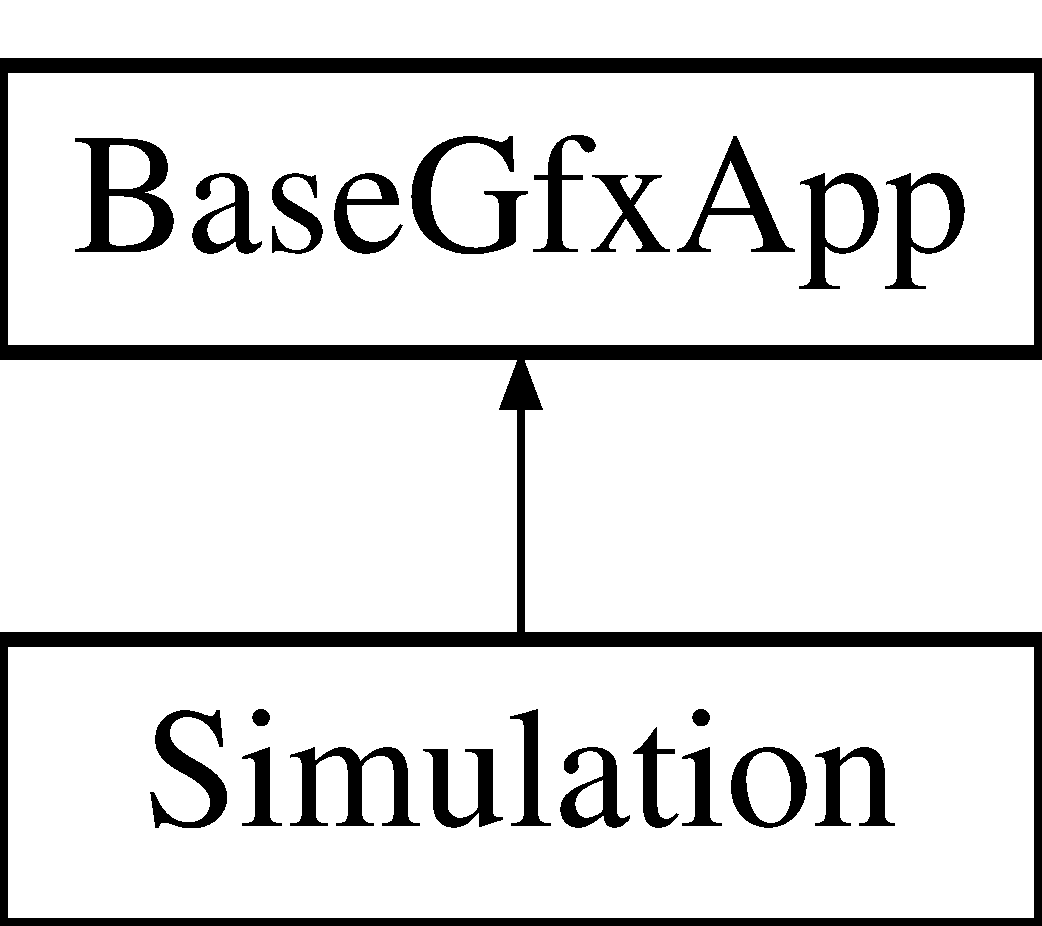
\includegraphics[height=2.000000cm]{classBaseGfxApp}
\end{center}
\end{figure}
\subsection*{Public Member Functions}
\begin{DoxyCompactItemize}
\item 
\hyperlink{classBaseGfxApp_a534a4b5293a35947fdae3805a103541d}{Base\-Gfx\-App} (int argc, char $\ast$argv\mbox{[}$\,$\mbox{]}, int \hyperlink{classBaseGfxApp_ace089a1a94fb6bb0bc17e1b7fa48e05d}{width}, int \hyperlink{classBaseGfxApp_aa253dbe16a20c40e0a1bf8ff942ceea3}{height}, int x, int y, int glut\-Flags, bool create\-G\-L\-U\-I\-Win, int glui\-Win\-X, int glui\-Win\-Y)
\item 
virtual \hyperlink{classBaseGfxApp_aceb6194bd818c0ffa980a6990fd03027}{$\sim$\-Base\-Gfx\-App} ()
\item 
void \hyperlink{classBaseGfxApp_a4b3b1a475b7f2babaf1b477c34b15fb1}{set\-Caption} (const std\-::string \&caption)
\item 
void \hyperlink{classBaseGfxApp_acda031916c00d56c2dc901e2653e3083}{run\-Main\-Loop} ()
\item 
virtual void \hyperlink{classBaseGfxApp_ac8de2d5a955582547af5619b771b4d6d}{display} ()
\item 
virtual void \hyperlink{classBaseGfxApp_a432317fc7c028b2c6702eb2232e85425}{advance} ()
\item 
virtual void \hyperlink{classBaseGfxApp_a0956b82d7fa58b623c498aea7073dbba}{mouse\-Moved} (int x, int y)
\item 
virtual void \hyperlink{classBaseGfxApp_abb23f716dd6612b3a72938e41525d338}{mouse\-Dragged} (int x, int y)
\item 
virtual void \hyperlink{classBaseGfxApp_aaaccf5a5e923a9465441a5ee712424a8}{left\-Mouse\-Down} (int x, int y)
\item 
virtual void \hyperlink{classBaseGfxApp_a0a2961a932b02b2f9d7d0bb408f6fb51}{left\-Mouse\-Up} (int x, int y)
\item 
virtual void \hyperlink{classBaseGfxApp_afa87e6a71220945e41f0424e540125d9}{right\-Mouse\-Down} (int x, int y)
\item 
virtual void \hyperlink{classBaseGfxApp_a812643d563522a993457dd565c33f8f6}{right\-Mouse\-Up} (int x, int y)
\item 
virtual void \hyperlink{classBaseGfxApp_a2c98cae9bb5ad1fb1832a6d4812670f8}{middle\-Mouse\-Down} (int x, int y)
\item 
virtual void \hyperlink{classBaseGfxApp_a00fc05e8d9629b72302b5adf014bdb0c}{middle\-Mouse\-Up} (int x, int y)
\item 
virtual void \hyperlink{classBaseGfxApp_a6d91e0cb7a3d48cad33956efe7eb36ca}{keyboard} (unsigned char c, int x, int y)
\item 
virtual void \hyperlink{classBaseGfxApp_a345566e62c9e4ec3705ec4d1c4c75f1f}{keyboard\-Special} (int key, int x, int y)
\item 
virtual void \hyperlink{classBaseGfxApp_acc4a40ce11edd6b6660a19cb4802a2bf}{keyboard\-Up} (unsigned char c, int x, int y)
\item 
virtual void \hyperlink{classBaseGfxApp_afd14b435ff93b1e7f461cb8bd1a6fd59}{keyboard\-Special\-Up} (int key, int x, int y)
\item 
virtual void \hyperlink{classBaseGfxApp_a5d8d5d778a8aecd7f5f8e9c87f4c3d20}{reshape} (int \hyperlink{classBaseGfxApp_ace089a1a94fb6bb0bc17e1b7fa48e05d}{width}, int \hyperlink{classBaseGfxApp_aa253dbe16a20c40e0a1bf8ff942ceea3}{height})
\item 
virtual void \hyperlink{classBaseGfxApp_a2978a7c358794c67df73b66776b2cef3}{glui\-Control} (int control\-I\-D)
\item 
int \hyperlink{classBaseGfxApp_ace089a1a94fb6bb0bc17e1b7fa48e05d}{width} () const 
\item 
int \hyperlink{classBaseGfxApp_aa253dbe16a20c40e0a1bf8ff942ceea3}{height} () const 
\item 
int \hyperlink{classBaseGfxApp_ae9779f948eff6f45beec08091e98a803}{handle} ()
\item 
G\-L\-U\-I $\ast$ \hyperlink{classBaseGfxApp_ac721a0fedce80308c5c0e5695016e95d}{glui} ()
\end{DoxyCompactItemize}
\subsection*{Static Public Member Functions}
\begin{DoxyCompactItemize}
\item 
static void \hyperlink{classBaseGfxApp_a4faec5e773876411a8b1912b0c1a0080}{graphics\-Begin} (int v, int delay)
\end{DoxyCompactItemize}
\subsection*{Static Protected Member Functions}
\begin{DoxyCompactItemize}
\item 
static void \hyperlink{classBaseGfxApp_a73c82d9170ffded2289883a8e47628a1}{graphics\-Timer} (int v)
\item 
static void \hyperlink{classBaseGfxApp_a5fe6a77d37044cbe28647ed3391bbb7a}{s\-\_\-reshape} (int \hyperlink{classBaseGfxApp_ace089a1a94fb6bb0bc17e1b7fa48e05d}{width}, int \hyperlink{classBaseGfxApp_aa253dbe16a20c40e0a1bf8ff942ceea3}{height})
\item 
static void \hyperlink{classBaseGfxApp_a52edb2569227319feb68779844e7d857}{s\-\_\-keyboard} (unsigned char c, int x, int y)
\item 
static void \hyperlink{classBaseGfxApp_a1e8d90a4faab60300ddf2a4ea9b83115}{s\-\_\-keyboardspecial} (int key, int x, int y)
\item 
static void \hyperlink{classBaseGfxApp_aa1ca205af9d6cee33949f2e6adf4c923}{s\-\_\-keyboardup} (unsigned char c, int x, int y)
\item 
static void \hyperlink{classBaseGfxApp_a0e4dfe006f3cc9126c1cc8ad32784f75}{s\-\_\-keyboardspecialup} (int key, int x, int y)
\item 
static void \hyperlink{classBaseGfxApp_a5e640f2394f7e038d0dd2b469d5c2e24}{s\-\_\-mousemotion} (int x, int y)
\item 
static void \hyperlink{classBaseGfxApp_a22dd953bfb75add9fd0f8f2f8be535c5}{s\-\_\-mousebtn} (int b, int s, int x, int y)
\item 
static void \hyperlink{classBaseGfxApp_a58415c6151a2a80e1fe2eaa9919a4dab}{s\-\_\-draw} ()
\item 
static void \hyperlink{classBaseGfxApp_ad4a963321f1147d68369225ab0c7f32f}{s\-\_\-gluicallback} (int control\-I\-D)
\end{DoxyCompactItemize}
\subsection*{Protected Attributes}
\begin{DoxyCompactItemize}
\item 
int \hyperlink{classBaseGfxApp_ad8697d6fdd10e6f336c3a662016b4fa7}{m\-\_\-glut\-Window\-Handle}
\item 
G\-L\-U\-I $\ast$ \hyperlink{classBaseGfxApp_a6eb1673b80283727221da2242211af1d}{m\-\_\-glui}
\item 
bool \hyperlink{classBaseGfxApp_a2e70a389224f8affe7c137f7e20dc8c1}{m\-\_\-drag}
\item 
int \hyperlink{classBaseGfxApp_a7e5ef1c8f25fe081b4a1fd4ce6a96e07}{m\-\_\-width}
\item 
int \hyperlink{classBaseGfxApp_ac078e4fc20b5c2fe0c744966b850b412}{m\-\_\-height}
\end{DoxyCompactItemize}
\subsection*{Static Protected Attributes}
\begin{DoxyCompactItemize}
\item 
static \hyperlink{classBaseGfxApp}{Base\-Gfx\-App} $\ast$ \hyperlink{classBaseGfxApp_a65ba89b98af31e2649a0546631931000}{s\-\_\-current\-App} = N\-U\-L\-L
\item 
static bool \hyperlink{classBaseGfxApp_afa4690383ea27713016ef75b9fb1e42f}{s\-\_\-glut\-Initialized} = false
\end{DoxyCompactItemize}


\subsection{Detailed Description}
Graphics driver class. 

\subsection{Constructor \& Destructor Documentation}
\hypertarget{classBaseGfxApp_a534a4b5293a35947fdae3805a103541d}{\index{Base\-Gfx\-App@{Base\-Gfx\-App}!Base\-Gfx\-App@{Base\-Gfx\-App}}
\index{Base\-Gfx\-App@{Base\-Gfx\-App}!BaseGfxApp@{Base\-Gfx\-App}}
\subsubsection[{Base\-Gfx\-App}]{\setlength{\rightskip}{0pt plus 5cm}Base\-Gfx\-App\-::\-Base\-Gfx\-App (
\begin{DoxyParamCaption}
\item[{int}]{argc, }
\item[{char $\ast$}]{argv\mbox{[}$\,$\mbox{]}, }
\item[{int}]{width, }
\item[{int}]{height, }
\item[{int}]{x, }
\item[{int}]{y, }
\item[{int}]{glut\-Flags, }
\item[{bool}]{create\-G\-L\-U\-I\-Win, }
\item[{int}]{glui\-Win\-X, }
\item[{int}]{glui\-Win\-Y}
\end{DoxyParamCaption}
)}}\label{classBaseGfxApp_a534a4b5293a35947fdae3805a103541d}
\hypertarget{classBaseGfxApp_aceb6194bd818c0ffa980a6990fd03027}{\index{Base\-Gfx\-App@{Base\-Gfx\-App}!$\sim$\-Base\-Gfx\-App@{$\sim$\-Base\-Gfx\-App}}
\index{$\sim$\-Base\-Gfx\-App@{$\sim$\-Base\-Gfx\-App}!BaseGfxApp@{Base\-Gfx\-App}}
\subsubsection[{$\sim$\-Base\-Gfx\-App}]{\setlength{\rightskip}{0pt plus 5cm}Base\-Gfx\-App\-::$\sim$\-Base\-Gfx\-App (
\begin{DoxyParamCaption}
{}
\end{DoxyParamCaption}
)\hspace{0.3cm}{\ttfamily [virtual]}}}\label{classBaseGfxApp_aceb6194bd818c0ffa980a6990fd03027}


\subsection{Member Function Documentation}
\hypertarget{classBaseGfxApp_a432317fc7c028b2c6702eb2232e85425}{\index{Base\-Gfx\-App@{Base\-Gfx\-App}!advance@{advance}}
\index{advance@{advance}!BaseGfxApp@{Base\-Gfx\-App}}
\subsubsection[{advance}]{\setlength{\rightskip}{0pt plus 5cm}virtual void Base\-Gfx\-App\-::advance (
\begin{DoxyParamCaption}
{}
\end{DoxyParamCaption}
)\hspace{0.3cm}{\ttfamily [inline]}, {\ttfamily [virtual]}}}\label{classBaseGfxApp_a432317fc7c028b2c6702eb2232e85425}


Reimplemented in \hyperlink{classSimulation_a4938ccecec0e9356cf547ef7bd5bbdf8}{Simulation}.

\hypertarget{classBaseGfxApp_ac8de2d5a955582547af5619b771b4d6d}{\index{Base\-Gfx\-App@{Base\-Gfx\-App}!display@{display}}
\index{display@{display}!BaseGfxApp@{Base\-Gfx\-App}}
\subsubsection[{display}]{\setlength{\rightskip}{0pt plus 5cm}virtual void Base\-Gfx\-App\-::display (
\begin{DoxyParamCaption}
{}
\end{DoxyParamCaption}
)\hspace{0.3cm}{\ttfamily [inline]}, {\ttfamily [virtual]}}}\label{classBaseGfxApp_ac8de2d5a955582547af5619b771b4d6d}


Reimplemented in \hyperlink{classSimulation_a449dcb7d97dfba99efe770de2f399c31}{Simulation}.

\hypertarget{classBaseGfxApp_ac721a0fedce80308c5c0e5695016e95d}{\index{Base\-Gfx\-App@{Base\-Gfx\-App}!glui@{glui}}
\index{glui@{glui}!BaseGfxApp@{Base\-Gfx\-App}}
\subsubsection[{glui}]{\setlength{\rightskip}{0pt plus 5cm}G\-L\-U\-I$\ast$ Base\-Gfx\-App\-::glui (
\begin{DoxyParamCaption}
{}
\end{DoxyParamCaption}
)\hspace{0.3cm}{\ttfamily [inline]}}}\label{classBaseGfxApp_ac721a0fedce80308c5c0e5695016e95d}
\hypertarget{classBaseGfxApp_a2978a7c358794c67df73b66776b2cef3}{\index{Base\-Gfx\-App@{Base\-Gfx\-App}!glui\-Control@{glui\-Control}}
\index{glui\-Control@{glui\-Control}!BaseGfxApp@{Base\-Gfx\-App}}
\subsubsection[{glui\-Control}]{\setlength{\rightskip}{0pt plus 5cm}virtual void Base\-Gfx\-App\-::glui\-Control (
\begin{DoxyParamCaption}
\item[{int}]{control\-I\-D}
\end{DoxyParamCaption}
)\hspace{0.3cm}{\ttfamily [inline]}, {\ttfamily [virtual]}}}\label{classBaseGfxApp_a2978a7c358794c67df73b66776b2cef3}


Reimplemented in \hyperlink{classSimulation_a1607cd18e552ab9f4a6f57d362f7121a}{Simulation}.

\hypertarget{classBaseGfxApp_a4faec5e773876411a8b1912b0c1a0080}{\index{Base\-Gfx\-App@{Base\-Gfx\-App}!graphics\-Begin@{graphics\-Begin}}
\index{graphics\-Begin@{graphics\-Begin}!BaseGfxApp@{Base\-Gfx\-App}}
\subsubsection[{graphics\-Begin}]{\setlength{\rightskip}{0pt plus 5cm}void Base\-Gfx\-App\-::graphics\-Begin (
\begin{DoxyParamCaption}
\item[{int}]{v, }
\item[{int}]{delay}
\end{DoxyParamCaption}
)\hspace{0.3cm}{\ttfamily [static]}}}\label{classBaseGfxApp_a4faec5e773876411a8b1912b0c1a0080}
This function starts the graphics after a delay. \hypertarget{classBaseGfxApp_a73c82d9170ffded2289883a8e47628a1}{\index{Base\-Gfx\-App@{Base\-Gfx\-App}!graphics\-Timer@{graphics\-Timer}}
\index{graphics\-Timer@{graphics\-Timer}!BaseGfxApp@{Base\-Gfx\-App}}
\subsubsection[{graphics\-Timer}]{\setlength{\rightskip}{0pt plus 5cm}void Base\-Gfx\-App\-::graphics\-Timer (
\begin{DoxyParamCaption}
\item[{int}]{v}
\end{DoxyParamCaption}
)\hspace{0.3cm}{\ttfamily [static]}, {\ttfamily [protected]}}}\label{classBaseGfxApp_a73c82d9170ffded2289883a8e47628a1}
This function calls itself using glut\-Timer\-Func once per frame. \hypertarget{classBaseGfxApp_ae9779f948eff6f45beec08091e98a803}{\index{Base\-Gfx\-App@{Base\-Gfx\-App}!handle@{handle}}
\index{handle@{handle}!BaseGfxApp@{Base\-Gfx\-App}}
\subsubsection[{handle}]{\setlength{\rightskip}{0pt plus 5cm}int Base\-Gfx\-App\-::handle (
\begin{DoxyParamCaption}
{}
\end{DoxyParamCaption}
)\hspace{0.3cm}{\ttfamily [inline]}}}\label{classBaseGfxApp_ae9779f948eff6f45beec08091e98a803}
\hypertarget{classBaseGfxApp_aa253dbe16a20c40e0a1bf8ff942ceea3}{\index{Base\-Gfx\-App@{Base\-Gfx\-App}!height@{height}}
\index{height@{height}!BaseGfxApp@{Base\-Gfx\-App}}
\subsubsection[{height}]{\setlength{\rightskip}{0pt plus 5cm}int Base\-Gfx\-App\-::height (
\begin{DoxyParamCaption}
{}
\end{DoxyParamCaption}
) const}}\label{classBaseGfxApp_aa253dbe16a20c40e0a1bf8ff942ceea3}
\hypertarget{classBaseGfxApp_a6d91e0cb7a3d48cad33956efe7eb36ca}{\index{Base\-Gfx\-App@{Base\-Gfx\-App}!keyboard@{keyboard}}
\index{keyboard@{keyboard}!BaseGfxApp@{Base\-Gfx\-App}}
\subsubsection[{keyboard}]{\setlength{\rightskip}{0pt plus 5cm}virtual void Base\-Gfx\-App\-::keyboard (
\begin{DoxyParamCaption}
\item[{unsigned char}]{c, }
\item[{int}]{x, }
\item[{int}]{y}
\end{DoxyParamCaption}
)\hspace{0.3cm}{\ttfamily [inline]}, {\ttfamily [virtual]}}}\label{classBaseGfxApp_a6d91e0cb7a3d48cad33956efe7eb36ca}


Reimplemented in \hyperlink{classSimulation_af2fc2b7caf1b85fb68c82375c3391569}{Simulation}.

\hypertarget{classBaseGfxApp_a345566e62c9e4ec3705ec4d1c4c75f1f}{\index{Base\-Gfx\-App@{Base\-Gfx\-App}!keyboard\-Special@{keyboard\-Special}}
\index{keyboard\-Special@{keyboard\-Special}!BaseGfxApp@{Base\-Gfx\-App}}
\subsubsection[{keyboard\-Special}]{\setlength{\rightskip}{0pt plus 5cm}virtual void Base\-Gfx\-App\-::keyboard\-Special (
\begin{DoxyParamCaption}
\item[{int}]{key, }
\item[{int}]{x, }
\item[{int}]{y}
\end{DoxyParamCaption}
)\hspace{0.3cm}{\ttfamily [inline]}, {\ttfamily [virtual]}}}\label{classBaseGfxApp_a345566e62c9e4ec3705ec4d1c4c75f1f}


Reimplemented in \hyperlink{classSimulation_ac60b25961b18057239efcb610b5c679f}{Simulation}.

\hypertarget{classBaseGfxApp_afd14b435ff93b1e7f461cb8bd1a6fd59}{\index{Base\-Gfx\-App@{Base\-Gfx\-App}!keyboard\-Special\-Up@{keyboard\-Special\-Up}}
\index{keyboard\-Special\-Up@{keyboard\-Special\-Up}!BaseGfxApp@{Base\-Gfx\-App}}
\subsubsection[{keyboard\-Special\-Up}]{\setlength{\rightskip}{0pt plus 5cm}virtual void Base\-Gfx\-App\-::keyboard\-Special\-Up (
\begin{DoxyParamCaption}
\item[{int}]{key, }
\item[{int}]{x, }
\item[{int}]{y}
\end{DoxyParamCaption}
)\hspace{0.3cm}{\ttfamily [inline]}, {\ttfamily [virtual]}}}\label{classBaseGfxApp_afd14b435ff93b1e7f461cb8bd1a6fd59}
\hypertarget{classBaseGfxApp_acc4a40ce11edd6b6660a19cb4802a2bf}{\index{Base\-Gfx\-App@{Base\-Gfx\-App}!keyboard\-Up@{keyboard\-Up}}
\index{keyboard\-Up@{keyboard\-Up}!BaseGfxApp@{Base\-Gfx\-App}}
\subsubsection[{keyboard\-Up}]{\setlength{\rightskip}{0pt plus 5cm}virtual void Base\-Gfx\-App\-::keyboard\-Up (
\begin{DoxyParamCaption}
\item[{unsigned char}]{c, }
\item[{int}]{x, }
\item[{int}]{y}
\end{DoxyParamCaption}
)\hspace{0.3cm}{\ttfamily [inline]}, {\ttfamily [virtual]}}}\label{classBaseGfxApp_acc4a40ce11edd6b6660a19cb4802a2bf}
\hypertarget{classBaseGfxApp_aaaccf5a5e923a9465441a5ee712424a8}{\index{Base\-Gfx\-App@{Base\-Gfx\-App}!left\-Mouse\-Down@{left\-Mouse\-Down}}
\index{left\-Mouse\-Down@{left\-Mouse\-Down}!BaseGfxApp@{Base\-Gfx\-App}}
\subsubsection[{left\-Mouse\-Down}]{\setlength{\rightskip}{0pt plus 5cm}virtual void Base\-Gfx\-App\-::left\-Mouse\-Down (
\begin{DoxyParamCaption}
\item[{int}]{x, }
\item[{int}]{y}
\end{DoxyParamCaption}
)\hspace{0.3cm}{\ttfamily [inline]}, {\ttfamily [virtual]}}}\label{classBaseGfxApp_aaaccf5a5e923a9465441a5ee712424a8}


Reimplemented in \hyperlink{classSimulation_a786d1ba31d29937f0ac6f3ea88f8a607}{Simulation}.

\hypertarget{classBaseGfxApp_a0a2961a932b02b2f9d7d0bb408f6fb51}{\index{Base\-Gfx\-App@{Base\-Gfx\-App}!left\-Mouse\-Up@{left\-Mouse\-Up}}
\index{left\-Mouse\-Up@{left\-Mouse\-Up}!BaseGfxApp@{Base\-Gfx\-App}}
\subsubsection[{left\-Mouse\-Up}]{\setlength{\rightskip}{0pt plus 5cm}virtual void Base\-Gfx\-App\-::left\-Mouse\-Up (
\begin{DoxyParamCaption}
\item[{int}]{x, }
\item[{int}]{y}
\end{DoxyParamCaption}
)\hspace{0.3cm}{\ttfamily [inline]}, {\ttfamily [virtual]}}}\label{classBaseGfxApp_a0a2961a932b02b2f9d7d0bb408f6fb51}


Reimplemented in \hyperlink{classSimulation_a62ef254d85017074cd521a5787b5a234}{Simulation}.

\hypertarget{classBaseGfxApp_a2c98cae9bb5ad1fb1832a6d4812670f8}{\index{Base\-Gfx\-App@{Base\-Gfx\-App}!middle\-Mouse\-Down@{middle\-Mouse\-Down}}
\index{middle\-Mouse\-Down@{middle\-Mouse\-Down}!BaseGfxApp@{Base\-Gfx\-App}}
\subsubsection[{middle\-Mouse\-Down}]{\setlength{\rightskip}{0pt plus 5cm}virtual void Base\-Gfx\-App\-::middle\-Mouse\-Down (
\begin{DoxyParamCaption}
\item[{int}]{x, }
\item[{int}]{y}
\end{DoxyParamCaption}
)\hspace{0.3cm}{\ttfamily [inline]}, {\ttfamily [virtual]}}}\label{classBaseGfxApp_a2c98cae9bb5ad1fb1832a6d4812670f8}


Reimplemented in \hyperlink{classSimulation_a4a8fb0f5c7cff8e747ae11d46653d18b}{Simulation}.

\hypertarget{classBaseGfxApp_a00fc05e8d9629b72302b5adf014bdb0c}{\index{Base\-Gfx\-App@{Base\-Gfx\-App}!middle\-Mouse\-Up@{middle\-Mouse\-Up}}
\index{middle\-Mouse\-Up@{middle\-Mouse\-Up}!BaseGfxApp@{Base\-Gfx\-App}}
\subsubsection[{middle\-Mouse\-Up}]{\setlength{\rightskip}{0pt plus 5cm}virtual void Base\-Gfx\-App\-::middle\-Mouse\-Up (
\begin{DoxyParamCaption}
\item[{int}]{x, }
\item[{int}]{y}
\end{DoxyParamCaption}
)\hspace{0.3cm}{\ttfamily [inline]}, {\ttfamily [virtual]}}}\label{classBaseGfxApp_a00fc05e8d9629b72302b5adf014bdb0c}
\hypertarget{classBaseGfxApp_abb23f716dd6612b3a72938e41525d338}{\index{Base\-Gfx\-App@{Base\-Gfx\-App}!mouse\-Dragged@{mouse\-Dragged}}
\index{mouse\-Dragged@{mouse\-Dragged}!BaseGfxApp@{Base\-Gfx\-App}}
\subsubsection[{mouse\-Dragged}]{\setlength{\rightskip}{0pt plus 5cm}virtual void Base\-Gfx\-App\-::mouse\-Dragged (
\begin{DoxyParamCaption}
\item[{int}]{x, }
\item[{int}]{y}
\end{DoxyParamCaption}
)\hspace{0.3cm}{\ttfamily [inline]}, {\ttfamily [virtual]}}}\label{classBaseGfxApp_abb23f716dd6612b3a72938e41525d338}


Reimplemented in \hyperlink{classSimulation_af942a4554aa7a45b468ea7e5bc2e0c4b}{Simulation}.

\hypertarget{classBaseGfxApp_a0956b82d7fa58b623c498aea7073dbba}{\index{Base\-Gfx\-App@{Base\-Gfx\-App}!mouse\-Moved@{mouse\-Moved}}
\index{mouse\-Moved@{mouse\-Moved}!BaseGfxApp@{Base\-Gfx\-App}}
\subsubsection[{mouse\-Moved}]{\setlength{\rightskip}{0pt plus 5cm}virtual void Base\-Gfx\-App\-::mouse\-Moved (
\begin{DoxyParamCaption}
\item[{int}]{x, }
\item[{int}]{y}
\end{DoxyParamCaption}
)\hspace{0.3cm}{\ttfamily [inline]}, {\ttfamily [virtual]}}}\label{classBaseGfxApp_a0956b82d7fa58b623c498aea7073dbba}
\hypertarget{classBaseGfxApp_a5d8d5d778a8aecd7f5f8e9c87f4c3d20}{\index{Base\-Gfx\-App@{Base\-Gfx\-App}!reshape@{reshape}}
\index{reshape@{reshape}!BaseGfxApp@{Base\-Gfx\-App}}
\subsubsection[{reshape}]{\setlength{\rightskip}{0pt plus 5cm}void Base\-Gfx\-App\-::reshape (
\begin{DoxyParamCaption}
\item[{int}]{width, }
\item[{int}]{height}
\end{DoxyParamCaption}
)\hspace{0.3cm}{\ttfamily [virtual]}}}\label{classBaseGfxApp_a5d8d5d778a8aecd7f5f8e9c87f4c3d20}
\hypertarget{classBaseGfxApp_afa87e6a71220945e41f0424e540125d9}{\index{Base\-Gfx\-App@{Base\-Gfx\-App}!right\-Mouse\-Down@{right\-Mouse\-Down}}
\index{right\-Mouse\-Down@{right\-Mouse\-Down}!BaseGfxApp@{Base\-Gfx\-App}}
\subsubsection[{right\-Mouse\-Down}]{\setlength{\rightskip}{0pt plus 5cm}virtual void Base\-Gfx\-App\-::right\-Mouse\-Down (
\begin{DoxyParamCaption}
\item[{int}]{x, }
\item[{int}]{y}
\end{DoxyParamCaption}
)\hspace{0.3cm}{\ttfamily [inline]}, {\ttfamily [virtual]}}}\label{classBaseGfxApp_afa87e6a71220945e41f0424e540125d9}
\hypertarget{classBaseGfxApp_a812643d563522a993457dd565c33f8f6}{\index{Base\-Gfx\-App@{Base\-Gfx\-App}!right\-Mouse\-Up@{right\-Mouse\-Up}}
\index{right\-Mouse\-Up@{right\-Mouse\-Up}!BaseGfxApp@{Base\-Gfx\-App}}
\subsubsection[{right\-Mouse\-Up}]{\setlength{\rightskip}{0pt plus 5cm}virtual void Base\-Gfx\-App\-::right\-Mouse\-Up (
\begin{DoxyParamCaption}
\item[{int}]{x, }
\item[{int}]{y}
\end{DoxyParamCaption}
)\hspace{0.3cm}{\ttfamily [inline]}, {\ttfamily [virtual]}}}\label{classBaseGfxApp_a812643d563522a993457dd565c33f8f6}
\hypertarget{classBaseGfxApp_acda031916c00d56c2dc901e2653e3083}{\index{Base\-Gfx\-App@{Base\-Gfx\-App}!run\-Main\-Loop@{run\-Main\-Loop}}
\index{run\-Main\-Loop@{run\-Main\-Loop}!BaseGfxApp@{Base\-Gfx\-App}}
\subsubsection[{run\-Main\-Loop}]{\setlength{\rightskip}{0pt plus 5cm}void Base\-Gfx\-App\-::run\-Main\-Loop (
\begin{DoxyParamCaption}
{}
\end{DoxyParamCaption}
)}}\label{classBaseGfxApp_acda031916c00d56c2dc901e2653e3083}
\hypertarget{classBaseGfxApp_a58415c6151a2a80e1fe2eaa9919a4dab}{\index{Base\-Gfx\-App@{Base\-Gfx\-App}!s\-\_\-draw@{s\-\_\-draw}}
\index{s\-\_\-draw@{s\-\_\-draw}!BaseGfxApp@{Base\-Gfx\-App}}
\subsubsection[{s\-\_\-draw}]{\setlength{\rightskip}{0pt plus 5cm}void Base\-Gfx\-App\-::s\-\_\-draw (
\begin{DoxyParamCaption}
{}
\end{DoxyParamCaption}
)\hspace{0.3cm}{\ttfamily [static]}, {\ttfamily [protected]}}}\label{classBaseGfxApp_a58415c6151a2a80e1fe2eaa9919a4dab}
\hypertarget{classBaseGfxApp_ad4a963321f1147d68369225ab0c7f32f}{\index{Base\-Gfx\-App@{Base\-Gfx\-App}!s\-\_\-gluicallback@{s\-\_\-gluicallback}}
\index{s\-\_\-gluicallback@{s\-\_\-gluicallback}!BaseGfxApp@{Base\-Gfx\-App}}
\subsubsection[{s\-\_\-gluicallback}]{\setlength{\rightskip}{0pt plus 5cm}void Base\-Gfx\-App\-::s\-\_\-gluicallback (
\begin{DoxyParamCaption}
\item[{int}]{control\-I\-D}
\end{DoxyParamCaption}
)\hspace{0.3cm}{\ttfamily [static]}, {\ttfamily [protected]}}}\label{classBaseGfxApp_ad4a963321f1147d68369225ab0c7f32f}
\hypertarget{classBaseGfxApp_a52edb2569227319feb68779844e7d857}{\index{Base\-Gfx\-App@{Base\-Gfx\-App}!s\-\_\-keyboard@{s\-\_\-keyboard}}
\index{s\-\_\-keyboard@{s\-\_\-keyboard}!BaseGfxApp@{Base\-Gfx\-App}}
\subsubsection[{s\-\_\-keyboard}]{\setlength{\rightskip}{0pt plus 5cm}void Base\-Gfx\-App\-::s\-\_\-keyboard (
\begin{DoxyParamCaption}
\item[{unsigned char}]{c, }
\item[{int}]{x, }
\item[{int}]{y}
\end{DoxyParamCaption}
)\hspace{0.3cm}{\ttfamily [static]}, {\ttfamily [protected]}}}\label{classBaseGfxApp_a52edb2569227319feb68779844e7d857}
\hypertarget{classBaseGfxApp_a1e8d90a4faab60300ddf2a4ea9b83115}{\index{Base\-Gfx\-App@{Base\-Gfx\-App}!s\-\_\-keyboardspecial@{s\-\_\-keyboardspecial}}
\index{s\-\_\-keyboardspecial@{s\-\_\-keyboardspecial}!BaseGfxApp@{Base\-Gfx\-App}}
\subsubsection[{s\-\_\-keyboardspecial}]{\setlength{\rightskip}{0pt plus 5cm}void Base\-Gfx\-App\-::s\-\_\-keyboardspecial (
\begin{DoxyParamCaption}
\item[{int}]{key, }
\item[{int}]{x, }
\item[{int}]{y}
\end{DoxyParamCaption}
)\hspace{0.3cm}{\ttfamily [static]}, {\ttfamily [protected]}}}\label{classBaseGfxApp_a1e8d90a4faab60300ddf2a4ea9b83115}
\hypertarget{classBaseGfxApp_a0e4dfe006f3cc9126c1cc8ad32784f75}{\index{Base\-Gfx\-App@{Base\-Gfx\-App}!s\-\_\-keyboardspecialup@{s\-\_\-keyboardspecialup}}
\index{s\-\_\-keyboardspecialup@{s\-\_\-keyboardspecialup}!BaseGfxApp@{Base\-Gfx\-App}}
\subsubsection[{s\-\_\-keyboardspecialup}]{\setlength{\rightskip}{0pt plus 5cm}void Base\-Gfx\-App\-::s\-\_\-keyboardspecialup (
\begin{DoxyParamCaption}
\item[{int}]{key, }
\item[{int}]{x, }
\item[{int}]{y}
\end{DoxyParamCaption}
)\hspace{0.3cm}{\ttfamily [static]}, {\ttfamily [protected]}}}\label{classBaseGfxApp_a0e4dfe006f3cc9126c1cc8ad32784f75}
\hypertarget{classBaseGfxApp_aa1ca205af9d6cee33949f2e6adf4c923}{\index{Base\-Gfx\-App@{Base\-Gfx\-App}!s\-\_\-keyboardup@{s\-\_\-keyboardup}}
\index{s\-\_\-keyboardup@{s\-\_\-keyboardup}!BaseGfxApp@{Base\-Gfx\-App}}
\subsubsection[{s\-\_\-keyboardup}]{\setlength{\rightskip}{0pt plus 5cm}void Base\-Gfx\-App\-::s\-\_\-keyboardup (
\begin{DoxyParamCaption}
\item[{unsigned char}]{c, }
\item[{int}]{x, }
\item[{int}]{y}
\end{DoxyParamCaption}
)\hspace{0.3cm}{\ttfamily [static]}, {\ttfamily [protected]}}}\label{classBaseGfxApp_aa1ca205af9d6cee33949f2e6adf4c923}
\hypertarget{classBaseGfxApp_a22dd953bfb75add9fd0f8f2f8be535c5}{\index{Base\-Gfx\-App@{Base\-Gfx\-App}!s\-\_\-mousebtn@{s\-\_\-mousebtn}}
\index{s\-\_\-mousebtn@{s\-\_\-mousebtn}!BaseGfxApp@{Base\-Gfx\-App}}
\subsubsection[{s\-\_\-mousebtn}]{\setlength{\rightskip}{0pt plus 5cm}void Base\-Gfx\-App\-::s\-\_\-mousebtn (
\begin{DoxyParamCaption}
\item[{int}]{b, }
\item[{int}]{s, }
\item[{int}]{x, }
\item[{int}]{y}
\end{DoxyParamCaption}
)\hspace{0.3cm}{\ttfamily [static]}, {\ttfamily [protected]}}}\label{classBaseGfxApp_a22dd953bfb75add9fd0f8f2f8be535c5}
\hypertarget{classBaseGfxApp_a5e640f2394f7e038d0dd2b469d5c2e24}{\index{Base\-Gfx\-App@{Base\-Gfx\-App}!s\-\_\-mousemotion@{s\-\_\-mousemotion}}
\index{s\-\_\-mousemotion@{s\-\_\-mousemotion}!BaseGfxApp@{Base\-Gfx\-App}}
\subsubsection[{s\-\_\-mousemotion}]{\setlength{\rightskip}{0pt plus 5cm}void Base\-Gfx\-App\-::s\-\_\-mousemotion (
\begin{DoxyParamCaption}
\item[{int}]{x, }
\item[{int}]{y}
\end{DoxyParamCaption}
)\hspace{0.3cm}{\ttfamily [static]}, {\ttfamily [protected]}}}\label{classBaseGfxApp_a5e640f2394f7e038d0dd2b469d5c2e24}
\hypertarget{classBaseGfxApp_a5fe6a77d37044cbe28647ed3391bbb7a}{\index{Base\-Gfx\-App@{Base\-Gfx\-App}!s\-\_\-reshape@{s\-\_\-reshape}}
\index{s\-\_\-reshape@{s\-\_\-reshape}!BaseGfxApp@{Base\-Gfx\-App}}
\subsubsection[{s\-\_\-reshape}]{\setlength{\rightskip}{0pt plus 5cm}void Base\-Gfx\-App\-::s\-\_\-reshape (
\begin{DoxyParamCaption}
\item[{int}]{width, }
\item[{int}]{height}
\end{DoxyParamCaption}
)\hspace{0.3cm}{\ttfamily [static]}, {\ttfamily [protected]}}}\label{classBaseGfxApp_a5fe6a77d37044cbe28647ed3391bbb7a}
\hypertarget{classBaseGfxApp_a4b3b1a475b7f2babaf1b477c34b15fb1}{\index{Base\-Gfx\-App@{Base\-Gfx\-App}!set\-Caption@{set\-Caption}}
\index{set\-Caption@{set\-Caption}!BaseGfxApp@{Base\-Gfx\-App}}
\subsubsection[{set\-Caption}]{\setlength{\rightskip}{0pt plus 5cm}void Base\-Gfx\-App\-::set\-Caption (
\begin{DoxyParamCaption}
\item[{const std\-::string \&}]{caption}
\end{DoxyParamCaption}
)}}\label{classBaseGfxApp_a4b3b1a475b7f2babaf1b477c34b15fb1}
\hypertarget{classBaseGfxApp_ace089a1a94fb6bb0bc17e1b7fa48e05d}{\index{Base\-Gfx\-App@{Base\-Gfx\-App}!width@{width}}
\index{width@{width}!BaseGfxApp@{Base\-Gfx\-App}}
\subsubsection[{width}]{\setlength{\rightskip}{0pt plus 5cm}int Base\-Gfx\-App\-::width (
\begin{DoxyParamCaption}
{}
\end{DoxyParamCaption}
) const}}\label{classBaseGfxApp_ace089a1a94fb6bb0bc17e1b7fa48e05d}


\subsection{Member Data Documentation}
\hypertarget{classBaseGfxApp_a2e70a389224f8affe7c137f7e20dc8c1}{\index{Base\-Gfx\-App@{Base\-Gfx\-App}!m\-\_\-drag@{m\-\_\-drag}}
\index{m\-\_\-drag@{m\-\_\-drag}!BaseGfxApp@{Base\-Gfx\-App}}
\subsubsection[{m\-\_\-drag}]{\setlength{\rightskip}{0pt plus 5cm}bool Base\-Gfx\-App\-::m\-\_\-drag\hspace{0.3cm}{\ttfamily [protected]}}}\label{classBaseGfxApp_a2e70a389224f8affe7c137f7e20dc8c1}
\hypertarget{classBaseGfxApp_a6eb1673b80283727221da2242211af1d}{\index{Base\-Gfx\-App@{Base\-Gfx\-App}!m\-\_\-glui@{m\-\_\-glui}}
\index{m\-\_\-glui@{m\-\_\-glui}!BaseGfxApp@{Base\-Gfx\-App}}
\subsubsection[{m\-\_\-glui}]{\setlength{\rightskip}{0pt plus 5cm}G\-L\-U\-I$\ast$ Base\-Gfx\-App\-::m\-\_\-glui\hspace{0.3cm}{\ttfamily [protected]}}}\label{classBaseGfxApp_a6eb1673b80283727221da2242211af1d}
\hypertarget{classBaseGfxApp_ad8697d6fdd10e6f336c3a662016b4fa7}{\index{Base\-Gfx\-App@{Base\-Gfx\-App}!m\-\_\-glut\-Window\-Handle@{m\-\_\-glut\-Window\-Handle}}
\index{m\-\_\-glut\-Window\-Handle@{m\-\_\-glut\-Window\-Handle}!BaseGfxApp@{Base\-Gfx\-App}}
\subsubsection[{m\-\_\-glut\-Window\-Handle}]{\setlength{\rightskip}{0pt plus 5cm}int Base\-Gfx\-App\-::m\-\_\-glut\-Window\-Handle\hspace{0.3cm}{\ttfamily [protected]}}}\label{classBaseGfxApp_ad8697d6fdd10e6f336c3a662016b4fa7}
Underlying glut window handle \hypertarget{classBaseGfxApp_ac078e4fc20b5c2fe0c744966b850b412}{\index{Base\-Gfx\-App@{Base\-Gfx\-App}!m\-\_\-height@{m\-\_\-height}}
\index{m\-\_\-height@{m\-\_\-height}!BaseGfxApp@{Base\-Gfx\-App}}
\subsubsection[{m\-\_\-height}]{\setlength{\rightskip}{0pt plus 5cm}int Base\-Gfx\-App\-::m\-\_\-height\hspace{0.3cm}{\ttfamily [protected]}}}\label{classBaseGfxApp_ac078e4fc20b5c2fe0c744966b850b412}
\hypertarget{classBaseGfxApp_a7e5ef1c8f25fe081b4a1fd4ce6a96e07}{\index{Base\-Gfx\-App@{Base\-Gfx\-App}!m\-\_\-width@{m\-\_\-width}}
\index{m\-\_\-width@{m\-\_\-width}!BaseGfxApp@{Base\-Gfx\-App}}
\subsubsection[{m\-\_\-width}]{\setlength{\rightskip}{0pt plus 5cm}int Base\-Gfx\-App\-::m\-\_\-width\hspace{0.3cm}{\ttfamily [protected]}}}\label{classBaseGfxApp_a7e5ef1c8f25fe081b4a1fd4ce6a96e07}
\hypertarget{classBaseGfxApp_a65ba89b98af31e2649a0546631931000}{\index{Base\-Gfx\-App@{Base\-Gfx\-App}!s\-\_\-current\-App@{s\-\_\-current\-App}}
\index{s\-\_\-current\-App@{s\-\_\-current\-App}!BaseGfxApp@{Base\-Gfx\-App}}
\subsubsection[{s\-\_\-current\-App}]{\setlength{\rightskip}{0pt plus 5cm}{\bf Base\-Gfx\-App} $\ast$ Base\-Gfx\-App\-::s\-\_\-current\-App = N\-U\-L\-L\hspace{0.3cm}{\ttfamily [static]}, {\ttfamily [protected]}}}\label{classBaseGfxApp_a65ba89b98af31e2649a0546631931000}
G\-L\-U\-T and G\-L\-U\-I event callbacks are sent to the current window/app. Right now, there is only one window anyway (not counting the G\-L\-U\-I U\-I window.. in the future could be extended to support more windows. In any case, some structure like this is always needed when using glut with C++, since the glut callbacks must be either global or static functions. \hypertarget{classBaseGfxApp_afa4690383ea27713016ef75b9fb1e42f}{\index{Base\-Gfx\-App@{Base\-Gfx\-App}!s\-\_\-glut\-Initialized@{s\-\_\-glut\-Initialized}}
\index{s\-\_\-glut\-Initialized@{s\-\_\-glut\-Initialized}!BaseGfxApp@{Base\-Gfx\-App}}
\subsubsection[{s\-\_\-glut\-Initialized}]{\setlength{\rightskip}{0pt plus 5cm}bool Base\-Gfx\-App\-::s\-\_\-glut\-Initialized = false\hspace{0.3cm}{\ttfamily [static]}, {\ttfamily [protected]}}}\label{classBaseGfxApp_afa4690383ea27713016ef75b9fb1e42f}
Has glut\-Init been called? (only allowed once per program) 

The documentation for this class was generated from the following files\-:\begin{DoxyCompactItemize}
\item 
\hyperlink{BaseGfxApp_8h}{Base\-Gfx\-App.\-h}\item 
\hyperlink{BaseGfxApp_8cpp}{Base\-Gfx\-App.\-cpp}\end{DoxyCompactItemize}

\hypertarget{structColor}{\section{Color Struct Reference}
\label{structColor}\index{Color@{Color}}
}


This struct holds the representation of a color.  




{\ttfamily \#include $<$Color.\-h$>$}

\subsection*{Public Member Functions}
\begin{DoxyCompactItemize}
\item 
\hyperlink{structColor_a9a742cbe9f9f4037f5d9f4e81a9b2428}{Color} ()
\item 
\hyperlink{structColor_a373c542c99fb83ce9c7c08aae76b2718}{Color} (float r, float g, float b)
\item 
\hyperlink{structColor_ade5cd4cc07dfaf745089dce14e47c31b}{Color} (char c)
\begin{DoxyCompactList}\small\item\em Creates a R\-G\-B color from its char color name  The following is the list of allowed colors\-: \end{DoxyCompactList}\item 
\hyperlink{structColor_a2023dcb2762807f60730e0787abc4788}{Color} (int c)
\begin{DoxyCompactList}\small\item\em Creates an R\-G\-B color from a hex value  The color is stored as the last 3 bytes, as 0x$<$unused (set to 0)$>$$<$red$>$$<$green$>$$<$blue$>$\par
 Each byte is interpreted as an integer holding an R\-G\-B value from 0-\/255. These are then converted to floats between 0 and 1 by dividing by 255. Note that this requires at least 3 byte integers. \end{DoxyCompactList}\item 
bool \hyperlink{structColor_a93e73674565d6205f8c777aeb2a05524}{is\-Similar} (\hyperlink{structColor}{Color} c1)
\begin{DoxyCompactList}\small\item\em Checks if two colors are similar. \end{DoxyCompactList}\item 
std\-::ostream \& \hyperlink{structColor_a0af0a6b6bc80cdb89f39a931c003ebc7}{operator$<$$<$} (std\-::ostream \&out)
\item 
bool \hyperlink{structColor_a4d6e2671c47f5e65a98f1a2fd0792d4e}{operator==} (\hyperlink{structColor}{Color} c1)
\begin{DoxyCompactList}\small\item\em Checks if two colors are equal. \end{DoxyCompactList}\item 
bool \hyperlink{structColor_ad4d11eb4823a1dbb9d37c7b5fbe708a4}{operator!=} (\hyperlink{structColor}{Color} c1)
\begin{DoxyCompactList}\small\item\em Checks if two colors are not equal. \end{DoxyCompactList}\end{DoxyCompactItemize}
\subsection*{Public Attributes}
\begin{DoxyCompactItemize}
\item 
float \hyperlink{structColor_aa897fe858468c4bff0f286d0dfd43178}{red}
\item 
float \hyperlink{structColor_a7644dc2e2c23e40894929ce5127452a1}{green}
\item 
float \hyperlink{structColor_a175386a89265cede8f6ae694c32677c3}{blue}
\end{DoxyCompactItemize}


\subsection{Detailed Description}
This struct holds the representation of a color. 

Each field is a float value that shoult be between 0 and 1. This allows a direct translation from hex colors, with each field being the hex R\-G\-B value / 255. 

\subsection{Constructor \& Destructor Documentation}
\hypertarget{structColor_a9a742cbe9f9f4037f5d9f4e81a9b2428}{\index{Color@{Color}!Color@{Color}}
\index{Color@{Color}!Color@{Color}}
\subsubsection[{Color}]{\setlength{\rightskip}{0pt plus 5cm}Color\-::\-Color (
\begin{DoxyParamCaption}
{}
\end{DoxyParamCaption}
)\hspace{0.3cm}{\ttfamily [inline]}}}\label{structColor_a9a742cbe9f9f4037f5d9f4e81a9b2428}
\hypertarget{structColor_a373c542c99fb83ce9c7c08aae76b2718}{\index{Color@{Color}!Color@{Color}}
\index{Color@{Color}!Color@{Color}}
\subsubsection[{Color}]{\setlength{\rightskip}{0pt plus 5cm}Color\-::\-Color (
\begin{DoxyParamCaption}
\item[{float}]{r, }
\item[{float}]{g, }
\item[{float}]{b}
\end{DoxyParamCaption}
)\hspace{0.3cm}{\ttfamily [inline]}}}\label{structColor_a373c542c99fb83ce9c7c08aae76b2718}
\hypertarget{structColor_ade5cd4cc07dfaf745089dce14e47c31b}{\index{Color@{Color}!Color@{Color}}
\index{Color@{Color}!Color@{Color}}
\subsubsection[{Color}]{\setlength{\rightskip}{0pt plus 5cm}Color\-::\-Color (
\begin{DoxyParamCaption}
\item[{char}]{c}
\end{DoxyParamCaption}
)}}\label{structColor_ade5cd4cc07dfaf745089dce14e47c31b}


Creates a R\-G\-B color from its char color name  The following is the list of allowed colors\-: 

\begin{DoxyAuthor}{Author}
Lucas Kramer \begin{TabularC}{3}
\hline
{\bfseries \hyperlink{structColor}{Color} char} &{\bfseries \hyperlink{structColor}{Color} name} &{\bfseries R\-G\-B floating-\/point value}  \\\cline{1-3}
'R' &Red &(1, 0, 0)  \\\cline{1-3}
'O' &Orange &(1, 0.\-4, 0)  \\\cline{1-3}
'Y' &Yellow &(1, 1, 0)  \\\cline{1-3}
'G' &Green &(0, 1, 0)  \\\cline{1-3}
'B' &Blue &(0, 0, 1)  \\\cline{1-3}
'V' &Violet &(0.\-5, 0, 0.\-5)  \\\cline{1-3}
'W' &White &(1, 1, 1)  \\\cline{1-3}
default &Black &(0, 0, 0)  \\\cline{1-3}
\end{TabularC}

\end{DoxyAuthor}
\hypertarget{structColor_a2023dcb2762807f60730e0787abc4788}{\index{Color@{Color}!Color@{Color}}
\index{Color@{Color}!Color@{Color}}
\subsubsection[{Color}]{\setlength{\rightskip}{0pt plus 5cm}Color\-::\-Color (
\begin{DoxyParamCaption}
\item[{int}]{c}
\end{DoxyParamCaption}
)}}\label{structColor_a2023dcb2762807f60730e0787abc4788}


Creates an R\-G\-B color from a hex value  The color is stored as the last 3 bytes, as 0x$<$unused (set to 0)$>$$<$red$>$$<$green$>$$<$blue$>$\par
 Each byte is interpreted as an integer holding an R\-G\-B value from 0-\/255. These are then converted to floats between 0 and 1 by dividing by 255. Note that this requires at least 3 byte integers. 

\begin{DoxyAuthor}{Author}
Carl Bahn  Lucas Kramer 
\end{DoxyAuthor}


\subsection{Member Function Documentation}
\hypertarget{structColor_a93e73674565d6205f8c777aeb2a05524}{\index{Color@{Color}!is\-Similar@{is\-Similar}}
\index{is\-Similar@{is\-Similar}!Color@{Color}}
\subsubsection[{is\-Similar}]{\setlength{\rightskip}{0pt plus 5cm}bool Color\-::is\-Similar (
\begin{DoxyParamCaption}
\item[{{\bf Color}}]{c1}
\end{DoxyParamCaption}
)}}\label{structColor_a93e73674565d6205f8c777aeb2a05524}


Checks if two colors are similar. 

\begin{DoxyAuthor}{Author}
Lucas Kramer 
\end{DoxyAuthor}

\begin{DoxyParams}{Parameters}
{\em c1} & the color to compare \\
\hline
\end{DoxyParams}
\begin{DoxyReturn}{Returns}
true if the colors are similar 
\end{DoxyReturn}
\hypertarget{structColor_ad4d11eb4823a1dbb9d37c7b5fbe708a4}{\index{Color@{Color}!operator!=@{operator!=}}
\index{operator!=@{operator!=}!Color@{Color}}
\subsubsection[{operator!=}]{\setlength{\rightskip}{0pt plus 5cm}bool Color\-::operator!= (
\begin{DoxyParamCaption}
\item[{{\bf Color}}]{c1}
\end{DoxyParamCaption}
)}}\label{structColor_ad4d11eb4823a1dbb9d37c7b5fbe708a4}


Checks if two colors are not equal. 

\begin{DoxyAuthor}{Author}
Lucas Kramer 
\end{DoxyAuthor}

\begin{DoxyParams}{Parameters}
{\em c1} & the color to check \\
\hline
\end{DoxyParams}
\begin{DoxyReturn}{Returns}
true if the colors are not equal 
\end{DoxyReturn}
\hypertarget{structColor_a0af0a6b6bc80cdb89f39a931c003ebc7}{\index{Color@{Color}!operator$<$$<$@{operator$<$$<$}}
\index{operator$<$$<$@{operator$<$$<$}!Color@{Color}}
\subsubsection[{operator$<$$<$}]{\setlength{\rightskip}{0pt plus 5cm}std\-::ostream\& Color\-::operator$<$$<$ (
\begin{DoxyParamCaption}
\item[{std\-::ostream \&}]{out}
\end{DoxyParamCaption}
)\hspace{0.3cm}{\ttfamily [inline]}}}\label{structColor_a0af0a6b6bc80cdb89f39a931c003ebc7}
\hypertarget{structColor_a4d6e2671c47f5e65a98f1a2fd0792d4e}{\index{Color@{Color}!operator==@{operator==}}
\index{operator==@{operator==}!Color@{Color}}
\subsubsection[{operator==}]{\setlength{\rightskip}{0pt plus 5cm}bool Color\-::operator== (
\begin{DoxyParamCaption}
\item[{{\bf Color}}]{c1}
\end{DoxyParamCaption}
)}}\label{structColor_a4d6e2671c47f5e65a98f1a2fd0792d4e}


Checks if two colors are equal. 

\begin{DoxyAuthor}{Author}
Lucas Kramer 
\end{DoxyAuthor}

\begin{DoxyParams}{Parameters}
{\em c1} & the color to check \\
\hline
\end{DoxyParams}
\begin{DoxyReturn}{Returns}
true if the colors are equal 
\end{DoxyReturn}


\subsection{Member Data Documentation}
\hypertarget{structColor_a175386a89265cede8f6ae694c32677c3}{\index{Color@{Color}!blue@{blue}}
\index{blue@{blue}!Color@{Color}}
\subsubsection[{blue}]{\setlength{\rightskip}{0pt plus 5cm}float Color\-::blue}}\label{structColor_a175386a89265cede8f6ae694c32677c3}
\hypertarget{structColor_a7644dc2e2c23e40894929ce5127452a1}{\index{Color@{Color}!green@{green}}
\index{green@{green}!Color@{Color}}
\subsubsection[{green}]{\setlength{\rightskip}{0pt plus 5cm}float Color\-::green}}\label{structColor_a7644dc2e2c23e40894929ce5127452a1}
\hypertarget{structColor_aa897fe858468c4bff0f286d0dfd43178}{\index{Color@{Color}!red@{red}}
\index{red@{red}!Color@{Color}}
\subsubsection[{red}]{\setlength{\rightskip}{0pt plus 5cm}float Color\-::red}}\label{structColor_aa897fe858468c4bff0f286d0dfd43178}


The documentation for this struct was generated from the following files\-:\begin{DoxyCompactItemize}
\item 
\hyperlink{Color_8h}{Color.\-h}\item 
\hyperlink{Color_8cpp}{Color.\-cpp}\end{DoxyCompactItemize}

\hypertarget{classComplexRobot}{\section{Complex\-Robot Class Reference}
\label{classComplexRobot}\index{Complex\-Robot@{Complex\-Robot}}
}


A complex robot with configurable feedback from all sensors.  




{\ttfamily \#include $<$Complex\-Robot.\-h$>$}

Inheritance diagram for Complex\-Robot\-:\begin{figure}[H]
\begin{center}
\leavevmode
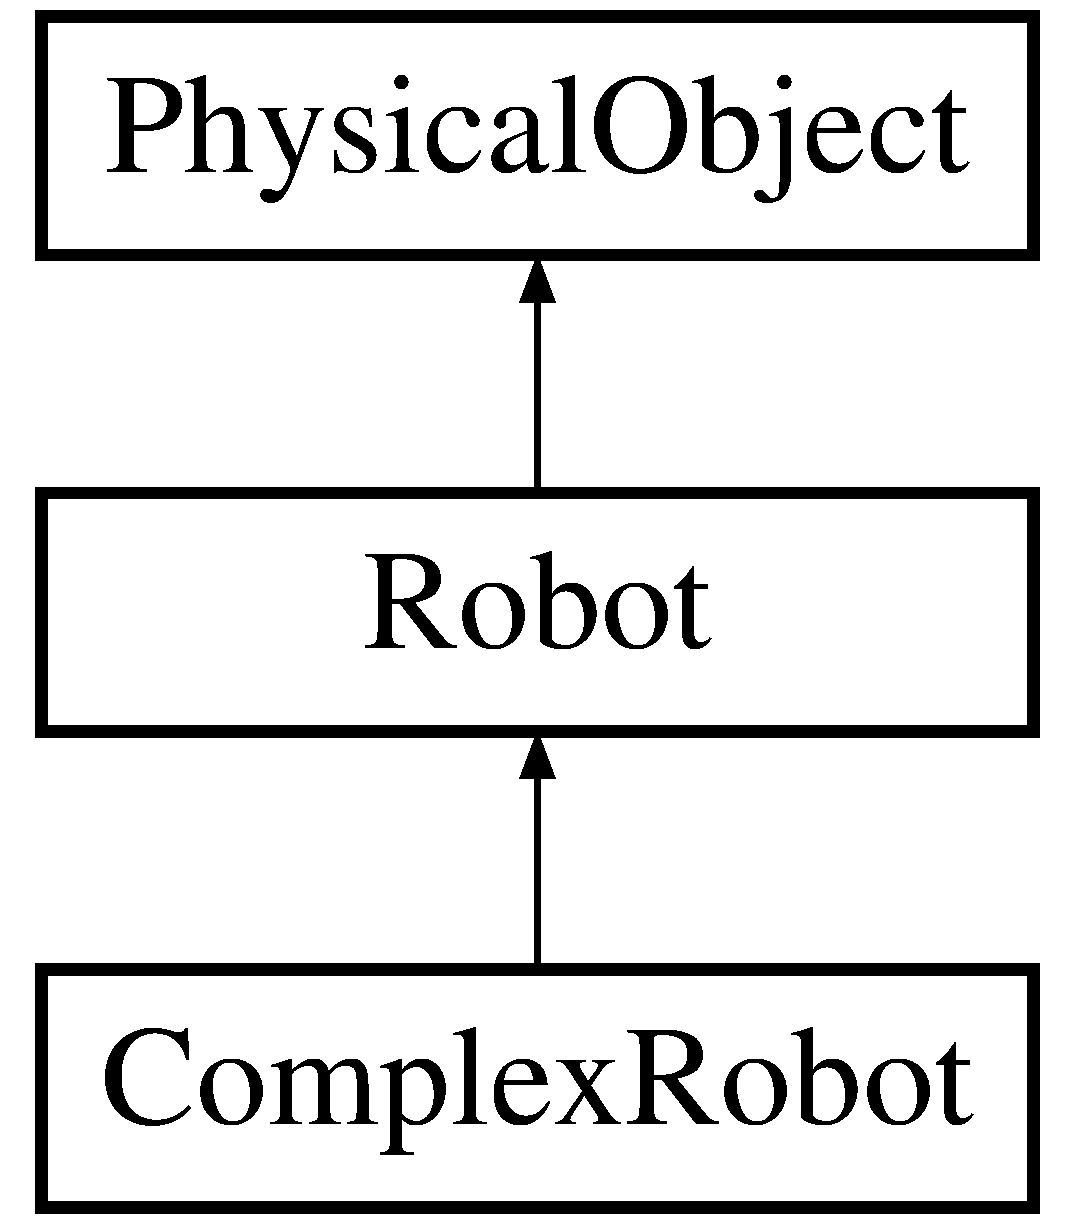
\includegraphics[height=3.000000cm]{classComplexRobot}
\end{center}
\end{figure}
\subsection*{Public Member Functions}
\begin{DoxyCompactItemize}
\item 
\hyperlink{classComplexRobot_ac1c27bb32c2bc66f7b34317947b3fc17}{Complex\-Robot} ()
\item 
\hyperlink{classComplexRobot_a3e45d7e3a708c5c44908bb360a04e656}{Complex\-Robot} (int radius, \hyperlink{structColor}{Color} color, \hyperlink{structColor}{Color} line\-Color, bool \hyperlink{classComplexRobot_a371e0363adebfa9898b7db2827e62216}{enable\-Light\-Sensors}, bool \hyperlink{classComplexRobot_afbd7060c1ba7505825bd8a6d87755c57}{enable\-Robot\-Sensors}, bool \hyperlink{classComplexRobot_a1a92f81d958c5497dad6c0fb470193e6}{enable\-Obstacle\-Sensors}, bool \hyperlink{classComplexRobot_a5480d20648fefda9eab9e3a31cb74a8e}{enable\-Target\-Sensors}, bool \hyperlink{classComplexRobot_a56421342335d639c79fce6c4087e92ba}{light\-Sensors\-Crossed}, bool \hyperlink{classComplexRobot_a329fa033f98c4611fc6fd08f1ec0c1a2}{robot\-Sensors\-Crossed}, bool \hyperlink{classComplexRobot_aa1bbfff6b94d790366c903e8ee9d7c35}{obstacle\-Sensors\-Crossed}, bool \hyperlink{classComplexRobot_ac7fa0582f9c586b38c1dc73382a1c5a9}{target\-Sensors\-Crossed}, float \hyperlink{classComplexRobot_afb1bda51a4a0d99fa2eea1fe8f7ee240}{light\-Sensor\-Scale}, float \hyperlink{classComplexRobot_ac433b802cfc866917bc32680357e0b3e}{robot\-Sensor\-Scale}, float \hyperlink{classComplexRobot_a62e4d0dafe87412f5d868a3a7a462209}{obstacle\-Sensor\-Scale}, float \hyperlink{classComplexRobot_a95cae4898e63c23418684c87e6ab0176}{target\-Sensor\-Scale}, int \hyperlink{classComplexRobot_a38ae464727dfb577e24a2b4c1a305e5d}{default\-Speed}, int target\-Id=-\/1)
\item 
\hyperlink{classComplexRobot_a45c21b79ada7a4cce275e4c94c62c01f}{Complex\-Robot} (int radius, \hyperlink{structLocation}{Location} loc, \hyperlink{structColor}{Color} color, \hyperlink{structColor}{Color} line\-Color, bool \hyperlink{classComplexRobot_a371e0363adebfa9898b7db2827e62216}{enable\-Light\-Sensors}, bool \hyperlink{classComplexRobot_afbd7060c1ba7505825bd8a6d87755c57}{enable\-Robot\-Sensors}, bool \hyperlink{classComplexRobot_a1a92f81d958c5497dad6c0fb470193e6}{enable\-Obstacle\-Sensors}, bool \hyperlink{classComplexRobot_a5480d20648fefda9eab9e3a31cb74a8e}{enable\-Target\-Sensors}, bool \hyperlink{classComplexRobot_a56421342335d639c79fce6c4087e92ba}{light\-Sensors\-Crossed}, bool \hyperlink{classComplexRobot_a329fa033f98c4611fc6fd08f1ec0c1a2}{robot\-Sensors\-Crossed}, bool \hyperlink{classComplexRobot_aa1bbfff6b94d790366c903e8ee9d7c35}{obstacle\-Sensors\-Crossed}, bool \hyperlink{classComplexRobot_ac7fa0582f9c586b38c1dc73382a1c5a9}{target\-Sensors\-Crossed}, float \hyperlink{classComplexRobot_afb1bda51a4a0d99fa2eea1fe8f7ee240}{light\-Sensor\-Scale}, float \hyperlink{classComplexRobot_ac433b802cfc866917bc32680357e0b3e}{robot\-Sensor\-Scale}, float \hyperlink{classComplexRobot_a62e4d0dafe87412f5d868a3a7a462209}{obstacle\-Sensor\-Scale}, float \hyperlink{classComplexRobot_a95cae4898e63c23418684c87e6ab0176}{target\-Sensor\-Scale}, int \hyperlink{classComplexRobot_a38ae464727dfb577e24a2b4c1a305e5d}{default\-Speed}, int target\-Id=-\/1)
\item 
\hyperlink{classComplexRobot_a4ce778d818e7ad00d2ef47a387f12865}{$\sim$\-Complex\-Robot} ()
\item 
float \hyperlink{classComplexRobot_aa50c7f5ed4f288987fe2557b41a9bf32}{get\-Left\-Speed} (float left\-Light\-Sensor\-Val, float right\-Light\-Sensor\-Val, float left\-Robot\-Sensor\-Val, float right\-Robot\-Sensor\-Val, float left\-Obstacle\-Sensor\-Val, float right\-Obstacle\-Sensor\-Val, float left\-Target\-Sensor\-Val, float right\-Target\-Sensor\-Val)
\item 
float \hyperlink{classComplexRobot_ac038c2dbcc242d68a3ef9e533673bdf6}{get\-Right\-Speed} (float left\-Light\-Sensor\-Val, float right\-Light\-Sensor\-Val, float left\-Robot\-Sensor\-Val, float right\-Robot\-Sensor\-Val, float left\-Obstacle\-Sensor\-Val, float right\-Obstacle\-Sensor\-Val, float left\-Target\-Sensor\-Val, float right\-Target\-Sensor\-Val)
\end{DoxyCompactItemize}
\subsection*{Public Attributes}
\begin{DoxyCompactItemize}
\item 
const bool \hyperlink{classComplexRobot_a371e0363adebfa9898b7db2827e62216}{enable\-Light\-Sensors}
\item 
const bool \hyperlink{classComplexRobot_afbd7060c1ba7505825bd8a6d87755c57}{enable\-Robot\-Sensors}
\item 
const bool \hyperlink{classComplexRobot_a1a92f81d958c5497dad6c0fb470193e6}{enable\-Obstacle\-Sensors}
\item 
const bool \hyperlink{classComplexRobot_a5480d20648fefda9eab9e3a31cb74a8e}{enable\-Target\-Sensors}
\item 
const bool \hyperlink{classComplexRobot_a56421342335d639c79fce6c4087e92ba}{light\-Sensors\-Crossed}
\item 
const bool \hyperlink{classComplexRobot_a329fa033f98c4611fc6fd08f1ec0c1a2}{robot\-Sensors\-Crossed}
\item 
const bool \hyperlink{classComplexRobot_aa1bbfff6b94d790366c903e8ee9d7c35}{obstacle\-Sensors\-Crossed}
\item 
const bool \hyperlink{classComplexRobot_ac7fa0582f9c586b38c1dc73382a1c5a9}{target\-Sensors\-Crossed}
\item 
const float \hyperlink{classComplexRobot_afb1bda51a4a0d99fa2eea1fe8f7ee240}{light\-Sensor\-Scale}
\item 
const float \hyperlink{classComplexRobot_ac433b802cfc866917bc32680357e0b3e}{robot\-Sensor\-Scale}
\item 
const float \hyperlink{classComplexRobot_a62e4d0dafe87412f5d868a3a7a462209}{obstacle\-Sensor\-Scale}
\item 
const float \hyperlink{classComplexRobot_a95cae4898e63c23418684c87e6ab0176}{target\-Sensor\-Scale}
\item 
const int \hyperlink{classComplexRobot_a38ae464727dfb577e24a2b4c1a305e5d}{default\-Speed}
\end{DoxyCompactItemize}
\subsection*{Additional Inherited Members}


\subsection{Detailed Description}
A complex robot with configurable feedback from all sensors. 

\subsection{Constructor \& Destructor Documentation}
\hypertarget{classComplexRobot_ac1c27bb32c2bc66f7b34317947b3fc17}{\index{Complex\-Robot@{Complex\-Robot}!Complex\-Robot@{Complex\-Robot}}
\index{Complex\-Robot@{Complex\-Robot}!ComplexRobot@{Complex\-Robot}}
\subsubsection[{Complex\-Robot}]{\setlength{\rightskip}{0pt plus 5cm}Complex\-Robot\-::\-Complex\-Robot (
\begin{DoxyParamCaption}
{}
\end{DoxyParamCaption}
)}}\label{classComplexRobot_ac1c27bb32c2bc66f7b34317947b3fc17}
\hypertarget{classComplexRobot_a3e45d7e3a708c5c44908bb360a04e656}{\index{Complex\-Robot@{Complex\-Robot}!Complex\-Robot@{Complex\-Robot}}
\index{Complex\-Robot@{Complex\-Robot}!ComplexRobot@{Complex\-Robot}}
\subsubsection[{Complex\-Robot}]{\setlength{\rightskip}{0pt plus 5cm}Complex\-Robot\-::\-Complex\-Robot (
\begin{DoxyParamCaption}
\item[{int}]{radius, }
\item[{{\bf Color}}]{color, }
\item[{{\bf Color}}]{line\-Color, }
\item[{bool}]{enable\-Light\-Sensors, }
\item[{bool}]{enable\-Robot\-Sensors, }
\item[{bool}]{enable\-Obstacle\-Sensors, }
\item[{bool}]{enable\-Target\-Sensors, }
\item[{bool}]{light\-Sensors\-Crossed, }
\item[{bool}]{robot\-Sensors\-Crossed, }
\item[{bool}]{obstacle\-Sensors\-Crossed, }
\item[{bool}]{target\-Sensors\-Crossed, }
\item[{float}]{light\-Sensor\-Scale, }
\item[{float}]{robot\-Sensor\-Scale, }
\item[{float}]{obstacle\-Sensor\-Scale, }
\item[{float}]{target\-Sensor\-Scale, }
\item[{int}]{default\-Speed, }
\item[{int}]{target\-Id = {\ttfamily -\/1}}
\end{DoxyParamCaption}
)}}\label{classComplexRobot_a3e45d7e3a708c5c44908bb360a04e656}
\hypertarget{classComplexRobot_a45c21b79ada7a4cce275e4c94c62c01f}{\index{Complex\-Robot@{Complex\-Robot}!Complex\-Robot@{Complex\-Robot}}
\index{Complex\-Robot@{Complex\-Robot}!ComplexRobot@{Complex\-Robot}}
\subsubsection[{Complex\-Robot}]{\setlength{\rightskip}{0pt plus 5cm}Complex\-Robot\-::\-Complex\-Robot (
\begin{DoxyParamCaption}
\item[{int}]{radius, }
\item[{{\bf Location}}]{loc, }
\item[{{\bf Color}}]{color, }
\item[{{\bf Color}}]{line\-Color, }
\item[{bool}]{enable\-Light\-Sensors, }
\item[{bool}]{enable\-Robot\-Sensors, }
\item[{bool}]{enable\-Obstacle\-Sensors, }
\item[{bool}]{enable\-Target\-Sensors, }
\item[{bool}]{light\-Sensors\-Crossed, }
\item[{bool}]{robot\-Sensors\-Crossed, }
\item[{bool}]{obstacle\-Sensors\-Crossed, }
\item[{bool}]{target\-Sensors\-Crossed, }
\item[{float}]{light\-Sensor\-Scale, }
\item[{float}]{robot\-Sensor\-Scale, }
\item[{float}]{obstacle\-Sensor\-Scale, }
\item[{float}]{target\-Sensor\-Scale, }
\item[{int}]{default\-Speed, }
\item[{int}]{target\-Id = {\ttfamily -\/1}}
\end{DoxyParamCaption}
)}}\label{classComplexRobot_a45c21b79ada7a4cce275e4c94c62c01f}
\hypertarget{classComplexRobot_a4ce778d818e7ad00d2ef47a387f12865}{\index{Complex\-Robot@{Complex\-Robot}!$\sim$\-Complex\-Robot@{$\sim$\-Complex\-Robot}}
\index{$\sim$\-Complex\-Robot@{$\sim$\-Complex\-Robot}!ComplexRobot@{Complex\-Robot}}
\subsubsection[{$\sim$\-Complex\-Robot}]{\setlength{\rightskip}{0pt plus 5cm}Complex\-Robot\-::$\sim$\-Complex\-Robot (
\begin{DoxyParamCaption}
{}
\end{DoxyParamCaption}
)}}\label{classComplexRobot_a4ce778d818e7ad00d2ef47a387f12865}


\subsection{Member Function Documentation}
\hypertarget{classComplexRobot_aa50c7f5ed4f288987fe2557b41a9bf32}{\index{Complex\-Robot@{Complex\-Robot}!get\-Left\-Speed@{get\-Left\-Speed}}
\index{get\-Left\-Speed@{get\-Left\-Speed}!ComplexRobot@{Complex\-Robot}}
\subsubsection[{get\-Left\-Speed}]{\setlength{\rightskip}{0pt plus 5cm}float Complex\-Robot\-::get\-Left\-Speed (
\begin{DoxyParamCaption}
\item[{float}]{left\-Light\-Sensor\-Val, }
\item[{float}]{right\-Light\-Sensor\-Val, }
\item[{float}]{left\-Robot\-Sensor\-Val, }
\item[{float}]{right\-Robot\-Sensor\-Val, }
\item[{float}]{left\-Obstacle\-Sensor\-Val, }
\item[{float}]{right\-Obstacle\-Sensor\-Val, }
\item[{float}]{left\-Target\-Sensor\-Val, }
\item[{float}]{right\-Target\-Sensor\-Val}
\end{DoxyParamCaption}
)\hspace{0.3cm}{\ttfamily [virtual]}}}\label{classComplexRobot_aa50c7f5ed4f288987fe2557b41a9bf32}


Implements \hyperlink{classRobot_a9c96f301ae826e7c535f6b705e44bcd6}{Robot}.

\hypertarget{classComplexRobot_ac038c2dbcc242d68a3ef9e533673bdf6}{\index{Complex\-Robot@{Complex\-Robot}!get\-Right\-Speed@{get\-Right\-Speed}}
\index{get\-Right\-Speed@{get\-Right\-Speed}!ComplexRobot@{Complex\-Robot}}
\subsubsection[{get\-Right\-Speed}]{\setlength{\rightskip}{0pt plus 5cm}float Complex\-Robot\-::get\-Right\-Speed (
\begin{DoxyParamCaption}
\item[{float}]{left\-Light\-Sensor\-Val, }
\item[{float}]{right\-Light\-Sensor\-Val, }
\item[{float}]{left\-Robot\-Sensor\-Val, }
\item[{float}]{right\-Robot\-Sensor\-Val, }
\item[{float}]{left\-Obstacle\-Sensor\-Val, }
\item[{float}]{right\-Obstacle\-Sensor\-Val, }
\item[{float}]{left\-Target\-Sensor\-Val, }
\item[{float}]{right\-Target\-Sensor\-Val}
\end{DoxyParamCaption}
)\hspace{0.3cm}{\ttfamily [virtual]}}}\label{classComplexRobot_ac038c2dbcc242d68a3ef9e533673bdf6}


Implements \hyperlink{classRobot_a3289251979084c50b18a6006547d3f95}{Robot}.



\subsection{Member Data Documentation}
\hypertarget{classComplexRobot_a38ae464727dfb577e24a2b4c1a305e5d}{\index{Complex\-Robot@{Complex\-Robot}!default\-Speed@{default\-Speed}}
\index{default\-Speed@{default\-Speed}!ComplexRobot@{Complex\-Robot}}
\subsubsection[{default\-Speed}]{\setlength{\rightskip}{0pt plus 5cm}const int Complex\-Robot\-::default\-Speed}}\label{classComplexRobot_a38ae464727dfb577e24a2b4c1a305e5d}
\hypertarget{classComplexRobot_a371e0363adebfa9898b7db2827e62216}{\index{Complex\-Robot@{Complex\-Robot}!enable\-Light\-Sensors@{enable\-Light\-Sensors}}
\index{enable\-Light\-Sensors@{enable\-Light\-Sensors}!ComplexRobot@{Complex\-Robot}}
\subsubsection[{enable\-Light\-Sensors}]{\setlength{\rightskip}{0pt plus 5cm}const bool Complex\-Robot\-::enable\-Light\-Sensors}}\label{classComplexRobot_a371e0363adebfa9898b7db2827e62216}
\hypertarget{classComplexRobot_a1a92f81d958c5497dad6c0fb470193e6}{\index{Complex\-Robot@{Complex\-Robot}!enable\-Obstacle\-Sensors@{enable\-Obstacle\-Sensors}}
\index{enable\-Obstacle\-Sensors@{enable\-Obstacle\-Sensors}!ComplexRobot@{Complex\-Robot}}
\subsubsection[{enable\-Obstacle\-Sensors}]{\setlength{\rightskip}{0pt plus 5cm}const bool Complex\-Robot\-::enable\-Obstacle\-Sensors}}\label{classComplexRobot_a1a92f81d958c5497dad6c0fb470193e6}
\hypertarget{classComplexRobot_afbd7060c1ba7505825bd8a6d87755c57}{\index{Complex\-Robot@{Complex\-Robot}!enable\-Robot\-Sensors@{enable\-Robot\-Sensors}}
\index{enable\-Robot\-Sensors@{enable\-Robot\-Sensors}!ComplexRobot@{Complex\-Robot}}
\subsubsection[{enable\-Robot\-Sensors}]{\setlength{\rightskip}{0pt plus 5cm}const bool Complex\-Robot\-::enable\-Robot\-Sensors}}\label{classComplexRobot_afbd7060c1ba7505825bd8a6d87755c57}
\hypertarget{classComplexRobot_a5480d20648fefda9eab9e3a31cb74a8e}{\index{Complex\-Robot@{Complex\-Robot}!enable\-Target\-Sensors@{enable\-Target\-Sensors}}
\index{enable\-Target\-Sensors@{enable\-Target\-Sensors}!ComplexRobot@{Complex\-Robot}}
\subsubsection[{enable\-Target\-Sensors}]{\setlength{\rightskip}{0pt plus 5cm}const bool Complex\-Robot\-::enable\-Target\-Sensors}}\label{classComplexRobot_a5480d20648fefda9eab9e3a31cb74a8e}
\hypertarget{classComplexRobot_afb1bda51a4a0d99fa2eea1fe8f7ee240}{\index{Complex\-Robot@{Complex\-Robot}!light\-Sensor\-Scale@{light\-Sensor\-Scale}}
\index{light\-Sensor\-Scale@{light\-Sensor\-Scale}!ComplexRobot@{Complex\-Robot}}
\subsubsection[{light\-Sensor\-Scale}]{\setlength{\rightskip}{0pt plus 5cm}const float Complex\-Robot\-::light\-Sensor\-Scale}}\label{classComplexRobot_afb1bda51a4a0d99fa2eea1fe8f7ee240}
\hypertarget{classComplexRobot_a56421342335d639c79fce6c4087e92ba}{\index{Complex\-Robot@{Complex\-Robot}!light\-Sensors\-Crossed@{light\-Sensors\-Crossed}}
\index{light\-Sensors\-Crossed@{light\-Sensors\-Crossed}!ComplexRobot@{Complex\-Robot}}
\subsubsection[{light\-Sensors\-Crossed}]{\setlength{\rightskip}{0pt plus 5cm}const bool Complex\-Robot\-::light\-Sensors\-Crossed}}\label{classComplexRobot_a56421342335d639c79fce6c4087e92ba}
\hypertarget{classComplexRobot_a62e4d0dafe87412f5d868a3a7a462209}{\index{Complex\-Robot@{Complex\-Robot}!obstacle\-Sensor\-Scale@{obstacle\-Sensor\-Scale}}
\index{obstacle\-Sensor\-Scale@{obstacle\-Sensor\-Scale}!ComplexRobot@{Complex\-Robot}}
\subsubsection[{obstacle\-Sensor\-Scale}]{\setlength{\rightskip}{0pt plus 5cm}const float Complex\-Robot\-::obstacle\-Sensor\-Scale}}\label{classComplexRobot_a62e4d0dafe87412f5d868a3a7a462209}
\hypertarget{classComplexRobot_aa1bbfff6b94d790366c903e8ee9d7c35}{\index{Complex\-Robot@{Complex\-Robot}!obstacle\-Sensors\-Crossed@{obstacle\-Sensors\-Crossed}}
\index{obstacle\-Sensors\-Crossed@{obstacle\-Sensors\-Crossed}!ComplexRobot@{Complex\-Robot}}
\subsubsection[{obstacle\-Sensors\-Crossed}]{\setlength{\rightskip}{0pt plus 5cm}const bool Complex\-Robot\-::obstacle\-Sensors\-Crossed}}\label{classComplexRobot_aa1bbfff6b94d790366c903e8ee9d7c35}
\hypertarget{classComplexRobot_ac433b802cfc866917bc32680357e0b3e}{\index{Complex\-Robot@{Complex\-Robot}!robot\-Sensor\-Scale@{robot\-Sensor\-Scale}}
\index{robot\-Sensor\-Scale@{robot\-Sensor\-Scale}!ComplexRobot@{Complex\-Robot}}
\subsubsection[{robot\-Sensor\-Scale}]{\setlength{\rightskip}{0pt plus 5cm}const float Complex\-Robot\-::robot\-Sensor\-Scale}}\label{classComplexRobot_ac433b802cfc866917bc32680357e0b3e}
\hypertarget{classComplexRobot_a329fa033f98c4611fc6fd08f1ec0c1a2}{\index{Complex\-Robot@{Complex\-Robot}!robot\-Sensors\-Crossed@{robot\-Sensors\-Crossed}}
\index{robot\-Sensors\-Crossed@{robot\-Sensors\-Crossed}!ComplexRobot@{Complex\-Robot}}
\subsubsection[{robot\-Sensors\-Crossed}]{\setlength{\rightskip}{0pt plus 5cm}const bool Complex\-Robot\-::robot\-Sensors\-Crossed}}\label{classComplexRobot_a329fa033f98c4611fc6fd08f1ec0c1a2}
\hypertarget{classComplexRobot_a95cae4898e63c23418684c87e6ab0176}{\index{Complex\-Robot@{Complex\-Robot}!target\-Sensor\-Scale@{target\-Sensor\-Scale}}
\index{target\-Sensor\-Scale@{target\-Sensor\-Scale}!ComplexRobot@{Complex\-Robot}}
\subsubsection[{target\-Sensor\-Scale}]{\setlength{\rightskip}{0pt plus 5cm}const float Complex\-Robot\-::target\-Sensor\-Scale}}\label{classComplexRobot_a95cae4898e63c23418684c87e6ab0176}
\hypertarget{classComplexRobot_ac7fa0582f9c586b38c1dc73382a1c5a9}{\index{Complex\-Robot@{Complex\-Robot}!target\-Sensors\-Crossed@{target\-Sensors\-Crossed}}
\index{target\-Sensors\-Crossed@{target\-Sensors\-Crossed}!ComplexRobot@{Complex\-Robot}}
\subsubsection[{target\-Sensors\-Crossed}]{\setlength{\rightskip}{0pt plus 5cm}const bool Complex\-Robot\-::target\-Sensors\-Crossed}}\label{classComplexRobot_ac7fa0582f9c586b38c1dc73382a1c5a9}


The documentation for this class was generated from the following files\-:\begin{DoxyCompactItemize}
\item 
\hyperlink{ComplexRobot_8h}{Complex\-Robot.\-h}\item 
\hyperlink{ComplexRobot_8cpp}{Complex\-Robot.\-cpp}\end{DoxyCompactItemize}

\hypertarget{classLightSource}{\section{Light\-Source Class Reference}
\label{classLightSource}\index{Light\-Source@{Light\-Source}}
}


\hyperlink{classLightSource}{Light\-Source} for the robot to seek.  




{\ttfamily \#include $<$Light\-Source.\-h$>$}

Inheritance diagram for Light\-Source\-:\begin{figure}[H]
\begin{center}
\leavevmode
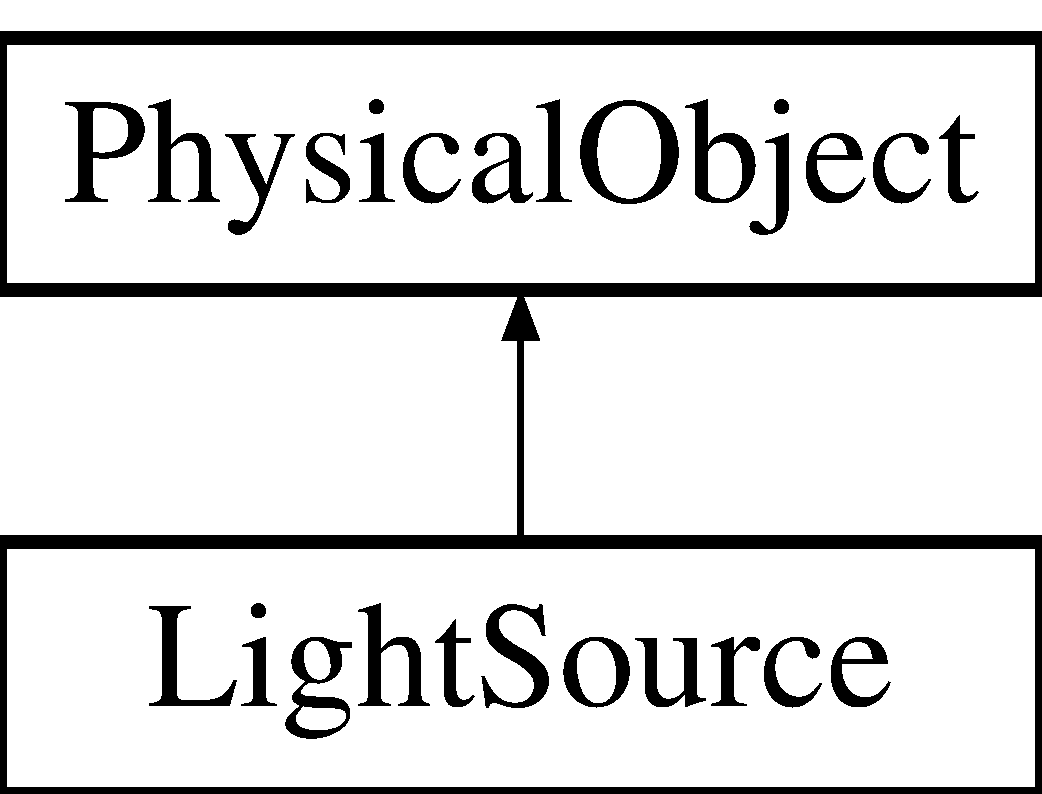
\includegraphics[height=2.000000cm]{classLightSource}
\end{center}
\end{figure}
\subsection*{Public Member Functions}
\begin{DoxyCompactItemize}
\item 
\hyperlink{classLightSource_a11168d72f5e489b8d4b5c6056682e5fa}{Light\-Source} (int radius, \hyperlink{structColor}{Color} color)
\item 
\hyperlink{classLightSource_aa13ee0c57818324958659a5a88bf4b1d}{Light\-Source} (int max\-Radius, int min\-Radius, \hyperlink{structColor}{Color} color)
\item 
\hyperlink{classLightSource_a953998d4d97c0efda733c208258e4a8b}{Light\-Source} (int radius, \hyperlink{structLocation}{Location} loc, \hyperlink{structColor}{Color} color)
\item 
bool \hyperlink{classLightSource_a6c0da63e11edd3f108c9fe8c2a9dfd52}{handle\-Collision} (int other\-Id, bool was\-Hit)
\item 
\hyperlink{classLightSource_a55e5876407fd4af9e9b4ede7ff46cc85}{$\sim$\-Light\-Source} ()
\item 
void \hyperlink{classLightSource_a2148117298a6bb0d60dcfb3bd99700db}{display} ()
\end{DoxyCompactItemize}
\subsection*{Additional Inherited Members}


\subsection{Detailed Description}
\hyperlink{classLightSource}{Light\-Source} for the robot to seek. 

\subsection{Constructor \& Destructor Documentation}
\hypertarget{classLightSource_a11168d72f5e489b8d4b5c6056682e5fa}{\index{Light\-Source@{Light\-Source}!Light\-Source@{Light\-Source}}
\index{Light\-Source@{Light\-Source}!LightSource@{Light\-Source}}
\subsubsection[{Light\-Source}]{\setlength{\rightskip}{0pt plus 5cm}Light\-Source\-::\-Light\-Source (
\begin{DoxyParamCaption}
\item[{int}]{radius, }
\item[{{\bf Color}}]{color}
\end{DoxyParamCaption}
)}}\label{classLightSource_a11168d72f5e489b8d4b5c6056682e5fa}
This constructor requires two parameters\-: radius and color) 
\begin{DoxyParams}{Parameters}
{\em radius} & the radius in pixels \\
\hline
{\em color} & a struct of float value 0 to 1 representing a hexedecimal color \\
\hline
\end{DoxyParams}
\begin{DoxyParagraph}{Initialization}
\hyperlink{classLightSource}{Light\-Source} is initialized with the following values\-: 
\end{DoxyParagraph}


Orientation\-: random 

Speed\-: 0 

Position\-: (loc.\-x, loc.\-y)   \hypertarget{classLightSource_aa13ee0c57818324958659a5a88bf4b1d}{\index{Light\-Source@{Light\-Source}!Light\-Source@{Light\-Source}}
\index{Light\-Source@{Light\-Source}!LightSource@{Light\-Source}}
\subsubsection[{Light\-Source}]{\setlength{\rightskip}{0pt plus 5cm}Light\-Source\-::\-Light\-Source (
\begin{DoxyParamCaption}
\item[{int}]{max\-Radius, }
\item[{int}]{min\-Radius, }
\item[{{\bf Color}}]{color}
\end{DoxyParamCaption}
)}}\label{classLightSource_aa13ee0c57818324958659a5a88bf4b1d}
This constructor creates a light with a random radius 
\begin{DoxyParams}{Parameters}
{\em min\-Radius} & the minimum possible radius in pixels \\
\hline
{\em max\-Radius} & the maximum possible radius in pixels \\
\hline
{\em color} & a struct representing color \\
\hline
\end{DoxyParams}
\begin{DoxyParagraph}{Initialization}
\hyperlink{classLightSource}{Light\-Source} is initialized with the following values\-: 
\end{DoxyParagraph}


Orientation\-: random 

Speed\-: 0 

Position\-: (loc.\-x, loc.\-y)   \hypertarget{classLightSource_a953998d4d97c0efda733c208258e4a8b}{\index{Light\-Source@{Light\-Source}!Light\-Source@{Light\-Source}}
\index{Light\-Source@{Light\-Source}!LightSource@{Light\-Source}}
\subsubsection[{Light\-Source}]{\setlength{\rightskip}{0pt plus 5cm}Light\-Source\-::\-Light\-Source (
\begin{DoxyParamCaption}
\item[{int}]{radius, }
\item[{{\bf Location}}]{loc, }
\item[{{\bf Color}}]{color}
\end{DoxyParamCaption}
)}}\label{classLightSource_a953998d4d97c0efda733c208258e4a8b}
This constructor requires four parameters\-: radius, color, start \hyperlink{structLocation}{Location} and Config\-Table value) 
\begin{DoxyParams}{Parameters}
{\em radius} & the radius in pixels \\
\hline
{\em color} & a struct of float value 0 to 1 representing a hexedecimal color \\
\hline
{\em loc} & a struct of the x,y start \hyperlink{structLocation}{Location} in pixels \\
\hline
{\em config} & a configuration table \\
\hline
\end{DoxyParams}
\begin{DoxyParagraph}{Initialization}
\hyperlink{classLightSource}{Light\-Source} is initialized with the following values\-: 
\end{DoxyParagraph}


Orientation\-: 0 

Speed\-: 0 

Position\-: (loc.\-x, loc.\-y)   \hypertarget{classLightSource_a55e5876407fd4af9e9b4ede7ff46cc85}{\index{Light\-Source@{Light\-Source}!$\sim$\-Light\-Source@{$\sim$\-Light\-Source}}
\index{$\sim$\-Light\-Source@{$\sim$\-Light\-Source}!LightSource@{Light\-Source}}
\subsubsection[{$\sim$\-Light\-Source}]{\setlength{\rightskip}{0pt plus 5cm}Light\-Source\-::$\sim$\-Light\-Source (
\begin{DoxyParamCaption}
{}
\end{DoxyParamCaption}
)}}\label{classLightSource_a55e5876407fd4af9e9b4ede7ff46cc85}
This is the class destructor. 

\subsection{Member Function Documentation}
\hypertarget{classLightSource_a2148117298a6bb0d60dcfb3bd99700db}{\index{Light\-Source@{Light\-Source}!display@{display}}
\index{display@{display}!LightSource@{Light\-Source}}
\subsubsection[{display}]{\setlength{\rightskip}{0pt plus 5cm}void Light\-Source\-::display (
\begin{DoxyParamCaption}
{}
\end{DoxyParamCaption}
)\hspace{0.3cm}{\ttfamily [virtual]}}}\label{classLightSource_a2148117298a6bb0d60dcfb3bd99700db}
This function displays the \hyperlink{classLightSource}{Light\-Source} in the graphics. 

Reimplemented from \hyperlink{classPhysicalObject_a6a0326df3efc0a1ea23892e3fcd4b11e}{Physical\-Object}.

\hypertarget{classLightSource_a6c0da63e11edd3f108c9fe8c2a9dfd52}{\index{Light\-Source@{Light\-Source}!handle\-Collision@{handle\-Collision}}
\index{handle\-Collision@{handle\-Collision}!LightSource@{Light\-Source}}
\subsubsection[{handle\-Collision}]{\setlength{\rightskip}{0pt plus 5cm}bool Light\-Source\-::handle\-Collision (
\begin{DoxyParamCaption}
\item[{int}]{other\-Id, }
\item[{bool}]{was\-Hit}
\end{DoxyParamCaption}
)\hspace{0.3cm}{\ttfamily [virtual]}}}\label{classLightSource_a6c0da63e11edd3f108c9fe8c2a9dfd52}
\begin{DoxyAuthor}{Author}
Lucas Kramer This function gives \hyperlink{classLightSource}{Light\-Source} an appropriate reaction when a collision occurs. 
\end{DoxyAuthor}

\begin{DoxyParams}{Parameters}
{\em other\-Id} & id of the object that it collides with \\
\hline
{\em was\-Hit} & tells if the object was hit previously \\
\hline
\end{DoxyParams}


Implements \hyperlink{classPhysicalObject_a400ba3545479ebbf8b1b4a046906e562}{Physical\-Object}.



The documentation for this class was generated from the following files\-:\begin{DoxyCompactItemize}
\item 
\hyperlink{LightSource_8h}{Light\-Source.\-h}\item 
\hyperlink{LightSource_8cpp}{Light\-Source.\-cpp}\end{DoxyCompactItemize}

\hypertarget{structLocation}{\section{Location Struct Reference}
\label{structLocation}\index{Location@{Location}}
}


an xy position on the screen, approximately in pixels x is horizontal from the left and y is vertical from the bottom  




{\ttfamily \#include $<$Location.\-h$>$}

\subsection*{Public Member Functions}
\begin{DoxyCompactItemize}
\item 
\hyperlink{structLocation_a87790c14997fd8cdd12080c78c9794bb}{Location} ()
\item 
\hyperlink{structLocation_aa2fa660a7d06ac9860f22901e10377ba}{Location} (float \hyperlink{structLocation_ac81cc1119b7ac8ac70ee635f2e3d4bb7}{x}, float \hyperlink{structLocation_a10fbad67977d8dd3911eb629c1797684}{y})
\item 
bool \hyperlink{structLocation_a6df5338095c13ad58c59fe34fab6ef7a}{operator==} (\hyperlink{structLocation}{Location} other)
\end{DoxyCompactItemize}
\subsection*{Public Attributes}
\begin{DoxyCompactItemize}
\item 
float \hyperlink{structLocation_ac81cc1119b7ac8ac70ee635f2e3d4bb7}{x}
\item 
float \hyperlink{structLocation_a10fbad67977d8dd3911eb629c1797684}{y}
\end{DoxyCompactItemize}


\subsection{Detailed Description}
an xy position on the screen, approximately in pixels x is horizontal from the left and y is vertical from the bottom 



\subsection{Constructor \& Destructor Documentation}
\hypertarget{structLocation_a87790c14997fd8cdd12080c78c9794bb}{\index{Location@{Location}!Location@{Location}}
\index{Location@{Location}!Location@{Location}}
\subsubsection[{Location}]{\setlength{\rightskip}{0pt plus 5cm}Location\-::\-Location (
\begin{DoxyParamCaption}
{}
\end{DoxyParamCaption}
)\hspace{0.3cm}{\ttfamily [inline]}}}\label{structLocation_a87790c14997fd8cdd12080c78c9794bb}
\hypertarget{structLocation_aa2fa660a7d06ac9860f22901e10377ba}{\index{Location@{Location}!Location@{Location}}
\index{Location@{Location}!Location@{Location}}
\subsubsection[{Location}]{\setlength{\rightskip}{0pt plus 5cm}Location\-::\-Location (
\begin{DoxyParamCaption}
\item[{float}]{x, }
\item[{float}]{y}
\end{DoxyParamCaption}
)\hspace{0.3cm}{\ttfamily [inline]}}}\label{structLocation_aa2fa660a7d06ac9860f22901e10377ba}


\subsection{Member Function Documentation}
\hypertarget{structLocation_a6df5338095c13ad58c59fe34fab6ef7a}{\index{Location@{Location}!operator==@{operator==}}
\index{operator==@{operator==}!Location@{Location}}
\subsubsection[{operator==}]{\setlength{\rightskip}{0pt plus 5cm}bool Location\-::operator== (
\begin{DoxyParamCaption}
\item[{{\bf Location}}]{other}
\end{DoxyParamCaption}
)\hspace{0.3cm}{\ttfamily [inline]}}}\label{structLocation_a6df5338095c13ad58c59fe34fab6ef7a}


\subsection{Member Data Documentation}
\hypertarget{structLocation_ac81cc1119b7ac8ac70ee635f2e3d4bb7}{\index{Location@{Location}!x@{x}}
\index{x@{x}!Location@{Location}}
\subsubsection[{x}]{\setlength{\rightskip}{0pt plus 5cm}float Location\-::x}}\label{structLocation_ac81cc1119b7ac8ac70ee635f2e3d4bb7}
\hypertarget{structLocation_a10fbad67977d8dd3911eb629c1797684}{\index{Location@{Location}!y@{y}}
\index{y@{y}!Location@{Location}}
\subsubsection[{y}]{\setlength{\rightskip}{0pt plus 5cm}float Location\-::y}}\label{structLocation_a10fbad67977d8dd3911eb629c1797684}


The documentation for this struct was generated from the following file\-:\begin{DoxyCompactItemize}
\item 
\hyperlink{Location_8h}{Location.\-h}\end{DoxyCompactItemize}

\hypertarget{classNeuralNetwork}{\section{Neural\-Network Class Reference}
\label{classNeuralNetwork}\index{Neural\-Network@{Neural\-Network}}
}


A representation of a neural network.  




{\ttfamily \#include $<$Neural\-Network.\-h$>$}

\subsection*{Public Member Functions}
\begin{DoxyCompactItemize}
\item 
\hyperlink{classNeuralNetwork_a993f0131fa3470bd936f205a1de97346}{Neural\-Network} (const \hyperlink{classNeuralNetwork}{Neural\-Network} \&other)
\item 
\hyperlink{classNeuralNetwork_a1a07b6aec54c5890b2a8d612fd684289}{Neural\-Network} (const std\-::string \&filename)
\item 
std\-::vector$<$ float $>$ \hyperlink{classNeuralNetwork_ae69f98b81f2ca075327a0b4b83fe593e}{compute} (const std\-::vector$<$ float $>$ \&inputs)
\item 
\hyperlink{classNeuralNetwork}{Neural\-Network} \hyperlink{classNeuralNetwork_a28d9213fcff2a94a4d26b11354d248c8}{mutate} (int num\-Changed, float amount)
\item 
\hyperlink{classNeuralNetwork}{Neural\-Network} \hyperlink{classNeuralNetwork_a68d01cce8de3c89a174e4f4f77dcbbcd}{combine} (const \hyperlink{classNeuralNetwork}{Neural\-Network} \&other)
\item 
void \hyperlink{classNeuralNetwork_a716f02c9468ddfaf53f8eaf19b755f44}{write} (const std\-::string \&filename)
\end{DoxyCompactItemize}
\subsection*{Static Public Member Functions}
\begin{DoxyCompactItemize}
\item 
static \hyperlink{classNeuralNetwork}{Neural\-Network} \hyperlink{classNeuralNetwork_a079b5b4583999d6b35b4b8bb23a68fb7}{load} (const std\-::string \&filename)
\end{DoxyCompactItemize}


\subsection{Detailed Description}
A representation of a neural network. 

\subsection{Constructor \& Destructor Documentation}
\hypertarget{classNeuralNetwork_a993f0131fa3470bd936f205a1de97346}{\index{Neural\-Network@{Neural\-Network}!Neural\-Network@{Neural\-Network}}
\index{Neural\-Network@{Neural\-Network}!NeuralNetwork@{Neural\-Network}}
\subsubsection[{Neural\-Network}]{\setlength{\rightskip}{0pt plus 5cm}Neural\-Network\-::\-Neural\-Network (
\begin{DoxyParamCaption}
\item[{const {\bf Neural\-Network} \&}]{other}
\end{DoxyParamCaption}
)}}\label{classNeuralNetwork_a993f0131fa3470bd936f205a1de97346}
The copy constructor 
\begin{DoxyParams}{Parameters}
{\em other} & the network to copy \\
\hline
\end{DoxyParams}
\hypertarget{classNeuralNetwork_a1a07b6aec54c5890b2a8d612fd684289}{\index{Neural\-Network@{Neural\-Network}!Neural\-Network@{Neural\-Network}}
\index{Neural\-Network@{Neural\-Network}!NeuralNetwork@{Neural\-Network}}
\subsubsection[{Neural\-Network}]{\setlength{\rightskip}{0pt plus 5cm}Neural\-Network\-::\-Neural\-Network (
\begin{DoxyParamCaption}
\item[{const std\-::string \&}]{filename}
\end{DoxyParamCaption}
)}}\label{classNeuralNetwork_a1a07b6aec54c5890b2a8d612fd684289}
Constructs a network from a file description 
\begin{DoxyParams}{Parameters}
{\em filename} & the description filename \\
\hline
\end{DoxyParams}


\subsection{Member Function Documentation}
\hypertarget{classNeuralNetwork_a68d01cce8de3c89a174e4f4f77dcbbcd}{\index{Neural\-Network@{Neural\-Network}!combine@{combine}}
\index{combine@{combine}!NeuralNetwork@{Neural\-Network}}
\subsubsection[{combine}]{\setlength{\rightskip}{0pt plus 5cm}{\bf Neural\-Network} Neural\-Network\-::combine (
\begin{DoxyParamCaption}
\item[{const {\bf Neural\-Network} \&}]{other}
\end{DoxyParamCaption}
)}}\label{classNeuralNetwork_a68d01cce8de3c89a174e4f4f77dcbbcd}
Combines the network with another network by constructing a new network with half the connection strengths from each. Throws an exception if the networks have incompatible structures \begin{DoxyReturn}{Returns}
the new network 
\end{DoxyReturn}
\hypertarget{classNeuralNetwork_ae69f98b81f2ca075327a0b4b83fe593e}{\index{Neural\-Network@{Neural\-Network}!compute@{compute}}
\index{compute@{compute}!NeuralNetwork@{Neural\-Network}}
\subsubsection[{compute}]{\setlength{\rightskip}{0pt plus 5cm}vector$<$ float $>$ Neural\-Network\-::compute (
\begin{DoxyParamCaption}
\item[{const std\-::vector$<$ float $>$ \&}]{inputs}
\end{DoxyParamCaption}
)}}\label{classNeuralNetwork_ae69f98b81f2ca075327a0b4b83fe593e}
Computes the output values of a network for a vector of inputs. Throws an exception if an incorrect number of inputs is provided 
\begin{DoxyParams}{Parameters}
{\em inputs} & a vector containing the inputs \\
\hline
\end{DoxyParams}
\begin{DoxyReturn}{Returns}
a vector containing the outputs 
\end{DoxyReturn}
\hypertarget{classNeuralNetwork_a079b5b4583999d6b35b4b8bb23a68fb7}{\index{Neural\-Network@{Neural\-Network}!load@{load}}
\index{load@{load}!NeuralNetwork@{Neural\-Network}}
\subsubsection[{load}]{\setlength{\rightskip}{0pt plus 5cm}{\bf Neural\-Network} Neural\-Network\-::load (
\begin{DoxyParamCaption}
\item[{const std\-::string \&}]{filename}
\end{DoxyParamCaption}
)\hspace{0.3cm}{\ttfamily [static]}}}\label{classNeuralNetwork_a079b5b4583999d6b35b4b8bb23a68fb7}
Loads a network from a file 
\begin{DoxyParams}{Parameters}
{\em filename} & the filename to load \\
\hline
\end{DoxyParams}
\begin{DoxyReturn}{Returns}
the new network 
\end{DoxyReturn}
\hypertarget{classNeuralNetwork_a28d9213fcff2a94a4d26b11354d248c8}{\index{Neural\-Network@{Neural\-Network}!mutate@{mutate}}
\index{mutate@{mutate}!NeuralNetwork@{Neural\-Network}}
\subsubsection[{mutate}]{\setlength{\rightskip}{0pt plus 5cm}{\bf Neural\-Network} Neural\-Network\-::mutate (
\begin{DoxyParamCaption}
\item[{int}]{num\-Changed, }
\item[{float}]{amount}
\end{DoxyParamCaption}
)}}\label{classNeuralNetwork_a28d9213fcff2a94a4d26b11354d248c8}
Mutates the network by changing num\-Changed connection strengths by a random number between -\/amount and amount 
\begin{DoxyParams}{Parameters}
{\em num\-Changed} & the number of connections to mutate \\
\hline
{\em amount} & the maximum amount to change the connections \\
\hline
\end{DoxyParams}
\begin{DoxyReturn}{Returns}
the new network 
\end{DoxyReturn}
\hypertarget{classNeuralNetwork_a716f02c9468ddfaf53f8eaf19b755f44}{\index{Neural\-Network@{Neural\-Network}!write@{write}}
\index{write@{write}!NeuralNetwork@{Neural\-Network}}
\subsubsection[{write}]{\setlength{\rightskip}{0pt plus 5cm}void Neural\-Network\-::write (
\begin{DoxyParamCaption}
\item[{const std\-::string \&}]{filename}
\end{DoxyParamCaption}
)}}\label{classNeuralNetwork_a716f02c9468ddfaf53f8eaf19b755f44}
Writes the network to a file 
\begin{DoxyParams}{Parameters}
{\em filename} & the file to write \\
\hline
\end{DoxyParams}


The documentation for this class was generated from the following files\-:\begin{DoxyCompactItemize}
\item 
\hyperlink{NeuralNetwork_8h}{Neural\-Network.\-h}\item 
\hyperlink{NeuralNetwork_8cpp}{Neural\-Network.\-cpp}\end{DoxyCompactItemize}

\hypertarget{classNeuralNetworkRobot}{\section{Neural\-Network\-Robot Class Reference}
\label{classNeuralNetworkRobot}\index{Neural\-Network\-Robot@{Neural\-Network\-Robot}}
}


A robot controlled by a neural network with inputs from the sensors.  




{\ttfamily \#include $<$Neural\-Network\-Robot.\-h$>$}

Inheritance diagram for Neural\-Network\-Robot\-:\begin{figure}[H]
\begin{center}
\leavevmode
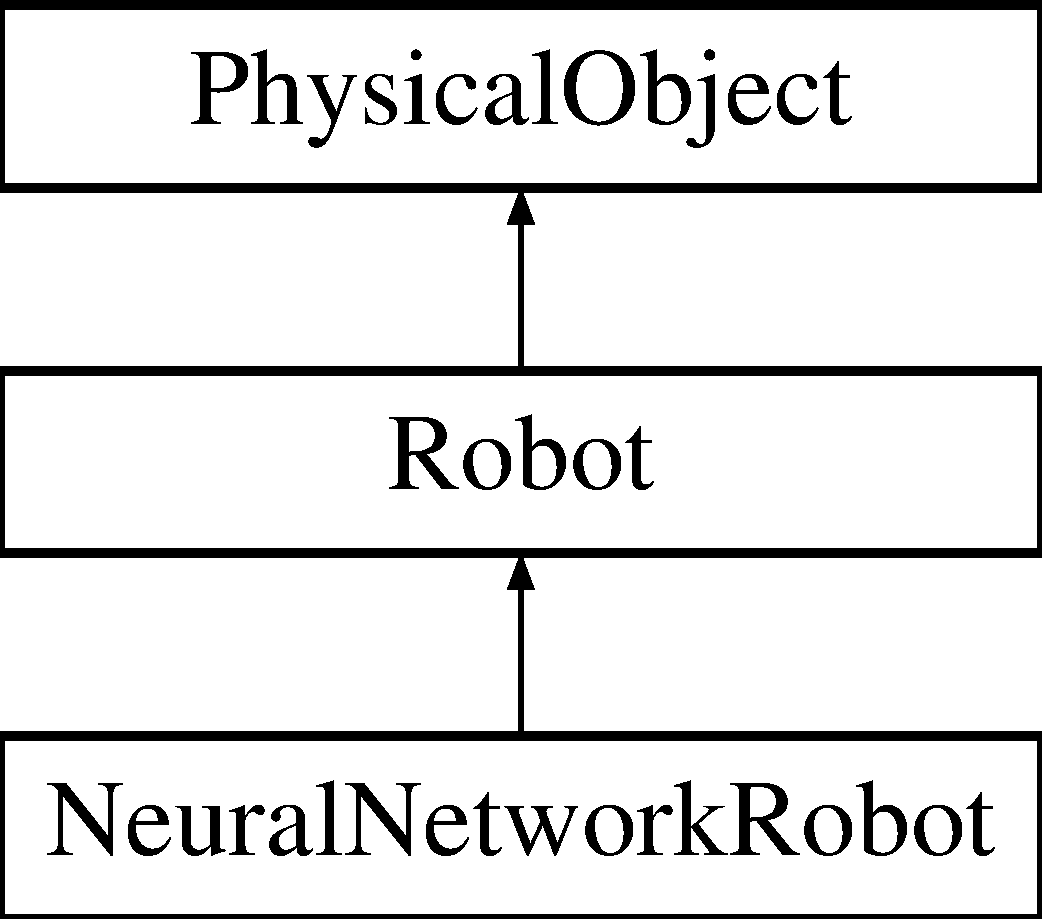
\includegraphics[height=3.000000cm]{classNeuralNetworkRobot}
\end{center}
\end{figure}
\subsection*{Public Member Functions}
\begin{DoxyCompactItemize}
\item 
\hyperlink{classNeuralNetworkRobot_adee0b00b83cd1f9269efd5178f4320b3}{Neural\-Network\-Robot} (int radius, \hyperlink{structColor}{Color} color, \hyperlink{structColor}{Color} line\-Color, \hyperlink{classNeuralNetwork}{Neural\-Network} network, int target\-Id=-\/1, std\-::string \hyperlink{classNeuralNetworkRobot_a6ccb2a3dcfa6c5616fede96f7468d065}{filename}=\hyperlink{configuration_8h_ae7f5355b60ff97037b8008b7f6d6aa74}{G\-E\-T\-\_\-\-S\-T\-R\-I\-N\-G}(\char`\"{}D\-E\-F\-A\-U\-L\-T\-\_\-\-N\-E\-U\-R\-A\-L\-\_\-\-N\-E\-T\-W\-O\-R\-K\-\_\-\-F\-I\-L\-E\char`\"{}))
\item 
\hyperlink{classNeuralNetworkRobot_a016aaca79a56d7cd2b04583188541359}{Neural\-Network\-Robot} (int radius, \hyperlink{structLocation}{Location} loc, \hyperlink{structColor}{Color} color, \hyperlink{structColor}{Color} line\-Color, \hyperlink{classNeuralNetwork}{Neural\-Network} network, int target\-Id=-\/1, std\-::string \hyperlink{classNeuralNetworkRobot_a6ccb2a3dcfa6c5616fede96f7468d065}{filename}=\hyperlink{configuration_8h_ae7f5355b60ff97037b8008b7f6d6aa74}{G\-E\-T\-\_\-\-S\-T\-R\-I\-N\-G}(\char`\"{}D\-E\-F\-A\-U\-L\-T\-\_\-\-N\-E\-U\-R\-A\-L\-\_\-\-N\-E\-T\-W\-O\-R\-K\-\_\-\-F\-I\-L\-E\char`\"{}))
\item 
\hyperlink{classNeuralNetworkRobot_a881db4125bc7390a49f0603a51a38ff1}{$\sim$\-Neural\-Network\-Robot} ()
\item 
float \hyperlink{classNeuralNetworkRobot_a91c4210b62175e9ffb1ed3362df318af}{get\-Left\-Speed} (float left\-Light\-Sensor\-Val, float right\-Light\-Sensor\-Val, float left\-Robot\-Sensor\-Val, float right\-Robot\-Sensor\-Val, float left\-Obstacle\-Sensor\-Val, float right\-Obstacle\-Sensor\-Val, float left\-Target\-Sensor\-Val, float right\-Target\-Sensor\-Val)
\item 
float \hyperlink{classNeuralNetworkRobot_a7b3389e89eb3485ad9e074494624e204}{get\-Right\-Speed} (float left\-Light\-Sensor\-Val, float right\-Light\-Sensor\-Val, float left\-Robot\-Sensor\-Val, float right\-Robot\-Sensor\-Val, float left\-Obstacle\-Sensor\-Val, float right\-Obstacle\-Sensor\-Val, float left\-Target\-Sensor\-Val, float right\-Target\-Sensor\-Val)
\end{DoxyCompactItemize}
\subsection*{Public Attributes}
\begin{DoxyCompactItemize}
\item 
const std\-::string \hyperlink{classNeuralNetworkRobot_a6ccb2a3dcfa6c5616fede96f7468d065}{filename}
\end{DoxyCompactItemize}
\subsection*{Additional Inherited Members}


\subsection{Detailed Description}
A robot controlled by a neural network with inputs from the sensors. 

\subsection{Constructor \& Destructor Documentation}
\hypertarget{classNeuralNetworkRobot_adee0b00b83cd1f9269efd5178f4320b3}{\index{Neural\-Network\-Robot@{Neural\-Network\-Robot}!Neural\-Network\-Robot@{Neural\-Network\-Robot}}
\index{Neural\-Network\-Robot@{Neural\-Network\-Robot}!NeuralNetworkRobot@{Neural\-Network\-Robot}}
\subsubsection[{Neural\-Network\-Robot}]{\setlength{\rightskip}{0pt plus 5cm}Neural\-Network\-Robot\-::\-Neural\-Network\-Robot (
\begin{DoxyParamCaption}
\item[{int}]{radius, }
\item[{{\bf Color}}]{color, }
\item[{{\bf Color}}]{line\-Color, }
\item[{{\bf Neural\-Network}}]{network, }
\item[{int}]{target\-Id = {\ttfamily -\/1}, }
\item[{std\-::string}]{filename = {\ttfamily {\bf G\-E\-T\-\_\-\-S\-T\-R\-I\-N\-G}(\char`\"{}DEFAULT\-\_\-NEURAL\-\_\-NETWORK\-\_\-FILE\char`\"{})}}
\end{DoxyParamCaption}
)}}\label{classNeuralNetworkRobot_adee0b00b83cd1f9269efd5178f4320b3}
\hypertarget{classNeuralNetworkRobot_a016aaca79a56d7cd2b04583188541359}{\index{Neural\-Network\-Robot@{Neural\-Network\-Robot}!Neural\-Network\-Robot@{Neural\-Network\-Robot}}
\index{Neural\-Network\-Robot@{Neural\-Network\-Robot}!NeuralNetworkRobot@{Neural\-Network\-Robot}}
\subsubsection[{Neural\-Network\-Robot}]{\setlength{\rightskip}{0pt plus 5cm}Neural\-Network\-Robot\-::\-Neural\-Network\-Robot (
\begin{DoxyParamCaption}
\item[{int}]{radius, }
\item[{{\bf Location}}]{loc, }
\item[{{\bf Color}}]{color, }
\item[{{\bf Color}}]{line\-Color, }
\item[{{\bf Neural\-Network}}]{network, }
\item[{int}]{target\-Id = {\ttfamily -\/1}, }
\item[{std\-::string}]{filename = {\ttfamily {\bf G\-E\-T\-\_\-\-S\-T\-R\-I\-N\-G}(\char`\"{}DEFAULT\-\_\-NEURAL\-\_\-NETWORK\-\_\-FILE\char`\"{})}}
\end{DoxyParamCaption}
)}}\label{classNeuralNetworkRobot_a016aaca79a56d7cd2b04583188541359}
\hypertarget{classNeuralNetworkRobot_a881db4125bc7390a49f0603a51a38ff1}{\index{Neural\-Network\-Robot@{Neural\-Network\-Robot}!$\sim$\-Neural\-Network\-Robot@{$\sim$\-Neural\-Network\-Robot}}
\index{$\sim$\-Neural\-Network\-Robot@{$\sim$\-Neural\-Network\-Robot}!NeuralNetworkRobot@{Neural\-Network\-Robot}}
\subsubsection[{$\sim$\-Neural\-Network\-Robot}]{\setlength{\rightskip}{0pt plus 5cm}Neural\-Network\-Robot\-::$\sim$\-Neural\-Network\-Robot (
\begin{DoxyParamCaption}
{}
\end{DoxyParamCaption}
)}}\label{classNeuralNetworkRobot_a881db4125bc7390a49f0603a51a38ff1}


\subsection{Member Function Documentation}
\hypertarget{classNeuralNetworkRobot_a91c4210b62175e9ffb1ed3362df318af}{\index{Neural\-Network\-Robot@{Neural\-Network\-Robot}!get\-Left\-Speed@{get\-Left\-Speed}}
\index{get\-Left\-Speed@{get\-Left\-Speed}!NeuralNetworkRobot@{Neural\-Network\-Robot}}
\subsubsection[{get\-Left\-Speed}]{\setlength{\rightskip}{0pt plus 5cm}float Neural\-Network\-Robot\-::get\-Left\-Speed (
\begin{DoxyParamCaption}
\item[{float}]{left\-Light\-Sensor\-Val, }
\item[{float}]{right\-Light\-Sensor\-Val, }
\item[{float}]{left\-Robot\-Sensor\-Val, }
\item[{float}]{right\-Robot\-Sensor\-Val, }
\item[{float}]{left\-Obstacle\-Sensor\-Val, }
\item[{float}]{right\-Obstacle\-Sensor\-Val, }
\item[{float}]{left\-Target\-Sensor\-Val, }
\item[{float}]{right\-Target\-Sensor\-Val}
\end{DoxyParamCaption}
)\hspace{0.3cm}{\ttfamily [virtual]}}}\label{classNeuralNetworkRobot_a91c4210b62175e9ffb1ed3362df318af}


Implements \hyperlink{classRobot_a9c96f301ae826e7c535f6b705e44bcd6}{Robot}.

\hypertarget{classNeuralNetworkRobot_a7b3389e89eb3485ad9e074494624e204}{\index{Neural\-Network\-Robot@{Neural\-Network\-Robot}!get\-Right\-Speed@{get\-Right\-Speed}}
\index{get\-Right\-Speed@{get\-Right\-Speed}!NeuralNetworkRobot@{Neural\-Network\-Robot}}
\subsubsection[{get\-Right\-Speed}]{\setlength{\rightskip}{0pt plus 5cm}float Neural\-Network\-Robot\-::get\-Right\-Speed (
\begin{DoxyParamCaption}
\item[{float}]{left\-Light\-Sensor\-Val, }
\item[{float}]{right\-Light\-Sensor\-Val, }
\item[{float}]{left\-Robot\-Sensor\-Val, }
\item[{float}]{right\-Robot\-Sensor\-Val, }
\item[{float}]{left\-Obstacle\-Sensor\-Val, }
\item[{float}]{right\-Obstacle\-Sensor\-Val, }
\item[{float}]{left\-Target\-Sensor\-Val, }
\item[{float}]{right\-Target\-Sensor\-Val}
\end{DoxyParamCaption}
)\hspace{0.3cm}{\ttfamily [virtual]}}}\label{classNeuralNetworkRobot_a7b3389e89eb3485ad9e074494624e204}


Implements \hyperlink{classRobot_a3289251979084c50b18a6006547d3f95}{Robot}.



\subsection{Member Data Documentation}
\hypertarget{classNeuralNetworkRobot_a6ccb2a3dcfa6c5616fede96f7468d065}{\index{Neural\-Network\-Robot@{Neural\-Network\-Robot}!filename@{filename}}
\index{filename@{filename}!NeuralNetworkRobot@{Neural\-Network\-Robot}}
\subsubsection[{filename}]{\setlength{\rightskip}{0pt plus 5cm}const std\-::string Neural\-Network\-Robot\-::filename}}\label{classNeuralNetworkRobot_a6ccb2a3dcfa6c5616fede96f7468d065}


The documentation for this class was generated from the following files\-:\begin{DoxyCompactItemize}
\item 
\hyperlink{NeuralNetworkRobot_8h}{Neural\-Network\-Robot.\-h}\item 
\hyperlink{NeuralNetworkRobot_8cpp}{Neural\-Network\-Robot.\-cpp}\end{DoxyCompactItemize}

\hypertarget{classNoOpenLocationException}{\section{No\-Open\-Location\-Exception Class Reference}
\label{classNoOpenLocationException}\index{No\-Open\-Location\-Exception@{No\-Open\-Location\-Exception}}
}


An exception to be thrown when an open \hyperlink{structLocation}{Location} cannot be found.  




{\ttfamily \#include $<$environment.\-h$>$}

Inheritance diagram for No\-Open\-Location\-Exception\-:\begin{figure}[H]
\begin{center}
\leavevmode
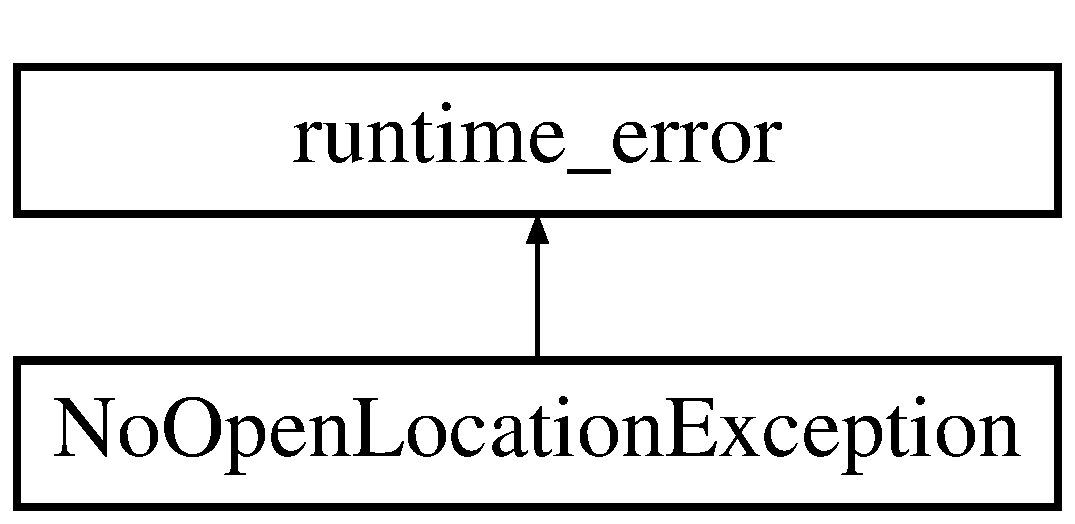
\includegraphics[height=2.000000cm]{classNoOpenLocationException}
\end{center}
\end{figure}
\subsection*{Public Member Functions}
\begin{DoxyCompactItemize}
\item 
\hyperlink{classNoOpenLocationException_afc4a5c1c30c5cd67d2e26832d2eb3738}{No\-Open\-Location\-Exception} ()
\end{DoxyCompactItemize}


\subsection{Detailed Description}
An exception to be thrown when an open \hyperlink{structLocation}{Location} cannot be found. 

\subsection{Constructor \& Destructor Documentation}
\hypertarget{classNoOpenLocationException_afc4a5c1c30c5cd67d2e26832d2eb3738}{\index{No\-Open\-Location\-Exception@{No\-Open\-Location\-Exception}!No\-Open\-Location\-Exception@{No\-Open\-Location\-Exception}}
\index{No\-Open\-Location\-Exception@{No\-Open\-Location\-Exception}!NoOpenLocationException@{No\-Open\-Location\-Exception}}
\subsubsection[{No\-Open\-Location\-Exception}]{\setlength{\rightskip}{0pt plus 5cm}No\-Open\-Location\-Exception\-::\-No\-Open\-Location\-Exception (
\begin{DoxyParamCaption}
{}
\end{DoxyParamCaption}
)\hspace{0.3cm}{\ttfamily [inline]}}}\label{classNoOpenLocationException_afc4a5c1c30c5cd67d2e26832d2eb3738}


The documentation for this class was generated from the following file\-:\begin{DoxyCompactItemize}
\item 
\hyperlink{environment_8h}{environment.\-h}\end{DoxyCompactItemize}

\hypertarget{classObjectIterator}{\section{Object\-Iterator Class Reference}
\label{classObjectIterator}\index{Object\-Iterator@{Object\-Iterator}}
}


\hyperlink{classObjectIterator}{Object\-Iterator} class, a simple iterator for the object in environment.  




{\ttfamily \#include $<$environment.\-h$>$}

\subsection*{Public Member Functions}
\begin{DoxyCompactItemize}
\item 
\hyperlink{classObjectIterator_a063765a03cce97a12c59787a1cda5121}{Object\-Iterator} ()
\begin{DoxyCompactList}\small\item\em The default constructor, the iterated objects are allways the iter\-Objects vector in environment. \end{DoxyCompactList}\item 
\hyperlink{classObjectIterator_acf20f72fa4c98e62b4a8dde10350df9f}{Object\-Iterator} (const \hyperlink{classObjectIterator}{Object\-Iterator} \&other)
\begin{DoxyCompactList}\small\item\em The copy constructor, the iterated objects are allways the iter\-Objects vector in environment. \end{DoxyCompactList}\item 
\hyperlink{classObjectIterator_a69e552a361c315f532bec9ee0bfe15a5}{$\sim$\-Object\-Iterator} ()
\begin{DoxyCompactList}\small\item\em The destructor, does nothing. \end{DoxyCompactList}\item 
void \hyperlink{classObjectIterator_aa693c5c3e5c105c6bcea5efe92ffdb22}{operator++} ()
\item 
void \hyperlink{classObjectIterator_a819be81f90fae313d20f83ee90c1057b}{operator++} (int)
\item 
\hyperlink{classPhysicalObject}{Physical\-Object} $\ast$ \hyperlink{classObjectIterator_aab94d8abe38edb14c18123a048dcd3d7}{operator$\ast$} ()
\item 
bool \hyperlink{classObjectIterator_a704f9538ed03b9c3f2c2e4a3076cac4d}{operator$>$} (const \hyperlink{classObjectIterator}{Object\-Iterator} \&other)
\item 
bool \hyperlink{classObjectIterator_a11f9437f4388b9bbc22c61663f68ec00}{operator$<$} (const \hyperlink{classObjectIterator}{Object\-Iterator} \&other)
\item 
bool \hyperlink{classObjectIterator_a7ad66f18da8432ef42eb488be531c265}{operator==} (const \hyperlink{classObjectIterator}{Object\-Iterator} \&other)
\item 
bool \hyperlink{classObjectIterator_af0b33a8a06ecb11c5c0cbfa59f40876f}{operator!=} (const \hyperlink{classObjectIterator}{Object\-Iterator} \&other)
\end{DoxyCompactItemize}
\subsection*{Friends}
\begin{DoxyCompactItemize}
\item 
\hyperlink{namespaceenvironment_a3a7a388d4b4ceb0a34bf0c72579780e1}{environment\-::object\-Iterator} \hyperlink{classObjectIterator_a90638e8c73155e7113b6c4d3fdb54c57}{environment\-::get\-Objects\-Begin} ()
\item 
\hyperlink{namespaceenvironment_a3a7a388d4b4ceb0a34bf0c72579780e1}{environment\-::object\-Iterator} \hyperlink{classObjectIterator_aede0069c558675c8d0c64d3662a42d62}{environment\-::get\-Objects\-End} ()
\end{DoxyCompactItemize}


\subsection{Detailed Description}
\hyperlink{classObjectIterator}{Object\-Iterator} class, a simple iterator for the object in environment. 

\subsection{Constructor \& Destructor Documentation}
\hypertarget{classObjectIterator_a063765a03cce97a12c59787a1cda5121}{\index{Object\-Iterator@{Object\-Iterator}!Object\-Iterator@{Object\-Iterator}}
\index{Object\-Iterator@{Object\-Iterator}!ObjectIterator@{Object\-Iterator}}
\subsubsection[{Object\-Iterator}]{\setlength{\rightskip}{0pt plus 5cm}Object\-Iterator\-::\-Object\-Iterator (
\begin{DoxyParamCaption}
{}
\end{DoxyParamCaption}
)}}\label{classObjectIterator_a063765a03cce97a12c59787a1cda5121}


The default constructor, the iterated objects are allways the iter\-Objects vector in environment. 

\hypertarget{classObjectIterator_acf20f72fa4c98e62b4a8dde10350df9f}{\index{Object\-Iterator@{Object\-Iterator}!Object\-Iterator@{Object\-Iterator}}
\index{Object\-Iterator@{Object\-Iterator}!ObjectIterator@{Object\-Iterator}}
\subsubsection[{Object\-Iterator}]{\setlength{\rightskip}{0pt plus 5cm}Object\-Iterator\-::\-Object\-Iterator (
\begin{DoxyParamCaption}
\item[{const {\bf Object\-Iterator} \&}]{other}
\end{DoxyParamCaption}
)}}\label{classObjectIterator_acf20f72fa4c98e62b4a8dde10350df9f}


The copy constructor, the iterated objects are allways the iter\-Objects vector in environment. 


\begin{DoxyParams}{Parameters}
{\em other} & The \hyperlink{classObjectIterator}{Object\-Iterator} to copy \\
\hline
\end{DoxyParams}
\hypertarget{classObjectIterator_a69e552a361c315f532bec9ee0bfe15a5}{\index{Object\-Iterator@{Object\-Iterator}!$\sim$\-Object\-Iterator@{$\sim$\-Object\-Iterator}}
\index{$\sim$\-Object\-Iterator@{$\sim$\-Object\-Iterator}!ObjectIterator@{Object\-Iterator}}
\subsubsection[{$\sim$\-Object\-Iterator}]{\setlength{\rightskip}{0pt plus 5cm}Object\-Iterator\-::$\sim$\-Object\-Iterator (
\begin{DoxyParamCaption}
{}
\end{DoxyParamCaption}
)}}\label{classObjectIterator_a69e552a361c315f532bec9ee0bfe15a5}


The destructor, does nothing. 



\subsection{Member Function Documentation}
\hypertarget{classObjectIterator_af0b33a8a06ecb11c5c0cbfa59f40876f}{\index{Object\-Iterator@{Object\-Iterator}!operator!=@{operator!=}}
\index{operator!=@{operator!=}!ObjectIterator@{Object\-Iterator}}
\subsubsection[{operator!=}]{\setlength{\rightskip}{0pt plus 5cm}bool Object\-Iterator\-::operator!= (
\begin{DoxyParamCaption}
\item[{const {\bf Object\-Iterator} \&}]{other}
\end{DoxyParamCaption}
)}}\label{classObjectIterator_af0b33a8a06ecb11c5c0cbfa59f40876f}
\hypertarget{classObjectIterator_aab94d8abe38edb14c18123a048dcd3d7}{\index{Object\-Iterator@{Object\-Iterator}!operator$\ast$@{operator$\ast$}}
\index{operator$\ast$@{operator$\ast$}!ObjectIterator@{Object\-Iterator}}
\subsubsection[{operator$\ast$}]{\setlength{\rightskip}{0pt plus 5cm}{\bf Physical\-Object} $\ast$ Object\-Iterator\-::operator$\ast$ (
\begin{DoxyParamCaption}
{}
\end{DoxyParamCaption}
)}}\label{classObjectIterator_aab94d8abe38edb14c18123a048dcd3d7}
\hypertarget{classObjectIterator_aa693c5c3e5c105c6bcea5efe92ffdb22}{\index{Object\-Iterator@{Object\-Iterator}!operator++@{operator++}}
\index{operator++@{operator++}!ObjectIterator@{Object\-Iterator}}
\subsubsection[{operator++}]{\setlength{\rightskip}{0pt plus 5cm}void Object\-Iterator\-::operator++ (
\begin{DoxyParamCaption}
{}
\end{DoxyParamCaption}
)}}\label{classObjectIterator_aa693c5c3e5c105c6bcea5efe92ffdb22}
\hypertarget{classObjectIterator_a819be81f90fae313d20f83ee90c1057b}{\index{Object\-Iterator@{Object\-Iterator}!operator++@{operator++}}
\index{operator++@{operator++}!ObjectIterator@{Object\-Iterator}}
\subsubsection[{operator++}]{\setlength{\rightskip}{0pt plus 5cm}void Object\-Iterator\-::operator++ (
\begin{DoxyParamCaption}
\item[{int}]{}
\end{DoxyParamCaption}
)}}\label{classObjectIterator_a819be81f90fae313d20f83ee90c1057b}
\hypertarget{classObjectIterator_a11f9437f4388b9bbc22c61663f68ec00}{\index{Object\-Iterator@{Object\-Iterator}!operator$<$@{operator$<$}}
\index{operator$<$@{operator$<$}!ObjectIterator@{Object\-Iterator}}
\subsubsection[{operator$<$}]{\setlength{\rightskip}{0pt plus 5cm}bool Object\-Iterator\-::operator$<$ (
\begin{DoxyParamCaption}
\item[{const {\bf Object\-Iterator} \&}]{other}
\end{DoxyParamCaption}
)}}\label{classObjectIterator_a11f9437f4388b9bbc22c61663f68ec00}
\hypertarget{classObjectIterator_a7ad66f18da8432ef42eb488be531c265}{\index{Object\-Iterator@{Object\-Iterator}!operator==@{operator==}}
\index{operator==@{operator==}!ObjectIterator@{Object\-Iterator}}
\subsubsection[{operator==}]{\setlength{\rightskip}{0pt plus 5cm}bool Object\-Iterator\-::operator== (
\begin{DoxyParamCaption}
\item[{const {\bf Object\-Iterator} \&}]{other}
\end{DoxyParamCaption}
)}}\label{classObjectIterator_a7ad66f18da8432ef42eb488be531c265}
\hypertarget{classObjectIterator_a704f9538ed03b9c3f2c2e4a3076cac4d}{\index{Object\-Iterator@{Object\-Iterator}!operator$>$@{operator$>$}}
\index{operator$>$@{operator$>$}!ObjectIterator@{Object\-Iterator}}
\subsubsection[{operator$>$}]{\setlength{\rightskip}{0pt plus 5cm}bool Object\-Iterator\-::operator$>$ (
\begin{DoxyParamCaption}
\item[{const {\bf Object\-Iterator} \&}]{other}
\end{DoxyParamCaption}
)}}\label{classObjectIterator_a704f9538ed03b9c3f2c2e4a3076cac4d}


\subsection{Friends And Related Function Documentation}
\hypertarget{classObjectIterator_a90638e8c73155e7113b6c4d3fdb54c57}{\index{Object\-Iterator@{Object\-Iterator}!environment\-::get\-Objects\-Begin@{environment\-::get\-Objects\-Begin}}
\index{environment\-::get\-Objects\-Begin@{environment\-::get\-Objects\-Begin}!ObjectIterator@{Object\-Iterator}}
\subsubsection[{environment\-::get\-Objects\-Begin}]{\setlength{\rightskip}{0pt plus 5cm}{\bf environment\-::object\-Iterator} {\bf environment\-::get\-Objects\-Begin} (
\begin{DoxyParamCaption}
{}
\end{DoxyParamCaption}
)\hspace{0.3cm}{\ttfamily [friend]}}}\label{classObjectIterator_a90638e8c73155e7113b6c4d3fdb54c57}
\hypertarget{classObjectIterator_aede0069c558675c8d0c64d3662a42d62}{\index{Object\-Iterator@{Object\-Iterator}!environment\-::get\-Objects\-End@{environment\-::get\-Objects\-End}}
\index{environment\-::get\-Objects\-End@{environment\-::get\-Objects\-End}!ObjectIterator@{Object\-Iterator}}
\subsubsection[{environment\-::get\-Objects\-End}]{\setlength{\rightskip}{0pt plus 5cm}{\bf environment\-::object\-Iterator} {\bf environment\-::get\-Objects\-End} (
\begin{DoxyParamCaption}
{}
\end{DoxyParamCaption}
)\hspace{0.3cm}{\ttfamily [friend]}}}\label{classObjectIterator_aede0069c558675c8d0c64d3662a42d62}


The documentation for this class was generated from the following files\-:\begin{DoxyCompactItemize}
\item 
\hyperlink{environment_8h}{environment.\-h}\item 
\hyperlink{environment_8cpp}{environment.\-cpp}\end{DoxyCompactItemize}

\hypertarget{classObstacle}{\section{Obstacle Class Reference}
\label{classObstacle}\index{Obstacle@{Obstacle}}
}


\hyperlink{classObstacle}{Obstacle} for the robot to hit/avoid.  




{\ttfamily \#include $<$Obstacle.\-h$>$}

Inheritance diagram for Obstacle\-:\begin{figure}[H]
\begin{center}
\leavevmode
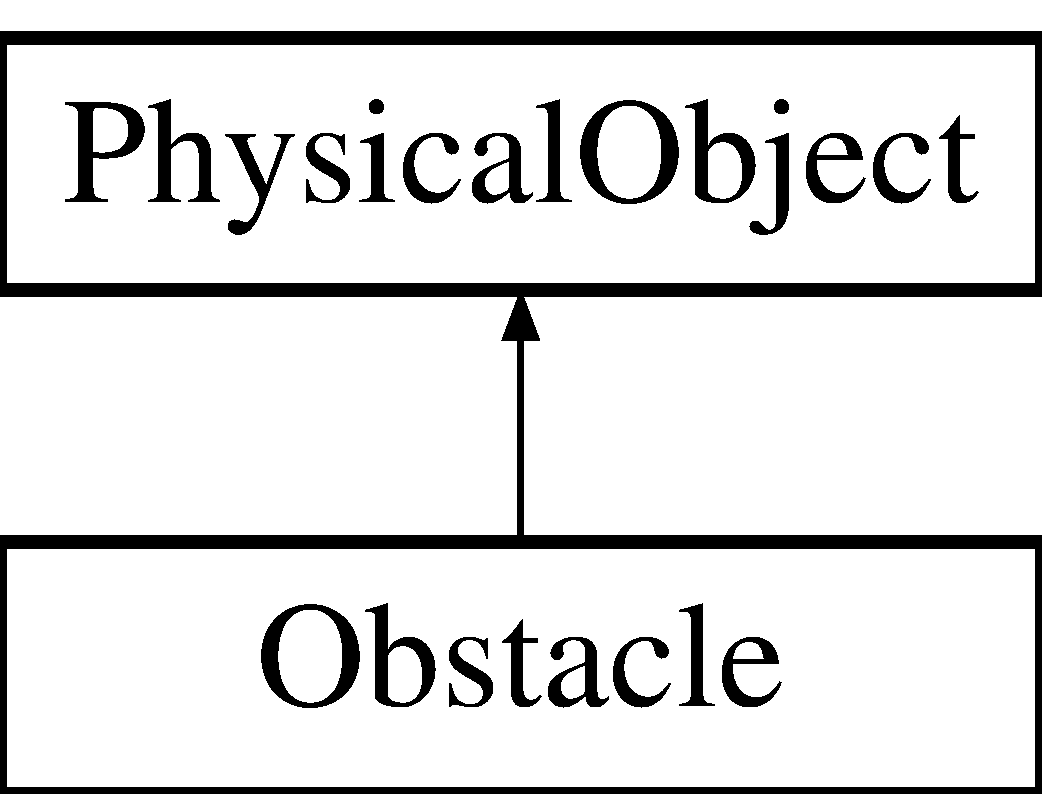
\includegraphics[height=2.000000cm]{classObstacle}
\end{center}
\end{figure}
\subsection*{Public Member Functions}
\begin{DoxyCompactItemize}
\item 
\hyperlink{classObstacle_a05684b15f4ea925bd64601e534650ce7}{Obstacle} (int radius, \hyperlink{structColor}{Color} color)
\item 
\hyperlink{classObstacle_ae4f3c942fab622b38e32f1c2514f0924}{Obstacle} (int max\-Radius, int min\-Radius, \hyperlink{structColor}{Color} color)
\item 
\hyperlink{classObstacle_a28e78317f4f4b06fb6acec5a75f918c4}{Obstacle} (int radius, \hyperlink{structLocation}{Location} loc, \hyperlink{structColor}{Color} color)
\item 
bool \hyperlink{classObstacle_a6ea72857ac6d643be7bb3bd3a1a30995}{handle\-Collision} (int other\-Id, bool was\-Hit)
\item 
\hyperlink{classObstacle_af2f9cc9c6cff75dca0974fd5ac4f71a9}{$\sim$\-Obstacle} ()
\end{DoxyCompactItemize}
\subsection*{Additional Inherited Members}


\subsection{Detailed Description}
\hyperlink{classObstacle}{Obstacle} for the robot to hit/avoid. 

\subsection{Constructor \& Destructor Documentation}
\hypertarget{classObstacle_a05684b15f4ea925bd64601e534650ce7}{\index{Obstacle@{Obstacle}!Obstacle@{Obstacle}}
\index{Obstacle@{Obstacle}!Obstacle@{Obstacle}}
\subsubsection[{Obstacle}]{\setlength{\rightskip}{0pt plus 5cm}Obstacle\-::\-Obstacle (
\begin{DoxyParamCaption}
\item[{int}]{radius, }
\item[{{\bf Color}}]{color}
\end{DoxyParamCaption}
)}}\label{classObstacle_a05684b15f4ea925bd64601e534650ce7}

\begin{DoxyParams}{Parameters}
{\em radius} & the radius in pixels \\
\hline
{\em color} & a struct of float value 0 to 1 representing a hexedecimal color \\
\hline
{\em config} & a configuration table \\
\hline
\end{DoxyParams}
\begin{DoxyParagraph}{Initialization}
\hyperlink{classObstacle}{Obstacle} is initialized with the following values\-: 
\end{DoxyParagraph}


Radius\-: D\-E\-F\-A\-U\-L\-T\-\_\-\-R\-A\-D\-I\-U\-S as specified in ../config/default  

Orientation\-: random 

Speed\-: 0 

Position\-: (loc.\-x, loc.\-y)   \hypertarget{classObstacle_ae4f3c942fab622b38e32f1c2514f0924}{\index{Obstacle@{Obstacle}!Obstacle@{Obstacle}}
\index{Obstacle@{Obstacle}!Obstacle@{Obstacle}}
\subsubsection[{Obstacle}]{\setlength{\rightskip}{0pt plus 5cm}Obstacle\-::\-Obstacle (
\begin{DoxyParamCaption}
\item[{int}]{max\-Radius, }
\item[{int}]{min\-Radius, }
\item[{{\bf Color}}]{color}
\end{DoxyParamCaption}
)}}\label{classObstacle_ae4f3c942fab622b38e32f1c2514f0924}

\begin{DoxyParams}{Parameters}
{\em min\-Radius} & the minimum radius in pixels \\
\hline
{\em max\-Radius} & the maximum radius in pixels \\
\hline
{\em color} & a struct of float value 0 to 1 representing a hexedecimal color \\
\hline
\end{DoxyParams}
\begin{DoxyParagraph}{Initialization}
\hyperlink{classObstacle}{Obstacle} is initialized with the following values\-: 
\end{DoxyParagraph}


Orientation\-: random 

Speed\-: 0 

Position\-: (loc.\-x, loc.\-y)   \hypertarget{classObstacle_a28e78317f4f4b06fb6acec5a75f918c4}{\index{Obstacle@{Obstacle}!Obstacle@{Obstacle}}
\index{Obstacle@{Obstacle}!Obstacle@{Obstacle}}
\subsubsection[{Obstacle}]{\setlength{\rightskip}{0pt plus 5cm}Obstacle\-::\-Obstacle (
\begin{DoxyParamCaption}
\item[{int}]{radius, }
\item[{{\bf Location}}]{loc, }
\item[{{\bf Color}}]{color}
\end{DoxyParamCaption}
)}}\label{classObstacle_a28e78317f4f4b06fb6acec5a75f918c4}

\begin{DoxyParams}{Parameters}
{\em radius} & the radius in pixels \\
\hline
{\em color} & a struct of float value 0 to 1 representing a hexedecimal color \\
\hline
{\em loc} & a struct of the x,y start \hyperlink{structLocation}{Location} in pixels \\
\hline
\end{DoxyParams}
\begin{DoxyParagraph}{Initialization}
\hyperlink{classObstacle}{Obstacle} is initialized with the following values\-: 
\end{DoxyParagraph}


Orientation\-: 0 

Speed\-: 0 

Position\-: (loc.\-x, loc.\-y)   \hypertarget{classObstacle_af2f9cc9c6cff75dca0974fd5ac4f71a9}{\index{Obstacle@{Obstacle}!$\sim$\-Obstacle@{$\sim$\-Obstacle}}
\index{$\sim$\-Obstacle@{$\sim$\-Obstacle}!Obstacle@{Obstacle}}
\subsubsection[{$\sim$\-Obstacle}]{\setlength{\rightskip}{0pt plus 5cm}Obstacle\-::$\sim$\-Obstacle (
\begin{DoxyParamCaption}
{}
\end{DoxyParamCaption}
)}}\label{classObstacle_af2f9cc9c6cff75dca0974fd5ac4f71a9}
This is the class destructor. 

\subsection{Member Function Documentation}
\hypertarget{classObstacle_a6ea72857ac6d643be7bb3bd3a1a30995}{\index{Obstacle@{Obstacle}!handle\-Collision@{handle\-Collision}}
\index{handle\-Collision@{handle\-Collision}!Obstacle@{Obstacle}}
\subsubsection[{handle\-Collision}]{\setlength{\rightskip}{0pt plus 5cm}bool Obstacle\-::handle\-Collision (
\begin{DoxyParamCaption}
\item[{int}]{other\-Id, }
\item[{bool}]{was\-Hit}
\end{DoxyParamCaption}
)\hspace{0.3cm}{\ttfamily [virtual]}}}\label{classObstacle_a6ea72857ac6d643be7bb3bd3a1a30995}
\begin{DoxyAuthor}{Author}
Lucas Kramer This function gives \hyperlink{classObstacle}{Obstacle} an appropriate reaction when a collision occurs. Does nothing for now 
\end{DoxyAuthor}

\begin{DoxyParams}{Parameters}
{\em other\-Id} & id of the object that it collides with \\
\hline
{\em was\-Hit} & tells if the object was hit previously \\
\hline
\end{DoxyParams}


Implements \hyperlink{classPhysicalObject_a400ba3545479ebbf8b1b4a046906e562}{Physical\-Object}.



The documentation for this class was generated from the following files\-:\begin{DoxyCompactItemize}
\item 
\hyperlink{Obstacle_8h}{Obstacle.\-h}\item 
\hyperlink{Obstacle_8cpp}{Obstacle.\-cpp}\end{DoxyCompactItemize}

\hypertarget{classOptimizeSimulation}{\section{Optimize\-Simulation Class Reference}
\label{classOptimizeSimulation}\index{Optimize\-Simulation@{Optimize\-Simulation}}
}


\hyperlink{classOptimizeSimulation}{Optimize\-Simulation} class, sets up environments and robots.  




{\ttfamily \#include $<$Optimize\-Simulation.\-h$>$}

\subsection*{Public Member Functions}
\begin{DoxyCompactItemize}
\item 
\hyperlink{classOptimizeSimulation_a24503060026d2f4bb2224e6ba3f554a5}{Optimize\-Simulation} (int argc, char $\ast$argv\mbox{[}$\,$\mbox{]})
\begin{DoxyCompactList}\small\item\em The constructor for the \hyperlink{classSimulation}{Simulation} class. \end{DoxyCompactList}\item 
virtual \hyperlink{classOptimizeSimulation_a4c097b55978ea713789ea1f4b97630e1}{$\sim$\-Optimize\-Simulation} ()
\item 
void \hyperlink{classOptimizeSimulation_a51f48566cb982a61daa877d213c528b0}{run\-Main\-Loop} ()
\item 
void \hyperlink{classOptimizeSimulation_a0216d870b6d411e771424be041658d36}{stop} ()
\item 
int \hyperlink{classOptimizeSimulation_af14f1d43b9c80f3a3121bd62a133ce28}{get\-Performance} (const \hyperlink{classNeuralNetwork}{Neural\-Network} \&network)
\item 
int \hyperlink{classOptimizeSimulation_ace9c1e57f259d3e69aa1fbd8d971985c}{get\-Performance\-Random\-Repeated} (const \hyperlink{classNeuralNetwork}{Neural\-Network} \&network)
\item 
int \hyperlink{classOptimizeSimulation_ab2d721222b5dc4a2831d70af136409e7}{get\-Performance\-Maze} (const \hyperlink{classNeuralNetwork}{Neural\-Network} \&network)
\item 
int \hyperlink{classOptimizeSimulation_a27f0912295edf0a54e4251bb17291bba}{get\-Performance\-Obstacles} (const \hyperlink{classNeuralNetwork}{Neural\-Network} \&network)
\end{DoxyCompactItemize}


\subsection{Detailed Description}
\hyperlink{classOptimizeSimulation}{Optimize\-Simulation} class, sets up environments and robots. 

\subsection{Constructor \& Destructor Documentation}
\hypertarget{classOptimizeSimulation_a24503060026d2f4bb2224e6ba3f554a5}{\index{Optimize\-Simulation@{Optimize\-Simulation}!Optimize\-Simulation@{Optimize\-Simulation}}
\index{Optimize\-Simulation@{Optimize\-Simulation}!OptimizeSimulation@{Optimize\-Simulation}}
\subsubsection[{Optimize\-Simulation}]{\setlength{\rightskip}{0pt plus 5cm}Optimize\-Simulation\-::\-Optimize\-Simulation (
\begin{DoxyParamCaption}
\item[{int}]{argc, }
\item[{char $\ast$}]{argv\mbox{[}$\,$\mbox{]}}
\end{DoxyParamCaption}
)}}\label{classOptimizeSimulation_a24503060026d2f4bb2224e6ba3f554a5}


The constructor for the \hyperlink{classSimulation}{Simulation} class. 


\begin{DoxyParams}{Parameters}
{\em argc} & The number of command-\/line arguments \\
\hline
{\em argv} & The command-\/line arguments \\
\hline
\end{DoxyParams}
\hypertarget{classOptimizeSimulation_a4c097b55978ea713789ea1f4b97630e1}{\index{Optimize\-Simulation@{Optimize\-Simulation}!$\sim$\-Optimize\-Simulation@{$\sim$\-Optimize\-Simulation}}
\index{$\sim$\-Optimize\-Simulation@{$\sim$\-Optimize\-Simulation}!OptimizeSimulation@{Optimize\-Simulation}}
\subsubsection[{$\sim$\-Optimize\-Simulation}]{\setlength{\rightskip}{0pt plus 5cm}Optimize\-Simulation\-::$\sim$\-Optimize\-Simulation (
\begin{DoxyParamCaption}
{}
\end{DoxyParamCaption}
)\hspace{0.3cm}{\ttfamily [virtual]}}}\label{classOptimizeSimulation_a4c097b55978ea713789ea1f4b97630e1}


\subsection{Member Function Documentation}
\hypertarget{classOptimizeSimulation_af14f1d43b9c80f3a3121bd62a133ce28}{\index{Optimize\-Simulation@{Optimize\-Simulation}!get\-Performance@{get\-Performance}}
\index{get\-Performance@{get\-Performance}!OptimizeSimulation@{Optimize\-Simulation}}
\subsubsection[{get\-Performance}]{\setlength{\rightskip}{0pt plus 5cm}int Optimize\-Simulation\-::get\-Performance (
\begin{DoxyParamCaption}
\item[{const {\bf Neural\-Network} \&}]{network}
\end{DoxyParamCaption}
)}}\label{classOptimizeSimulation_af14f1d43b9c80f3a3121bd62a133ce28}
\hypertarget{classOptimizeSimulation_ab2d721222b5dc4a2831d70af136409e7}{\index{Optimize\-Simulation@{Optimize\-Simulation}!get\-Performance\-Maze@{get\-Performance\-Maze}}
\index{get\-Performance\-Maze@{get\-Performance\-Maze}!OptimizeSimulation@{Optimize\-Simulation}}
\subsubsection[{get\-Performance\-Maze}]{\setlength{\rightskip}{0pt plus 5cm}int Optimize\-Simulation\-::get\-Performance\-Maze (
\begin{DoxyParamCaption}
\item[{const {\bf Neural\-Network} \&}]{network}
\end{DoxyParamCaption}
)}}\label{classOptimizeSimulation_ab2d721222b5dc4a2831d70af136409e7}
\hypertarget{classOptimizeSimulation_a27f0912295edf0a54e4251bb17291bba}{\index{Optimize\-Simulation@{Optimize\-Simulation}!get\-Performance\-Obstacles@{get\-Performance\-Obstacles}}
\index{get\-Performance\-Obstacles@{get\-Performance\-Obstacles}!OptimizeSimulation@{Optimize\-Simulation}}
\subsubsection[{get\-Performance\-Obstacles}]{\setlength{\rightskip}{0pt plus 5cm}int Optimize\-Simulation\-::get\-Performance\-Obstacles (
\begin{DoxyParamCaption}
\item[{const {\bf Neural\-Network} \&}]{network}
\end{DoxyParamCaption}
)}}\label{classOptimizeSimulation_a27f0912295edf0a54e4251bb17291bba}
\hypertarget{classOptimizeSimulation_ace9c1e57f259d3e69aa1fbd8d971985c}{\index{Optimize\-Simulation@{Optimize\-Simulation}!get\-Performance\-Random\-Repeated@{get\-Performance\-Random\-Repeated}}
\index{get\-Performance\-Random\-Repeated@{get\-Performance\-Random\-Repeated}!OptimizeSimulation@{Optimize\-Simulation}}
\subsubsection[{get\-Performance\-Random\-Repeated}]{\setlength{\rightskip}{0pt plus 5cm}int Optimize\-Simulation\-::get\-Performance\-Random\-Repeated (
\begin{DoxyParamCaption}
\item[{const {\bf Neural\-Network} \&}]{network}
\end{DoxyParamCaption}
)}}\label{classOptimizeSimulation_ace9c1e57f259d3e69aa1fbd8d971985c}
\hypertarget{classOptimizeSimulation_a51f48566cb982a61daa877d213c528b0}{\index{Optimize\-Simulation@{Optimize\-Simulation}!run\-Main\-Loop@{run\-Main\-Loop}}
\index{run\-Main\-Loop@{run\-Main\-Loop}!OptimizeSimulation@{Optimize\-Simulation}}
\subsubsection[{run\-Main\-Loop}]{\setlength{\rightskip}{0pt plus 5cm}void Optimize\-Simulation\-::run\-Main\-Loop (
\begin{DoxyParamCaption}
{}
\end{DoxyParamCaption}
)}}\label{classOptimizeSimulation_a51f48566cb982a61daa877d213c528b0}
\hypertarget{classOptimizeSimulation_a0216d870b6d411e771424be041658d36}{\index{Optimize\-Simulation@{Optimize\-Simulation}!stop@{stop}}
\index{stop@{stop}!OptimizeSimulation@{Optimize\-Simulation}}
\subsubsection[{stop}]{\setlength{\rightskip}{0pt plus 5cm}void Optimize\-Simulation\-::stop (
\begin{DoxyParamCaption}
{}
\end{DoxyParamCaption}
)}}\label{classOptimizeSimulation_a0216d870b6d411e771424be041658d36}


The documentation for this class was generated from the following files\-:\begin{DoxyCompactItemize}
\item 
\hyperlink{OptimizeSimulation_8h}{Optimize\-Simulation.\-h}\item 
\hyperlink{OptimizeSimulation_8cpp}{Optimize\-Simulation.\-cpp}\end{DoxyCompactItemize}

\hypertarget{classPhysicalObject}{\section{Physical\-Object Class Reference}
\label{classPhysicalObject}\index{Physical\-Object@{Physical\-Object}}
}


This is a common superclass for all objects.  




{\ttfamily \#include $<$Physical\-Object.\-h$>$}

Inheritance diagram for Physical\-Object\-:\begin{figure}[H]
\begin{center}
\leavevmode
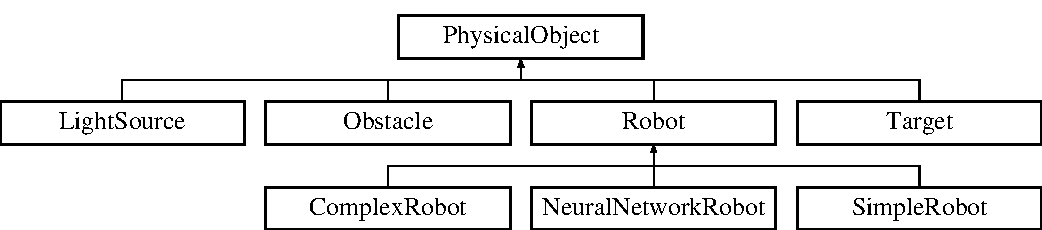
\includegraphics[height=3.000000cm]{classPhysicalObject}
\end{center}
\end{figure}
\subsection*{Public Member Functions}
\begin{DoxyCompactItemize}
\item 
\hyperlink{classPhysicalObject_a2fbf277629a4b9dec946be7241d034f4}{Physical\-Object} (\hyperlink{PhysicalObject_8h_a842c5e2e69277690b064bf363c017980}{Object\-Type} \hyperlink{classPhysicalObject_a59060233e54004b24fc03ed786b46dd3}{object\-Type}, int radius=G\-E\-T\-\_\-\-I\-N\-T(\char`\"{}D\-E\-F\-A\-U\-L\-T\-\_\-\-R\-A\-D\-I\-U\-S\char`\"{}), Color color=\hyperlink{structColor}{Color}('?'), bool \hyperlink{classPhysicalObject_a5afc803dac6415f86fcda81983b75e41}{is\-Hitable}=true)
\item 
\hyperlink{classPhysicalObject_a9a132760e19b893b51deb542dc53a859}{Physical\-Object} (\hyperlink{PhysicalObject_8h_a842c5e2e69277690b064bf363c017980}{Object\-Type} \hyperlink{classPhysicalObject_a59060233e54004b24fc03ed786b46dd3}{object\-Type}, int max\-Radius, int min\-Radius, \hyperlink{structColor}{Color} color=\hyperlink{structColor}{Color}('?'), bool \hyperlink{classPhysicalObject_a5afc803dac6415f86fcda81983b75e41}{is\-Hitable}=true)
\item 
\hyperlink{classPhysicalObject_afc9f843a4c6083587ce2e20a091d0a79}{Physical\-Object} (\hyperlink{PhysicalObject_8h_a842c5e2e69277690b064bf363c017980}{Object\-Type} \hyperlink{classPhysicalObject_a59060233e54004b24fc03ed786b46dd3}{object\-Type}, int radius, \hyperlink{structLocation}{Location} loc, \hyperlink{structColor}{Color} color=\hyperlink{structColor}{Color}('?'), bool \hyperlink{classPhysicalObject_a5afc803dac6415f86fcda81983b75e41}{is\-Hitable}=true)
\item 
virtual \hyperlink{classPhysicalObject_a473fb6a285d967b295e4c700c341afe4}{$\sim$\-Physical\-Object} ()
\item 
int \hyperlink{classPhysicalObject_a71514ab30d4543a2720fd4ac0f3f6401}{get\-Id} () const 
\item 
void \hyperlink{classPhysicalObject_ac130b3a86fa816eee60783e0120b7d98}{set\-Position} (float x, float y)
\item 
void \hyperlink{classPhysicalObject_a9c562fb0b7e468d4b6d9a1a429791236}{force\-Set\-Position} (float x, float y)
\item 
void \hyperlink{classPhysicalObject_a0ffd9a9890787fdcfe31ebbf2931aff5}{set\-Location} (\hyperlink{structLocation}{Location} loc)
\item 
void \hyperlink{classPhysicalObject_a6e580010f7b025beacdee13835c8a726}{reorient} (int angle, float distance)
\item 
bool \hyperlink{classPhysicalObject_a2246c1f65d47638f61c2996d477efc6f}{translate} (float distance)
\item 
void \hyperlink{classPhysicalObject_a7121bd6642a98adc38e8c3348c4a3e01}{force\-Translate} (float distance)
\item 
void \hyperlink{classPhysicalObject_ac78eb70d7b7d24a586e5eed347f3a8d2}{set\-Orientation} (int degrees)
\item 
void \hyperlink{classPhysicalObject_ae197cc719763a64d34fc9723458aab01}{set\-Speed} (int pps)
\item 
void \hyperlink{classPhysicalObject_a81be6f4317d6813ab0b73ccf00da181a}{set\-Radius} (int radius)
\item 
void \hyperlink{classPhysicalObject_a2f5bff48537b44f6f1abd4500c644bc8}{set\-Color} (\hyperlink{structColor}{Color} color)
\item 
float \hyperlink{classPhysicalObject_a37bacbedf0b90865403149a1396ee58f}{get\-X\-Position} () const 
\item 
float \hyperlink{classPhysicalObject_a95b02cbe019cc2f968eb482487b5db7e}{get\-Y\-Position} () const 
\item 
\hyperlink{structLocation}{Location} \hyperlink{classPhysicalObject_a92b2b2addc7f85396c19fc255393e558}{get\-Location} () const 
\item 
int \hyperlink{classPhysicalObject_ac6d9bb140bcf0e492a0792e3eadbb3a8}{get\-Orientation} () const 
\item 
int \hyperlink{classPhysicalObject_a1f687df65cf05bed55a43edfda87790d}{get\-Speed} () const 
\item 
int \hyperlink{classPhysicalObject_a311d08aaa4bc7c863d0349397b187e6c}{get\-Radius} () const 
\item 
\hyperlink{structColor}{Color} \hyperlink{classPhysicalObject_aad8e15d2bec5e7c4fd38c2a8335dc0a0}{get\-Color} () const 
\item 
void \hyperlink{classPhysicalObject_aa4e04a3becfa1be5b3fea856a2f0c3fb}{point\-To} (const \hyperlink{classPhysicalObject}{Physical\-Object} \&other)
\item 
void \hyperlink{classPhysicalObject_abb08525b7fa5fa7f3b936847c28bb630}{rotate} (int degrees)
\item 
bool \hyperlink{classPhysicalObject_a2bfa9e53acb308cdbfdda0945a8b1fe3}{has\-Equal\-Position} (const \hyperlink{classPhysicalObject}{Physical\-Object} \&other) const 
\item 
bool \hyperlink{classPhysicalObject_a5e2b241c127b7114693736f89cafc9fb}{update\-Position} ()
\item 
virtual void \hyperlink{classPhysicalObject_a3005ac0afce838049101db17525f6004}{update} ()
\item 
virtual void \hyperlink{classPhysicalObject_a4fc8c0c62b8e12a63ebdf13136d577ac}{update\-Members} ()
\item 
virtual void \hyperlink{classPhysicalObject_a6a0326df3efc0a1ea23892e3fcd4b11e}{display} ()
\item 
virtual bool \hyperlink{classPhysicalObject_a400ba3545479ebbf8b1b4a046906e562}{handle\-Collision} (int other\-Id, bool was\-Hit)=0
\end{DoxyCompactItemize}
\subsection*{Public Attributes}
\begin{DoxyCompactItemize}
\item 
const \hyperlink{PhysicalObject_8h_a842c5e2e69277690b064bf363c017980}{Object\-Type} \hyperlink{classPhysicalObject_a59060233e54004b24fc03ed786b46dd3}{object\-Type}
\item 
const bool \hyperlink{classPhysicalObject_a5afc803dac6415f86fcda81983b75e41}{is\-Hitable}
\end{DoxyCompactItemize}
\subsection*{Static Protected Member Functions}
\begin{DoxyCompactItemize}
\item 
static \hyperlink{structLocation}{Location} \hyperlink{classPhysicalObject_ae184c1c797f3dd8786ca266019a6f283}{find\-Open\-Location} (int radius)
\end{DoxyCompactItemize}


\subsection{Detailed Description}
This is a common superclass for all objects. 

\subsection{Constructor \& Destructor Documentation}
\hypertarget{classPhysicalObject_a2fbf277629a4b9dec946be7241d034f4}{\index{Physical\-Object@{Physical\-Object}!Physical\-Object@{Physical\-Object}}
\index{Physical\-Object@{Physical\-Object}!PhysicalObject@{Physical\-Object}}
\subsubsection[{Physical\-Object}]{\setlength{\rightskip}{0pt plus 5cm}Physical\-Object\-::\-Physical\-Object (
\begin{DoxyParamCaption}
\item[{{\bf Object\-Type}}]{object\-Type, }
\item[{int}]{radius = {\ttfamily GET\-\_\-INT(\char`\"{}DEFAULT\-\_\-RADIUS\char`\"{})}, }
\item[{{\bf Color}}]{color = {\ttfamily {\bf Color}('?')}, }
\item[{bool}]{is\-Hitable = {\ttfamily true}}
\end{DoxyParamCaption}
)}}\label{classPhysicalObject_a2fbf277629a4b9dec946be7241d034f4}
\hypertarget{classPhysicalObject_a9a132760e19b893b51deb542dc53a859}{\index{Physical\-Object@{Physical\-Object}!Physical\-Object@{Physical\-Object}}
\index{Physical\-Object@{Physical\-Object}!PhysicalObject@{Physical\-Object}}
\subsubsection[{Physical\-Object}]{\setlength{\rightskip}{0pt plus 5cm}Physical\-Object\-::\-Physical\-Object (
\begin{DoxyParamCaption}
\item[{{\bf Object\-Type}}]{object\-Type, }
\item[{int}]{max\-Radius, }
\item[{int}]{min\-Radius, }
\item[{{\bf Color}}]{color = {\ttfamily {\bf Color}('?')}, }
\item[{bool}]{is\-Hitable = {\ttfamily true}}
\end{DoxyParamCaption}
)}}\label{classPhysicalObject_a9a132760e19b893b51deb542dc53a859}
\hypertarget{classPhysicalObject_afc9f843a4c6083587ce2e20a091d0a79}{\index{Physical\-Object@{Physical\-Object}!Physical\-Object@{Physical\-Object}}
\index{Physical\-Object@{Physical\-Object}!PhysicalObject@{Physical\-Object}}
\subsubsection[{Physical\-Object}]{\setlength{\rightskip}{0pt plus 5cm}Physical\-Object\-::\-Physical\-Object (
\begin{DoxyParamCaption}
\item[{{\bf Object\-Type}}]{object\-Type, }
\item[{int}]{radius, }
\item[{{\bf Location}}]{loc, }
\item[{{\bf Color}}]{color = {\ttfamily {\bf Color}('?')}, }
\item[{bool}]{is\-Hitable = {\ttfamily true}}
\end{DoxyParamCaption}
)}}\label{classPhysicalObject_afc9f843a4c6083587ce2e20a091d0a79}
\hypertarget{classPhysicalObject_a473fb6a285d967b295e4c700c341afe4}{\index{Physical\-Object@{Physical\-Object}!$\sim$\-Physical\-Object@{$\sim$\-Physical\-Object}}
\index{$\sim$\-Physical\-Object@{$\sim$\-Physical\-Object}!PhysicalObject@{Physical\-Object}}
\subsubsection[{$\sim$\-Physical\-Object}]{\setlength{\rightskip}{0pt plus 5cm}Physical\-Object\-::$\sim$\-Physical\-Object (
\begin{DoxyParamCaption}
{}
\end{DoxyParamCaption}
)\hspace{0.3cm}{\ttfamily [virtual]}}}\label{classPhysicalObject_a473fb6a285d967b295e4c700c341afe4}
This is the class destructor, it is implemented by all subclasses. 

\subsection{Member Function Documentation}
\hypertarget{classPhysicalObject_a6a0326df3efc0a1ea23892e3fcd4b11e}{\index{Physical\-Object@{Physical\-Object}!display@{display}}
\index{display@{display}!PhysicalObject@{Physical\-Object}}
\subsubsection[{display}]{\setlength{\rightskip}{0pt plus 5cm}void Physical\-Object\-::display (
\begin{DoxyParamCaption}
{}
\end{DoxyParamCaption}
)\hspace{0.3cm}{\ttfamily [virtual]}}}\label{classPhysicalObject_a6a0326df3efc0a1ea23892e3fcd4b11e}
This is implemented by each class, normally just calls display\-As\-Circle. \begin{DoxySeeAlso}{See Also}
display\-As\-Circle() 
\end{DoxySeeAlso}


Reimplemented in \hyperlink{classRobot_a079c44b63ede22b1b6be4297934886da}{Robot}, and \hyperlink{classLightSource_a2148117298a6bb0d60dcfb3bd99700db}{Light\-Source}.

\hypertarget{classPhysicalObject_ae184c1c797f3dd8786ca266019a6f283}{\index{Physical\-Object@{Physical\-Object}!find\-Open\-Location@{find\-Open\-Location}}
\index{find\-Open\-Location@{find\-Open\-Location}!PhysicalObject@{Physical\-Object}}
\subsubsection[{find\-Open\-Location}]{\setlength{\rightskip}{0pt plus 5cm}{\bf Location} Physical\-Object\-::find\-Open\-Location (
\begin{DoxyParamCaption}
\item[{int}]{radius}
\end{DoxyParamCaption}
)\hspace{0.3cm}{\ttfamily [static]}, {\ttfamily [protected]}}}\label{classPhysicalObject_ae184c1c797f3dd8786ca266019a6f283}
This function finds an open \hyperlink{structLocation}{Location} to place the object 
\begin{DoxyParams}{Parameters}
{\em radius} & The radius of the object \\
\hline
\end{DoxyParams}
\hypertarget{classPhysicalObject_a9c562fb0b7e468d4b6d9a1a429791236}{\index{Physical\-Object@{Physical\-Object}!force\-Set\-Position@{force\-Set\-Position}}
\index{force\-Set\-Position@{force\-Set\-Position}!PhysicalObject@{Physical\-Object}}
\subsubsection[{force\-Set\-Position}]{\setlength{\rightskip}{0pt plus 5cm}void Physical\-Object\-::force\-Set\-Position (
\begin{DoxyParamCaption}
\item[{float}]{x, }
\item[{float}]{y}
\end{DoxyParamCaption}
)}}\label{classPhysicalObject_a9c562fb0b7e468d4b6d9a1a429791236}
Sets the position for the object. It does not throw an exception on invalid input. 
\begin{DoxyParams}{Parameters}
{\em x} & position in pixels \\
\hline
{\em y} & position in pixels \\
\hline
\end{DoxyParams}
\hypertarget{classPhysicalObject_a7121bd6642a98adc38e8c3348c4a3e01}{\index{Physical\-Object@{Physical\-Object}!force\-Translate@{force\-Translate}}
\index{force\-Translate@{force\-Translate}!PhysicalObject@{Physical\-Object}}
\subsubsection[{force\-Translate}]{\setlength{\rightskip}{0pt plus 5cm}void Physical\-Object\-::force\-Translate (
\begin{DoxyParamCaption}
\item[{float}]{distance}
\end{DoxyParamCaption}
)}}\label{classPhysicalObject_a7121bd6642a98adc38e8c3348c4a3e01}
Translates without calling handle\-Collision. This may cause objects to overlap 
\begin{DoxyParams}{Parameters}
{\em distance} & Distance to move in pixels \\
\hline
\end{DoxyParams}
\hypertarget{classPhysicalObject_aad8e15d2bec5e7c4fd38c2a8335dc0a0}{\index{Physical\-Object@{Physical\-Object}!get\-Color@{get\-Color}}
\index{get\-Color@{get\-Color}!PhysicalObject@{Physical\-Object}}
\subsubsection[{get\-Color}]{\setlength{\rightskip}{0pt plus 5cm}{\bf Color} Physical\-Object\-::get\-Color (
\begin{DoxyParamCaption}
{}
\end{DoxyParamCaption}
) const}}\label{classPhysicalObject_aad8e15d2bec5e7c4fd38c2a8335dc0a0}
Returns the color of the object \begin{DoxyReturn}{Returns}
color 
\end{DoxyReturn}
\hypertarget{classPhysicalObject_a71514ab30d4543a2720fd4ac0f3f6401}{\index{Physical\-Object@{Physical\-Object}!get\-Id@{get\-Id}}
\index{get\-Id@{get\-Id}!PhysicalObject@{Physical\-Object}}
\subsubsection[{get\-Id}]{\setlength{\rightskip}{0pt plus 5cm}int Physical\-Object\-::get\-Id (
\begin{DoxyParamCaption}
{}
\end{DoxyParamCaption}
) const}}\label{classPhysicalObject_a71514ab30d4543a2720fd4ac0f3f6401}
Getter function for the object's id. \begin{DoxyReturn}{Returns}
The object's id 
\end{DoxyReturn}
\hypertarget{classPhysicalObject_a92b2b2addc7f85396c19fc255393e558}{\index{Physical\-Object@{Physical\-Object}!get\-Location@{get\-Location}}
\index{get\-Location@{get\-Location}!PhysicalObject@{Physical\-Object}}
\subsubsection[{get\-Location}]{\setlength{\rightskip}{0pt plus 5cm}{\bf Location} Physical\-Object\-::get\-Location (
\begin{DoxyParamCaption}
{}
\end{DoxyParamCaption}
) const}}\label{classPhysicalObject_a92b2b2addc7f85396c19fc255393e558}
Returns the x and y \hyperlink{structLocation}{Location} of the object in pixels in a struct \begin{DoxySeeAlso}{See Also}
\hyperlink{structLocation}{Location} 
\end{DoxySeeAlso}
\hypertarget{classPhysicalObject_ac6d9bb140bcf0e492a0792e3eadbb3a8}{\index{Physical\-Object@{Physical\-Object}!get\-Orientation@{get\-Orientation}}
\index{get\-Orientation@{get\-Orientation}!PhysicalObject@{Physical\-Object}}
\subsubsection[{get\-Orientation}]{\setlength{\rightskip}{0pt plus 5cm}int Physical\-Object\-::get\-Orientation (
\begin{DoxyParamCaption}
{}
\end{DoxyParamCaption}
) const}}\label{classPhysicalObject_ac6d9bb140bcf0e492a0792e3eadbb3a8}
Returns the orientation of the object in degrees \begin{DoxyReturn}{Returns}
orientation in degrees 
\end{DoxyReturn}
\hypertarget{classPhysicalObject_a311d08aaa4bc7c863d0349397b187e6c}{\index{Physical\-Object@{Physical\-Object}!get\-Radius@{get\-Radius}}
\index{get\-Radius@{get\-Radius}!PhysicalObject@{Physical\-Object}}
\subsubsection[{get\-Radius}]{\setlength{\rightskip}{0pt plus 5cm}int Physical\-Object\-::get\-Radius (
\begin{DoxyParamCaption}
{}
\end{DoxyParamCaption}
) const}}\label{classPhysicalObject_a311d08aaa4bc7c863d0349397b187e6c}
Returns the radius of the object \begin{DoxyReturn}{Returns}
radius 
\end{DoxyReturn}
\hypertarget{classPhysicalObject_a1f687df65cf05bed55a43edfda87790d}{\index{Physical\-Object@{Physical\-Object}!get\-Speed@{get\-Speed}}
\index{get\-Speed@{get\-Speed}!PhysicalObject@{Physical\-Object}}
\subsubsection[{get\-Speed}]{\setlength{\rightskip}{0pt plus 5cm}int Physical\-Object\-::get\-Speed (
\begin{DoxyParamCaption}
{}
\end{DoxyParamCaption}
) const}}\label{classPhysicalObject_a1f687df65cf05bed55a43edfda87790d}
Returns the speed of the object \begin{DoxyReturn}{Returns}
speed in pixels per second 
\end{DoxyReturn}
\hypertarget{classPhysicalObject_a37bacbedf0b90865403149a1396ee58f}{\index{Physical\-Object@{Physical\-Object}!get\-X\-Position@{get\-X\-Position}}
\index{get\-X\-Position@{get\-X\-Position}!PhysicalObject@{Physical\-Object}}
\subsubsection[{get\-X\-Position}]{\setlength{\rightskip}{0pt plus 5cm}float Physical\-Object\-::get\-X\-Position (
\begin{DoxyParamCaption}
{}
\end{DoxyParamCaption}
) const}}\label{classPhysicalObject_a37bacbedf0b90865403149a1396ee58f}
Returns the x position in pixels of the object \begin{DoxyReturn}{Returns}
x position, horizontal from left 
\end{DoxyReturn}
\hypertarget{classPhysicalObject_a95b02cbe019cc2f968eb482487b5db7e}{\index{Physical\-Object@{Physical\-Object}!get\-Y\-Position@{get\-Y\-Position}}
\index{get\-Y\-Position@{get\-Y\-Position}!PhysicalObject@{Physical\-Object}}
\subsubsection[{get\-Y\-Position}]{\setlength{\rightskip}{0pt plus 5cm}float Physical\-Object\-::get\-Y\-Position (
\begin{DoxyParamCaption}
{}
\end{DoxyParamCaption}
) const}}\label{classPhysicalObject_a95b02cbe019cc2f968eb482487b5db7e}
Returns the y position in pixels of the object \begin{DoxyReturn}{Returns}
y position, vertical from bottom 
\end{DoxyReturn}
\hypertarget{classPhysicalObject_a400ba3545479ebbf8b1b4a046906e562}{\index{Physical\-Object@{Physical\-Object}!handle\-Collision@{handle\-Collision}}
\index{handle\-Collision@{handle\-Collision}!PhysicalObject@{Physical\-Object}}
\subsubsection[{handle\-Collision}]{\setlength{\rightskip}{0pt plus 5cm}virtual bool Physical\-Object\-::handle\-Collision (
\begin{DoxyParamCaption}
\item[{int}]{other\-Id, }
\item[{bool}]{was\-Hit}
\end{DoxyParamCaption}
)\hspace{0.3cm}{\ttfamily [pure virtual]}}}\label{classPhysicalObject_a400ba3545479ebbf8b1b4a046906e562}
This is implemented by each class. It controls the objects behavior on collision during translate, normally just calls reorient. 
\begin{DoxyParams}{Parameters}
{\em other\-Id} & The id of the object it hit, or -\/1 for a wall \\
\hline
{\em was\-Hit} & true if the object hit somthing, false if hit by somthing (see translate) \\
\hline
\end{DoxyParams}
\begin{DoxyReturn}{Returns}
true if objects were added or removed 
\end{DoxyReturn}
\begin{DoxySeeAlso}{See Also}
\hyperlink{classPhysicalObject_a6e580010f7b025beacdee13835c8a726}{reorient()} 
\end{DoxySeeAlso}


Implemented in \hyperlink{classRobot_a94d8b5083b9426e3769a5f84f310093e}{Robot}, \hyperlink{classLightSource_a6c0da63e11edd3f108c9fe8c2a9dfd52}{Light\-Source}, \hyperlink{classObstacle_a6ea72857ac6d643be7bb3bd3a1a30995}{Obstacle}, and \hyperlink{classTarget_a04dcb816902d80f21c83ed65d44c7bed}{Target}.

\hypertarget{classPhysicalObject_a2bfa9e53acb308cdbfdda0945a8b1fe3}{\index{Physical\-Object@{Physical\-Object}!has\-Equal\-Position@{has\-Equal\-Position}}
\index{has\-Equal\-Position@{has\-Equal\-Position}!PhysicalObject@{Physical\-Object}}
\subsubsection[{has\-Equal\-Position}]{\setlength{\rightskip}{0pt plus 5cm}bool Physical\-Object\-::has\-Equal\-Position (
\begin{DoxyParamCaption}
\item[{const {\bf Physical\-Object} \&}]{other}
\end{DoxyParamCaption}
) const}}\label{classPhysicalObject_a2bfa9e53acb308cdbfdda0945a8b1fe3}
This member function checks when two objects are at the same \hyperlink{structLocation}{Location}, it has one parameter 
\begin{DoxyParams}{Parameters}
{\em other} & The object to compare \\
\hline
\end{DoxyParams}
\begin{DoxyReturn}{Returns}
A boolean value that is true when objects are overlapping 
\end{DoxyReturn}
\hypertarget{classPhysicalObject_aa4e04a3becfa1be5b3fea856a2f0c3fb}{\index{Physical\-Object@{Physical\-Object}!point\-To@{point\-To}}
\index{point\-To@{point\-To}!PhysicalObject@{Physical\-Object}}
\subsubsection[{point\-To}]{\setlength{\rightskip}{0pt plus 5cm}void Physical\-Object\-::point\-To (
\begin{DoxyParamCaption}
\item[{const {\bf Physical\-Object} \&}]{other}
\end{DoxyParamCaption}
)}}\label{classPhysicalObject_aa4e04a3becfa1be5b3fea856a2f0c3fb}
Calculates the direction of the object is facing towards the target object based on position of the two objects using the math function atan2 
\begin{DoxyParams}{Parameters}
{\em other} & A \hyperlink{classPhysicalObject}{Physical\-Object} class pointer \\
\hline
\end{DoxyParams}
\hypertarget{classPhysicalObject_a6e580010f7b025beacdee13835c8a726}{\index{Physical\-Object@{Physical\-Object}!reorient@{reorient}}
\index{reorient@{reorient}!PhysicalObject@{Physical\-Object}}
\subsubsection[{reorient}]{\setlength{\rightskip}{0pt plus 5cm}void Physical\-Object\-::reorient (
\begin{DoxyParamCaption}
\item[{int}]{angle, }
\item[{float}]{distance}
\end{DoxyParamCaption}
)}}\label{classPhysicalObject_a6e580010f7b025beacdee13835c8a726}
This function can be called by subclasses when handleing a collision. This causes the robot to rotate by the specified amount, and then translate if that is enabled in the configuration. Since translating could cause another collision, this could call back to reorient, causing infinite recusion in some cases. To prevent this, the function ommits the translate if it is more than M\-A\-X\-\_\-\-R\-E\-O\-R\-I\-E\-N\-T\-\_\-\-R\-E\-T\-R\-I\-E\-S deep in recursive calls, set in the configuration 
\begin{DoxyParams}{Parameters}
{\em angle} & Angle to rotate in degrees \\
\hline
{\em distance} & Distance to move in pixels \\
\hline
\end{DoxyParams}
\hypertarget{classPhysicalObject_abb08525b7fa5fa7f3b936847c28bb630}{\index{Physical\-Object@{Physical\-Object}!rotate@{rotate}}
\index{rotate@{rotate}!PhysicalObject@{Physical\-Object}}
\subsubsection[{rotate}]{\setlength{\rightskip}{0pt plus 5cm}void Physical\-Object\-::rotate (
\begin{DoxyParamCaption}
\item[{int}]{degrees}
\end{DoxyParamCaption}
)}}\label{classPhysicalObject_abb08525b7fa5fa7f3b936847c28bb630}
This function increments the object's orientation 
\begin{DoxyParams}{Parameters}
{\em degrees} & Angle to be incremented clockwise. \\
\hline
\end{DoxyParams}

\begin{DoxyExceptions}{Exceptions}
{\em Input} & must be within (-\/360,360) \\
\hline
\end{DoxyExceptions}
\hypertarget{classPhysicalObject_a2f5bff48537b44f6f1abd4500c644bc8}{\index{Physical\-Object@{Physical\-Object}!set\-Color@{set\-Color}}
\index{set\-Color@{set\-Color}!PhysicalObject@{Physical\-Object}}
\subsubsection[{set\-Color}]{\setlength{\rightskip}{0pt plus 5cm}void Physical\-Object\-::set\-Color (
\begin{DoxyParamCaption}
\item[{{\bf Color}}]{color}
\end{DoxyParamCaption}
)}}\label{classPhysicalObject_a2f5bff48537b44f6f1abd4500c644bc8}
Set a new color for the object. 
\begin{DoxyParams}{Parameters}
{\em color} & \\
\hline
\end{DoxyParams}
\begin{DoxySeeAlso}{See Also}
\hyperlink{structColor}{Color} 
\end{DoxySeeAlso}
\hypertarget{classPhysicalObject_a0ffd9a9890787fdcfe31ebbf2931aff5}{\index{Physical\-Object@{Physical\-Object}!set\-Location@{set\-Location}}
\index{set\-Location@{set\-Location}!PhysicalObject@{Physical\-Object}}
\subsubsection[{set\-Location}]{\setlength{\rightskip}{0pt plus 5cm}void Physical\-Object\-::set\-Location (
\begin{DoxyParamCaption}
\item[{{\bf Location}}]{loc}
\end{DoxyParamCaption}
)}}\label{classPhysicalObject_a0ffd9a9890787fdcfe31ebbf2931aff5}
Sets the position for the object for the object 
\begin{DoxyParams}{Parameters}
{\em loc} & A struct of the x,y \hyperlink{structLocation}{Location} in pixels \\
\hline
\end{DoxyParams}
\begin{DoxySeeAlso}{See Also}
\hyperlink{classPhysicalObject_ac130b3a86fa816eee60783e0120b7d98}{set\-Position} 
\end{DoxySeeAlso}
\hypertarget{classPhysicalObject_ac78eb70d7b7d24a586e5eed347f3a8d2}{\index{Physical\-Object@{Physical\-Object}!set\-Orientation@{set\-Orientation}}
\index{set\-Orientation@{set\-Orientation}!PhysicalObject@{Physical\-Object}}
\subsubsection[{set\-Orientation}]{\setlength{\rightskip}{0pt plus 5cm}void Physical\-Object\-::set\-Orientation (
\begin{DoxyParamCaption}
\item[{int}]{degrees}
\end{DoxyParamCaption}
)}}\label{classPhysicalObject_ac78eb70d7b7d24a586e5eed347f3a8d2}
Sets the absolute orientation for an object 
\begin{DoxyParams}{Parameters}
{\em degrees} & New angle for the object in degrees clockwise of North. \\
\hline
\end{DoxyParams}
\hypertarget{classPhysicalObject_ac130b3a86fa816eee60783e0120b7d98}{\index{Physical\-Object@{Physical\-Object}!set\-Position@{set\-Position}}
\index{set\-Position@{set\-Position}!PhysicalObject@{Physical\-Object}}
\subsubsection[{set\-Position}]{\setlength{\rightskip}{0pt plus 5cm}void Physical\-Object\-::set\-Position (
\begin{DoxyParamCaption}
\item[{float}]{x, }
\item[{float}]{y}
\end{DoxyParamCaption}
)}}\label{classPhysicalObject_ac130b3a86fa816eee60783e0120b7d98}
Sets the position for the object 
\begin{DoxyParams}{Parameters}
{\em x} & x position in pixels \\
\hline
{\em y} & y position in pixels \\
\hline
\end{DoxyParams}
\hypertarget{classPhysicalObject_a81be6f4317d6813ab0b73ccf00da181a}{\index{Physical\-Object@{Physical\-Object}!set\-Radius@{set\-Radius}}
\index{set\-Radius@{set\-Radius}!PhysicalObject@{Physical\-Object}}
\subsubsection[{set\-Radius}]{\setlength{\rightskip}{0pt plus 5cm}void Physical\-Object\-::set\-Radius (
\begin{DoxyParamCaption}
\item[{int}]{radius}
\end{DoxyParamCaption}
)}}\label{classPhysicalObject_a81be6f4317d6813ab0b73ccf00da181a}
Set the radius of the object 
\begin{DoxyParams}{Parameters}
{\em radius} & the new radius in pixels \\
\hline
\end{DoxyParams}
\hypertarget{classPhysicalObject_ae197cc719763a64d34fc9723458aab01}{\index{Physical\-Object@{Physical\-Object}!set\-Speed@{set\-Speed}}
\index{set\-Speed@{set\-Speed}!PhysicalObject@{Physical\-Object}}
\subsubsection[{set\-Speed}]{\setlength{\rightskip}{0pt plus 5cm}void Physical\-Object\-::set\-Speed (
\begin{DoxyParamCaption}
\item[{int}]{pps}
\end{DoxyParamCaption}
)}}\label{classPhysicalObject_ae197cc719763a64d34fc9723458aab01}
Sets the speed of an object 
\begin{DoxyParams}{Parameters}
{\em pps} & The new speed in pixels per second \\
\hline
\end{DoxyParams}
\hypertarget{classPhysicalObject_a2246c1f65d47638f61c2996d477efc6f}{\index{Physical\-Object@{Physical\-Object}!translate@{translate}}
\index{translate@{translate}!PhysicalObject@{Physical\-Object}}
\subsubsection[{translate}]{\setlength{\rightskip}{0pt plus 5cm}bool Physical\-Object\-::translate (
\begin{DoxyParamCaption}
\item[{float}]{distance}
\end{DoxyParamCaption}
)}}\label{classPhysicalObject_a2246c1f65d47638f61c2996d477efc6f}
Translates in the current direction, and calls handle\-Collision where needed 
\begin{DoxyParams}{Parameters}
{\em distance} & Distance to move in pixels \\
\hline
\end{DoxyParams}
\begin{DoxyReturn}{Returns}
true if objects were added or removed when any collisions were handled. This is to allow the position update function to break out of the loop when objects are removed, to prevent trying to update objects that no longer exist 
\end{DoxyReturn}
\hypertarget{classPhysicalObject_a3005ac0afce838049101db17525f6004}{\index{Physical\-Object@{Physical\-Object}!update@{update}}
\index{update@{update}!PhysicalObject@{Physical\-Object}}
\subsubsection[{update}]{\setlength{\rightskip}{0pt plus 5cm}void Physical\-Object\-::update (
\begin{DoxyParamCaption}
{}
\end{DoxyParamCaption}
)\hspace{0.3cm}{\ttfamily [virtual]}}}\label{classPhysicalObject_a3005ac0afce838049101db17525f6004}
This is implemented by each class, and performs random updates, e.\-g. point toward target 

Reimplemented in \hyperlink{classRobot_adc34eec22821c2dce23904a5ea75cf13}{Robot}.

\hypertarget{classPhysicalObject_a4fc8c0c62b8e12a63ebdf13136d577ac}{\index{Physical\-Object@{Physical\-Object}!update\-Members@{update\-Members}}
\index{update\-Members@{update\-Members}!PhysicalObject@{Physical\-Object}}
\subsubsection[{update\-Members}]{\setlength{\rightskip}{0pt plus 5cm}void Physical\-Object\-::update\-Members (
\begin{DoxyParamCaption}
{}
\end{DoxyParamCaption}
)\hspace{0.3cm}{\ttfamily [virtual]}}}\label{classPhysicalObject_a4fc8c0c62b8e12a63ebdf13136d577ac}
This is implemented by each class, and perfoms updates such as setting the position of sub-\/objects 

Reimplemented in \hyperlink{classRobot_a6f8e6aaedcb7c130d37b5e653faea070}{Robot}.

\hypertarget{classPhysicalObject_a5e2b241c127b7114693736f89cafc9fb}{\index{Physical\-Object@{Physical\-Object}!update\-Position@{update\-Position}}
\index{update\-Position@{update\-Position}!PhysicalObject@{Physical\-Object}}
\subsubsection[{update\-Position}]{\setlength{\rightskip}{0pt plus 5cm}bool Physical\-Object\-::update\-Position (
\begin{DoxyParamCaption}
{}
\end{DoxyParamCaption}
)}}\label{classPhysicalObject_a5e2b241c127b7114693736f89cafc9fb}
This member function uses the speed and time to update the \hyperlink{structLocation}{Location} \begin{DoxyReturn}{Returns}
true if objects were added or removed 
\end{DoxyReturn}


\subsection{Member Data Documentation}
\hypertarget{classPhysicalObject_a5afc803dac6415f86fcda81983b75e41}{\index{Physical\-Object@{Physical\-Object}!is\-Hitable@{is\-Hitable}}
\index{is\-Hitable@{is\-Hitable}!PhysicalObject@{Physical\-Object}}
\subsubsection[{is\-Hitable}]{\setlength{\rightskip}{0pt plus 5cm}const bool Physical\-Object\-::is\-Hitable}}\label{classPhysicalObject_a5afc803dac6415f86fcda81983b75e41}
\hypertarget{classPhysicalObject_a59060233e54004b24fc03ed786b46dd3}{\index{Physical\-Object@{Physical\-Object}!object\-Type@{object\-Type}}
\index{object\-Type@{object\-Type}!PhysicalObject@{Physical\-Object}}
\subsubsection[{object\-Type}]{\setlength{\rightskip}{0pt plus 5cm}const {\bf Object\-Type} Physical\-Object\-::object\-Type}}\label{classPhysicalObject_a59060233e54004b24fc03ed786b46dd3}


The documentation for this class was generated from the following files\-:\begin{DoxyCompactItemize}
\item 
\hyperlink{PhysicalObject_8h}{Physical\-Object.\-h}\item 
\hyperlink{PhysicalObject_8cpp}{Physical\-Object.\-cpp}\end{DoxyCompactItemize}

\hypertarget{classRobot}{\section{Robot Class Reference}
\label{classRobot}\index{Robot@{Robot}}
}


\hyperlink{classRobot}{Robot} that moves around the window and bumps into obstacles.  




{\ttfamily \#include $<$Robot.\-h$>$}

Inheritance diagram for Robot\-:\begin{figure}[H]
\begin{center}
\leavevmode
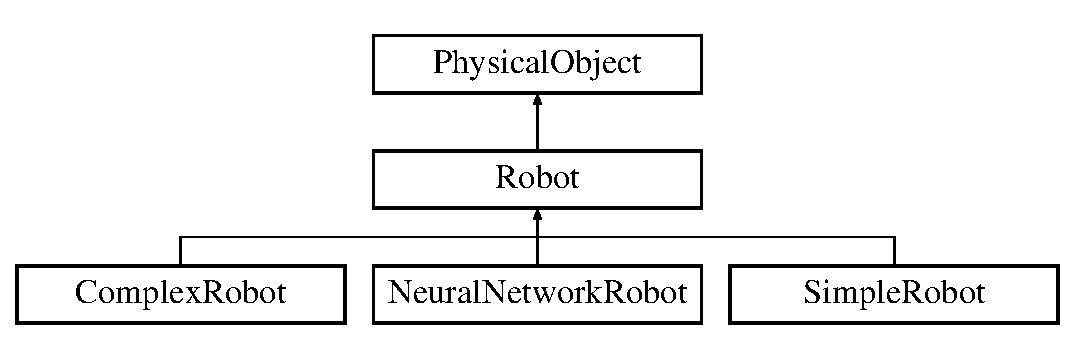
\includegraphics[height=3.000000cm]{classRobot}
\end{center}
\end{figure}
\subsection*{Public Member Functions}
\begin{DoxyCompactItemize}
\item 
\hyperlink{classRobot_a2ddd4ae79de00f20b5ceb2df49f7d05e}{Robot} (\hyperlink{Robot_8h_a78d284d08fd22d809fd436256f2cbc39}{Robot\-Type} \hyperlink{classRobot_a49eb06af6d6981c941a24edc54210316}{robot\-Type}, int radius, \hyperlink{structColor}{Color} color, \hyperlink{structColor}{Color} line\-Color, int target\-Id=-\/1)
\item 
\hyperlink{classRobot_a3fa5c6664ffed53633e6e90fd398c287}{Robot} (\hyperlink{Robot_8h_a78d284d08fd22d809fd436256f2cbc39}{Robot\-Type} \hyperlink{classRobot_a49eb06af6d6981c941a24edc54210316}{robot\-Type}, int radius, \hyperlink{structLocation}{Location} loc, \hyperlink{structColor}{Color} color, \hyperlink{structColor}{Color} line\-Color, int target\-Id=-\/1)
\item 
\hyperlink{classRobot_a924320124b09c2f2ac1621aa210d5f38}{$\sim$\-Robot} ()
\item 
int \hyperlink{classRobot_a23f5bb01abf88e4c0edd370949080a4c}{get\-Target} () const 
\item 
void \hyperlink{classRobot_aa1b41b16fe5609310c4b7d23a4553970}{set\-Target} (int id)
\item 
bool \hyperlink{classRobot_a94d8b5083b9426e3769a5f84f310093e}{handle\-Collision} (int other\-Id, bool was\-Hit)
\item 
void \hyperlink{classRobot_adc34eec22821c2dce23904a5ea75cf13}{update} ()
\item 
void \hyperlink{classRobot_a6f8e6aaedcb7c130d37b5e653faea070}{update\-Members} ()
\item 
void \hyperlink{classRobot_a079c44b63ede22b1b6be4297934886da}{display} ()
\item 
void \hyperlink{classRobot_a9a44e2faef3d3927473ac0bacad8b670}{set\-Line\-Color} (\hyperlink{structColor}{Color} line\-Color)
\item 
\hyperlink{structColor}{Color} \hyperlink{classRobot_adf3e43c63f0173fe05cc35ef8d607aca}{get\-Line\-Color} ()
\end{DoxyCompactItemize}
\subsection*{Public Attributes}
\begin{DoxyCompactItemize}
\item 
const \hyperlink{Robot_8h_a78d284d08fd22d809fd436256f2cbc39}{Robot\-Type} \hyperlink{classRobot_a49eb06af6d6981c941a24edc54210316}{robot\-Type}
\end{DoxyCompactItemize}
\subsection*{Protected Member Functions}
\begin{DoxyCompactItemize}
\item 
virtual float \hyperlink{classRobot_a9c96f301ae826e7c535f6b705e44bcd6}{get\-Left\-Speed} (float left\-Light\-Sensor\-Val, float right\-Light\-Sensor\-Val, float left\-Robot\-Sensor\-Val, float right\-Robot\-Sensor\-Val, float left\-Obstacle\-Sensor\-Val, float right\-Obstacle\-Sensor\-Val, float left\-Target\-Sensor\-Val, float right\-Target\-Sensor\-Val)=0
\item 
virtual float \hyperlink{classRobot_a3289251979084c50b18a6006547d3f95}{get\-Right\-Speed} (float left\-Light\-Sensor\-Val, float right\-Light\-Sensor\-Val, float left\-Robot\-Sensor\-Val, float right\-Robot\-Sensor\-Val, float left\-Obstacle\-Sensor\-Val, float right\-Obstacle\-Sensor\-Val, float left\-Target\-Sensor\-Val, float right\-Target\-Sensor\-Val)=0
\end{DoxyCompactItemize}
\subsection*{Additional Inherited Members}


\subsection{Detailed Description}
\hyperlink{classRobot}{Robot} that moves around the window and bumps into obstacles. 

\subsection{Constructor \& Destructor Documentation}
\hypertarget{classRobot_a2ddd4ae79de00f20b5ceb2df49f7d05e}{\index{Robot@{Robot}!Robot@{Robot}}
\index{Robot@{Robot}!Robot@{Robot}}
\subsubsection[{Robot}]{\setlength{\rightskip}{0pt plus 5cm}Robot\-::\-Robot (
\begin{DoxyParamCaption}
\item[{{\bf Robot\-Type}}]{robot\-Type, }
\item[{int}]{radius, }
\item[{{\bf Color}}]{color, }
\item[{{\bf Color}}]{line\-Color, }
\item[{int}]{target\-Id = {\ttfamily -\/1}}
\end{DoxyParamCaption}
)}}\label{classRobot_a2ddd4ae79de00f20b5ceb2df49f7d05e}

\begin{DoxyParams}{Parameters}
{\em robot\-Type} & the robot type \\
\hline
{\em radius} & the radius in pixels \\
\hline
{\em color} & color of the robot itself, a struct of float value 0 to 1 representing a hexedecimal color \\
\hline
{\em line\-Color} & color of the line, a struct of float value 0 to 1 representing a hexedecimal color \\
\hline
\end{DoxyParams}
\begin{DoxyParagraph}{Initialization}
\hyperlink{classRobot}{Robot} is initialized with the following values\-: 
\end{DoxyParagraph}


Orientation\-: 0 

Speed\-: 0 

Position\-: (loc.\-x, loc.\-y)   \hypertarget{classRobot_a3fa5c6664ffed53633e6e90fd398c287}{\index{Robot@{Robot}!Robot@{Robot}}
\index{Robot@{Robot}!Robot@{Robot}}
\subsubsection[{Robot}]{\setlength{\rightskip}{0pt plus 5cm}Robot\-::\-Robot (
\begin{DoxyParamCaption}
\item[{{\bf Robot\-Type}}]{robot\-Type, }
\item[{int}]{radius, }
\item[{{\bf Location}}]{loc, }
\item[{{\bf Color}}]{color, }
\item[{{\bf Color}}]{line\-Color, }
\item[{int}]{target\-Id = {\ttfamily -\/1}}
\end{DoxyParamCaption}
)}}\label{classRobot_a3fa5c6664ffed53633e6e90fd398c287}

\begin{DoxyParams}{Parameters}
{\em robot\-Type} & the robot type \\
\hline
{\em radius} & the radius in pixels \\
\hline
{\em color} & a struct of float value 0 to 1 representing a hexedecimal color \\
\hline
{\em linecolor} & color of the line, a struct of float value 0 to 1 representing a hexedecimal color \\
\hline
{\em loc} & start \hyperlink{structLocation}{Location} of the robot \\
\hline
\end{DoxyParams}
\begin{DoxyParagraph}{Initialization}
\hyperlink{classRobot}{Robot} is initialized with the following values\-: 
\end{DoxyParagraph}


Orientation\-: random 

Speed\-: 0 

Position\-: (loc.\-x, loc.\-y)   \hypertarget{classRobot_a924320124b09c2f2ac1621aa210d5f38}{\index{Robot@{Robot}!$\sim$\-Robot@{$\sim$\-Robot}}
\index{$\sim$\-Robot@{$\sim$\-Robot}!Robot@{Robot}}
\subsubsection[{$\sim$\-Robot}]{\setlength{\rightskip}{0pt plus 5cm}Robot\-::$\sim$\-Robot (
\begin{DoxyParamCaption}
{}
\end{DoxyParamCaption}
)}}\label{classRobot_a924320124b09c2f2ac1621aa210d5f38}
This is the class destructor. 

\subsection{Member Function Documentation}
\hypertarget{classRobot_a079c44b63ede22b1b6be4297934886da}{\index{Robot@{Robot}!display@{display}}
\index{display@{display}!Robot@{Robot}}
\subsubsection[{display}]{\setlength{\rightskip}{0pt plus 5cm}void Robot\-::display (
\begin{DoxyParamCaption}
{}
\end{DoxyParamCaption}
)\hspace{0.3cm}{\ttfamily [virtual]}}}\label{classRobot_a079c44b63ede22b1b6be4297934886da}
\begin{DoxyAuthor}{Author}
Lucas Kramer This function displays the \hyperlink{classRobot}{Robot} in the graphics 
\end{DoxyAuthor}


Reimplemented from \hyperlink{classPhysicalObject_a6a0326df3efc0a1ea23892e3fcd4b11e}{Physical\-Object}.

\hypertarget{classRobot_a9c96f301ae826e7c535f6b705e44bcd6}{\index{Robot@{Robot}!get\-Left\-Speed@{get\-Left\-Speed}}
\index{get\-Left\-Speed@{get\-Left\-Speed}!Robot@{Robot}}
\subsubsection[{get\-Left\-Speed}]{\setlength{\rightskip}{0pt plus 5cm}virtual float Robot\-::get\-Left\-Speed (
\begin{DoxyParamCaption}
\item[{float}]{left\-Light\-Sensor\-Val, }
\item[{float}]{right\-Light\-Sensor\-Val, }
\item[{float}]{left\-Robot\-Sensor\-Val, }
\item[{float}]{right\-Robot\-Sensor\-Val, }
\item[{float}]{left\-Obstacle\-Sensor\-Val, }
\item[{float}]{right\-Obstacle\-Sensor\-Val, }
\item[{float}]{left\-Target\-Sensor\-Val, }
\item[{float}]{right\-Target\-Sensor\-Val}
\end{DoxyParamCaption}
)\hspace{0.3cm}{\ttfamily [protected]}, {\ttfamily [pure virtual]}}}\label{classRobot_a9c96f301ae826e7c535f6b705e44bcd6}


Implemented in \hyperlink{classComplexRobot_aa50c7f5ed4f288987fe2557b41a9bf32}{Complex\-Robot}, \hyperlink{classNeuralNetworkRobot_a91c4210b62175e9ffb1ed3362df318af}{Neural\-Network\-Robot}, and \hyperlink{classSimpleRobot_a3dd2f39fc84a1d9fa4384c69255b3e79}{Simple\-Robot}.

\hypertarget{classRobot_adf3e43c63f0173fe05cc35ef8d607aca}{\index{Robot@{Robot}!get\-Line\-Color@{get\-Line\-Color}}
\index{get\-Line\-Color@{get\-Line\-Color}!Robot@{Robot}}
\subsubsection[{get\-Line\-Color}]{\setlength{\rightskip}{0pt plus 5cm}{\bf Color} Robot\-::get\-Line\-Color (
\begin{DoxyParamCaption}
{}
\end{DoxyParamCaption}
)}}\label{classRobot_adf3e43c63f0173fe05cc35ef8d607aca}
\hypertarget{classRobot_a3289251979084c50b18a6006547d3f95}{\index{Robot@{Robot}!get\-Right\-Speed@{get\-Right\-Speed}}
\index{get\-Right\-Speed@{get\-Right\-Speed}!Robot@{Robot}}
\subsubsection[{get\-Right\-Speed}]{\setlength{\rightskip}{0pt plus 5cm}virtual float Robot\-::get\-Right\-Speed (
\begin{DoxyParamCaption}
\item[{float}]{left\-Light\-Sensor\-Val, }
\item[{float}]{right\-Light\-Sensor\-Val, }
\item[{float}]{left\-Robot\-Sensor\-Val, }
\item[{float}]{right\-Robot\-Sensor\-Val, }
\item[{float}]{left\-Obstacle\-Sensor\-Val, }
\item[{float}]{right\-Obstacle\-Sensor\-Val, }
\item[{float}]{left\-Target\-Sensor\-Val, }
\item[{float}]{right\-Target\-Sensor\-Val}
\end{DoxyParamCaption}
)\hspace{0.3cm}{\ttfamily [protected]}, {\ttfamily [pure virtual]}}}\label{classRobot_a3289251979084c50b18a6006547d3f95}


Implemented in \hyperlink{classComplexRobot_ac038c2dbcc242d68a3ef9e533673bdf6}{Complex\-Robot}, \hyperlink{classNeuralNetworkRobot_a7b3389e89eb3485ad9e074494624e204}{Neural\-Network\-Robot}, and \hyperlink{classSimpleRobot_ae94b1dd9d31f2cbeb21fcbd5413a8a3a}{Simple\-Robot}.

\hypertarget{classRobot_a23f5bb01abf88e4c0edd370949080a4c}{\index{Robot@{Robot}!get\-Target@{get\-Target}}
\index{get\-Target@{get\-Target}!Robot@{Robot}}
\subsubsection[{get\-Target}]{\setlength{\rightskip}{0pt plus 5cm}int Robot\-::get\-Target (
\begin{DoxyParamCaption}
{}
\end{DoxyParamCaption}
) const}}\label{classRobot_a23f5bb01abf88e4c0edd370949080a4c}
\begin{DoxyAuthor}{Author}
Lucas Kramer This function gets the id of the target for the robot to seek. 
\end{DoxyAuthor}

\begin{DoxyParams}{Parameters}
{\em id} & the id of the target \\
\hline
\end{DoxyParams}
\hypertarget{classRobot_a94d8b5083b9426e3769a5f84f310093e}{\index{Robot@{Robot}!handle\-Collision@{handle\-Collision}}
\index{handle\-Collision@{handle\-Collision}!Robot@{Robot}}
\subsubsection[{handle\-Collision}]{\setlength{\rightskip}{0pt plus 5cm}bool Robot\-::handle\-Collision (
\begin{DoxyParamCaption}
\item[{int}]{other\-Id, }
\item[{bool}]{was\-Hit}
\end{DoxyParamCaption}
)\hspace{0.3cm}{\ttfamily [virtual]}}}\label{classRobot_a94d8b5083b9426e3769a5f84f310093e}
\begin{DoxyAuthor}{Author}
Lucas Kramer This function gives \hyperlink{classRobot}{Robot} an appropriate reaction when a collision occurs 
\end{DoxyAuthor}

\begin{DoxyParams}{Parameters}
{\em other\-Id} & id of the object that it collides with \\
\hline
{\em was\-Hit} & tells if the object was hit previously \\
\hline
\end{DoxyParams}


Implements \hyperlink{classPhysicalObject_a400ba3545479ebbf8b1b4a046906e562}{Physical\-Object}.

\hypertarget{classRobot_a9a44e2faef3d3927473ac0bacad8b670}{\index{Robot@{Robot}!set\-Line\-Color@{set\-Line\-Color}}
\index{set\-Line\-Color@{set\-Line\-Color}!Robot@{Robot}}
\subsubsection[{set\-Line\-Color}]{\setlength{\rightskip}{0pt plus 5cm}void Robot\-::set\-Line\-Color (
\begin{DoxyParamCaption}
\item[{{\bf Color}}]{line\-Color}
\end{DoxyParamCaption}
)}}\label{classRobot_a9a44e2faef3d3927473ac0bacad8b670}
\begin{DoxyAuthor}{Author}
Lucas Kramer This function sets a new color for the robot's direction line. 
\end{DoxyAuthor}

\begin{DoxyParams}{Parameters}
{\em line\-Color} & color of the line, a struct of float value 0 to 1 representing a hexedecimal color \\
\hline
\end{DoxyParams}
\hypertarget{classRobot_aa1b41b16fe5609310c4b7d23a4553970}{\index{Robot@{Robot}!set\-Target@{set\-Target}}
\index{set\-Target@{set\-Target}!Robot@{Robot}}
\subsubsection[{set\-Target}]{\setlength{\rightskip}{0pt plus 5cm}void Robot\-::set\-Target (
\begin{DoxyParamCaption}
\item[{int}]{id}
\end{DoxyParamCaption}
)}}\label{classRobot_aa1b41b16fe5609310c4b7d23a4553970}
\begin{DoxyAuthor}{Author}
Lucas Kramer This function sets the id of the target for the robot to seek. 
\end{DoxyAuthor}
\begin{DoxyReturn}{Returns}
the target id 
\end{DoxyReturn}
\hypertarget{classRobot_adc34eec22821c2dce23904a5ea75cf13}{\index{Robot@{Robot}!update@{update}}
\index{update@{update}!Robot@{Robot}}
\subsubsection[{update}]{\setlength{\rightskip}{0pt plus 5cm}void Robot\-::update (
\begin{DoxyParamCaption}
{}
\end{DoxyParamCaption}
)\hspace{0.3cm}{\ttfamily [virtual]}}}\label{classRobot_adc34eec22821c2dce23904a5ea75cf13}
\begin{DoxyAuthor}{Author}
Lucas Kramer This function updates the \hyperlink{classRobot}{Robot}'s wheel speeds from the sensors 
\end{DoxyAuthor}


Reimplemented from \hyperlink{classPhysicalObject_a3005ac0afce838049101db17525f6004}{Physical\-Object}.

\hypertarget{classRobot_a6f8e6aaedcb7c130d37b5e653faea070}{\index{Robot@{Robot}!update\-Members@{update\-Members}}
\index{update\-Members@{update\-Members}!Robot@{Robot}}
\subsubsection[{update\-Members}]{\setlength{\rightskip}{0pt plus 5cm}void Robot\-::update\-Members (
\begin{DoxyParamCaption}
{}
\end{DoxyParamCaption}
)\hspace{0.3cm}{\ttfamily [virtual]}}}\label{classRobot_a6f8e6aaedcb7c130d37b5e653faea070}
\begin{DoxyAuthor}{Author}
Lucas Kramer This function updates the position of the robot's sub-\/objects 
\end{DoxyAuthor}


Reimplemented from \hyperlink{classPhysicalObject_a4fc8c0c62b8e12a63ebdf13136d577ac}{Physical\-Object}.



\subsection{Member Data Documentation}
\hypertarget{classRobot_a49eb06af6d6981c941a24edc54210316}{\index{Robot@{Robot}!robot\-Type@{robot\-Type}}
\index{robot\-Type@{robot\-Type}!Robot@{Robot}}
\subsubsection[{robot\-Type}]{\setlength{\rightskip}{0pt plus 5cm}const {\bf Robot\-Type} Robot\-::robot\-Type}}\label{classRobot_a49eb06af6d6981c941a24edc54210316}


The documentation for this class was generated from the following files\-:\begin{DoxyCompactItemize}
\item 
\hyperlink{Robot_8h}{Robot.\-h}\item 
\hyperlink{Robot_8cpp}{Robot.\-cpp}\end{DoxyCompactItemize}

\hypertarget{classSensor}{\section{Sensor Class Reference}
\label{classSensor}\index{Sensor@{Sensor}}
}


{\ttfamily \#include $<$Sensor.\-h$>$}

\subsection*{Public Member Functions}
\begin{DoxyCompactItemize}
\item 
\hyperlink{classSensor_a37f7683054a1cd9ea12834b702d8886d}{Sensor} (\hyperlink{structLocation}{Location} loc, int orientation, \hyperlink{PhysicalObject_8h_a842c5e2e69277690b064bf363c017980}{Object\-Type} type\-Detected)
\item 
\hyperlink{classSensor_a8db2f6b1569016548b226725e4eb3301}{Sensor} (\hyperlink{structLocation}{Location} loc, int orientation, int view\-Angle, \hyperlink{PhysicalObject_8h_a842c5e2e69277690b064bf363c017980}{Object\-Type} type\-Detected)
\item 
void \hyperlink{classSensor_addabbd59236833da1adfe341e4c18f80}{set\-Position} (float x, float y)
\item 
void \hyperlink{classSensor_ab177881093c0f4dc22f5951f27638c86}{set\-Position} (\hyperlink{structLocation}{Location} loc)
\item 
\hyperlink{structLocation}{Location} \hyperlink{classSensor_a021d0c08cc8cdf5d7eae9b58af02589f}{get\-Position} ()
\item 
float \hyperlink{classSensor_a32aadaf1e0c393eea51ee54df853cd7b}{get\-X\-Position} ()
\item 
float \hyperlink{classSensor_a87d42b5670accfc0dff1abc438875a73}{get\-Y\-Position} ()
\item 
void \hyperlink{classSensor_ae496cb993bf7c3b4876527a36ae95272}{set\-Orientation} (int orientation)
\item 
int \hyperlink{classSensor_a178e33bafb97b61319f17325223cf7de}{get\-Orientation} ()
\item 
void \hyperlink{classSensor_ad2138006b3d6a7779b17fd84e5a6f081}{set\-View\-Angle} (int degrees)
\item 
int \hyperlink{classSensor_ab5bc3039acc0d11c9cefb08515452aff}{get\-View\-Angle} ()
\item 
void \hyperlink{classSensor_a10ab10a83beb503b30a3a950149a2da9}{set\-Type\-Detected} (\hyperlink{PhysicalObject_8h_a842c5e2e69277690b064bf363c017980}{Object\-Type} type)
\item 
\hyperlink{PhysicalObject_8h_a842c5e2e69277690b064bf363c017980}{Object\-Type} \hyperlink{classSensor_a8c43057ed1d49be620595262ae720281}{get\-Type\-Detected} ()
\item 
void \hyperlink{classSensor_a9a2b1a48810e63b3d0621e8cea1ef81f}{update\-Position} (\hyperlink{structLocation}{Location} robot\-Loc, int robot\-Angle)
\item 
void \hyperlink{classSensor_ac77b1ae6ae7b06dcc60127c7cef88336}{display} ()
\item 
float \hyperlink{classSensor_ac0aad8c71f6156d2c8c626b304e67595}{sense} ()
\end{DoxyCompactItemize}


\subsection{Constructor \& Destructor Documentation}
\hypertarget{classSensor_a37f7683054a1cd9ea12834b702d8886d}{\index{Sensor@{Sensor}!Sensor@{Sensor}}
\index{Sensor@{Sensor}!Sensor@{Sensor}}
\subsubsection[{Sensor}]{\setlength{\rightskip}{0pt plus 5cm}Sensor\-::\-Sensor (
\begin{DoxyParamCaption}
\item[{{\bf Location}}]{loc, }
\item[{int}]{orientation, }
\item[{{\bf Object\-Type}}]{type\-Detected}
\end{DoxyParamCaption}
)}}\label{classSensor_a37f7683054a1cd9ea12834b702d8886d}
\hyperlink{classSensor}{Sensor} constructor with default angle 
\begin{DoxyParams}{Parameters}
{\em loc} & \hyperlink{structLocation}{Location} of the sensor in x and y \\
\hline
{\em orientation} & orientation of the sensor \\
\hline
{\em type\-Detected} & type that sensor will detect \\
\hline
\end{DoxyParams}
\hypertarget{classSensor_a8db2f6b1569016548b226725e4eb3301}{\index{Sensor@{Sensor}!Sensor@{Sensor}}
\index{Sensor@{Sensor}!Sensor@{Sensor}}
\subsubsection[{Sensor}]{\setlength{\rightskip}{0pt plus 5cm}Sensor\-::\-Sensor (
\begin{DoxyParamCaption}
\item[{{\bf Location}}]{loc, }
\item[{int}]{orientation, }
\item[{int}]{view\-Angle, }
\item[{{\bf Object\-Type}}]{type\-Detected}
\end{DoxyParamCaption}
)}}\label{classSensor_a8db2f6b1569016548b226725e4eb3301}
\hyperlink{classSensor}{Sensor} constructor 
\begin{DoxyParams}{Parameters}
{\em loc} & \hyperlink{structLocation}{Location} of the sensor in x and y \\
\hline
{\em orientation} & orientation of the sensor \\
\hline
{\em view\-Angle} & view angle of the sensor in degrees \\
\hline
{\em type\-Detected} & type that sensor will detect \\
\hline
\end{DoxyParams}


\subsection{Member Function Documentation}
\hypertarget{classSensor_ac77b1ae6ae7b06dcc60127c7cef88336}{\index{Sensor@{Sensor}!display@{display}}
\index{display@{display}!Sensor@{Sensor}}
\subsubsection[{display}]{\setlength{\rightskip}{0pt plus 5cm}void Sensor\-::display (
\begin{DoxyParamCaption}
{}
\end{DoxyParamCaption}
)}}\label{classSensor_ac77b1ae6ae7b06dcc60127c7cef88336}
Displays the sensor \begin{DoxyAuthor}{Author}
Carl 
\end{DoxyAuthor}
\hypertarget{classSensor_a178e33bafb97b61319f17325223cf7de}{\index{Sensor@{Sensor}!get\-Orientation@{get\-Orientation}}
\index{get\-Orientation@{get\-Orientation}!Sensor@{Sensor}}
\subsubsection[{get\-Orientation}]{\setlength{\rightskip}{0pt plus 5cm}int Sensor\-::get\-Orientation (
\begin{DoxyParamCaption}
{}
\end{DoxyParamCaption}
)}}\label{classSensor_a178e33bafb97b61319f17325223cf7de}
Returns the orientation of the sensor \begin{DoxyReturn}{Returns}
orientation in degrees 
\end{DoxyReturn}
\hypertarget{classSensor_a021d0c08cc8cdf5d7eae9b58af02589f}{\index{Sensor@{Sensor}!get\-Position@{get\-Position}}
\index{get\-Position@{get\-Position}!Sensor@{Sensor}}
\subsubsection[{get\-Position}]{\setlength{\rightskip}{0pt plus 5cm}{\bf Location} Sensor\-::get\-Position (
\begin{DoxyParamCaption}
{}
\end{DoxyParamCaption}
)}}\label{classSensor_a021d0c08cc8cdf5d7eae9b58af02589f}
Returns a \hyperlink{structLocation}{Location} struct of x and y position in pixels of the sensor \begin{DoxyReturn}{Returns}
A \hyperlink{structLocation}{Location} struct of x and y position 
\end{DoxyReturn}
\hypertarget{classSensor_a8c43057ed1d49be620595262ae720281}{\index{Sensor@{Sensor}!get\-Type\-Detected@{get\-Type\-Detected}}
\index{get\-Type\-Detected@{get\-Type\-Detected}!Sensor@{Sensor}}
\subsubsection[{get\-Type\-Detected}]{\setlength{\rightskip}{0pt plus 5cm}{\bf Object\-Type} Sensor\-::get\-Type\-Detected (
\begin{DoxyParamCaption}
{}
\end{DoxyParamCaption}
)}}\label{classSensor_a8c43057ed1d49be620595262ae720281}
Returns the type that sensor detects \begin{DoxyAuthor}{Author}
Himawan 
\end{DoxyAuthor}
\begin{DoxyReturn}{Returns}
type the sensor detects 
\end{DoxyReturn}
\hypertarget{classSensor_ab5bc3039acc0d11c9cefb08515452aff}{\index{Sensor@{Sensor}!get\-View\-Angle@{get\-View\-Angle}}
\index{get\-View\-Angle@{get\-View\-Angle}!Sensor@{Sensor}}
\subsubsection[{get\-View\-Angle}]{\setlength{\rightskip}{0pt plus 5cm}int Sensor\-::get\-View\-Angle (
\begin{DoxyParamCaption}
{}
\end{DoxyParamCaption}
)}}\label{classSensor_ab5bc3039acc0d11c9cefb08515452aff}
Returns the view angle of the sensor \begin{DoxyReturn}{Returns}
view angle in degrees 
\end{DoxyReturn}
\hypertarget{classSensor_a32aadaf1e0c393eea51ee54df853cd7b}{\index{Sensor@{Sensor}!get\-X\-Position@{get\-X\-Position}}
\index{get\-X\-Position@{get\-X\-Position}!Sensor@{Sensor}}
\subsubsection[{get\-X\-Position}]{\setlength{\rightskip}{0pt plus 5cm}float Sensor\-::get\-X\-Position (
\begin{DoxyParamCaption}
{}
\end{DoxyParamCaption}
)}}\label{classSensor_a32aadaf1e0c393eea51ee54df853cd7b}
Returns the x position in pixels of the sensor \begin{DoxyReturn}{Returns}
x position 
\end{DoxyReturn}
\hypertarget{classSensor_a87d42b5670accfc0dff1abc438875a73}{\index{Sensor@{Sensor}!get\-Y\-Position@{get\-Y\-Position}}
\index{get\-Y\-Position@{get\-Y\-Position}!Sensor@{Sensor}}
\subsubsection[{get\-Y\-Position}]{\setlength{\rightskip}{0pt plus 5cm}float Sensor\-::get\-Y\-Position (
\begin{DoxyParamCaption}
{}
\end{DoxyParamCaption}
)}}\label{classSensor_a87d42b5670accfc0dff1abc438875a73}
Returns the y position in pixels of the sensor \begin{DoxyReturn}{Returns}
y position 
\end{DoxyReturn}
\hypertarget{classSensor_ac0aad8c71f6156d2c8c626b304e67595}{\index{Sensor@{Sensor}!sense@{sense}}
\index{sense@{sense}!Sensor@{Sensor}}
\subsubsection[{sense}]{\setlength{\rightskip}{0pt plus 5cm}float Sensor\-::sense (
\begin{DoxyParamCaption}
{}
\end{DoxyParamCaption}
)}}\label{classSensor_ac0aad8c71f6156d2c8c626b304e67595}
Returns some strength by sensing the environment \begin{DoxyAuthor}{Author}
Carl \& Himawan 
\end{DoxyAuthor}
\begin{DoxyReturn}{Returns}
the strength of sensor reading of \mbox{[}0..1\mbox{]} 
\end{DoxyReturn}
\hypertarget{classSensor_ae496cb993bf7c3b4876527a36ae95272}{\index{Sensor@{Sensor}!set\-Orientation@{set\-Orientation}}
\index{set\-Orientation@{set\-Orientation}!Sensor@{Sensor}}
\subsubsection[{set\-Orientation}]{\setlength{\rightskip}{0pt plus 5cm}void Sensor\-::set\-Orientation (
\begin{DoxyParamCaption}
\item[{int}]{orientation}
\end{DoxyParamCaption}
)}}\label{classSensor_ae496cb993bf7c3b4876527a36ae95272}
Sets the orientation for the sensor 
\begin{DoxyParams}{Parameters}
{\em orientation} & The orientation of the object in degrees \\
\hline
\end{DoxyParams}
\hypertarget{classSensor_addabbd59236833da1adfe341e4c18f80}{\index{Sensor@{Sensor}!set\-Position@{set\-Position}}
\index{set\-Position@{set\-Position}!Sensor@{Sensor}}
\subsubsection[{set\-Position}]{\setlength{\rightskip}{0pt plus 5cm}void Sensor\-::set\-Position (
\begin{DoxyParamCaption}
\item[{float}]{x, }
\item[{float}]{y}
\end{DoxyParamCaption}
)}}\label{classSensor_addabbd59236833da1adfe341e4c18f80}
Sets the position for the sensor 
\begin{DoxyParams}{Parameters}
{\em x} & x position in pixels \\
\hline
{\em y} & y position in pixels \\
\hline
\end{DoxyParams}
\hypertarget{classSensor_ab177881093c0f4dc22f5951f27638c86}{\index{Sensor@{Sensor}!set\-Position@{set\-Position}}
\index{set\-Position@{set\-Position}!Sensor@{Sensor}}
\subsubsection[{set\-Position}]{\setlength{\rightskip}{0pt plus 5cm}void Sensor\-::set\-Position (
\begin{DoxyParamCaption}
\item[{{\bf Location}}]{loc}
\end{DoxyParamCaption}
)}}\label{classSensor_ab177881093c0f4dc22f5951f27638c86}
Sets the position for the sensor 
\begin{DoxyParams}{Parameters}
{\em loc} & A struct of the x and y \hyperlink{structLocation}{Location} in pixels \\
\hline
\end{DoxyParams}
\hypertarget{classSensor_a10ab10a83beb503b30a3a950149a2da9}{\index{Sensor@{Sensor}!set\-Type\-Detected@{set\-Type\-Detected}}
\index{set\-Type\-Detected@{set\-Type\-Detected}!Sensor@{Sensor}}
\subsubsection[{set\-Type\-Detected}]{\setlength{\rightskip}{0pt plus 5cm}void Sensor\-::set\-Type\-Detected (
\begin{DoxyParamCaption}
\item[{{\bf Object\-Type}}]{type}
\end{DoxyParamCaption}
)}}\label{classSensor_a10ab10a83beb503b30a3a950149a2da9}
Sets the object type that the sensor detects \begin{DoxyAuthor}{Author}
Himawan 
\end{DoxyAuthor}

\begin{DoxyParams}{Parameters}
{\em type} & object type to detect \\
\hline
\end{DoxyParams}
\hypertarget{classSensor_ad2138006b3d6a7779b17fd84e5a6f081}{\index{Sensor@{Sensor}!set\-View\-Angle@{set\-View\-Angle}}
\index{set\-View\-Angle@{set\-View\-Angle}!Sensor@{Sensor}}
\subsubsection[{set\-View\-Angle}]{\setlength{\rightskip}{0pt plus 5cm}void Sensor\-::set\-View\-Angle (
\begin{DoxyParamCaption}
\item[{int}]{degrees}
\end{DoxyParamCaption}
)}}\label{classSensor_ad2138006b3d6a7779b17fd84e5a6f081}
Sets the view angle of the sensor 
\begin{DoxyParams}{Parameters}
{\em degrees} & The view angle of the sensor in degrees \\
\hline
\end{DoxyParams}
\hypertarget{classSensor_a9a2b1a48810e63b3d0621e8cea1ef81f}{\index{Sensor@{Sensor}!update\-Position@{update\-Position}}
\index{update\-Position@{update\-Position}!Sensor@{Sensor}}
\subsubsection[{update\-Position}]{\setlength{\rightskip}{0pt plus 5cm}void Sensor\-::update\-Position (
\begin{DoxyParamCaption}
\item[{{\bf Location}}]{robot\-Loc, }
\item[{int}]{robot\-Angle}
\end{DoxyParamCaption}
)}}\label{classSensor_a9a2b1a48810e63b3d0621e8cea1ef81f}
Called to update the position of the sensor match the updated position of the robot \begin{DoxyAuthor}{Author}
Carl 
\end{DoxyAuthor}


The documentation for this class was generated from the following files\-:\begin{DoxyCompactItemize}
\item 
\hyperlink{Sensor_8h}{Sensor.\-h}\item 
\hyperlink{Sensor_8cpp}{Sensor.\-cpp}\end{DoxyCompactItemize}

\hypertarget{classSimpleRobot}{\section{Simple\-Robot Class Reference}
\label{classSimpleRobot}\index{Simple\-Robot@{Simple\-Robot}}
}


A simple robot with uncrossed feedback.  




{\ttfamily \#include $<$Simple\-Robot.\-h$>$}

Inheritance diagram for Simple\-Robot\-:\begin{figure}[H]
\begin{center}
\leavevmode
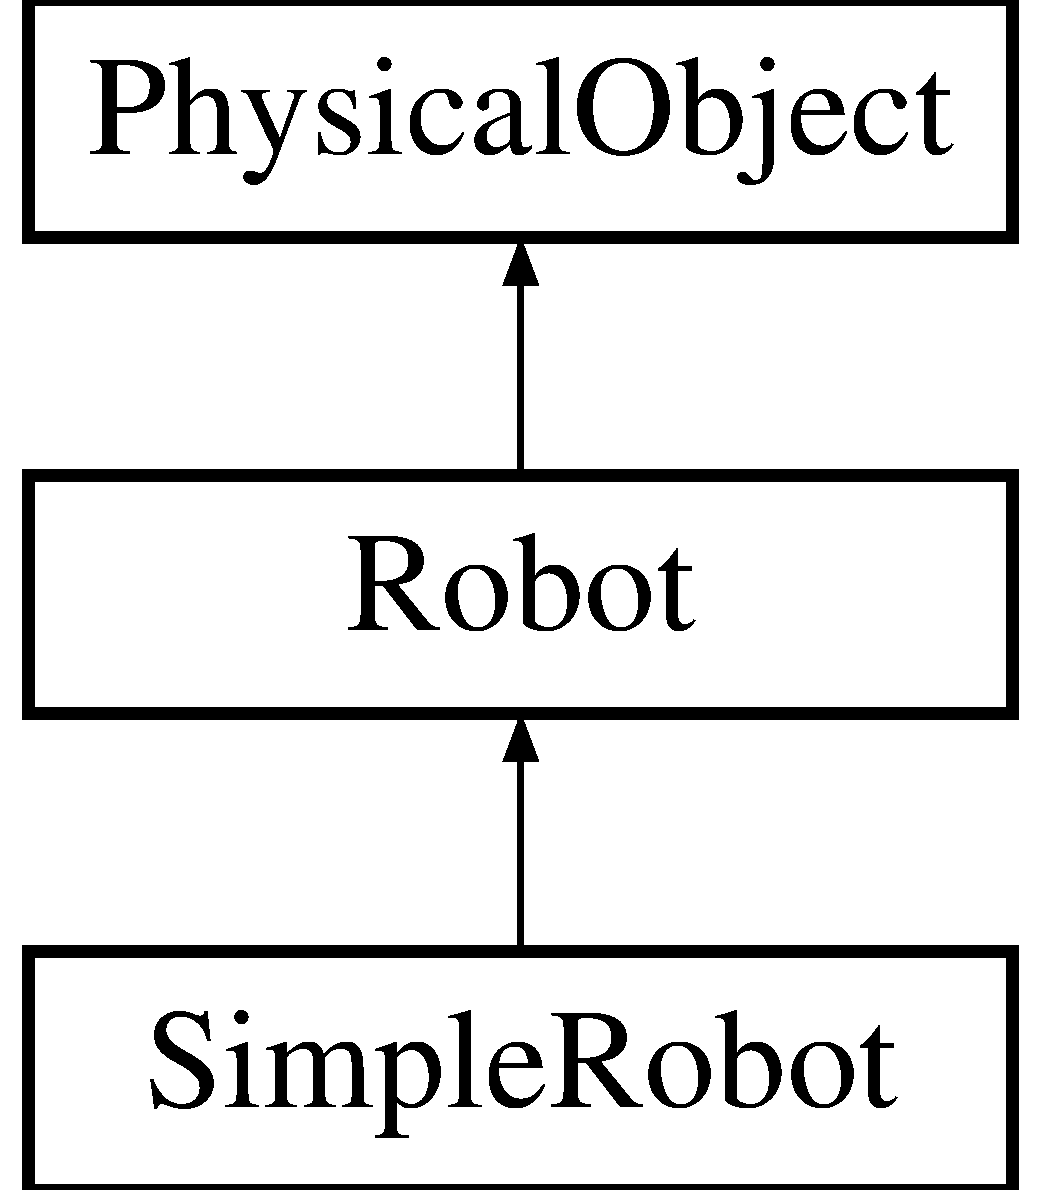
\includegraphics[height=3.000000cm]{classSimpleRobot}
\end{center}
\end{figure}
\subsection*{Public Member Functions}
\begin{DoxyCompactItemize}
\item 
\hyperlink{classSimpleRobot_a9ec65d80f5c030931fc07ab3ee5febb1}{Simple\-Robot} (int radius, \hyperlink{structColor}{Color} color, \hyperlink{structColor}{Color} line\-Color, int target\-Id=-\/1)
\item 
\hyperlink{classSimpleRobot_acad9f0762a53f5c294aff27ca2e433ce}{Simple\-Robot} (int radius, \hyperlink{structLocation}{Location} loc, \hyperlink{structColor}{Color} color, \hyperlink{structColor}{Color} line\-Color, int target\-Id=-\/1)
\item 
\hyperlink{classSimpleRobot_a3ef1551c84858e2b2c558d15380ced06}{$\sim$\-Simple\-Robot} ()
\item 
float \hyperlink{classSimpleRobot_a3dd2f39fc84a1d9fa4384c69255b3e79}{get\-Left\-Speed} (float left\-Light\-Sensor\-Val, float right\-Light\-Sensor\-Val, float left\-Robot\-Sensor\-Val, float right\-Robot\-Sensor\-Val, float left\-Obstacle\-Sensor\-Val, float right\-Obstacle\-Sensor\-Val, float left\-Target\-Sensor\-Val, float right\-Target\-Sensor\-Val)
\item 
float \hyperlink{classSimpleRobot_ae94b1dd9d31f2cbeb21fcbd5413a8a3a}{get\-Right\-Speed} (float left\-Light\-Sensor\-Val, float right\-Light\-Sensor\-Val, float left\-Robot\-Sensor\-Val, float right\-Robot\-Sensor\-Val, float left\-Obstacle\-Sensor\-Val, float right\-Obstacle\-Sensor\-Val, float left\-Target\-Sensor\-Val, float right\-Target\-Sensor\-Val)
\end{DoxyCompactItemize}
\subsection*{Additional Inherited Members}


\subsection{Detailed Description}
A simple robot with uncrossed feedback. 

\subsection{Constructor \& Destructor Documentation}
\hypertarget{classSimpleRobot_a9ec65d80f5c030931fc07ab3ee5febb1}{\index{Simple\-Robot@{Simple\-Robot}!Simple\-Robot@{Simple\-Robot}}
\index{Simple\-Robot@{Simple\-Robot}!SimpleRobot@{Simple\-Robot}}
\subsubsection[{Simple\-Robot}]{\setlength{\rightskip}{0pt plus 5cm}Simple\-Robot\-::\-Simple\-Robot (
\begin{DoxyParamCaption}
\item[{int}]{radius, }
\item[{{\bf Color}}]{color, }
\item[{{\bf Color}}]{line\-Color, }
\item[{int}]{target\-Id = {\ttfamily -\/1}}
\end{DoxyParamCaption}
)}}\label{classSimpleRobot_a9ec65d80f5c030931fc07ab3ee5febb1}
\hypertarget{classSimpleRobot_acad9f0762a53f5c294aff27ca2e433ce}{\index{Simple\-Robot@{Simple\-Robot}!Simple\-Robot@{Simple\-Robot}}
\index{Simple\-Robot@{Simple\-Robot}!SimpleRobot@{Simple\-Robot}}
\subsubsection[{Simple\-Robot}]{\setlength{\rightskip}{0pt plus 5cm}Simple\-Robot\-::\-Simple\-Robot (
\begin{DoxyParamCaption}
\item[{int}]{radius, }
\item[{{\bf Location}}]{loc, }
\item[{{\bf Color}}]{color, }
\item[{{\bf Color}}]{line\-Color, }
\item[{int}]{target\-Id = {\ttfamily -\/1}}
\end{DoxyParamCaption}
)}}\label{classSimpleRobot_acad9f0762a53f5c294aff27ca2e433ce}
\hypertarget{classSimpleRobot_a3ef1551c84858e2b2c558d15380ced06}{\index{Simple\-Robot@{Simple\-Robot}!$\sim$\-Simple\-Robot@{$\sim$\-Simple\-Robot}}
\index{$\sim$\-Simple\-Robot@{$\sim$\-Simple\-Robot}!SimpleRobot@{Simple\-Robot}}
\subsubsection[{$\sim$\-Simple\-Robot}]{\setlength{\rightskip}{0pt plus 5cm}Simple\-Robot\-::$\sim$\-Simple\-Robot (
\begin{DoxyParamCaption}
{}
\end{DoxyParamCaption}
)}}\label{classSimpleRobot_a3ef1551c84858e2b2c558d15380ced06}


\subsection{Member Function Documentation}
\hypertarget{classSimpleRobot_a3dd2f39fc84a1d9fa4384c69255b3e79}{\index{Simple\-Robot@{Simple\-Robot}!get\-Left\-Speed@{get\-Left\-Speed}}
\index{get\-Left\-Speed@{get\-Left\-Speed}!SimpleRobot@{Simple\-Robot}}
\subsubsection[{get\-Left\-Speed}]{\setlength{\rightskip}{0pt plus 5cm}float Simple\-Robot\-::get\-Left\-Speed (
\begin{DoxyParamCaption}
\item[{float}]{left\-Light\-Sensor\-Val, }
\item[{float}]{right\-Light\-Sensor\-Val, }
\item[{float}]{left\-Robot\-Sensor\-Val, }
\item[{float}]{right\-Robot\-Sensor\-Val, }
\item[{float}]{left\-Obstacle\-Sensor\-Val, }
\item[{float}]{right\-Obstacle\-Sensor\-Val, }
\item[{float}]{left\-Target\-Sensor\-Val, }
\item[{float}]{right\-Target\-Sensor\-Val}
\end{DoxyParamCaption}
)\hspace{0.3cm}{\ttfamily [virtual]}}}\label{classSimpleRobot_a3dd2f39fc84a1d9fa4384c69255b3e79}


Implements \hyperlink{classRobot_a9c96f301ae826e7c535f6b705e44bcd6}{Robot}.

\hypertarget{classSimpleRobot_ae94b1dd9d31f2cbeb21fcbd5413a8a3a}{\index{Simple\-Robot@{Simple\-Robot}!get\-Right\-Speed@{get\-Right\-Speed}}
\index{get\-Right\-Speed@{get\-Right\-Speed}!SimpleRobot@{Simple\-Robot}}
\subsubsection[{get\-Right\-Speed}]{\setlength{\rightskip}{0pt plus 5cm}float Simple\-Robot\-::get\-Right\-Speed (
\begin{DoxyParamCaption}
\item[{float}]{left\-Light\-Sensor\-Val, }
\item[{float}]{right\-Light\-Sensor\-Val, }
\item[{float}]{left\-Robot\-Sensor\-Val, }
\item[{float}]{right\-Robot\-Sensor\-Val, }
\item[{float}]{left\-Obstacle\-Sensor\-Val, }
\item[{float}]{right\-Obstacle\-Sensor\-Val, }
\item[{float}]{left\-Target\-Sensor\-Val, }
\item[{float}]{right\-Target\-Sensor\-Val}
\end{DoxyParamCaption}
)\hspace{0.3cm}{\ttfamily [virtual]}}}\label{classSimpleRobot_ae94b1dd9d31f2cbeb21fcbd5413a8a3a}


Implements \hyperlink{classRobot_a3289251979084c50b18a6006547d3f95}{Robot}.



The documentation for this class was generated from the following files\-:\begin{DoxyCompactItemize}
\item 
\hyperlink{SimpleRobot_8h}{Simple\-Robot.\-h}\item 
\hyperlink{SimpleRobot_8cpp}{Simple\-Robot.\-cpp}\end{DoxyCompactItemize}

\hypertarget{classSimulation}{\section{Simulation Class Reference}
\label{classSimulation}\index{Simulation@{Simulation}}
}


\hyperlink{classSimulation}{Simulation} class, sets up the G\-U\-I and the drawing environment.  




{\ttfamily \#include $<$Simulation.\-h$>$}

Inheritance diagram for Simulation\-:\begin{figure}[H]
\begin{center}
\leavevmode
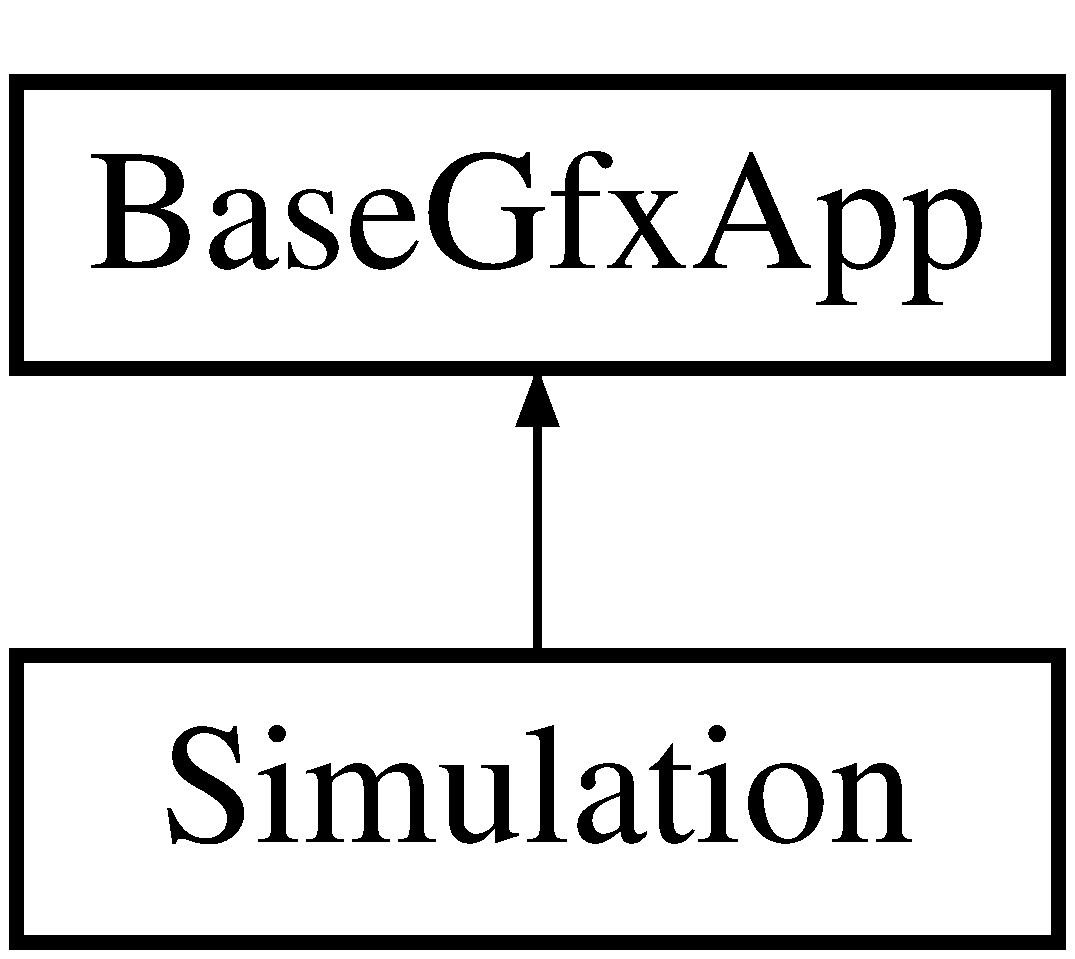
\includegraphics[height=2.000000cm]{classSimulation}
\end{center}
\end{figure}
\subsection*{Public Member Functions}
\begin{DoxyCompactItemize}
\item 
\hyperlink{classSimulation_adcfdbfb67f658534437a17d157099db9}{Simulation} (int argc, char $\ast$argv\mbox{[}$\,$\mbox{]})
\begin{DoxyCompactList}\small\item\em The constructor for the \hyperlink{classSimulation}{Simulation} class. \end{DoxyCompactList}\item 
virtual \hyperlink{classSimulation_a80fad3f57dfaf195a36f7bc49bc88279}{$\sim$\-Simulation} ()
\item 
void \hyperlink{classSimulation_a52eb5c1e4b471bcc38dd71b9432e1840}{init\-Objects} ()
\begin{DoxyCompactList}\small\item\em Adds objects according to configuration. \end{DoxyCompactList}\item 
void \hyperlink{classSimulation_aec7e9ba50cebf0bcb936608450c91916}{try\-Add\-Robot\-Target} ()
\begin{DoxyCompactList}\small\item\em Adds a robot and target to the simulation, or raises an error on failure. \end{DoxyCompactList}\item 
void \hyperlink{classSimulation_a0581c8385e2ab00ee4bda7252ae713e3}{try\-Add\-Robot} ()
\begin{DoxyCompactList}\small\item\em Adds a robot to the simulation, or raises an error on failure. \end{DoxyCompactList}\item 
void \hyperlink{classSimulation_ab8614040d41b38ae0121316d1f0c19fc}{try\-Add\-Stationary\-Light\-Source} ()
\begin{DoxyCompactList}\small\item\em Adds a stationary light to the simulation, or raises an error on failure. \end{DoxyCompactList}\item 
void \hyperlink{classSimulation_a4d569e8e740c702a3a1456944f1461d1}{try\-Add\-Moving\-Light\-Source} ()
\begin{DoxyCompactList}\small\item\em Adds a moving light to the simulation, or raises an error on failure. \end{DoxyCompactList}\item 
void \hyperlink{classSimulation_a1285117bf231d9aa145104256a1cdb36}{try\-Add\-Obstacle} ()
\begin{DoxyCompactList}\small\item\em Adds a obstacle to the simulation, or raises an error on failure. \end{DoxyCompactList}\item 
void \hyperlink{classSimulation_ae5d3e5de317edd69474681812601b2b4}{try\-Remove\-Robot\-Target} ()
\begin{DoxyCompactList}\small\item\em Removes a robot and target from the simulation, or raises an error on failure. \end{DoxyCompactList}\item 
void \hyperlink{classSimulation_a3ea83c539222757b77094aba6a7b92f4}{try\-Remove\-Light\-Source} ()
\begin{DoxyCompactList}\small\item\em Removes a light from the simulation, or raises an error on failure. \end{DoxyCompactList}\item 
void \hyperlink{classSimulation_a9c9922c4e4c4e9a9ceb6ab58adf007ae}{try\-Remove\-Obstacle} ()
\begin{DoxyCompactList}\small\item\em Removes a obstacle from the simulation, or raises an error on failure. \end{DoxyCompactList}\item 
void \hyperlink{classSimulation_ac89e545669001c0f8c9bbbb27a9b15a2}{try\-Open} ()
\begin{DoxyCompactList}\small\item\em Loads a simulation, or raises an error on failure. \end{DoxyCompactList}\item 
void \hyperlink{classSimulation_a46b400f0753d2e434bc82e3824f2d308}{try\-Save} ()
\begin{DoxyCompactList}\small\item\em Saves a simulation, or raises an error on failure. \end{DoxyCompactList}\item 
void \hyperlink{classSimulation_a449dcb7d97dfba99efe770de2f399c31}{display} ()
\begin{DoxyCompactList}\small\item\em Call-\/back function to render all the objects.  This function is called repeatedly from glut, and iterates through the objects and calls their respective display functions. \end{DoxyCompactList}\item 
void \hyperlink{classSimulation_a4938ccecec0e9356cf547ef7bd5bbdf8}{advance} ()
\begin{DoxyCompactList}\small\item\em Call-\/back function to update the positions of all objects.  This function is called repeatedly from glut, and iterates through the objects and calls their respective update\-Position functions. \end{DoxyCompactList}\item 
void \hyperlink{classSimulation_a1607cd18e552ab9f4a6f57d362f7121a}{glui\-Control} (int control\-I\-D)
\begin{DoxyCompactList}\small\item\em Call-\/back function for user input. \end{DoxyCompactList}\item 
void \hyperlink{classSimulation_a786d1ba31d29937f0ac6f3ea88f8a607}{left\-Mouse\-Down} (int x, int y)
\begin{DoxyCompactList}\small\item\em Call-\/back function for mouse click. \end{DoxyCompactList}\item 
void \hyperlink{classSimulation_a62ef254d85017074cd521a5787b5a234}{left\-Mouse\-Up} (int x, int y)
\begin{DoxyCompactList}\small\item\em Call-\/back function for mouse click. \end{DoxyCompactList}\item 
void \hyperlink{classSimulation_a4a8fb0f5c7cff8e747ae11d46653d18b}{middle\-Mouse\-Down} (int x, int y)
\begin{DoxyCompactList}\small\item\em Call-\/back function for mouse click. \end{DoxyCompactList}\item 
void \hyperlink{classSimulation_af942a4554aa7a45b468ea7e5bc2e0c4b}{mouse\-Dragged} (int x, int y)
\begin{DoxyCompactList}\small\item\em Call-\/back function for mouse drag. \end{DoxyCompactList}\item 
void \hyperlink{classSimulation_af2fc2b7caf1b85fb68c82375c3391569}{keyboard} (unsigned char key, int x, int y)
\begin{DoxyCompactList}\small\item\em Call-\/back function keyboard press. \end{DoxyCompactList}\item 
void \hyperlink{classSimulation_ac60b25961b18057239efcb610b5c679f}{keyboard\-Special} (int key, int x, int y)
\begin{DoxyCompactList}\small\item\em Call-\/back function for special keyboard press. \end{DoxyCompactList}\item 
void \hyperlink{classSimulation_adaf59b9b5a544f6214d636632a16d6d4}{start} (int)
\item 
void \hyperlink{classSimulation_a72676ce712a367d4124bf88f4165b7b7}{pause} (int)
\item 
void \hyperlink{classSimulation_aecfee72e6cd12d7b2a847a9c9b0634ec}{resume} (int)
\item 
void \hyperlink{classSimulation_aa35f76e4125149c4bd71b2d870eaa70d}{reset} (int)
\item 
void \hyperlink{classSimulation_ae47fcb172ad1e42adeb91c0a9bc8e1cd}{clear} (int)
\item 
void \hyperlink{classSimulation_a71222e784171f690ec3953de65c4a84c}{random} (int)
\end{DoxyCompactItemize}
\subsection*{Static Public Member Functions}
\begin{DoxyCompactItemize}
\item 
static void \hyperlink{classSimulation_a4fbdc741b91e30e8ae6660e0df440b0f}{s\-\_\-start} (int)
\item 
static void \hyperlink{classSimulation_a5f23f02ab2ff4908179428b679cd35e0}{s\-\_\-pause} (int)
\item 
static void \hyperlink{classSimulation_a488913a8c9940626ae33fbb46fcaa3ba}{s\-\_\-resume} (int)
\item 
static void \hyperlink{classSimulation_a126696e55171934239ad04f8967868a7}{s\-\_\-reset} (int)
\item 
static void \hyperlink{classSimulation_a8155c197bab91873c70265d50e257108}{s\-\_\-clear} (int)
\item 
static void \hyperlink{classSimulation_abaa6fb8813325571348d49ff8f7d63d1}{s\-\_\-random} (int)
\item 
static void \hyperlink{classSimulation_a8809bedf93cf98b14595606702dac2ea}{s\-\_\-add\-Robot\-Target} (int)
\item 
static void \hyperlink{classSimulation_af58dab21fe89ca343e68143663a4c02b}{s\-\_\-add\-Robot} (int)
\item 
static void \hyperlink{classSimulation_a81fd62337fe6091c4a10277f24d3283e}{s\-\_\-add\-Stationary\-Light\-Source} (int)
\item 
static void \hyperlink{classSimulation_a6712136802456306afa232fc50999494}{s\-\_\-add\-Moving\-Light\-Source} (int)
\item 
static void \hyperlink{classSimulation_ae27ff6c795de81dcffe7f6e0e9b2e056}{s\-\_\-add\-Obstacle} (int)
\item 
static void \hyperlink{classSimulation_a2eac6140af57c80832b96f7baeaa1541}{s\-\_\-remove\-Robot\-Target} (int)
\item 
static void \hyperlink{classSimulation_a4582e4be95ed1c5e6d56b9784c6d445d}{s\-\_\-remove\-Light\-Source} (int)
\item 
static void \hyperlink{classSimulation_ace6392d4941964d55dd015d72cd4d329}{s\-\_\-remove\-Obstacle} (int)
\item 
static void \hyperlink{classSimulation_a44d48e7718d802a3f487728088883062}{s\-\_\-remove\-All\-Robot\-Target} (int)
\item 
static void \hyperlink{classSimulation_a4a93430b4e38ab42ad0484068aa8c7ef}{s\-\_\-remove\-All\-Light\-Source} (int)
\item 
static void \hyperlink{classSimulation_a98c4456a49c4b2776376be37e9600ba6}{s\-\_\-remove\-All\-Obstacle} (int)
\item 
static void \hyperlink{classSimulation_a8f8588b5f9f96ab590e89f5635413b09}{s\-\_\-refresh\-Configuration} (int)
\item 
static void \hyperlink{classSimulation_a0ac559574b30698f53597049c90f3c54}{s\-\_\-open} (int)
\item 
static void \hyperlink{classSimulation_a8819e4930c1ff660d8a711390d7cd441}{s\-\_\-save} (int)
\item 
static void \hyperlink{classSimulation_aa517549d904986ed7862125ce22385c1}{s\-\_\-neural\-Network\-File\-Changed} (int)
\end{DoxyCompactItemize}
\subsection*{Additional Inherited Members}


\subsection{Detailed Description}
\hyperlink{classSimulation}{Simulation} class, sets up the G\-U\-I and the drawing environment. 

\subsection{Constructor \& Destructor Documentation}
\hypertarget{classSimulation_adcfdbfb67f658534437a17d157099db9}{\index{Simulation@{Simulation}!Simulation@{Simulation}}
\index{Simulation@{Simulation}!Simulation@{Simulation}}
\subsubsection[{Simulation}]{\setlength{\rightskip}{0pt plus 5cm}Simulation\-::\-Simulation (
\begin{DoxyParamCaption}
\item[{int}]{argc, }
\item[{char $\ast$}]{argv\mbox{[}$\,$\mbox{]}}
\end{DoxyParamCaption}
)}}\label{classSimulation_adcfdbfb67f658534437a17d157099db9}


The constructor for the \hyperlink{classSimulation}{Simulation} class. 


\begin{DoxyParams}{Parameters}
{\em argc} & The number of command-\/line arguments \\
\hline
{\em argv} & The command-\/line arguments \\
\hline
\end{DoxyParams}
\hypertarget{classSimulation_a80fad3f57dfaf195a36f7bc49bc88279}{\index{Simulation@{Simulation}!$\sim$\-Simulation@{$\sim$\-Simulation}}
\index{$\sim$\-Simulation@{$\sim$\-Simulation}!Simulation@{Simulation}}
\subsubsection[{$\sim$\-Simulation}]{\setlength{\rightskip}{0pt plus 5cm}Simulation\-::$\sim$\-Simulation (
\begin{DoxyParamCaption}
{}
\end{DoxyParamCaption}
)\hspace{0.3cm}{\ttfamily [virtual]}}}\label{classSimulation_a80fad3f57dfaf195a36f7bc49bc88279}


\subsection{Member Function Documentation}
\hypertarget{classSimulation_a4938ccecec0e9356cf547ef7bd5bbdf8}{\index{Simulation@{Simulation}!advance@{advance}}
\index{advance@{advance}!Simulation@{Simulation}}
\subsubsection[{advance}]{\setlength{\rightskip}{0pt plus 5cm}void Simulation\-::advance (
\begin{DoxyParamCaption}
{}
\end{DoxyParamCaption}
)\hspace{0.3cm}{\ttfamily [virtual]}}}\label{classSimulation_a4938ccecec0e9356cf547ef7bd5bbdf8}


Call-\/back function to update the positions of all objects.  This function is called repeatedly from glut, and iterates through the objects and calls their respective update\-Position functions. 



Reimplemented from \hyperlink{classBaseGfxApp_a432317fc7c028b2c6702eb2232e85425}{Base\-Gfx\-App}.

\hypertarget{classSimulation_ae47fcb172ad1e42adeb91c0a9bc8e1cd}{\index{Simulation@{Simulation}!clear@{clear}}
\index{clear@{clear}!Simulation@{Simulation}}
\subsubsection[{clear}]{\setlength{\rightskip}{0pt plus 5cm}void Simulation\-::clear (
\begin{DoxyParamCaption}
\item[{int}]{}
\end{DoxyParamCaption}
)}}\label{classSimulation_ae47fcb172ad1e42adeb91c0a9bc8e1cd}
\hypertarget{classSimulation_a449dcb7d97dfba99efe770de2f399c31}{\index{Simulation@{Simulation}!display@{display}}
\index{display@{display}!Simulation@{Simulation}}
\subsubsection[{display}]{\setlength{\rightskip}{0pt plus 5cm}void Simulation\-::display (
\begin{DoxyParamCaption}
{}
\end{DoxyParamCaption}
)\hspace{0.3cm}{\ttfamily [virtual]}}}\label{classSimulation_a449dcb7d97dfba99efe770de2f399c31}


Call-\/back function to render all the objects.  This function is called repeatedly from glut, and iterates through the objects and calls their respective display functions. 



Reimplemented from \hyperlink{classBaseGfxApp_ac8de2d5a955582547af5619b771b4d6d}{Base\-Gfx\-App}.

\hypertarget{classSimulation_a1607cd18e552ab9f4a6f57d362f7121a}{\index{Simulation@{Simulation}!glui\-Control@{glui\-Control}}
\index{glui\-Control@{glui\-Control}!Simulation@{Simulation}}
\subsubsection[{glui\-Control}]{\setlength{\rightskip}{0pt plus 5cm}void Simulation\-::glui\-Control (
\begin{DoxyParamCaption}
\item[{int}]{control\-I\-D}
\end{DoxyParamCaption}
)\hspace{0.3cm}{\ttfamily [virtual]}}}\label{classSimulation_a1607cd18e552ab9f4a6f57d362f7121a}


Call-\/back function for user input. 



Reimplemented from \hyperlink{classBaseGfxApp_a2978a7c358794c67df73b66776b2cef3}{Base\-Gfx\-App}.

\hypertarget{classSimulation_a52eb5c1e4b471bcc38dd71b9432e1840}{\index{Simulation@{Simulation}!init\-Objects@{init\-Objects}}
\index{init\-Objects@{init\-Objects}!Simulation@{Simulation}}
\subsubsection[{init\-Objects}]{\setlength{\rightskip}{0pt plus 5cm}void Simulation\-::init\-Objects (
\begin{DoxyParamCaption}
{}
\end{DoxyParamCaption}
)}}\label{classSimulation_a52eb5c1e4b471bcc38dd71b9432e1840}


Adds objects according to configuration. 

\hypertarget{classSimulation_af2fc2b7caf1b85fb68c82375c3391569}{\index{Simulation@{Simulation}!keyboard@{keyboard}}
\index{keyboard@{keyboard}!Simulation@{Simulation}}
\subsubsection[{keyboard}]{\setlength{\rightskip}{0pt plus 5cm}void Simulation\-::keyboard (
\begin{DoxyParamCaption}
\item[{unsigned char}]{key, }
\item[{int}]{x, }
\item[{int}]{y}
\end{DoxyParamCaption}
)\hspace{0.3cm}{\ttfamily [virtual]}}}\label{classSimulation_af2fc2b7caf1b85fb68c82375c3391569}


Call-\/back function keyboard press. 



Reimplemented from \hyperlink{classBaseGfxApp_a6d91e0cb7a3d48cad33956efe7eb36ca}{Base\-Gfx\-App}.

\hypertarget{classSimulation_ac60b25961b18057239efcb610b5c679f}{\index{Simulation@{Simulation}!keyboard\-Special@{keyboard\-Special}}
\index{keyboard\-Special@{keyboard\-Special}!Simulation@{Simulation}}
\subsubsection[{keyboard\-Special}]{\setlength{\rightskip}{0pt plus 5cm}void Simulation\-::keyboard\-Special (
\begin{DoxyParamCaption}
\item[{int}]{key, }
\item[{int}]{x, }
\item[{int}]{y}
\end{DoxyParamCaption}
)\hspace{0.3cm}{\ttfamily [virtual]}}}\label{classSimulation_ac60b25961b18057239efcb610b5c679f}


Call-\/back function for special keyboard press. 



Reimplemented from \hyperlink{classBaseGfxApp_a345566e62c9e4ec3705ec4d1c4c75f1f}{Base\-Gfx\-App}.

\hypertarget{classSimulation_a786d1ba31d29937f0ac6f3ea88f8a607}{\index{Simulation@{Simulation}!left\-Mouse\-Down@{left\-Mouse\-Down}}
\index{left\-Mouse\-Down@{left\-Mouse\-Down}!Simulation@{Simulation}}
\subsubsection[{left\-Mouse\-Down}]{\setlength{\rightskip}{0pt plus 5cm}void Simulation\-::left\-Mouse\-Down (
\begin{DoxyParamCaption}
\item[{int}]{x, }
\item[{int}]{y}
\end{DoxyParamCaption}
)\hspace{0.3cm}{\ttfamily [virtual]}}}\label{classSimulation_a786d1ba31d29937f0ac6f3ea88f8a607}


Call-\/back function for mouse click. 



Reimplemented from \hyperlink{classBaseGfxApp_aaaccf5a5e923a9465441a5ee712424a8}{Base\-Gfx\-App}.

\hypertarget{classSimulation_a62ef254d85017074cd521a5787b5a234}{\index{Simulation@{Simulation}!left\-Mouse\-Up@{left\-Mouse\-Up}}
\index{left\-Mouse\-Up@{left\-Mouse\-Up}!Simulation@{Simulation}}
\subsubsection[{left\-Mouse\-Up}]{\setlength{\rightskip}{0pt plus 5cm}void Simulation\-::left\-Mouse\-Up (
\begin{DoxyParamCaption}
\item[{int}]{x, }
\item[{int}]{y}
\end{DoxyParamCaption}
)\hspace{0.3cm}{\ttfamily [virtual]}}}\label{classSimulation_a62ef254d85017074cd521a5787b5a234}


Call-\/back function for mouse click. 



Reimplemented from \hyperlink{classBaseGfxApp_a0a2961a932b02b2f9d7d0bb408f6fb51}{Base\-Gfx\-App}.

\hypertarget{classSimulation_a4a8fb0f5c7cff8e747ae11d46653d18b}{\index{Simulation@{Simulation}!middle\-Mouse\-Down@{middle\-Mouse\-Down}}
\index{middle\-Mouse\-Down@{middle\-Mouse\-Down}!Simulation@{Simulation}}
\subsubsection[{middle\-Mouse\-Down}]{\setlength{\rightskip}{0pt plus 5cm}void Simulation\-::middle\-Mouse\-Down (
\begin{DoxyParamCaption}
\item[{int}]{x, }
\item[{int}]{y}
\end{DoxyParamCaption}
)\hspace{0.3cm}{\ttfamily [virtual]}}}\label{classSimulation_a4a8fb0f5c7cff8e747ae11d46653d18b}


Call-\/back function for mouse click. 



Reimplemented from \hyperlink{classBaseGfxApp_a2c98cae9bb5ad1fb1832a6d4812670f8}{Base\-Gfx\-App}.

\hypertarget{classSimulation_af942a4554aa7a45b468ea7e5bc2e0c4b}{\index{Simulation@{Simulation}!mouse\-Dragged@{mouse\-Dragged}}
\index{mouse\-Dragged@{mouse\-Dragged}!Simulation@{Simulation}}
\subsubsection[{mouse\-Dragged}]{\setlength{\rightskip}{0pt plus 5cm}void Simulation\-::mouse\-Dragged (
\begin{DoxyParamCaption}
\item[{int}]{x, }
\item[{int}]{y}
\end{DoxyParamCaption}
)\hspace{0.3cm}{\ttfamily [virtual]}}}\label{classSimulation_af942a4554aa7a45b468ea7e5bc2e0c4b}


Call-\/back function for mouse drag. 



Reimplemented from \hyperlink{classBaseGfxApp_abb23f716dd6612b3a72938e41525d338}{Base\-Gfx\-App}.

\hypertarget{classSimulation_a72676ce712a367d4124bf88f4165b7b7}{\index{Simulation@{Simulation}!pause@{pause}}
\index{pause@{pause}!Simulation@{Simulation}}
\subsubsection[{pause}]{\setlength{\rightskip}{0pt plus 5cm}void Simulation\-::pause (
\begin{DoxyParamCaption}
\item[{int}]{}
\end{DoxyParamCaption}
)}}\label{classSimulation_a72676ce712a367d4124bf88f4165b7b7}
\hypertarget{classSimulation_a71222e784171f690ec3953de65c4a84c}{\index{Simulation@{Simulation}!random@{random}}
\index{random@{random}!Simulation@{Simulation}}
\subsubsection[{random}]{\setlength{\rightskip}{0pt plus 5cm}void Simulation\-::random (
\begin{DoxyParamCaption}
\item[{int}]{}
\end{DoxyParamCaption}
)}}\label{classSimulation_a71222e784171f690ec3953de65c4a84c}
\hypertarget{classSimulation_aa35f76e4125149c4bd71b2d870eaa70d}{\index{Simulation@{Simulation}!reset@{reset}}
\index{reset@{reset}!Simulation@{Simulation}}
\subsubsection[{reset}]{\setlength{\rightskip}{0pt plus 5cm}void Simulation\-::reset (
\begin{DoxyParamCaption}
\item[{int}]{}
\end{DoxyParamCaption}
)}}\label{classSimulation_aa35f76e4125149c4bd71b2d870eaa70d}
\hypertarget{classSimulation_aecfee72e6cd12d7b2a847a9c9b0634ec}{\index{Simulation@{Simulation}!resume@{resume}}
\index{resume@{resume}!Simulation@{Simulation}}
\subsubsection[{resume}]{\setlength{\rightskip}{0pt plus 5cm}void Simulation\-::resume (
\begin{DoxyParamCaption}
\item[{int}]{}
\end{DoxyParamCaption}
)}}\label{classSimulation_aecfee72e6cd12d7b2a847a9c9b0634ec}
\hypertarget{classSimulation_a6712136802456306afa232fc50999494}{\index{Simulation@{Simulation}!s\-\_\-add\-Moving\-Light\-Source@{s\-\_\-add\-Moving\-Light\-Source}}
\index{s\-\_\-add\-Moving\-Light\-Source@{s\-\_\-add\-Moving\-Light\-Source}!Simulation@{Simulation}}
\subsubsection[{s\-\_\-add\-Moving\-Light\-Source}]{\setlength{\rightskip}{0pt plus 5cm}void Simulation\-::s\-\_\-add\-Moving\-Light\-Source (
\begin{DoxyParamCaption}
\item[{int}]{a}
\end{DoxyParamCaption}
)\hspace{0.3cm}{\ttfamily [static]}}}\label{classSimulation_a6712136802456306afa232fc50999494}
\hypertarget{classSimulation_ae27ff6c795de81dcffe7f6e0e9b2e056}{\index{Simulation@{Simulation}!s\-\_\-add\-Obstacle@{s\-\_\-add\-Obstacle}}
\index{s\-\_\-add\-Obstacle@{s\-\_\-add\-Obstacle}!Simulation@{Simulation}}
\subsubsection[{s\-\_\-add\-Obstacle}]{\setlength{\rightskip}{0pt plus 5cm}void Simulation\-::s\-\_\-add\-Obstacle (
\begin{DoxyParamCaption}
\item[{int}]{a}
\end{DoxyParamCaption}
)\hspace{0.3cm}{\ttfamily [static]}}}\label{classSimulation_ae27ff6c795de81dcffe7f6e0e9b2e056}
\hypertarget{classSimulation_af58dab21fe89ca343e68143663a4c02b}{\index{Simulation@{Simulation}!s\-\_\-add\-Robot@{s\-\_\-add\-Robot}}
\index{s\-\_\-add\-Robot@{s\-\_\-add\-Robot}!Simulation@{Simulation}}
\subsubsection[{s\-\_\-add\-Robot}]{\setlength{\rightskip}{0pt plus 5cm}void Simulation\-::s\-\_\-add\-Robot (
\begin{DoxyParamCaption}
\item[{int}]{a}
\end{DoxyParamCaption}
)\hspace{0.3cm}{\ttfamily [static]}}}\label{classSimulation_af58dab21fe89ca343e68143663a4c02b}
\hypertarget{classSimulation_a8809bedf93cf98b14595606702dac2ea}{\index{Simulation@{Simulation}!s\-\_\-add\-Robot\-Target@{s\-\_\-add\-Robot\-Target}}
\index{s\-\_\-add\-Robot\-Target@{s\-\_\-add\-Robot\-Target}!Simulation@{Simulation}}
\subsubsection[{s\-\_\-add\-Robot\-Target}]{\setlength{\rightskip}{0pt plus 5cm}void Simulation\-::s\-\_\-add\-Robot\-Target (
\begin{DoxyParamCaption}
\item[{int}]{a}
\end{DoxyParamCaption}
)\hspace{0.3cm}{\ttfamily [static]}}}\label{classSimulation_a8809bedf93cf98b14595606702dac2ea}
\hypertarget{classSimulation_a81fd62337fe6091c4a10277f24d3283e}{\index{Simulation@{Simulation}!s\-\_\-add\-Stationary\-Light\-Source@{s\-\_\-add\-Stationary\-Light\-Source}}
\index{s\-\_\-add\-Stationary\-Light\-Source@{s\-\_\-add\-Stationary\-Light\-Source}!Simulation@{Simulation}}
\subsubsection[{s\-\_\-add\-Stationary\-Light\-Source}]{\setlength{\rightskip}{0pt plus 5cm}void Simulation\-::s\-\_\-add\-Stationary\-Light\-Source (
\begin{DoxyParamCaption}
\item[{int}]{a}
\end{DoxyParamCaption}
)\hspace{0.3cm}{\ttfamily [static]}}}\label{classSimulation_a81fd62337fe6091c4a10277f24d3283e}
\hypertarget{classSimulation_a8155c197bab91873c70265d50e257108}{\index{Simulation@{Simulation}!s\-\_\-clear@{s\-\_\-clear}}
\index{s\-\_\-clear@{s\-\_\-clear}!Simulation@{Simulation}}
\subsubsection[{s\-\_\-clear}]{\setlength{\rightskip}{0pt plus 5cm}void Simulation\-::s\-\_\-clear (
\begin{DoxyParamCaption}
\item[{int}]{a}
\end{DoxyParamCaption}
)\hspace{0.3cm}{\ttfamily [static]}}}\label{classSimulation_a8155c197bab91873c70265d50e257108}
\hypertarget{classSimulation_aa517549d904986ed7862125ce22385c1}{\index{Simulation@{Simulation}!s\-\_\-neural\-Network\-File\-Changed@{s\-\_\-neural\-Network\-File\-Changed}}
\index{s\-\_\-neural\-Network\-File\-Changed@{s\-\_\-neural\-Network\-File\-Changed}!Simulation@{Simulation}}
\subsubsection[{s\-\_\-neural\-Network\-File\-Changed}]{\setlength{\rightskip}{0pt plus 5cm}void Simulation\-::s\-\_\-neural\-Network\-File\-Changed (
\begin{DoxyParamCaption}
\item[{int}]{a}
\end{DoxyParamCaption}
)\hspace{0.3cm}{\ttfamily [static]}}}\label{classSimulation_aa517549d904986ed7862125ce22385c1}
\hypertarget{classSimulation_a0ac559574b30698f53597049c90f3c54}{\index{Simulation@{Simulation}!s\-\_\-open@{s\-\_\-open}}
\index{s\-\_\-open@{s\-\_\-open}!Simulation@{Simulation}}
\subsubsection[{s\-\_\-open}]{\setlength{\rightskip}{0pt plus 5cm}void Simulation\-::s\-\_\-open (
\begin{DoxyParamCaption}
\item[{int}]{a}
\end{DoxyParamCaption}
)\hspace{0.3cm}{\ttfamily [static]}}}\label{classSimulation_a0ac559574b30698f53597049c90f3c54}
\hypertarget{classSimulation_a5f23f02ab2ff4908179428b679cd35e0}{\index{Simulation@{Simulation}!s\-\_\-pause@{s\-\_\-pause}}
\index{s\-\_\-pause@{s\-\_\-pause}!Simulation@{Simulation}}
\subsubsection[{s\-\_\-pause}]{\setlength{\rightskip}{0pt plus 5cm}void Simulation\-::s\-\_\-pause (
\begin{DoxyParamCaption}
\item[{int}]{a}
\end{DoxyParamCaption}
)\hspace{0.3cm}{\ttfamily [static]}}}\label{classSimulation_a5f23f02ab2ff4908179428b679cd35e0}
\hypertarget{classSimulation_abaa6fb8813325571348d49ff8f7d63d1}{\index{Simulation@{Simulation}!s\-\_\-random@{s\-\_\-random}}
\index{s\-\_\-random@{s\-\_\-random}!Simulation@{Simulation}}
\subsubsection[{s\-\_\-random}]{\setlength{\rightskip}{0pt plus 5cm}void Simulation\-::s\-\_\-random (
\begin{DoxyParamCaption}
\item[{int}]{a}
\end{DoxyParamCaption}
)\hspace{0.3cm}{\ttfamily [static]}}}\label{classSimulation_abaa6fb8813325571348d49ff8f7d63d1}
\hypertarget{classSimulation_a8f8588b5f9f96ab590e89f5635413b09}{\index{Simulation@{Simulation}!s\-\_\-refresh\-Configuration@{s\-\_\-refresh\-Configuration}}
\index{s\-\_\-refresh\-Configuration@{s\-\_\-refresh\-Configuration}!Simulation@{Simulation}}
\subsubsection[{s\-\_\-refresh\-Configuration}]{\setlength{\rightskip}{0pt plus 5cm}void Simulation\-::s\-\_\-refresh\-Configuration (
\begin{DoxyParamCaption}
\item[{int}]{a}
\end{DoxyParamCaption}
)\hspace{0.3cm}{\ttfamily [static]}}}\label{classSimulation_a8f8588b5f9f96ab590e89f5635413b09}
\hypertarget{classSimulation_a4a93430b4e38ab42ad0484068aa8c7ef}{\index{Simulation@{Simulation}!s\-\_\-remove\-All\-Light\-Source@{s\-\_\-remove\-All\-Light\-Source}}
\index{s\-\_\-remove\-All\-Light\-Source@{s\-\_\-remove\-All\-Light\-Source}!Simulation@{Simulation}}
\subsubsection[{s\-\_\-remove\-All\-Light\-Source}]{\setlength{\rightskip}{0pt plus 5cm}void Simulation\-::s\-\_\-remove\-All\-Light\-Source (
\begin{DoxyParamCaption}
\item[{int}]{a}
\end{DoxyParamCaption}
)\hspace{0.3cm}{\ttfamily [static]}}}\label{classSimulation_a4a93430b4e38ab42ad0484068aa8c7ef}
\hypertarget{classSimulation_a98c4456a49c4b2776376be37e9600ba6}{\index{Simulation@{Simulation}!s\-\_\-remove\-All\-Obstacle@{s\-\_\-remove\-All\-Obstacle}}
\index{s\-\_\-remove\-All\-Obstacle@{s\-\_\-remove\-All\-Obstacle}!Simulation@{Simulation}}
\subsubsection[{s\-\_\-remove\-All\-Obstacle}]{\setlength{\rightskip}{0pt plus 5cm}void Simulation\-::s\-\_\-remove\-All\-Obstacle (
\begin{DoxyParamCaption}
\item[{int}]{a}
\end{DoxyParamCaption}
)\hspace{0.3cm}{\ttfamily [static]}}}\label{classSimulation_a98c4456a49c4b2776376be37e9600ba6}
\hypertarget{classSimulation_a44d48e7718d802a3f487728088883062}{\index{Simulation@{Simulation}!s\-\_\-remove\-All\-Robot\-Target@{s\-\_\-remove\-All\-Robot\-Target}}
\index{s\-\_\-remove\-All\-Robot\-Target@{s\-\_\-remove\-All\-Robot\-Target}!Simulation@{Simulation}}
\subsubsection[{s\-\_\-remove\-All\-Robot\-Target}]{\setlength{\rightskip}{0pt plus 5cm}void Simulation\-::s\-\_\-remove\-All\-Robot\-Target (
\begin{DoxyParamCaption}
\item[{int}]{a}
\end{DoxyParamCaption}
)\hspace{0.3cm}{\ttfamily [static]}}}\label{classSimulation_a44d48e7718d802a3f487728088883062}
\hypertarget{classSimulation_a4582e4be95ed1c5e6d56b9784c6d445d}{\index{Simulation@{Simulation}!s\-\_\-remove\-Light\-Source@{s\-\_\-remove\-Light\-Source}}
\index{s\-\_\-remove\-Light\-Source@{s\-\_\-remove\-Light\-Source}!Simulation@{Simulation}}
\subsubsection[{s\-\_\-remove\-Light\-Source}]{\setlength{\rightskip}{0pt plus 5cm}void Simulation\-::s\-\_\-remove\-Light\-Source (
\begin{DoxyParamCaption}
\item[{int}]{a}
\end{DoxyParamCaption}
)\hspace{0.3cm}{\ttfamily [static]}}}\label{classSimulation_a4582e4be95ed1c5e6d56b9784c6d445d}
\hypertarget{classSimulation_ace6392d4941964d55dd015d72cd4d329}{\index{Simulation@{Simulation}!s\-\_\-remove\-Obstacle@{s\-\_\-remove\-Obstacle}}
\index{s\-\_\-remove\-Obstacle@{s\-\_\-remove\-Obstacle}!Simulation@{Simulation}}
\subsubsection[{s\-\_\-remove\-Obstacle}]{\setlength{\rightskip}{0pt plus 5cm}void Simulation\-::s\-\_\-remove\-Obstacle (
\begin{DoxyParamCaption}
\item[{int}]{a}
\end{DoxyParamCaption}
)\hspace{0.3cm}{\ttfamily [static]}}}\label{classSimulation_ace6392d4941964d55dd015d72cd4d329}
\hypertarget{classSimulation_a2eac6140af57c80832b96f7baeaa1541}{\index{Simulation@{Simulation}!s\-\_\-remove\-Robot\-Target@{s\-\_\-remove\-Robot\-Target}}
\index{s\-\_\-remove\-Robot\-Target@{s\-\_\-remove\-Robot\-Target}!Simulation@{Simulation}}
\subsubsection[{s\-\_\-remove\-Robot\-Target}]{\setlength{\rightskip}{0pt plus 5cm}void Simulation\-::s\-\_\-remove\-Robot\-Target (
\begin{DoxyParamCaption}
\item[{int}]{a}
\end{DoxyParamCaption}
)\hspace{0.3cm}{\ttfamily [static]}}}\label{classSimulation_a2eac6140af57c80832b96f7baeaa1541}
\hypertarget{classSimulation_a126696e55171934239ad04f8967868a7}{\index{Simulation@{Simulation}!s\-\_\-reset@{s\-\_\-reset}}
\index{s\-\_\-reset@{s\-\_\-reset}!Simulation@{Simulation}}
\subsubsection[{s\-\_\-reset}]{\setlength{\rightskip}{0pt plus 5cm}void Simulation\-::s\-\_\-reset (
\begin{DoxyParamCaption}
\item[{int}]{a}
\end{DoxyParamCaption}
)\hspace{0.3cm}{\ttfamily [static]}}}\label{classSimulation_a126696e55171934239ad04f8967868a7}
\hypertarget{classSimulation_a488913a8c9940626ae33fbb46fcaa3ba}{\index{Simulation@{Simulation}!s\-\_\-resume@{s\-\_\-resume}}
\index{s\-\_\-resume@{s\-\_\-resume}!Simulation@{Simulation}}
\subsubsection[{s\-\_\-resume}]{\setlength{\rightskip}{0pt plus 5cm}void Simulation\-::s\-\_\-resume (
\begin{DoxyParamCaption}
\item[{int}]{a}
\end{DoxyParamCaption}
)\hspace{0.3cm}{\ttfamily [static]}}}\label{classSimulation_a488913a8c9940626ae33fbb46fcaa3ba}
\hypertarget{classSimulation_a8819e4930c1ff660d8a711390d7cd441}{\index{Simulation@{Simulation}!s\-\_\-save@{s\-\_\-save}}
\index{s\-\_\-save@{s\-\_\-save}!Simulation@{Simulation}}
\subsubsection[{s\-\_\-save}]{\setlength{\rightskip}{0pt plus 5cm}void Simulation\-::s\-\_\-save (
\begin{DoxyParamCaption}
\item[{int}]{a}
\end{DoxyParamCaption}
)\hspace{0.3cm}{\ttfamily [static]}}}\label{classSimulation_a8819e4930c1ff660d8a711390d7cd441}
\hypertarget{classSimulation_a4fbdc741b91e30e8ae6660e0df440b0f}{\index{Simulation@{Simulation}!s\-\_\-start@{s\-\_\-start}}
\index{s\-\_\-start@{s\-\_\-start}!Simulation@{Simulation}}
\subsubsection[{s\-\_\-start}]{\setlength{\rightskip}{0pt plus 5cm}void Simulation\-::s\-\_\-start (
\begin{DoxyParamCaption}
\item[{int}]{a}
\end{DoxyParamCaption}
)\hspace{0.3cm}{\ttfamily [static]}}}\label{classSimulation_a4fbdc741b91e30e8ae6660e0df440b0f}
\hypertarget{classSimulation_adaf59b9b5a544f6214d636632a16d6d4}{\index{Simulation@{Simulation}!start@{start}}
\index{start@{start}!Simulation@{Simulation}}
\subsubsection[{start}]{\setlength{\rightskip}{0pt plus 5cm}void Simulation\-::start (
\begin{DoxyParamCaption}
\item[{int}]{}
\end{DoxyParamCaption}
)}}\label{classSimulation_adaf59b9b5a544f6214d636632a16d6d4}
\hypertarget{classSimulation_a4d569e8e740c702a3a1456944f1461d1}{\index{Simulation@{Simulation}!try\-Add\-Moving\-Light\-Source@{try\-Add\-Moving\-Light\-Source}}
\index{try\-Add\-Moving\-Light\-Source@{try\-Add\-Moving\-Light\-Source}!Simulation@{Simulation}}
\subsubsection[{try\-Add\-Moving\-Light\-Source}]{\setlength{\rightskip}{0pt plus 5cm}void Simulation\-::try\-Add\-Moving\-Light\-Source (
\begin{DoxyParamCaption}
{}
\end{DoxyParamCaption}
)}}\label{classSimulation_a4d569e8e740c702a3a1456944f1461d1}


Adds a moving light to the simulation, or raises an error on failure. 

\hypertarget{classSimulation_a1285117bf231d9aa145104256a1cdb36}{\index{Simulation@{Simulation}!try\-Add\-Obstacle@{try\-Add\-Obstacle}}
\index{try\-Add\-Obstacle@{try\-Add\-Obstacle}!Simulation@{Simulation}}
\subsubsection[{try\-Add\-Obstacle}]{\setlength{\rightskip}{0pt plus 5cm}void Simulation\-::try\-Add\-Obstacle (
\begin{DoxyParamCaption}
{}
\end{DoxyParamCaption}
)}}\label{classSimulation_a1285117bf231d9aa145104256a1cdb36}


Adds a obstacle to the simulation, or raises an error on failure. 

\hypertarget{classSimulation_a0581c8385e2ab00ee4bda7252ae713e3}{\index{Simulation@{Simulation}!try\-Add\-Robot@{try\-Add\-Robot}}
\index{try\-Add\-Robot@{try\-Add\-Robot}!Simulation@{Simulation}}
\subsubsection[{try\-Add\-Robot}]{\setlength{\rightskip}{0pt plus 5cm}void Simulation\-::try\-Add\-Robot (
\begin{DoxyParamCaption}
{}
\end{DoxyParamCaption}
)}}\label{classSimulation_a0581c8385e2ab00ee4bda7252ae713e3}


Adds a robot to the simulation, or raises an error on failure. 

\hypertarget{classSimulation_aec7e9ba50cebf0bcb936608450c91916}{\index{Simulation@{Simulation}!try\-Add\-Robot\-Target@{try\-Add\-Robot\-Target}}
\index{try\-Add\-Robot\-Target@{try\-Add\-Robot\-Target}!Simulation@{Simulation}}
\subsubsection[{try\-Add\-Robot\-Target}]{\setlength{\rightskip}{0pt plus 5cm}void Simulation\-::try\-Add\-Robot\-Target (
\begin{DoxyParamCaption}
{}
\end{DoxyParamCaption}
)}}\label{classSimulation_aec7e9ba50cebf0bcb936608450c91916}


Adds a robot and target to the simulation, or raises an error on failure. 

\hypertarget{classSimulation_ab8614040d41b38ae0121316d1f0c19fc}{\index{Simulation@{Simulation}!try\-Add\-Stationary\-Light\-Source@{try\-Add\-Stationary\-Light\-Source}}
\index{try\-Add\-Stationary\-Light\-Source@{try\-Add\-Stationary\-Light\-Source}!Simulation@{Simulation}}
\subsubsection[{try\-Add\-Stationary\-Light\-Source}]{\setlength{\rightskip}{0pt plus 5cm}void Simulation\-::try\-Add\-Stationary\-Light\-Source (
\begin{DoxyParamCaption}
{}
\end{DoxyParamCaption}
)}}\label{classSimulation_ab8614040d41b38ae0121316d1f0c19fc}


Adds a stationary light to the simulation, or raises an error on failure. 

\hypertarget{classSimulation_ac89e545669001c0f8c9bbbb27a9b15a2}{\index{Simulation@{Simulation}!try\-Open@{try\-Open}}
\index{try\-Open@{try\-Open}!Simulation@{Simulation}}
\subsubsection[{try\-Open}]{\setlength{\rightskip}{0pt plus 5cm}void Simulation\-::try\-Open (
\begin{DoxyParamCaption}
{}
\end{DoxyParamCaption}
)}}\label{classSimulation_ac89e545669001c0f8c9bbbb27a9b15a2}


Loads a simulation, or raises an error on failure. 

\hypertarget{classSimulation_a3ea83c539222757b77094aba6a7b92f4}{\index{Simulation@{Simulation}!try\-Remove\-Light\-Source@{try\-Remove\-Light\-Source}}
\index{try\-Remove\-Light\-Source@{try\-Remove\-Light\-Source}!Simulation@{Simulation}}
\subsubsection[{try\-Remove\-Light\-Source}]{\setlength{\rightskip}{0pt plus 5cm}void Simulation\-::try\-Remove\-Light\-Source (
\begin{DoxyParamCaption}
{}
\end{DoxyParamCaption}
)}}\label{classSimulation_a3ea83c539222757b77094aba6a7b92f4}


Removes a light from the simulation, or raises an error on failure. 

\hypertarget{classSimulation_a9c9922c4e4c4e9a9ceb6ab58adf007ae}{\index{Simulation@{Simulation}!try\-Remove\-Obstacle@{try\-Remove\-Obstacle}}
\index{try\-Remove\-Obstacle@{try\-Remove\-Obstacle}!Simulation@{Simulation}}
\subsubsection[{try\-Remove\-Obstacle}]{\setlength{\rightskip}{0pt plus 5cm}void Simulation\-::try\-Remove\-Obstacle (
\begin{DoxyParamCaption}
{}
\end{DoxyParamCaption}
)}}\label{classSimulation_a9c9922c4e4c4e9a9ceb6ab58adf007ae}


Removes a obstacle from the simulation, or raises an error on failure. 

\hypertarget{classSimulation_ae5d3e5de317edd69474681812601b2b4}{\index{Simulation@{Simulation}!try\-Remove\-Robot\-Target@{try\-Remove\-Robot\-Target}}
\index{try\-Remove\-Robot\-Target@{try\-Remove\-Robot\-Target}!Simulation@{Simulation}}
\subsubsection[{try\-Remove\-Robot\-Target}]{\setlength{\rightskip}{0pt plus 5cm}void Simulation\-::try\-Remove\-Robot\-Target (
\begin{DoxyParamCaption}
{}
\end{DoxyParamCaption}
)}}\label{classSimulation_ae5d3e5de317edd69474681812601b2b4}


Removes a robot and target from the simulation, or raises an error on failure. 

\hypertarget{classSimulation_a46b400f0753d2e434bc82e3824f2d308}{\index{Simulation@{Simulation}!try\-Save@{try\-Save}}
\index{try\-Save@{try\-Save}!Simulation@{Simulation}}
\subsubsection[{try\-Save}]{\setlength{\rightskip}{0pt plus 5cm}void Simulation\-::try\-Save (
\begin{DoxyParamCaption}
{}
\end{DoxyParamCaption}
)}}\label{classSimulation_a46b400f0753d2e434bc82e3824f2d308}


Saves a simulation, or raises an error on failure. 



The documentation for this class was generated from the following files\-:\begin{DoxyCompactItemize}
\item 
\hyperlink{Simulation_8h}{Simulation.\-h}\item 
\hyperlink{Simulation_8cpp}{Simulation.\-cpp}\end{DoxyCompactItemize}

\hypertarget{classTarget}{\section{Target Class Reference}
\label{classTarget}\index{Target@{Target}}
}


\hyperlink{classTarget}{Target} for the robot to seek.  




{\ttfamily \#include $<$Target.\-h$>$}

Inheritance diagram for Target\-:\begin{figure}[H]
\begin{center}
\leavevmode
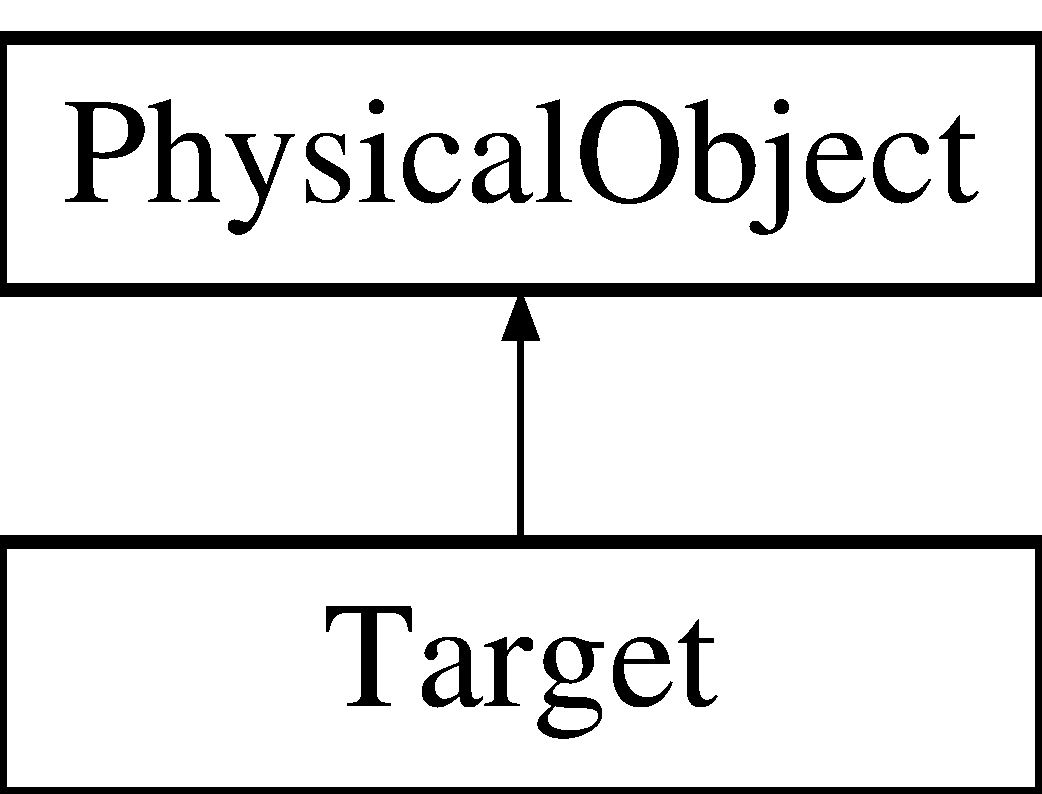
\includegraphics[height=2.000000cm]{classTarget}
\end{center}
\end{figure}
\subsection*{Public Member Functions}
\begin{DoxyCompactItemize}
\item 
\hyperlink{classTarget_a7008d6752ce64f82e56aae6ea6c2bb65}{Target} ()
\item 
\hyperlink{classTarget_a21429bfdca0f6c969f3a65792d56ac76}{Target} (int radius, \hyperlink{structColor}{Color} color, int target\-Num=\hyperlink{PhysicalObject_8h_a842c5e2e69277690b064bf363c017980a09aa9e75617e9d8719738ca163c09137}{T\-A\-R\-G\-E\-T})
\item 
\hyperlink{classTarget_a13cc903b7de80d6a7cfb9d7f3d3a8731}{Target} (int max\-Radius, int min\-Radius, \hyperlink{structColor}{Color} color, int target\-Num=\hyperlink{PhysicalObject_8h_a842c5e2e69277690b064bf363c017980a09aa9e75617e9d8719738ca163c09137}{T\-A\-R\-G\-E\-T})
\item 
\hyperlink{classTarget_a727a453692ead8379b7fc8befe60323e}{Target} (int radius, \hyperlink{structLocation}{Location} loc, \hyperlink{structColor}{Color} color, int target\-Num=\hyperlink{PhysicalObject_8h_a842c5e2e69277690b064bf363c017980a09aa9e75617e9d8719738ca163c09137}{T\-A\-R\-G\-E\-T})
\item 
bool \hyperlink{classTarget_a04dcb816902d80f21c83ed65d44c7bed}{handle\-Collision} (int other\-Id, bool was\-Hit)
\item 
\hyperlink{classTarget_a18102a6c58a268fb1466771463fdc9b3}{$\sim$\-Target} ()
\end{DoxyCompactItemize}
\subsection*{Additional Inherited Members}


\subsection{Detailed Description}
\hyperlink{classTarget}{Target} for the robot to seek. 

\subsection{Constructor \& Destructor Documentation}
\hypertarget{classTarget_a7008d6752ce64f82e56aae6ea6c2bb65}{\index{Target@{Target}!Target@{Target}}
\index{Target@{Target}!Target@{Target}}
\subsubsection[{Target}]{\setlength{\rightskip}{0pt plus 5cm}Target\-::\-Target (
\begin{DoxyParamCaption}
{}
\end{DoxyParamCaption}
)}}\label{classTarget_a7008d6752ce64f82e56aae6ea6c2bb65}
\hypertarget{classTarget_a21429bfdca0f6c969f3a65792d56ac76}{\index{Target@{Target}!Target@{Target}}
\index{Target@{Target}!Target@{Target}}
\subsubsection[{Target}]{\setlength{\rightskip}{0pt plus 5cm}Target\-::\-Target (
\begin{DoxyParamCaption}
\item[{int}]{radius, }
\item[{{\bf Color}}]{color, }
\item[{int}]{target\-Num = {\ttfamily {\bf T\-A\-R\-G\-E\-T}}}
\end{DoxyParamCaption}
)}}\label{classTarget_a21429bfdca0f6c969f3a65792d56ac76}
\hypertarget{classTarget_a13cc903b7de80d6a7cfb9d7f3d3a8731}{\index{Target@{Target}!Target@{Target}}
\index{Target@{Target}!Target@{Target}}
\subsubsection[{Target}]{\setlength{\rightskip}{0pt plus 5cm}Target\-::\-Target (
\begin{DoxyParamCaption}
\item[{int}]{max\-Radius, }
\item[{int}]{min\-Radius, }
\item[{{\bf Color}}]{color, }
\item[{int}]{target\-Num = {\ttfamily {\bf T\-A\-R\-G\-E\-T}}}
\end{DoxyParamCaption}
)}}\label{classTarget_a13cc903b7de80d6a7cfb9d7f3d3a8731}
\hypertarget{classTarget_a727a453692ead8379b7fc8befe60323e}{\index{Target@{Target}!Target@{Target}}
\index{Target@{Target}!Target@{Target}}
\subsubsection[{Target}]{\setlength{\rightskip}{0pt plus 5cm}Target\-::\-Target (
\begin{DoxyParamCaption}
\item[{int}]{radius, }
\item[{{\bf Location}}]{loc, }
\item[{{\bf Color}}]{color, }
\item[{int}]{target\-Num = {\ttfamily {\bf T\-A\-R\-G\-E\-T}}}
\end{DoxyParamCaption}
)}}\label{classTarget_a727a453692ead8379b7fc8befe60323e}
\hypertarget{classTarget_a18102a6c58a268fb1466771463fdc9b3}{\index{Target@{Target}!$\sim$\-Target@{$\sim$\-Target}}
\index{$\sim$\-Target@{$\sim$\-Target}!Target@{Target}}
\subsubsection[{$\sim$\-Target}]{\setlength{\rightskip}{0pt plus 5cm}Target\-::$\sim$\-Target (
\begin{DoxyParamCaption}
{}
\end{DoxyParamCaption}
)}}\label{classTarget_a18102a6c58a268fb1466771463fdc9b3}
This is the class destructor. 

\subsection{Member Function Documentation}
\hypertarget{classTarget_a04dcb816902d80f21c83ed65d44c7bed}{\index{Target@{Target}!handle\-Collision@{handle\-Collision}}
\index{handle\-Collision@{handle\-Collision}!Target@{Target}}
\subsubsection[{handle\-Collision}]{\setlength{\rightskip}{0pt plus 5cm}bool Target\-::handle\-Collision (
\begin{DoxyParamCaption}
\item[{int}]{other\-Id, }
\item[{bool}]{was\-Hit}
\end{DoxyParamCaption}
)\hspace{0.3cm}{\ttfamily [virtual]}}}\label{classTarget_a04dcb816902d80f21c83ed65d44c7bed}
\begin{DoxyAuthor}{Author}
Lucas Kramer This function gives \hyperlink{classTarget}{Target} an appropriate reaction when a collision occurs. 
\end{DoxyAuthor}

\begin{DoxyParams}{Parameters}
{\em other\-Id} & id of the object that it collides with \\
\hline
{\em was\-Hit} & tells if the object was hit previously \\
\hline
\end{DoxyParams}


Implements \hyperlink{classPhysicalObject_a400ba3545479ebbf8b1b4a046906e562}{Physical\-Object}.



The documentation for this class was generated from the following files\-:\begin{DoxyCompactItemize}
\item 
\hyperlink{Target_8h}{Target.\-h}\item 
\hyperlink{Target_8cpp}{Target.\-cpp}\end{DoxyCompactItemize}

\chapter{File Documentation}
\hypertarget{artist_8cpp}{\section{artist.\-cpp File Reference}
\label{artist_8cpp}\index{artist.\-cpp@{artist.\-cpp}}
}
{\ttfamily \#include \char`\"{}Color.\-h\char`\"{}}\\*
{\ttfamily \#include \char`\"{}artist.\-h\char`\"{}}\\*
{\ttfamily \#include \char`\"{}configuration.\-h\char`\"{}}\\*
{\ttfamily \#include $<$G\-L/glut.\-h$>$}\\*
{\ttfamily \#include $<$G\-L/glu.\-h$>$}\\*
{\ttfamily \#include $<$math.\-h$>$}\\*
\subsection*{Namespaces}
\begin{DoxyCompactItemize}
\item 
\hyperlink{namespaceartist}{artist}
\begin{DoxyCompactList}\small\item\em graphical commands \end{DoxyCompactList}\end{DoxyCompactItemize}
\subsection*{Macros}
\begin{DoxyCompactItemize}
\item 
\#define \hyperlink{artist_8cpp_a525335710b53cb064ca56b936120431e}{\-\_\-\-U\-S\-E\-\_\-\-M\-A\-T\-H\-\_\-\-D\-E\-F\-I\-N\-E\-S}
\end{DoxyCompactItemize}
\subsection*{Functions}
\begin{DoxyCompactItemize}
\item 
void \hyperlink{namespaceartist_a1448f39368e6eb1c1c070aba00767141}{artist\-::draw\-Object} (\hyperlink{structLocation}{Location} loc, int radius, \hyperlink{structColor}{Color} color)
\item 
void \hyperlink{namespaceartist_a078dbf47b29eb68f94c0fb4bcf075923}{artist\-::debug\-Arrow} (\hyperlink{structLocation}{Location} loc, int orientation)
\item 
void \hyperlink{namespaceartist_a54b058b55aa1c86eade343d055a91abc}{artist\-::draw\-Light} (\hyperlink{structLocation}{Location} loc, int radius, \hyperlink{structColor}{Color} color)
\item 
void \hyperlink{namespaceartist_acdb1a447e5436ee484f84c8dd64410ee}{artist\-::draw\-Obstacle} (\hyperlink{structLocation}{Location} loc, int radius)
\item 
void \hyperlink{namespaceartist_a3396363108746338a9f8d0d3bf334c09}{artist\-::draw\-Sensor} (\hyperlink{structLocation}{Location} loc, int orientation, int angle, float intensity)
\item 
void \hyperlink{namespaceartist_aa60b5844db3fb3073387b39ba19ea0ad}{artist\-::draw\-Robot} (\hyperlink{structLocation}{Location} loc, int radius, int orientation, \hyperlink{structColor}{Color} color, \hyperlink{structColor}{Color} line\-Color)
\end{DoxyCompactItemize}


\subsection{Macro Definition Documentation}
\hypertarget{artist_8cpp_a525335710b53cb064ca56b936120431e}{\index{artist.\-cpp@{artist.\-cpp}!\-\_\-\-U\-S\-E\-\_\-\-M\-A\-T\-H\-\_\-\-D\-E\-F\-I\-N\-E\-S@{\-\_\-\-U\-S\-E\-\_\-\-M\-A\-T\-H\-\_\-\-D\-E\-F\-I\-N\-E\-S}}
\index{\-\_\-\-U\-S\-E\-\_\-\-M\-A\-T\-H\-\_\-\-D\-E\-F\-I\-N\-E\-S@{\-\_\-\-U\-S\-E\-\_\-\-M\-A\-T\-H\-\_\-\-D\-E\-F\-I\-N\-E\-S}!artist.cpp@{artist.\-cpp}}
\subsubsection[{\-\_\-\-U\-S\-E\-\_\-\-M\-A\-T\-H\-\_\-\-D\-E\-F\-I\-N\-E\-S}]{\setlength{\rightskip}{0pt plus 5cm}\#define \-\_\-\-U\-S\-E\-\_\-\-M\-A\-T\-H\-\_\-\-D\-E\-F\-I\-N\-E\-S}}\label{artist_8cpp_a525335710b53cb064ca56b936120431e}

\hypertarget{artist_8h}{\section{artist.\-h File Reference}
\label{artist_8h}\index{artist.\-h@{artist.\-h}}
}


A namespace for Open\-G\-L graphical functions.  


{\ttfamily \#include \char`\"{}Color.\-h\char`\"{}}\\*
{\ttfamily \#include \char`\"{}Location.\-h\char`\"{}}\\*
\subsection*{Namespaces}
\begin{DoxyCompactItemize}
\item 
\hyperlink{namespaceartist}{artist}
\begin{DoxyCompactList}\small\item\em graphical commands \end{DoxyCompactList}\end{DoxyCompactItemize}
\subsection*{Functions}
\begin{DoxyCompactItemize}
\item 
void \hyperlink{namespaceartist_a078dbf47b29eb68f94c0fb4bcf075923}{artist\-::debug\-Arrow} (\hyperlink{structLocation}{Location} loc, int orientation)
\item 
void \hyperlink{namespaceartist_a1448f39368e6eb1c1c070aba00767141}{artist\-::draw\-Object} (\hyperlink{structLocation}{Location} loc, int radius, \hyperlink{structColor}{Color} color)
\item 
void \hyperlink{namespaceartist_a54b058b55aa1c86eade343d055a91abc}{artist\-::draw\-Light} (\hyperlink{structLocation}{Location} loc, int radius, \hyperlink{structColor}{Color} color)
\item 
void \hyperlink{namespaceartist_acdb1a447e5436ee484f84c8dd64410ee}{artist\-::draw\-Obstacle} (\hyperlink{structLocation}{Location} loc, int radius)
\item 
void \hyperlink{namespaceartist_a3396363108746338a9f8d0d3bf334c09}{artist\-::draw\-Sensor} (\hyperlink{structLocation}{Location} loc, int orientation, int angle, float intensity)
\item 
void \hyperlink{namespaceartist_aa60b5844db3fb3073387b39ba19ea0ad}{artist\-::draw\-Robot} (\hyperlink{structLocation}{Location} loc, int radius, int orientation, \hyperlink{structColor}{Color} color, \hyperlink{structColor}{Color} line\-Color)
\end{DoxyCompactItemize}


\subsection{Detailed Description}
A namespace for Open\-G\-L graphical functions. \begin{DoxyAuthor}{Author}
Carl Bahn  Lucas Kramer 
\end{DoxyAuthor}

\hypertarget{BaseGfxApp_8cpp}{\section{Base\-Gfx\-App.\-cpp File Reference}
\label{BaseGfxApp_8cpp}\index{Base\-Gfx\-App.\-cpp@{Base\-Gfx\-App.\-cpp}}
}


Implementation of \hyperlink{classBaseGfxApp}{Base\-Gfx\-App}.  


{\ttfamily \#include \char`\"{}Base\-Gfx\-App.\-h\char`\"{}}\\*


\subsection{Detailed Description}
Implementation of \hyperlink{classBaseGfxApp}{Base\-Gfx\-App}. \begin{DoxyAuthor}{Author}
C\-Sci3081 Guru  Carl Bahn, Lucas Kramer 
\end{DoxyAuthor}

\hypertarget{BaseGfxApp_8h}{\section{Base\-Gfx\-App.\-h File Reference}
\label{BaseGfxApp_8h}\index{Base\-Gfx\-App.\-h@{Base\-Gfx\-App.\-h}}
}


The basic application class for C\-Sci-\/3081 project. Uses G\-L\-U\-T and G\-L\-U\-I and wraps them in a nice C++ interface.  


{\ttfamily \#include $<$string$>$}\\*
{\ttfamily \#include $<$iostream$>$}\\*
{\ttfamily \#include $<$assert.\-h$>$}\\*
{\ttfamily \#include $<$G\-L/glui.\-h$>$}\\*
\subsection*{Classes}
\begin{DoxyCompactItemize}
\item 
class \hyperlink{classBaseGfxApp}{Base\-Gfx\-App}
\begin{DoxyCompactList}\small\item\em Graphics driver class. \end{DoxyCompactList}\end{DoxyCompactItemize}


\subsection{Detailed Description}
The basic application class for C\-Sci-\/3081 project. Uses G\-L\-U\-T and G\-L\-U\-I and wraps them in a nice C++ interface. \begin{DoxyAuthor}{Author}
C\-Sci3081 Guru  Carl Bahn, Lucas Kramer 
\end{DoxyAuthor}

\hypertarget{Color_8cpp}{\section{Color.\-cpp File Reference}
\label{Color_8cpp}\index{Color.\-cpp@{Color.\-cpp}}
}


Utility functions for handling color.  


{\ttfamily \#include \char`\"{}Color.\-h\char`\"{}}\\*
{\ttfamily \#include \char`\"{}configuration.\-h\char`\"{}}\\*
{\ttfamily \#include $<$iostream$>$}\\*
{\ttfamily \#include $<$cstdlib$>$}\\*
{\ttfamily \#include $<$math.\-h$>$}\\*


\subsection{Detailed Description}
Utility functions for handling color. \begin{DoxyAuthor}{Author}
Carl Bahn  Lucas Kramer 
\end{DoxyAuthor}

\hypertarget{Color_8h}{\section{Color.\-h File Reference}
\label{Color_8h}\index{Color.\-h@{Color.\-h}}
}


Definintions for representing any hexedecimal color.  


{\ttfamily \#include $<$iostream$>$}\\*
\subsection*{Classes}
\begin{DoxyCompactItemize}
\item 
struct \hyperlink{structColor}{Color}
\begin{DoxyCompactList}\small\item\em This struct holds the representation of a color. \end{DoxyCompactList}\end{DoxyCompactItemize}
\subsection*{Macros}
\begin{DoxyCompactItemize}
\item 
\#define \hyperlink{Color_8h_a34de2dea1461260a1e294eee2dae69b9}{G\-E\-T\-\_\-\-C\-O\-L\-O\-R}(C\-O\-L\-O\-R\-\_\-\-V\-A\-R)
\end{DoxyCompactItemize}
\subsection*{Typedefs}
\begin{DoxyCompactItemize}
\item 
typedef struct \hyperlink{structColor}{Color} \hyperlink{Color_8h_a0af5129fc90cfaec2f17f58fb0fb9686}{Color}
\begin{DoxyCompactList}\small\item\em This struct holds the representation of a color. \end{DoxyCompactList}\end{DoxyCompactItemize}


\subsection{Detailed Description}
Definintions for representing any hexedecimal color. \begin{DoxyAuthor}{Author}
Lucas Kramer 
\end{DoxyAuthor}


\subsection{Macro Definition Documentation}
\hypertarget{Color_8h_a34de2dea1461260a1e294eee2dae69b9}{\index{Color.\-h@{Color.\-h}!G\-E\-T\-\_\-\-C\-O\-L\-O\-R@{G\-E\-T\-\_\-\-C\-O\-L\-O\-R}}
\index{G\-E\-T\-\_\-\-C\-O\-L\-O\-R@{G\-E\-T\-\_\-\-C\-O\-L\-O\-R}!Color.h@{Color.\-h}}
\subsubsection[{G\-E\-T\-\_\-\-C\-O\-L\-O\-R}]{\setlength{\rightskip}{0pt plus 5cm}\#define G\-E\-T\-\_\-\-C\-O\-L\-O\-R(
\begin{DoxyParamCaption}
\item[{}]{C\-O\-L\-O\-R\-\_\-\-V\-A\-R}
\end{DoxyParamCaption}
)}}\label{Color_8h_a34de2dea1461260a1e294eee2dae69b9}
{\bfseries Value\-:}
\begin{DoxyCode}
(GET\_BOOL(\textcolor{stringliteral}{"USE\_HEX\_COLORS"})?                          \hyperlink{Color_8h_a0af5129fc90cfaec2f17f58fb0fb9686}{\(\backslash\)}
\hyperlink{Color_8h_a0af5129fc90cfaec2f17f58fb0fb9686}{   Color}(GET\_INT(COLOR\_VAR \textcolor{stringliteral}{"\_HEX"})) :                   \(\backslash\)
   \hyperlink{structColor}{Color}(GET\_CHAR(COLOR\_VAR)))
\end{DoxyCode}


\subsection{Typedef Documentation}
\hypertarget{Color_8h_a0af5129fc90cfaec2f17f58fb0fb9686}{\index{Color.\-h@{Color.\-h}!Color@{Color}}
\index{Color@{Color}!Color.h@{Color.\-h}}
\subsubsection[{Color}]{\setlength{\rightskip}{0pt plus 5cm}typedef struct {\bf Color}  {\bf Color}}}\label{Color_8h_a0af5129fc90cfaec2f17f58fb0fb9686}


This struct holds the representation of a color. 

Each field is a float value that shoult be between 0 and 1. This allows a direct translation from hex colors, with each field being the hex R\-G\-B value / 255. 
\hypertarget{ComplexRobot_8cpp}{\section{Complex\-Robot.\-cpp File Reference}
\label{ComplexRobot_8cpp}\index{Complex\-Robot.\-cpp@{Complex\-Robot.\-cpp}}
}


The representation of a robot within the simulation.  


{\ttfamily \#include $<$G\-L/glu.\-h$>$}\\*
{\ttfamily \#include $<$G\-L/glut.\-h$>$}\\*
{\ttfamily \#include $<$stdexcept$>$}\\*
{\ttfamily \#include \char`\"{}environment.\-h\char`\"{}}\\*
{\ttfamily \#include \char`\"{}Robot.\-h\char`\"{}}\\*
{\ttfamily \#include \char`\"{}Complex\-Robot.\-h\char`\"{}}\\*
{\ttfamily \#include \char`\"{}configuration.\-h\char`\"{}}\\*


\subsection{Detailed Description}
The representation of a robot within the simulation. \begin{DoxyAuthor}{Author}
Lucas Kramer 
\end{DoxyAuthor}

\hypertarget{ComplexRobot_8h}{\section{Complex\-Robot.\-h File Reference}
\label{ComplexRobot_8h}\index{Complex\-Robot.\-h@{Complex\-Robot.\-h}}
}


The representation of a robot within the simulation.  


{\ttfamily \#include \char`\"{}Physical\-Object.\-h\char`\"{}}\\*
{\ttfamily \#include \char`\"{}Robot.\-h\char`\"{}}\\*
{\ttfamily \#include \char`\"{}Sensor.\-h\char`\"{}}\\*
{\ttfamily \#include \char`\"{}configuration.\-h\char`\"{}}\\*
\subsection*{Classes}
\begin{DoxyCompactItemize}
\item 
class \hyperlink{classComplexRobot}{Complex\-Robot}
\begin{DoxyCompactList}\small\item\em A complex robot with configurable feedback from all sensors. \end{DoxyCompactList}\end{DoxyCompactItemize}


\subsection{Detailed Description}
The representation of a robot within the simulation. \begin{DoxyAuthor}{Author}
Lucas Kramer 
\end{DoxyAuthor}

\hypertarget{environment_8cpp}{\section{environment.\-cpp File Reference}
\label{environment_8cpp}\index{environment.\-cpp@{environment.\-cpp}}
}
{\ttfamily \#include \char`\"{}Physical\-Object.\-h\char`\"{}}\\*
{\ttfamily \#include \char`\"{}environment.\-h\char`\"{}}\\*
{\ttfamily \#include \char`\"{}configuration.\-h\char`\"{}}\\*
{\ttfamily \#include $<$iostream$>$}\\*
{\ttfamily \#include $<$math.\-h$>$}\\*
\subsection*{Functions}
\begin{DoxyCompactItemize}
\item 
bool \hyperlink{environment_8cpp_abf64bd28a758ad54f0fd6c028284d0ca}{is\-Touching} (\hyperlink{structLocation}{Location} l1, int r1, \hyperlink{structLocation}{Location} l2, int r2)
\end{DoxyCompactItemize}


\subsection{Function Documentation}
\hypertarget{environment_8cpp_abf64bd28a758ad54f0fd6c028284d0ca}{\index{environment.\-cpp@{environment.\-cpp}!is\-Touching@{is\-Touching}}
\index{is\-Touching@{is\-Touching}!environment.cpp@{environment.\-cpp}}
\subsubsection[{is\-Touching}]{\setlength{\rightskip}{0pt plus 5cm}bool is\-Touching (
\begin{DoxyParamCaption}
\item[{{\bf Location}}]{l1, }
\item[{int}]{r1, }
\item[{{\bf Location}}]{l2, }
\item[{int}]{r2}
\end{DoxyParamCaption}
)}}\label{environment_8cpp_abf64bd28a758ad54f0fd6c028284d0ca}
Checks if two objects specified by their Locations and radii \begin{DoxyReturn}{Returns}
a boolean value that is true when objects are overlapping 
\end{DoxyReturn}

\hypertarget{environment_8h}{\section{environment.\-h File Reference}
\label{environment_8h}\index{environment.\-h@{environment.\-h}}
}
{\ttfamily \#include \char`\"{}Location.\-h\char`\"{}}\\*
{\ttfamily \#include \char`\"{}configuration.\-h\char`\"{}}\\*
{\ttfamily \#include $<$unordered\-\_\-map$>$}\\*
{\ttfamily \#include $<$vector$>$}\\*
{\ttfamily \#include $<$mutex$>$}\\*
{\ttfamily \#include $<$stdexcept$>$}\\*
\subsection*{Classes}
\begin{DoxyCompactItemize}
\item 
class \hyperlink{classObjectIterator}{Object\-Iterator}
\begin{DoxyCompactList}\small\item\em \hyperlink{classObjectIterator}{Object\-Iterator} class, a simple iterator for the object in environment. \end{DoxyCompactList}\item 
class \hyperlink{classNoOpenLocationException}{No\-Open\-Location\-Exception}
\begin{DoxyCompactList}\small\item\em An exception to be thrown when an open \hyperlink{structLocation}{Location} cannot be found. \end{DoxyCompactList}\end{DoxyCompactItemize}
\subsection*{Namespaces}
\begin{DoxyCompactItemize}
\item 
\hyperlink{namespaceenvironment}{environment}
\begin{DoxyCompactList}\small\item\em environment namespace, handles all the objects as a group. Also manages object ids and collision detection \end{DoxyCompactList}\end{DoxyCompactItemize}
\subsection*{Typedefs}
\begin{DoxyCompactItemize}
\item 
typedef \hyperlink{classObjectIterator}{Object\-Iterator} \hyperlink{namespaceenvironment_a3a7a388d4b4ceb0a34bf0c72579780e1}{environment\-::object\-Iterator}
\end{DoxyCompactItemize}
\subsection*{Functions}
\begin{DoxyCompactItemize}
\item 
int \hyperlink{namespaceenvironment_ae9ecf3e6b007d1c73cf18594d659b255}{environment\-::add\-Object} (\hyperlink{classPhysicalObject}{Physical\-Object} $\ast$object)
\begin{DoxyCompactList}\small\item\em Adds an object to the environment. \end{DoxyCompactList}\item 
void \hyperlink{namespaceenvironment_a26801958350a15098c590192c8dcd751}{environment\-::remove\-Object} (int id)
\begin{DoxyCompactList}\small\item\em Removes an object from the environment. \end{DoxyCompactList}\item 
void \hyperlink{namespaceenvironment_a883864c5c3c7f8ca4954781dae04bc11}{environment\-::clear} ()
\begin{DoxyCompactList}\small\item\em Removes all objects from the environment and resets the id counter. \end{DoxyCompactList}\item 
unsigned \hyperlink{namespaceenvironment_a450984ea6790ba4e65e004133fb26c9c}{environment\-::get\-Num\-Objects} ()
\begin{DoxyCompactList}\small\item\em Gets the number of objects in environment. \end{DoxyCompactList}\item 
\hyperlink{classPhysicalObject}{Physical\-Object} $\ast$ \hyperlink{namespaceenvironment_a63ac0eb5daa2876cd17cacf3b86d732b}{environment\-::get\-Object} (int id)
\begin{DoxyCompactList}\small\item\em Finds an object from the environment. \end{DoxyCompactList}\item 
\hyperlink{namespaceenvironment_a3a7a388d4b4ceb0a34bf0c72579780e1}{object\-Iterator} \hyperlink{namespaceenvironment_a8ae4deeff543f98dc5293b3949698dba}{environment\-::get\-Objects\-Begin} ()
\begin{DoxyCompactList}\small\item\em Gets an iterator to the beginning of the objects. \end{DoxyCompactList}\item 
\hyperlink{namespaceenvironment_a3a7a388d4b4ceb0a34bf0c72579780e1}{object\-Iterator} \hyperlink{namespaceenvironment_aa9316445a3ee5c897df2bb6f7892069a}{environment\-::get\-Objects\-End} ()
\begin{DoxyCompactList}\small\item\em Gets an iterator to the end of the objects. \end{DoxyCompactList}\item 
bool \hyperlink{namespaceenvironment_a113b0996be39cc900966f3c71398ff3f}{environment\-::is\-Touching\-Wall} (\hyperlink{structLocation}{Location} l, int r)
\item 
bool \hyperlink{namespaceenvironment_a67da8bd372b3d5f78908cbe36568a96f}{environment\-::is\-Touching\-Wall} (int id)
\item 
bool \hyperlink{namespaceenvironment_a7769cee3c77ed08a6e2f47bcef8d76e7}{environment\-::is\-Touching\-Object} (\hyperlink{structLocation}{Location} l, int r, int id)
\item 
bool \hyperlink{namespaceenvironment_a9569646b039f32a98afb69ff3a6ed228}{environment\-::is\-Touching\-Hitable\-Object} (\hyperlink{structLocation}{Location} l, int r, int id)
\item 
bool \hyperlink{namespaceenvironment_a4a54789c59de86e474668c53245f0a84}{environment\-::is\-Touching\-Object} (\hyperlink{structLocation}{Location} l, int r)
\item 
bool \hyperlink{namespaceenvironment_ae366aba4972fe1073a477c5aabb724c4}{environment\-::is\-Touching\-Hitable\-Object} (\hyperlink{structLocation}{Location} l, int r)
\item 
bool \hyperlink{namespaceenvironment_aaaeaf16534f26b06d9684fa077701e8d}{environment\-::is\-Touching\-Object} (int id)
\item 
bool \hyperlink{namespaceenvironment_a8ce8be445c948e6c6f346e1abb1063de}{environment\-::is\-Touching\-Hitable\-Object} (int id)
\item 
bool \hyperlink{namespaceenvironment_a73988f1cc00df0e77d67cd306469168b}{environment\-::is\-Colliding} (\hyperlink{structLocation}{Location} l, int r)
\item 
bool \hyperlink{namespaceenvironment_a636bf120445810e363d967fee72cc4f9}{environment\-::is\-Colliding} (int id)
\item 
bool \hyperlink{namespaceenvironment_a0dbd900478d4838132395dcf881e9b19}{environment\-::is\-Colliding\-With\-Hitable} (\hyperlink{structLocation}{Location} l, int r)
\item 
bool \hyperlink{namespaceenvironment_a6957694956f081e560b07d91734598ed}{environment\-::is\-Colliding\-With\-Hitable} (int id)
\item 
int \hyperlink{namespaceenvironment_ace3407a2775d185a81d663dc2600ede9}{environment\-::get\-Collision\-Id} (\hyperlink{structLocation}{Location} l, int r, int id)
\item 
int \hyperlink{namespaceenvironment_a47ba5a3f1e24e3aa0e3fbbe2eea64fd6}{environment\-::get\-Hitable\-Collision\-Id} (\hyperlink{structLocation}{Location} l, int r, int id)
\item 
int \hyperlink{namespaceenvironment_a631bd89b0962e6dc887ad7a5162385ee}{environment\-::get\-Collision\-Id} (\hyperlink{structLocation}{Location} l, int r)
\item 
int \hyperlink{namespaceenvironment_a7a19d4a689b17d63b591a62279e26b18}{environment\-::get\-Hitable\-Collision\-Id} (\hyperlink{structLocation}{Location} l, int r)
\item 
int \hyperlink{namespaceenvironment_aa5b2ad32b6718409dcec99b65eb7e692}{environment\-::get\-Collision\-Id} (int id)
\item 
int \hyperlink{namespaceenvironment_a19c9e8b0afcc282f04eef509b53ac39b}{environment\-::get\-Hitable\-Collision\-Id} (int id)
\end{DoxyCompactItemize}

\hypertarget{LightSource_8cpp}{\section{Light\-Source.\-cpp File Reference}
\label{LightSource_8cpp}\index{Light\-Source.\-cpp@{Light\-Source.\-cpp}}
}


The representation of a target in the simulation.  


{\ttfamily \#include $<$stdlib.\-h$>$}\\*
{\ttfamily \#include $<$math.\-h$>$}\\*
{\ttfamily \#include \char`\"{}artist.\-h\char`\"{}}\\*
{\ttfamily \#include \char`\"{}environment.\-h\char`\"{}}\\*
{\ttfamily \#include \char`\"{}Light\-Source.\-h\char`\"{}}\\*
{\ttfamily \#include \char`\"{}configuration.\-h\char`\"{}}\\*


\subsection{Detailed Description}
The representation of a target in the simulation. \begin{DoxyAuthor}{Author}
Himawan Go  Lucas Kramer 
\end{DoxyAuthor}

\hypertarget{LightSource_8h}{\section{Light\-Source.\-h File Reference}
\label{LightSource_8h}\index{Light\-Source.\-h@{Light\-Source.\-h}}
}


The representation of an obstacle in the simulation.  


{\ttfamily \#include \char`\"{}Physical\-Object.\-h\char`\"{}}\\*
{\ttfamily \#include \char`\"{}configuration.\-h\char`\"{}}\\*
\subsection*{Classes}
\begin{DoxyCompactItemize}
\item 
class \hyperlink{classLightSource}{Light\-Source}
\begin{DoxyCompactList}\small\item\em \hyperlink{classLightSource}{Light\-Source} for the robot to seek. \end{DoxyCompactList}\end{DoxyCompactItemize}


\subsection{Detailed Description}
The representation of an obstacle in the simulation. \begin{DoxyAuthor}{Author}
Himawan Go  Lucas Kramer 
\end{DoxyAuthor}

\hypertarget{Location_8h}{\section{Location.\-h File Reference}
\label{Location_8h}\index{Location.\-h@{Location.\-h}}
}
\subsection*{Classes}
\begin{DoxyCompactItemize}
\item 
struct \hyperlink{structLocation}{Location}
\begin{DoxyCompactList}\small\item\em an xy position on the screen, approximately in pixels x is horizontal from the left and y is vertical from the bottom \end{DoxyCompactList}\end{DoxyCompactItemize}
\subsection*{Typedefs}
\begin{DoxyCompactItemize}
\item 
typedef struct \hyperlink{structLocation}{Location} \hyperlink{Location_8h_ac7104dcbf658884aaffee28cb372294c}{Location}
\begin{DoxyCompactList}\small\item\em an xy position on the screen, approximately in pixels x is horizontal from the left and y is vertical from the bottom \end{DoxyCompactList}\end{DoxyCompactItemize}


\subsection{Typedef Documentation}
\hypertarget{Location_8h_ac7104dcbf658884aaffee28cb372294c}{\index{Location.\-h@{Location.\-h}!Location@{Location}}
\index{Location@{Location}!Location.h@{Location.\-h}}
\subsubsection[{Location}]{\setlength{\rightskip}{0pt plus 5cm}typedef struct {\bf Location}  {\bf Location}}}\label{Location_8h_ac7104dcbf658884aaffee28cb372294c}


an xy position on the screen, approximately in pixels x is horizontal from the left and y is vertical from the bottom 


\hypertarget{main_8cpp}{\section{main.\-cpp File Reference}
\label{main_8cpp}\index{main.\-cpp@{main.\-cpp}}
}


The main function to execute the simulation program.  


{\ttfamily \#include $<$stdlib.\-h$>$}\\*
{\ttfamily \#include $<$time.\-h$>$}\\*
{\ttfamily \#include \char`\"{}Optimize\-Simulation.\-h\char`\"{}}\\*
{\ttfamily \#include \char`\"{}Simulation.\-h\char`\"{}}\\*
{\ttfamily \#include \char`\"{}configuration.\-h\char`\"{}}\\*
\subsection*{Macros}
\begin{DoxyCompactItemize}
\item 
\#define \hyperlink{main_8cpp_ab642d6a3ab8577dc9bb6373f5a3823b9}{D\-E\-F\-A\-U\-L\-T\-\_\-\-C\-O\-N\-F\-I\-G}~\char`\"{}../config/default\char`\"{}
\end{DoxyCompactItemize}
\subsection*{Functions}
\begin{DoxyCompactItemize}
\item 
int \hyperlink{main_8cpp_a0ddf1224851353fc92bfbff6f499fa97}{main} (int argc, char $\ast$argv\mbox{[}$\,$\mbox{]})
\end{DoxyCompactItemize}


\subsection{Detailed Description}
The main function to execute the simulation program. \begin{DoxyAuthor}{Author}
Lucas Kramer 

Carl Bahn 

Himawan Go 
\end{DoxyAuthor}


\subsection{Macro Definition Documentation}
\hypertarget{main_8cpp_ab642d6a3ab8577dc9bb6373f5a3823b9}{\index{main.\-cpp@{main.\-cpp}!D\-E\-F\-A\-U\-L\-T\-\_\-\-C\-O\-N\-F\-I\-G@{D\-E\-F\-A\-U\-L\-T\-\_\-\-C\-O\-N\-F\-I\-G}}
\index{D\-E\-F\-A\-U\-L\-T\-\_\-\-C\-O\-N\-F\-I\-G@{D\-E\-F\-A\-U\-L\-T\-\_\-\-C\-O\-N\-F\-I\-G}!main.cpp@{main.\-cpp}}
\subsubsection[{D\-E\-F\-A\-U\-L\-T\-\_\-\-C\-O\-N\-F\-I\-G}]{\setlength{\rightskip}{0pt plus 5cm}\#define D\-E\-F\-A\-U\-L\-T\-\_\-\-C\-O\-N\-F\-I\-G~\char`\"{}../config/default\char`\"{}}}\label{main_8cpp_ab642d6a3ab8577dc9bb6373f5a3823b9}


\subsection{Function Documentation}
\hypertarget{main_8cpp_a0ddf1224851353fc92bfbff6f499fa97}{\index{main.\-cpp@{main.\-cpp}!main@{main}}
\index{main@{main}!main.cpp@{main.\-cpp}}
\subsubsection[{main}]{\setlength{\rightskip}{0pt plus 5cm}int main (
\begin{DoxyParamCaption}
\item[{int}]{argc, }
\item[{char $\ast$}]{argv\mbox{[}$\,$\mbox{]}}
\end{DoxyParamCaption}
)}}\label{main_8cpp_a0ddf1224851353fc92bfbff6f499fa97}
Main function to execute the simulation 
\hypertarget{mainpage_8h}{\section{mainpage.\-h File Reference}
\label{mainpage_8h}\index{mainpage.\-h@{mainpage.\-h}}
}

\hypertarget{NeuralNetwork_8cpp}{\section{Neural\-Network.\-cpp File Reference}
\label{NeuralNetwork_8cpp}\index{Neural\-Network.\-cpp@{Neural\-Network.\-cpp}}
}


A feed-\/forward neural network class.  


{\ttfamily \#include $<$stdlib.\-h$>$}\\*
{\ttfamily \#include $<$iostream$>$}\\*
{\ttfamily \#include $<$vector$>$}\\*
{\ttfamily \#include $<$mutex$>$}\\*
{\ttfamily \#include $<$fstream$>$}\\*
{\ttfamily \#include $<$sstream$>$}\\*
{\ttfamily \#include $<$string$>$}\\*
{\ttfamily \#include $<$string.\-h$>$}\\*
{\ttfamily \#include $<$boost/regex.\-hpp$>$}\\*
{\ttfamily \#include $<$boost/algorithm/string.\-hpp$>$}\\*
{\ttfamily \#include $<$boost/algorithm/string/regex.\-hpp$>$}\\*
{\ttfamily \#include \char`\"{}Neural\-Network.\-h\char`\"{}}\\*


\subsection{Detailed Description}
A feed-\/forward neural network class. \begin{DoxyAuthor}{Author}
Lucas Kramer 
\end{DoxyAuthor}

\hypertarget{NeuralNetwork_8h}{\section{Neural\-Network.\-h File Reference}
\label{NeuralNetwork_8h}\index{Neural\-Network.\-h@{Neural\-Network.\-h}}
}


A feed-\/forward neural network class.  


{\ttfamily \#include $<$vector$>$}\\*
{\ttfamily \#include $<$mutex$>$}\\*
\subsection*{Classes}
\begin{DoxyCompactItemize}
\item 
class \hyperlink{classNeuralNetwork}{Neural\-Network}
\begin{DoxyCompactList}\small\item\em A representation of a neural network. \end{DoxyCompactList}\end{DoxyCompactItemize}


\subsection{Detailed Description}
A feed-\/forward neural network class. \begin{DoxyAuthor}{Author}
Lucas Kramer 
\end{DoxyAuthor}

\hypertarget{NeuralNetworkRobot_8cpp}{\section{Neural\-Network\-Robot.\-cpp File Reference}
\label{NeuralNetworkRobot_8cpp}\index{Neural\-Network\-Robot.\-cpp@{Neural\-Network\-Robot.\-cpp}}
}


The representation of a neural network robot within the simulation.  


{\ttfamily \#include $<$G\-L/glu.\-h$>$}\\*
{\ttfamily \#include $<$G\-L/glut.\-h$>$}\\*
{\ttfamily \#include $<$stdexcept$>$}\\*
{\ttfamily \#include \char`\"{}environment.\-h\char`\"{}}\\*
{\ttfamily \#include \char`\"{}Robot.\-h\char`\"{}}\\*
{\ttfamily \#include \char`\"{}Neural\-Network\-Robot.\-h\char`\"{}}\\*
{\ttfamily \#include \char`\"{}Neural\-Network.\-h\char`\"{}}\\*
{\ttfamily \#include \char`\"{}configuration.\-h\char`\"{}}\\*


\subsection{Detailed Description}
The representation of a neural network robot within the simulation. \begin{DoxyAuthor}{Author}
Lucas Kramer 
\end{DoxyAuthor}

\hypertarget{NeuralNetworkRobot_8h}{\section{Neural\-Network\-Robot.\-h File Reference}
\label{NeuralNetworkRobot_8h}\index{Neural\-Network\-Robot.\-h@{Neural\-Network\-Robot.\-h}}
}


The representation of a neural network robot.  


{\ttfamily \#include \char`\"{}Physical\-Object.\-h\char`\"{}}\\*
{\ttfamily \#include \char`\"{}Robot.\-h\char`\"{}}\\*
{\ttfamily \#include \char`\"{}Sensor.\-h\char`\"{}}\\*
{\ttfamily \#include \char`\"{}Neural\-Network.\-h\char`\"{}}\\*
{\ttfamily \#include \char`\"{}configuration.\-h\char`\"{}}\\*
\subsection*{Classes}
\begin{DoxyCompactItemize}
\item 
class \hyperlink{classNeuralNetworkRobot}{Neural\-Network\-Robot}
\begin{DoxyCompactList}\small\item\em A robot controlled by a neural network with inputs from the sensors. \end{DoxyCompactList}\end{DoxyCompactItemize}


\subsection{Detailed Description}
The representation of a neural network robot. \begin{DoxyAuthor}{Author}
Lucas Kramer 
\end{DoxyAuthor}

\hypertarget{Obstacle_8cpp}{\section{Obstacle.\-cpp File Reference}
\label{Obstacle_8cpp}\index{Obstacle.\-cpp@{Obstacle.\-cpp}}
}


The representation of an obstacle in the simulation.  


{\ttfamily \#include $<$stdlib.\-h$>$}\\*
{\ttfamily \#include $<$math.\-h$>$}\\*
{\ttfamily \#include \char`\"{}environment.\-h\char`\"{}}\\*
{\ttfamily \#include \char`\"{}Obstacle.\-h\char`\"{}}\\*
{\ttfamily \#include \char`\"{}configuration.\-h\char`\"{}}\\*
{\ttfamily \#include \char`\"{}artist.\-h\char`\"{}}\\*


\subsection{Detailed Description}
The representation of an obstacle in the simulation. \begin{DoxyAuthor}{Author}
Himawan Go  Lucas Kramer 
\end{DoxyAuthor}

\hypertarget{Obstacle_8h}{\section{Obstacle.\-h File Reference}
\label{Obstacle_8h}\index{Obstacle.\-h@{Obstacle.\-h}}
}


The representation of an obstacle in the simulation.  


{\ttfamily \#include \char`\"{}Physical\-Object.\-h\char`\"{}}\\*
{\ttfamily \#include \char`\"{}configuration.\-h\char`\"{}}\\*
\subsection*{Classes}
\begin{DoxyCompactItemize}
\item 
class \hyperlink{classObstacle}{Obstacle}
\begin{DoxyCompactList}\small\item\em \hyperlink{classObstacle}{Obstacle} for the robot to hit/avoid. \end{DoxyCompactList}\end{DoxyCompactItemize}


\subsection{Detailed Description}
The representation of an obstacle in the simulation. \begin{DoxyAuthor}{Author}
Himawan Go  Lucas Kramer 
\end{DoxyAuthor}

\hypertarget{OptimizeSimulation_8cpp}{\section{Optimize\-Simulation.\-cpp File Reference}
\label{OptimizeSimulation_8cpp}\index{Optimize\-Simulation.\-cpp@{Optimize\-Simulation.\-cpp}}
}
{\ttfamily \#include $<$unistd.\-h$>$}\\*
{\ttfamily \#include $<$stdlib.\-h$>$}\\*
{\ttfamily \#include $<$signal.\-h$>$}\\*
{\ttfamily \#include $<$algorithm$>$}\\*
{\ttfamily \#include $<$vector$>$}\\*
{\ttfamily \#include $<$mutex$>$}\\*
{\ttfamily \#include $<$stdexcept$>$}\\*
{\ttfamily \#include $<$sstream$>$}\\*
{\ttfamily \#include $<$fstream$>$}\\*
{\ttfamily \#include $<$iostream$>$}\\*
{\ttfamily \#include $<$climits$>$}\\*
{\ttfamily \#include $<$sys/stat.\-h$>$}\\*
{\ttfamily \#include $<$boost/interprocess/sync/named\-\_\-upgradable\-\_\-mutex.\-hpp$>$}\\*
{\ttfamily \#include \char`\"{}Robot.\-h\char`\"{}}\\*
{\ttfamily \#include \char`\"{}Simple\-Robot.\-h\char`\"{}}\\*
{\ttfamily \#include \char`\"{}Complex\-Robot.\-h\char`\"{}}\\*
{\ttfamily \#include \char`\"{}Neural\-Network\-Robot.\-h\char`\"{}}\\*
{\ttfamily \#include \char`\"{}Neural\-Network.\-h\char`\"{}}\\*
{\ttfamily \#include \char`\"{}Target.\-h\char`\"{}}\\*
{\ttfamily \#include \char`\"{}Obstacle.\-h\char`\"{}}\\*
{\ttfamily \#include \char`\"{}Light\-Source.\-h\char`\"{}}\\*
{\ttfamily \#include \char`\"{}Location.\-h\char`\"{}}\\*
{\ttfamily \#include \char`\"{}configuration.\-h\char`\"{}}\\*
{\ttfamily \#include \char`\"{}environment.\-h\char`\"{}}\\*
{\ttfamily \#include \char`\"{}util.\-h\char`\"{}}\\*
{\ttfamily \#include \char`\"{}Optimize\-Simulation.\-h\char`\"{}}\\*

\hypertarget{OptimizeSimulation_8h}{\section{Optimize\-Simulation.\-h File Reference}
\label{OptimizeSimulation_8h}\index{Optimize\-Simulation.\-h@{Optimize\-Simulation.\-h}}
}


\hyperlink{classRobot}{Robot} simultaion for optimizing the \hyperlink{classNeuralNetworkRobot}{Neural\-Network\-Robot}.  


{\ttfamily \#include $<$vector$>$}\\*
{\ttfamily \#include $<$boost/interprocess/sync/named\-\_\-upgradable\-\_\-mutex.\-hpp$>$}\\*
{\ttfamily \#include \char`\"{}Color.\-h\char`\"{}}\\*
{\ttfamily \#include \char`\"{}Location.\-h\char`\"{}}\\*
{\ttfamily \#include \char`\"{}configuration.\-h\char`\"{}}\\*
{\ttfamily \#include \char`\"{}environment.\-h\char`\"{}}\\*
{\ttfamily \#include \char`\"{}util.\-h\char`\"{}}\\*
{\ttfamily \#include \char`\"{}Physical\-Object.\-h\char`\"{}}\\*
{\ttfamily \#include \char`\"{}Neural\-Network.\-h\char`\"{}}\\*
\subsection*{Classes}
\begin{DoxyCompactItemize}
\item 
class \hyperlink{classOptimizeSimulation}{Optimize\-Simulation}
\begin{DoxyCompactList}\small\item\em \hyperlink{classOptimizeSimulation}{Optimize\-Simulation} class, sets up environments and robots. \end{DoxyCompactList}\end{DoxyCompactItemize}


\subsection{Detailed Description}
\hyperlink{classRobot}{Robot} simultaion for optimizing the \hyperlink{classNeuralNetworkRobot}{Neural\-Network\-Robot}. \begin{DoxyAuthor}{Author}
Lucas Kramer 
\end{DoxyAuthor}

\hypertarget{PhysicalObject_8cpp}{\section{Physical\-Object.\-cpp File Reference}
\label{PhysicalObject_8cpp}\index{Physical\-Object.\-cpp@{Physical\-Object.\-cpp}}
}


The representation of any object within the simulation.  


{\ttfamily \#include $<$stdlib.\-h$>$}\\*
{\ttfamily \#include $<$iostream$>$}\\*
{\ttfamily \#include $<$math.\-h$>$}\\*
{\ttfamily \#include $<$assert.\-h$>$}\\*
{\ttfamily \#include $<$unistd.\-h$>$}\\*
{\ttfamily \#include $<$stdexcept$>$}\\*
{\ttfamily \#include \char`\"{}artist.\-h\char`\"{}}\\*
{\ttfamily \#include \char`\"{}Physical\-Object.\-h\char`\"{}}\\*
{\ttfamily \#include \char`\"{}environment.\-h\char`\"{}}\\*
{\ttfamily \#include \char`\"{}configuration.\-h\char`\"{}}\\*
\subsection*{Macros}
\begin{DoxyCompactItemize}
\item 
\#define \hyperlink{PhysicalObject_8cpp_a525335710b53cb064ca56b936120431e}{\-\_\-\-U\-S\-E\-\_\-\-M\-A\-T\-H\-\_\-\-D\-E\-F\-I\-N\-E\-S}
\end{DoxyCompactItemize}


\subsection{Detailed Description}
The representation of any object within the simulation. \begin{DoxyAuthor}{Author}
Lucas Kramer  Himawan Go, Carl Bahn 
\end{DoxyAuthor}


\subsection{Macro Definition Documentation}
\hypertarget{PhysicalObject_8cpp_a525335710b53cb064ca56b936120431e}{\index{Physical\-Object.\-cpp@{Physical\-Object.\-cpp}!\-\_\-\-U\-S\-E\-\_\-\-M\-A\-T\-H\-\_\-\-D\-E\-F\-I\-N\-E\-S@{\-\_\-\-U\-S\-E\-\_\-\-M\-A\-T\-H\-\_\-\-D\-E\-F\-I\-N\-E\-S}}
\index{\-\_\-\-U\-S\-E\-\_\-\-M\-A\-T\-H\-\_\-\-D\-E\-F\-I\-N\-E\-S@{\-\_\-\-U\-S\-E\-\_\-\-M\-A\-T\-H\-\_\-\-D\-E\-F\-I\-N\-E\-S}!PhysicalObject.cpp@{Physical\-Object.\-cpp}}
\subsubsection[{\-\_\-\-U\-S\-E\-\_\-\-M\-A\-T\-H\-\_\-\-D\-E\-F\-I\-N\-E\-S}]{\setlength{\rightskip}{0pt plus 5cm}\#define \-\_\-\-U\-S\-E\-\_\-\-M\-A\-T\-H\-\_\-\-D\-E\-F\-I\-N\-E\-S}}\label{PhysicalObject_8cpp_a525335710b53cb064ca56b936120431e}

\hypertarget{PhysicalObject_8h}{\section{Physical\-Object.\-h File Reference}
\label{PhysicalObject_8h}\index{Physical\-Object.\-h@{Physical\-Object.\-h}}
}


The representation of any object within the simulation.  


{\ttfamily \#include \char`\"{}Color.\-h\char`\"{}}\\*
{\ttfamily \#include \char`\"{}configuration.\-h\char`\"{}}\\*
{\ttfamily \#include \char`\"{}Location.\-h\char`\"{}}\\*
\subsection*{Classes}
\begin{DoxyCompactItemize}
\item 
class \hyperlink{classPhysicalObject}{Physical\-Object}
\begin{DoxyCompactList}\small\item\em This is a common superclass for all objects. \end{DoxyCompactList}\end{DoxyCompactItemize}
\subsection*{Enumerations}
\begin{DoxyCompactItemize}
\item 
enum \hyperlink{PhysicalObject_8h_a842c5e2e69277690b064bf363c017980}{Object\-Type} \{ \\*
\hyperlink{PhysicalObject_8h_a842c5e2e69277690b064bf363c017980aabea9be20feeb2150a8ffbd68625beb4}{R\-O\-B\-O\-T}, 
\hyperlink{PhysicalObject_8h_a842c5e2e69277690b064bf363c017980a09aa9e75617e9d8719738ca163c09137}{T\-A\-R\-G\-E\-T}, 
\hyperlink{PhysicalObject_8h_a842c5e2e69277690b064bf363c017980a007c8d1719ecaf8c520afeaa0927a857}{O\-B\-S\-T\-A\-C\-L\-E}, 
\hyperlink{PhysicalObject_8h_a842c5e2e69277690b064bf363c017980af917d6c11c85b4ac32e30d1cc9da25eb}{L\-I\-G\-H\-T}, 
\\*
\hyperlink{PhysicalObject_8h_a842c5e2e69277690b064bf363c017980a990cd45e93be2b4661f3499e0a658a33}{L\-A\-S\-T} =L\-I\-G\-H\-T
 \}
\end{DoxyCompactItemize}


\subsection{Detailed Description}
The representation of any object within the simulation. \begin{DoxyAuthor}{Author}
Lucas Kramer  Himawan Go, Carl Bahn 
\end{DoxyAuthor}


\subsection{Enumeration Type Documentation}
\hypertarget{PhysicalObject_8h_a842c5e2e69277690b064bf363c017980}{\index{Physical\-Object.\-h@{Physical\-Object.\-h}!Object\-Type@{Object\-Type}}
\index{Object\-Type@{Object\-Type}!PhysicalObject.h@{Physical\-Object.\-h}}
\subsubsection[{Object\-Type}]{\setlength{\rightskip}{0pt plus 5cm}enum {\bf Object\-Type}}}\label{PhysicalObject_8h_a842c5e2e69277690b064bf363c017980}
\begin{Desc}
\item[Enumerator]\par
\begin{description}
\index{R\-O\-B\-O\-T@{R\-O\-B\-O\-T}!Physical\-Object.\-h@{Physical\-Object.\-h}}\index{Physical\-Object.\-h@{Physical\-Object.\-h}!R\-O\-B\-O\-T@{R\-O\-B\-O\-T}}\item[{\em 
\hypertarget{PhysicalObject_8h_a842c5e2e69277690b064bf363c017980aabea9be20feeb2150a8ffbd68625beb4}{R\-O\-B\-O\-T}\label{PhysicalObject_8h_a842c5e2e69277690b064bf363c017980aabea9be20feeb2150a8ffbd68625beb4}
}]\index{T\-A\-R\-G\-E\-T@{T\-A\-R\-G\-E\-T}!Physical\-Object.\-h@{Physical\-Object.\-h}}\index{Physical\-Object.\-h@{Physical\-Object.\-h}!T\-A\-R\-G\-E\-T@{T\-A\-R\-G\-E\-T}}\item[{\em 
\hypertarget{PhysicalObject_8h_a842c5e2e69277690b064bf363c017980a09aa9e75617e9d8719738ca163c09137}{T\-A\-R\-G\-E\-T}\label{PhysicalObject_8h_a842c5e2e69277690b064bf363c017980a09aa9e75617e9d8719738ca163c09137}
}]\index{O\-B\-S\-T\-A\-C\-L\-E@{O\-B\-S\-T\-A\-C\-L\-E}!Physical\-Object.\-h@{Physical\-Object.\-h}}\index{Physical\-Object.\-h@{Physical\-Object.\-h}!O\-B\-S\-T\-A\-C\-L\-E@{O\-B\-S\-T\-A\-C\-L\-E}}\item[{\em 
\hypertarget{PhysicalObject_8h_a842c5e2e69277690b064bf363c017980a007c8d1719ecaf8c520afeaa0927a857}{O\-B\-S\-T\-A\-C\-L\-E}\label{PhysicalObject_8h_a842c5e2e69277690b064bf363c017980a007c8d1719ecaf8c520afeaa0927a857}
}]\index{L\-I\-G\-H\-T@{L\-I\-G\-H\-T}!Physical\-Object.\-h@{Physical\-Object.\-h}}\index{Physical\-Object.\-h@{Physical\-Object.\-h}!L\-I\-G\-H\-T@{L\-I\-G\-H\-T}}\item[{\em 
\hypertarget{PhysicalObject_8h_a842c5e2e69277690b064bf363c017980af917d6c11c85b4ac32e30d1cc9da25eb}{L\-I\-G\-H\-T}\label{PhysicalObject_8h_a842c5e2e69277690b064bf363c017980af917d6c11c85b4ac32e30d1cc9da25eb}
}]\index{L\-A\-S\-T@{L\-A\-S\-T}!Physical\-Object.\-h@{Physical\-Object.\-h}}\index{Physical\-Object.\-h@{Physical\-Object.\-h}!L\-A\-S\-T@{L\-A\-S\-T}}\item[{\em 
\hypertarget{PhysicalObject_8h_a842c5e2e69277690b064bf363c017980a990cd45e93be2b4661f3499e0a658a33}{L\-A\-S\-T}\label{PhysicalObject_8h_a842c5e2e69277690b064bf363c017980a990cd45e93be2b4661f3499e0a658a33}
}]\end{description}
\end{Desc}

\hypertarget{Robot_8cpp}{\section{Robot.\-cpp File Reference}
\label{Robot_8cpp}\index{Robot.\-cpp@{Robot.\-cpp}}
}


The representation of robot within the simulation.  


{\ttfamily \#include $<$stdexcept$>$}\\*
{\ttfamily \#include $<$math.\-h$>$}\\*
{\ttfamily \#include \char`\"{}artist.\-h\char`\"{}}\\*
{\ttfamily \#include \char`\"{}environment.\-h\char`\"{}}\\*
{\ttfamily \#include \char`\"{}Robot.\-h\char`\"{}}\\*
{\ttfamily \#include \char`\"{}configuration.\-h\char`\"{}}\\*


\subsection{Detailed Description}
The representation of robot within the simulation. \begin{DoxyAuthor}{Author}
Lucas Kramer  Himawan Go, Carl Bahn 
\end{DoxyAuthor}

\hypertarget{Robot_8h}{\section{Robot.\-h File Reference}
\label{Robot_8h}\index{Robot.\-h@{Robot.\-h}}
}


The representation of robot within the simulation.  


{\ttfamily \#include \char`\"{}Physical\-Object.\-h\char`\"{}}\\*
{\ttfamily \#include \char`\"{}Sensor.\-h\char`\"{}}\\*
{\ttfamily \#include \char`\"{}configuration.\-h\char`\"{}}\\*
\subsection*{Classes}
\begin{DoxyCompactItemize}
\item 
class \hyperlink{classRobot}{Robot}
\begin{DoxyCompactList}\small\item\em \hyperlink{classRobot}{Robot} that moves around the window and bumps into obstacles. \end{DoxyCompactList}\end{DoxyCompactItemize}
\subsection*{Enumerations}
\begin{DoxyCompactItemize}
\item 
enum \hyperlink{Robot_8h_a78d284d08fd22d809fd436256f2cbc39}{Robot\-Type} \{ \hyperlink{Robot_8h_a78d284d08fd22d809fd436256f2cbc39a1a6b6e9893ec9e5d9710335b4c74d3f6}{S\-I\-M\-P\-L\-E}, 
\hyperlink{Robot_8h_a78d284d08fd22d809fd436256f2cbc39a5374e1234e4d55af346d6ae6263ad573}{C\-O\-M\-P\-L\-E\-X}, 
\hyperlink{Robot_8h_a78d284d08fd22d809fd436256f2cbc39ae0d9cf6a2f5e8adf7c726286a1f9df07}{N\-E\-U\-R\-A\-L\-\_\-\-N\-E\-T\-W\-O\-R\-K}
 \}
\end{DoxyCompactItemize}


\subsection{Detailed Description}
The representation of robot within the simulation. \begin{DoxyAuthor}{Author}
Himawan Go  Lucas Kramer 
\end{DoxyAuthor}


\subsection{Enumeration Type Documentation}
\hypertarget{Robot_8h_a78d284d08fd22d809fd436256f2cbc39}{\index{Robot.\-h@{Robot.\-h}!Robot\-Type@{Robot\-Type}}
\index{Robot\-Type@{Robot\-Type}!Robot.h@{Robot.\-h}}
\subsubsection[{Robot\-Type}]{\setlength{\rightskip}{0pt plus 5cm}enum {\bf Robot\-Type}}}\label{Robot_8h_a78d284d08fd22d809fd436256f2cbc39}
\begin{Desc}
\item[Enumerator]\par
\begin{description}
\index{S\-I\-M\-P\-L\-E@{S\-I\-M\-P\-L\-E}!Robot.\-h@{Robot.\-h}}\index{Robot.\-h@{Robot.\-h}!S\-I\-M\-P\-L\-E@{S\-I\-M\-P\-L\-E}}\item[{\em 
\hypertarget{Robot_8h_a78d284d08fd22d809fd436256f2cbc39a1a6b6e9893ec9e5d9710335b4c74d3f6}{S\-I\-M\-P\-L\-E}\label{Robot_8h_a78d284d08fd22d809fd436256f2cbc39a1a6b6e9893ec9e5d9710335b4c74d3f6}
}]\index{C\-O\-M\-P\-L\-E\-X@{C\-O\-M\-P\-L\-E\-X}!Robot.\-h@{Robot.\-h}}\index{Robot.\-h@{Robot.\-h}!C\-O\-M\-P\-L\-E\-X@{C\-O\-M\-P\-L\-E\-X}}\item[{\em 
\hypertarget{Robot_8h_a78d284d08fd22d809fd436256f2cbc39a5374e1234e4d55af346d6ae6263ad573}{C\-O\-M\-P\-L\-E\-X}\label{Robot_8h_a78d284d08fd22d809fd436256f2cbc39a5374e1234e4d55af346d6ae6263ad573}
}]\index{N\-E\-U\-R\-A\-L\-\_\-\-N\-E\-T\-W\-O\-R\-K@{N\-E\-U\-R\-A\-L\-\_\-\-N\-E\-T\-W\-O\-R\-K}!Robot.\-h@{Robot.\-h}}\index{Robot.\-h@{Robot.\-h}!N\-E\-U\-R\-A\-L\-\_\-\-N\-E\-T\-W\-O\-R\-K@{N\-E\-U\-R\-A\-L\-\_\-\-N\-E\-T\-W\-O\-R\-K}}\item[{\em 
\hypertarget{Robot_8h_a78d284d08fd22d809fd436256f2cbc39ae0d9cf6a2f5e8adf7c726286a1f9df07}{N\-E\-U\-R\-A\-L\-\_\-\-N\-E\-T\-W\-O\-R\-K}\label{Robot_8h_a78d284d08fd22d809fd436256f2cbc39ae0d9cf6a2f5e8adf7c726286a1f9df07}
}]\end{description}
\end{Desc}

\hypertarget{Sensor_8cpp}{\section{Sensor.\-cpp File Reference}
\label{Sensor_8cpp}\index{Sensor.\-cpp@{Sensor.\-cpp}}
}


A sensor that detects certain objects in the environment.  


{\ttfamily \#include \char`\"{}artist.\-h\char`\"{}}\\*
{\ttfamily \#include \char`\"{}Sensor.\-h\char`\"{}}\\*
{\ttfamily \#include \char`\"{}environment.\-h\char`\"{}}\\*
{\ttfamily \#include \char`\"{}configuration.\-h\char`\"{}}\\*
{\ttfamily \#include \char`\"{}Physical\-Object.\-h\char`\"{}}\\*
{\ttfamily \#include $<$iostream$>$}\\*
{\ttfamily \#include $<$math.\-h$>$}\\*
{\ttfamily \#include $<$stdexcept$>$}\\*
\subsection*{Macros}
\begin{DoxyCompactItemize}
\item 
\#define \hyperlink{Sensor_8cpp_a525335710b53cb064ca56b936120431e}{\-\_\-\-U\-S\-E\-\_\-\-M\-A\-T\-H\-\_\-\-D\-E\-F\-I\-N\-E\-S}
\end{DoxyCompactItemize}


\subsection{Detailed Description}
A sensor that detects certain objects in the environment. \begin{DoxyAuthor}{Author}
Himawan Go  Carl Bahn Lucas Kramer 
\end{DoxyAuthor}


\subsection{Macro Definition Documentation}
\hypertarget{Sensor_8cpp_a525335710b53cb064ca56b936120431e}{\index{Sensor.\-cpp@{Sensor.\-cpp}!\-\_\-\-U\-S\-E\-\_\-\-M\-A\-T\-H\-\_\-\-D\-E\-F\-I\-N\-E\-S@{\-\_\-\-U\-S\-E\-\_\-\-M\-A\-T\-H\-\_\-\-D\-E\-F\-I\-N\-E\-S}}
\index{\-\_\-\-U\-S\-E\-\_\-\-M\-A\-T\-H\-\_\-\-D\-E\-F\-I\-N\-E\-S@{\-\_\-\-U\-S\-E\-\_\-\-M\-A\-T\-H\-\_\-\-D\-E\-F\-I\-N\-E\-S}!Sensor.cpp@{Sensor.\-cpp}}
\subsubsection[{\-\_\-\-U\-S\-E\-\_\-\-M\-A\-T\-H\-\_\-\-D\-E\-F\-I\-N\-E\-S}]{\setlength{\rightskip}{0pt plus 5cm}\#define \-\_\-\-U\-S\-E\-\_\-\-M\-A\-T\-H\-\_\-\-D\-E\-F\-I\-N\-E\-S}}\label{Sensor_8cpp_a525335710b53cb064ca56b936120431e}

\hypertarget{Sensor_8h}{\section{Sensor.\-h File Reference}
\label{Sensor_8h}\index{Sensor.\-h@{Sensor.\-h}}
}


A sensor that detects certain objects in the environment.  


{\ttfamily \#include \char`\"{}Color.\-h\char`\"{}}\\*
{\ttfamily \#include \char`\"{}Location.\-h\char`\"{}}\\*
{\ttfamily \#include \char`\"{}configuration.\-h\char`\"{}}\\*
{\ttfamily \#include \char`\"{}Physical\-Object.\-h\char`\"{}}\\*
\subsection*{Classes}
\begin{DoxyCompactItemize}
\item 
class \hyperlink{classSensor}{Sensor}
\end{DoxyCompactItemize}


\subsection{Detailed Description}
A sensor that detects certain objects in the environment. \begin{DoxyAuthor}{Author}
Himawan Go 

Carl Bahn 
\end{DoxyAuthor}

\hypertarget{SimpleRobot_8cpp}{\section{Simple\-Robot.\-cpp File Reference}
\label{SimpleRobot_8cpp}\index{Simple\-Robot.\-cpp@{Simple\-Robot.\-cpp}}
}


The representation of robot within the simulation.  


{\ttfamily \#include $<$G\-L/glu.\-h$>$}\\*
{\ttfamily \#include $<$G\-L/glut.\-h$>$}\\*
{\ttfamily \#include $<$stdexcept$>$}\\*
{\ttfamily \#include \char`\"{}environment.\-h\char`\"{}}\\*
{\ttfamily \#include \char`\"{}Robot.\-h\char`\"{}}\\*
{\ttfamily \#include \char`\"{}Simple\-Robot.\-h\char`\"{}}\\*
{\ttfamily \#include \char`\"{}configuration.\-h\char`\"{}}\\*


\subsection{Detailed Description}
The representation of robot within the simulation. \begin{DoxyAuthor}{Author}
Lucas Kramer 
\end{DoxyAuthor}

\hypertarget{SimpleRobot_8h}{\section{Simple\-Robot.\-h File Reference}
\label{SimpleRobot_8h}\index{Simple\-Robot.\-h@{Simple\-Robot.\-h}}
}


The representation of a simple robot.  


{\ttfamily \#include \char`\"{}Physical\-Object.\-h\char`\"{}}\\*
{\ttfamily \#include \char`\"{}Robot.\-h\char`\"{}}\\*
{\ttfamily \#include \char`\"{}Sensor.\-h\char`\"{}}\\*
{\ttfamily \#include \char`\"{}configuration.\-h\char`\"{}}\\*
\subsection*{Classes}
\begin{DoxyCompactItemize}
\item 
class \hyperlink{classSimpleRobot}{Simple\-Robot}
\begin{DoxyCompactList}\small\item\em A simple robot with uncrossed feedback. \end{DoxyCompactList}\end{DoxyCompactItemize}


\subsection{Detailed Description}
The representation of a simple robot. \begin{DoxyAuthor}{Author}
Lucas Kramer 
\end{DoxyAuthor}

\hypertarget{Simulation_8cpp}{\section{Simulation.\-cpp File Reference}
\label{Simulation_8cpp}\index{Simulation.\-cpp@{Simulation.\-cpp}}
}


Implementation for the main application class of the robot simulation.  


{\ttfamily \#include $<$unistd.\-h$>$}\\*
{\ttfamily \#include $<$limits.\-h$>$}\\*
{\ttfamily \#include $<$deque$>$}\\*
{\ttfamily \#include $<$mutex$>$}\\*
{\ttfamily \#include $<$stdexcept$>$}\\*
{\ttfamily \#include $<$sstream$>$}\\*
{\ttfamily \#include $<$iostream$>$}\\*
{\ttfamily \#include $<$fstream$>$}\\*
{\ttfamily \#include $<$dirent.\-h$>$}\\*
{\ttfamily \#include $<$sys/stat.\-h$>$}\\*
{\ttfamily \#include \char`\"{}Physical\-Object.\-h\char`\"{}}\\*
{\ttfamily \#include \char`\"{}Robot.\-h\char`\"{}}\\*
{\ttfamily \#include \char`\"{}Simple\-Robot.\-h\char`\"{}}\\*
{\ttfamily \#include \char`\"{}Complex\-Robot.\-h\char`\"{}}\\*
{\ttfamily \#include \char`\"{}Neural\-Network\-Robot.\-h\char`\"{}}\\*
{\ttfamily \#include \char`\"{}Target.\-h\char`\"{}}\\*
{\ttfamily \#include \char`\"{}Obstacle.\-h\char`\"{}}\\*
{\ttfamily \#include \char`\"{}Light\-Source.\-h\char`\"{}}\\*
{\ttfamily \#include \char`\"{}Location.\-h\char`\"{}}\\*
{\ttfamily \#include \char`\"{}configuration.\-h\char`\"{}}\\*
{\ttfamily \#include \char`\"{}environment.\-h\char`\"{}}\\*
{\ttfamily \#include \char`\"{}util.\-h\char`\"{}}\\*
{\ttfamily \#include \char`\"{}Simulation.\-h\char`\"{}}\\*
\subsection*{Functions}
\begin{DoxyCompactItemize}
\item 
string \hyperlink{Simulation_8cpp_abbb0d86741e0056b6c04f7280c185d76}{ftos} (float f)
\end{DoxyCompactItemize}


\subsection{Detailed Description}
Implementation for the main application class of the robot simulation. \begin{DoxyAuthor}{Author}
Lucas Kramer

Lucas Kramer  Xi Zhang, Carl Bahn 
\end{DoxyAuthor}


\subsection{Function Documentation}
\hypertarget{Simulation_8cpp_abbb0d86741e0056b6c04f7280c185d76}{\index{Simulation.\-cpp@{Simulation.\-cpp}!ftos@{ftos}}
\index{ftos@{ftos}!Simulation.cpp@{Simulation.\-cpp}}
\subsubsection[{ftos}]{\setlength{\rightskip}{0pt plus 5cm}string ftos (
\begin{DoxyParamCaption}
\item[{float}]{f}
\end{DoxyParamCaption}
)}}\label{Simulation_8cpp_abbb0d86741e0056b6c04f7280c185d76}

\hypertarget{Simulation_8h}{\section{Simulation.\-h File Reference}
\label{Simulation_8h}\index{Simulation.\-h@{Simulation.\-h}}
}


Main application class for the robot simulation.  


{\ttfamily \#include \char`\"{}Color.\-h\char`\"{}}\\*
{\ttfamily \#include \char`\"{}Location.\-h\char`\"{}}\\*
{\ttfamily \#include \char`\"{}configuration.\-h\char`\"{}}\\*
{\ttfamily \#include \char`\"{}environment.\-h\char`\"{}}\\*
{\ttfamily \#include \char`\"{}util.\-h\char`\"{}}\\*
{\ttfamily \#include \char`\"{}Base\-Gfx\-App.\-h\char`\"{}}\\*
{\ttfamily \#include \char`\"{}Physical\-Object.\-h\char`\"{}}\\*
\subsection*{Classes}
\begin{DoxyCompactItemize}
\item 
class \hyperlink{classSimulation}{Simulation}
\begin{DoxyCompactList}\small\item\em \hyperlink{classSimulation}{Simulation} class, sets up the G\-U\-I and the drawing environment. \end{DoxyCompactList}\end{DoxyCompactItemize}


\subsection{Detailed Description}
Main application class for the robot simulation. \begin{DoxyAuthor}{Author}
Lucas Kramer  Xi Zhang, Carl Bahn 
\end{DoxyAuthor}

\hypertarget{Target_8cpp}{\section{Target.\-cpp File Reference}
\label{Target_8cpp}\index{Target.\-cpp@{Target.\-cpp}}
}


The representation of a target in the simulation.  


{\ttfamily \#include $<$stdlib.\-h$>$}\\*
{\ttfamily \#include $<$math.\-h$>$}\\*
{\ttfamily \#include \char`\"{}environment.\-h\char`\"{}}\\*
{\ttfamily \#include \char`\"{}Target.\-h\char`\"{}}\\*
{\ttfamily \#include \char`\"{}configuration.\-h\char`\"{}}\\*


\subsection{Detailed Description}
The representation of a target in the simulation. \begin{DoxyAuthor}{Author}
Himawan Go  Lucas Kramer 
\end{DoxyAuthor}

\hypertarget{Target_8h}{\section{Target.\-h File Reference}
\label{Target_8h}\index{Target.\-h@{Target.\-h}}
}


The representation of an obstacle in the simulation.  


{\ttfamily \#include \char`\"{}Physical\-Object.\-h\char`\"{}}\\*
\subsection*{Classes}
\begin{DoxyCompactItemize}
\item 
class \hyperlink{classTarget}{Target}
\begin{DoxyCompactList}\small\item\em \hyperlink{classTarget}{Target} for the robot to seek. \end{DoxyCompactList}\end{DoxyCompactItemize}


\subsection{Detailed Description}
The representation of an obstacle in the simulation. \begin{DoxyAuthor}{Author}
Himawan Go  Lucas Kramer 
\end{DoxyAuthor}

\hypertarget{util_8cpp}{\section{util.\-cpp File Reference}
\label{util_8cpp}\index{util.\-cpp@{util.\-cpp}}
}


Implmentation of functions for the simulation.  


{\ttfamily \#include $<$unistd.\-h$>$}\\*
{\ttfamily \#include $<$stack$>$}\\*
{\ttfamily \#include $<$queue$>$}\\*
{\ttfamily \#include $<$mutex$>$}\\*
{\ttfamily \#include $<$stdexcept$>$}\\*
{\ttfamily \#include $<$sstream$>$}\\*
{\ttfamily \#include $<$iostream$>$}\\*
{\ttfamily \#include $<$fstream$>$}\\*
{\ttfamily \#include $<$G\-L/glui.\-h$>$}\\*
{\ttfamily \#include $<$assert.\-h$>$}\\*
{\ttfamily \#include \char`\"{}Robot.\-h\char`\"{}}\\*
{\ttfamily \#include \char`\"{}Simple\-Robot.\-h\char`\"{}}\\*
{\ttfamily \#include \char`\"{}Complex\-Robot.\-h\char`\"{}}\\*
{\ttfamily \#include \char`\"{}Neural\-Network.\-h\char`\"{}}\\*
{\ttfamily \#include \char`\"{}Neural\-Network\-Robot.\-h\char`\"{}}\\*
{\ttfamily \#include \char`\"{}Target.\-h\char`\"{}}\\*
{\ttfamily \#include \char`\"{}Obstacle.\-h\char`\"{}}\\*
{\ttfamily \#include \char`\"{}Light\-Source.\-h\char`\"{}}\\*
{\ttfamily \#include \char`\"{}Location.\-h\char`\"{}}\\*
{\ttfamily \#include \char`\"{}configuration.\-h\char`\"{}}\\*
{\ttfamily \#include \char`\"{}environment.\-h\char`\"{}}\\*
{\ttfamily \#include \char`\"{}util.\-h\char`\"{}}\\*
\subsection*{Variables}
\begin{DoxyCompactItemize}
\item 
std\-::mutex \hyperlink{util_8cpp_a07e8c0b47b910eba25ad5161145cafbe}{objects\-Mutex}
\item 
stack$<$ int $>$ \hyperlink{util_8cpp_a8e53582184c46f3f2df1e881f4ce6c26}{robots}
\item 
stack$<$ int $>$ \hyperlink{util_8cpp_ab9de410301b97dc9df259f98b4024feb}{targets}
\item 
stack$<$ int $>$ \hyperlink{util_8cpp_aa0a20ee9a4f1d537b334cca6c160964a}{lights}
\item 
stack$<$ int $>$ \hyperlink{util_8cpp_a2c97a33d35ea38fee6586c9c0a18d5f5}{obstacles}
\item 
int \hyperlink{util_8cpp_ac3d27303e926a776ff70cccfa7d46e00}{color\-Num} = 0
\end{DoxyCompactItemize}


\subsection{Detailed Description}
Implmentation of functions for the simulation. \begin{DoxyAuthor}{Author}
Lucas Kramer 
\end{DoxyAuthor}


\subsection{Variable Documentation}
\hypertarget{util_8cpp_ac3d27303e926a776ff70cccfa7d46e00}{\index{util.\-cpp@{util.\-cpp}!color\-Num@{color\-Num}}
\index{color\-Num@{color\-Num}!util.cpp@{util.\-cpp}}
\subsubsection[{color\-Num}]{\setlength{\rightskip}{0pt plus 5cm}int color\-Num = 0}}\label{util_8cpp_ac3d27303e926a776ff70cccfa7d46e00}
\hypertarget{util_8cpp_aa0a20ee9a4f1d537b334cca6c160964a}{\index{util.\-cpp@{util.\-cpp}!lights@{lights}}
\index{lights@{lights}!util.cpp@{util.\-cpp}}
\subsubsection[{lights}]{\setlength{\rightskip}{0pt plus 5cm}stack$<$int$>$ lights}}\label{util_8cpp_aa0a20ee9a4f1d537b334cca6c160964a}
\hypertarget{util_8cpp_a07e8c0b47b910eba25ad5161145cafbe}{\index{util.\-cpp@{util.\-cpp}!objects\-Mutex@{objects\-Mutex}}
\index{objects\-Mutex@{objects\-Mutex}!util.cpp@{util.\-cpp}}
\subsubsection[{objects\-Mutex}]{\setlength{\rightskip}{0pt plus 5cm}std\-::mutex objects\-Mutex}}\label{util_8cpp_a07e8c0b47b910eba25ad5161145cafbe}
\hypertarget{util_8cpp_a2c97a33d35ea38fee6586c9c0a18d5f5}{\index{util.\-cpp@{util.\-cpp}!obstacles@{obstacles}}
\index{obstacles@{obstacles}!util.cpp@{util.\-cpp}}
\subsubsection[{obstacles}]{\setlength{\rightskip}{0pt plus 5cm}stack$<$int$>$ obstacles}}\label{util_8cpp_a2c97a33d35ea38fee6586c9c0a18d5f5}
\hypertarget{util_8cpp_a8e53582184c46f3f2df1e881f4ce6c26}{\index{util.\-cpp@{util.\-cpp}!robots@{robots}}
\index{robots@{robots}!util.cpp@{util.\-cpp}}
\subsubsection[{robots}]{\setlength{\rightskip}{0pt plus 5cm}stack$<$int$>$ robots}}\label{util_8cpp_a8e53582184c46f3f2df1e881f4ce6c26}
\hypertarget{util_8cpp_ab9de410301b97dc9df259f98b4024feb}{\index{util.\-cpp@{util.\-cpp}!targets@{targets}}
\index{targets@{targets}!util.cpp@{util.\-cpp}}
\subsubsection[{targets}]{\setlength{\rightskip}{0pt plus 5cm}stack$<$int$>$ targets}}\label{util_8cpp_ab9de410301b97dc9df259f98b4024feb}

\hypertarget{util_8h}{\section{util.\-h File Reference}
\label{util_8h}\index{util.\-h@{util.\-h}}
}


Helper functions for the simulation.  


{\ttfamily \#include \char`\"{}Neural\-Network.\-h\char`\"{}}\\*
\subsection*{Namespaces}
\begin{DoxyCompactItemize}
\item 
\hyperlink{namespaceutil}{util}
\begin{DoxyCompactList}\small\item\em util namespace, contains helper functions to add and remove robots \end{DoxyCompactList}\end{DoxyCompactItemize}
\subsection*{Functions}
\begin{DoxyCompactItemize}
\item 
void \hyperlink{namespaceutil_aba9dfe2df4467075a8bcbaccbbe65d55}{util\-::reset} ()
\begin{DoxyCompactList}\small\item\em Removes all objects and resets to the initial state. \end{DoxyCompactList}\item 
void \hyperlink{namespaceutil_a07ce92ef6b2053de6e300d9ae17fd9d6}{util\-::display} ()
\begin{DoxyCompactList}\small\item\em Function to render all the objects.  This function is called repeatedly from the simulation, and iterates through the objects and calls their respective display functions. \end{DoxyCompactList}\item 
void \hyperlink{namespaceutil_ab0e8cf018dc107d06862a57d79e80538}{util\-::advance} ()
\begin{DoxyCompactList}\small\item\em Function to update the positions of all objects.  This function is called repeatedly from the simulation, and iterates through the objects and calls their respective update\-Position functions. \end{DoxyCompactList}\item 
\hyperlink{structColor}{Color} \hyperlink{namespaceutil_a0f3ef8558c61f7969d479448b9c96c78}{util\-::new\-Color} ()
\begin{DoxyCompactList}\small\item\em Gets a new, unused color. \end{DoxyCompactList}\item 
int \hyperlink{namespaceutil_a16b3e2bc651bf6876b111d58ccddad3c}{util\-::get\-Num\-Robots\-Targets} ()
\begin{DoxyCompactList}\small\item\em Gets the number of robots/target pairs. \end{DoxyCompactList}\item 
int \hyperlink{namespaceutil_aa562d1964b9fef18a6001d8fed63100d}{util\-::get\-Num\-Lights} ()
\begin{DoxyCompactList}\small\item\em Gets the number of lights. \end{DoxyCompactList}\item 
int \hyperlink{namespaceutil_a63bc8a24e2203d0771fb75432296b06c}{util\-::get\-Num\-Obstacles} ()
\begin{DoxyCompactList}\small\item\em Gets the number of obstacles. \end{DoxyCompactList}\item 
bool \hyperlink{namespaceutil_ab3eebe9c6924888ecf5d29b2f871fbce}{util\-::add\-Robot\-Target} (int robot\-Type, int light\-Sensor\-Connection\-Pattern, int robot\-Sensor\-Connection\-Pattern, int obstacle\-Sensor\-Connection\-Pattern, int target\-Sensor\-Connection\-Pattern, float light\-Sensor\-Scale, float robot\-Sensor\-Scale, float obstacle\-Sensor\-Scale, float target\-Sensor\-Scale, int initial\-Speed, std\-::string neural\-Network\-File)
\begin{DoxyCompactList}\small\item\em Adds a robot and paired target to the simulation. \end{DoxyCompactList}\item 
bool \hyperlink{namespaceutil_a22f8c077027e25734041006f8d94fd18}{util\-::add\-Robot} (int robot\-Type, int light\-Sensor\-Connection\-Pattern, int robot\-Sensor\-Connection\-Pattern, int obstacle\-Sensor\-Connection\-Pattern, int target\-Sensor\-Connection\-Pattern, float light\-Sensor\-Scale, float robot\-Sensor\-Scale, float obstacle\-Sensor\-Scale, float target\-Sensor\-Scale, int initial\-Speed, std\-::string neural\-Network\-File)
\begin{DoxyCompactList}\small\item\em Adds a robot to the simulation. \end{DoxyCompactList}\item 
bool \hyperlink{namespaceutil_adecaea7e94744f17eb1000727b8c3e73}{util\-::add\-Neural\-Network\-Robot\-Target} (const \hyperlink{classNeuralNetwork}{Neural\-Network} \&network)
\begin{DoxyCompactList}\small\item\em Adds a neural network robot and a paired target to the simulation. \end{DoxyCompactList}\item 
bool \hyperlink{namespaceutil_a4db9ace4269226be8f99f3718279dd51}{util\-::add\-Stationary\-Light\-Source} ()
\begin{DoxyCompactList}\small\item\em Adds a light to the simulation. \end{DoxyCompactList}\item 
bool \hyperlink{namespaceutil_a2c7639eef5925d9a12a9663fcf09d090}{util\-::add\-Moving\-Light\-Source} ()
\begin{DoxyCompactList}\small\item\em Adds a light to the simulation. \end{DoxyCompactList}\item 
bool \hyperlink{namespaceutil_a79d541c466cd33909ae7169988870aab}{util\-::add\-Obstacle} ()
\begin{DoxyCompactList}\small\item\em Adds a obstacle to the simulation. \end{DoxyCompactList}\item 
bool \hyperlink{namespaceutil_a9d724ef3950b1c4f09591c45956215c3}{util\-::copy} (int id, \hyperlink{structLocation}{Location} loc)
\begin{DoxyCompactList}\small\item\em Copies an object to a new \hyperlink{structLocation}{Location}. \end{DoxyCompactList}\item 
bool \hyperlink{namespaceutil_a8d9a09d5405e5cc87906edc59abbf181}{util\-::remove\-Robot\-Target} ()
\begin{DoxyCompactList}\small\item\em Removes a robot from the simulation. \end{DoxyCompactList}\item 
bool \hyperlink{namespaceutil_a0847f03545c0a82374d35395471dd6c9}{util\-::remove\-Light\-Source} ()
\begin{DoxyCompactList}\small\item\em Removes a light from the simulation. \end{DoxyCompactList}\item 
bool \hyperlink{namespaceutil_a6a1069f37e4e2f2acc661d44afd43739}{util\-::remove\-Obstacle} ()
\begin{DoxyCompactList}\small\item\em Removes a obstacle from the simulation. \end{DoxyCompactList}\item 
void \hyperlink{namespaceutil_a9d8909ba437d6f89c2876d197afc9074}{util\-::remove\-All\-Robot\-Target} ()
\begin{DoxyCompactList}\small\item\em Removes all robots. \end{DoxyCompactList}\item 
void \hyperlink{namespaceutil_a1782859440b46df8dd057a4eb7f98c48}{util\-::remove\-All\-Light\-Source} ()
\begin{DoxyCompactList}\small\item\em Removes all lights. \end{DoxyCompactList}\item 
void \hyperlink{namespaceutil_a132f470b2b1eedd9898a6084ca79f6b9}{util\-::remove\-All\-Obstacle} ()
\begin{DoxyCompactList}\small\item\em Removes all obstacles. \end{DoxyCompactList}\item 
bool \hyperlink{namespaceutil_a236403e5af6e99e02323eb2dfb1cd88b}{util\-::open} (std\-::string filename)
\begin{DoxyCompactList}\small\item\em Loads a simulation from a file. \end{DoxyCompactList}\item 
bool \hyperlink{namespaceutil_a4d49c61ae370afdb9ea58b4f4316220b}{util\-::save} (std\-::string filename)
\begin{DoxyCompactList}\small\item\em Saves the current state to a file. \end{DoxyCompactList}\end{DoxyCompactItemize}


\subsection{Detailed Description}
Helper functions for the simulation. \begin{DoxyAuthor}{Author}
Lucas Kramer 
\end{DoxyAuthor}

%--- End generated contents ---

% Index
\newpage
\phantomsection
\addcontentsline{toc}{chapter}{Index}
\printindex

\end{document}
